\documentclass[12pt, a4paper]{report}
% Encoding
\usepackage[utf8]{inputenc}
\usepackage[T1]{fontenc}
\usepackage{microtype}

% Page layout — 4cm left margin for binding, 2.5cm elsewhere (UCL requirement)
\usepackage[left=4cm, right=2.5cm, top=2.5cm, bottom=2.5cm]{geometry}

% Line spacing (UCL requires 1.5 or double; double is standard)
\usepackage{setspace}
\doublespacing

% Maths
\usepackage{amsmath}
\usepackage{amssymb}

% Tables
\usepackage{booktabs}
\usepackage{longtable}
\usepackage{tabularx}
\usepackage{multirow}
\usepackage{array}

% Figures
\usepackage{graphicx}
\graphicspath{{figures/}{../figures/}}
\usepackage{float}
\usepackage{subcaption}

% Float placement. LaTeX's defaults sent six of the larger tables to float
% pages of their own and then, because \floatpagefraction is 0.5 by default,
% were content to leave those pages half empty (Tables 2.5, 2A.5, 3.2, 3A.2,
% 3A.15 and 3A.18 each sat under a third to a half page of white space).
% Letting a float occupy more of a text page, and requiring a float page to
% be nearly full before it is allowed, keeps the large tables next to the
% prose that discusses them.
\renewcommand{\topfraction}{0.9}
\renewcommand{\bottomfraction}{0.8}
\renewcommand{\textfraction}{0.07}
\renewcommand{\floatpagefraction}{0.85}
\setcounter{topnumber}{3}
\setcounter{bottomnumber}{2}
\setcounter{totalnumber}{4}

% Colour (for tables etc.)
\usepackage[table]{xcolor}

% Width safety net for every tabular: shrink to the line width only when it
% would otherwise overflow (Damian, 17 Aug 2026: Table 2.2 ran off the page).
% Tables that would be shrunk more than a little are also set at a smaller
% font in their own files, so that the shrink is cosmetic rather than a
% legibility hit. Nested/boxed tabulars are unaffected (max width only binds
% when exceeded).
\usepackage{adjustbox}
\usepackage{etoolbox}
\BeforeBeginEnvironment{tabular}{\begin{adjustbox}{max width=\linewidth}}
\AfterEndEnvironment{tabular}{\end{adjustbox}}

% Lists of tables and figures: appendix numbers such as "3A.12" overflow the
% default 2.3em number box and run into the caption. Widen the box for tables,
% figures and sections (and shift subsections to match).
\makeatletter
\renewcommand*\l@figure{\@dottedtocline{1}{1.5em}{3.6em}}
\renewcommand*\l@table{\@dottedtocline{1}{1.5em}{3.6em}}
\renewcommand*\l@section{\@dottedtocline{1}{1.5em}{3.4em}}
\renewcommand*\l@subsection{\@dottedtocline{2}{4.9em}{3.6em}}
\makeatother

% Bibliography
\usepackage{natbib}

% Cross-referencing — load last
\usepackage[hidelinks]{hyperref}
\usepackage{cleveref}
% "Figure 2.1" and "Table 2.2" in full wherever \cref is used (never "fig." / "tab.")
\crefname{figure}{Figure}{Figures}
\crefname{table}{Table}{Tables}
\crefname{section}{Section}{Sections}
\crefname{appendix}{Appendix}{Appendices}
\crefname{equation}{Equation}{Equations}

% Per-chapter figure / table / equation numbering (e.g. Figure 2.1, Table 3.2)
\numberwithin{figure}{chapter}
\numberwithin{table}{chapter}
\numberwithin{equation}{chapter}

% Running headers — chapter title on right, page number at bottom centre
\usepackage{fancyhdr}
\pagestyle{fancy}
\fancyhf{}
\renewcommand{\headrulewidth}{0.4pt}
\fancyhead[R]{\textit{\nouppercase{\leftmark}}}
\fancyfoot[C]{\thepage}
% Plain style used on chapter-opening pages and front matter
\fancypagestyle{plain}{%
  \fancyhf{}%
  \renewcommand{\headrulewidth}{0pt}%
  \fancyfoot[C]{\thepage}%
}

% Chapter-level abstract (single-spaced; used at the top of each paper chapter)
\newenvironment{chapterabstract}{%
  \medskip\begin{singlespace}\begin{quote}\small\itshape
  \noindent\textbf{Abstract.}\enspace
}{%
  \end{quote}\end{singlespace}\bigskip
}

% Reset counter formats to chapter-prefixed defaults.
% Call this at the start of every numbered chapter to undo any
% appendix-numbering changes made in the previous chapter.
\newcommand{\resetcounterformats}{%
  \renewcommand{\thesection}{\thechapter.\arabic{section}}%
  \renewcommand{\thefigure}{\thechapter.\arabic{figure}}%
  \renewcommand{\thetable}{\thechapter.\arabic{table}}%
  \renewcommand{\theequation}{\thechapter.\arabic{equation}}%
}

% Per-chapter appendix numbering.
% Usage: \startchapterappendix{N} at the start of chapter N's appendix block.
% After this, \section{} gives N A.1, tables are Table NA.1, etc.
\newcommand{\startchapterappendix}[1]{%
  \clearpage%
  \setcounter{section}{0}%
  \setcounter{table}{0}%
  \setcounter{figure}{0}%
  \setcounter{equation}{0}%
  \renewcommand{\thesection}{#1A.\arabic{section}}%
  \renewcommand{\thetable}{#1A.\arabic{table}}%
  \renewcommand{\thefigure}{#1A.\arabic{figure}}%
  \renewcommand{\theequation}{#1A.\arabic{equation}}%
}

% Pre-defined numbers from analysis scripts
% Auto-generated by thesis/make_numbers.py --- do not edit by hand.
% Regenerate:  python thesis/make_numbers.py
% Check the chapters against these values:
%              python thesis/make_numbers.py --check
%
% This file IS \input, by preamble.tex (it has been since the initial
% skeleton commit), so every macro below is live. Nothing uses them yet:
% the chapters carry their figures as literals, which keeps the .tex
% readable and diffable, and the macros exist so that --check has
% something canonical to compare those literals against.
%
% Because they are live, a new entry whose key collides with an existing
% command would be a fatal \newcommand error rather than a harmless
% shadow. Keys are currently clash-free; keep the \the... and \text...
% prefixes out of them and it stays that way.

% analysis_dataset.csv rows
\newcommand{\NSchools}{3{,}332}
% visit + interview
\newcommand{\NTierOne}{102}
% interview only
\newcommand{\NTierTwo}{201}
% remaining national
\newcommand{\NTierThree}{3{,}029}
% tiers 1+2
\newcommand{\NInterviewed}{303}
% composite W-S correlation, Tier 1
\newcommand{\CorrWarmthStrictness}{0.494}
% LLM leadership vs ofsted_grade (inverse coding)
\newcommand{\CorrLeadershipNational}{-0.588}
% schools with leadership score and Ofsted grade
\newcommand{\NLeadershipNational}{3{,}206}
% W3 mean, warm_strict_scores.csv
\newcommand{\MeanWThree}{4.08}
% W3 SD, warm_strict_scores.csv
\newcommand{\SDWThree}{0.39}
% per cent of schools with W3 exactly 4
\newcommand{\PctWThreeModal}{12}
% per cent of schools with trx_LLMWarmthScore exactly 4
\newcommand{\PctTrxWarmthModal}{84}
% per cent of schools with trx_LLMManagementScore exactly 4
\newcommand{\PctTrxManagementModal}{85}
% per cent of schools with trx_LLMStrictnessScore exactly 4
\newcommand{\PctTrxStrictnessModal}{78}
% Model A LOO-CV r, warmth
\newcommand{\RidgeAWarmth}{0.767}
% Model A LOO-CV r, strictness
\newcommand{\RidgeAStrictness}{0.701}
% Model B LOO-CV r, warmth
\newcommand{\RidgeBWarmth}{0.220}
% Model B LOO-CV r, strictness
\newcommand{\RidgeBStrictness}{0.265}
% Ridge fitted sample (all four models)
\newcommand{\RidgeTrainN}{100}
% Ofsted LLM strictness vs visit-only strictness, Tier 1
\newcommand{\CorrOfstedStrictness}{0.400}
% Model A composite-trained LOO predictions vs visit-only warmth
\newcommand{\CircWarmthVisit}{0.269}
% Model A composite-trained LOO predictions vs visit-only strictness
\newcommand{\CircStrictnessVisit}{0.276}
% Model A refit on visit-only warmth, penalty re-selected
\newcommand{\RefitWarmthVisit}{0.235}
% Model A refit on visit-only strictness, penalty re-selected
\newcommand{\RefitStrictnessVisit}{0.343}
% Ofsted teaching vs gold composite, full-data tier
\newcommand{\OfstedTeachingComposite}{0.292}
% Ofsted teaching vs the observed visit component
\newcommand{\OfstedTeachingVisit}{0.180}
% interview-transcript teaching vs gold composite
\newcommand{\TrxTeachingComposite}{0.067}
% website teaching philosophy v3, full corpus
\newcommand{\NTraditional}{111}
% website teaching philosophy v3, full corpus
\newcommand{\NProgressive}{34}
% website teaching philosophy v3, full corpus
\newcommand{\NUnmarked}{3{,}166}
% notebook: Stage 1-3 estimation sample
\newcommand{\NEstimation}{95}
% notebook: national extension sample
\newcommand{\NNationalStrictness}{3{,}148}
% notebook: Stage 1 overall P8
\newcommand{\BetaWarmth}{0.127}
% notebook: Stage 1 overall P8
\newcommand{\BetaStrictness}{0.120}
% notebook: national extension, overall P8
\newcommand{\BetaNationalStrictness}{0.135}
% notebook: teaching philosophy v3
\newcommand{\BetaTraditional}{0.125}
% notebook: self-report coefficient reduction, per cent
\newcommand{\SelfReportReduction}{63--106}

% Auto-generated by thesis/make_reliability_and_age.py -- do not edit by hand.
\newcommand{\RelW1}{0.60}
\newcommand{\RelS1}{0.58}
\newcommand{\RelT1}{0.67}
\newcommand{\RelW2}{0.85}
\newcommand{\RelS2}{0.79}
\newcommand{\ShareSchoolW}{21}
\newcommand{\ShareSchoolS}{21}
\newcommand{\ShareLessonW}{38}
\newcommand{\ShareLessonS}{61}
\newcommand{\HalvesW}{0.52}
\newcommand{\HalvesS}{0.53}
\newcommand{\NHalves}{103}
\newcommand{\LessonsOneRater}{166}
\newcommand{\LessonsTwoRaters}{292}
\newcommand{\LessonsThreeRaters}{59}
\newcommand{\DaysOneRater}{0}
\newcommand{\DaysTwoPlusRaters}{103}
\newcommand{\AlphaWThree}{0.51}
\newcommand{\AlphaSFour}{0.71}
\newcommand{\RelEnactedW}{0.69}
\newcommand{\RelEnactedS}{0.70}
\newcommand{\DisSplitW}{0.42}
\newcommand{\DisSplitS}{0.58}
\newcommand{\DisOfstedS}{0.48}
\newcommand{\AgeQOne}{1.7}
\newcommand{\AgeMedian}{3.0}
\newcommand{\AgeQThree}{8.5}
\newcommand{\AgeShareOverThree}{50}
\newcommand{\RStrictRecent}{0.35}
\newcommand{\RStrictOlder}{0.43}
\newcommand{\RWarmRecent}{-0.06}
\newcommand{\RWarmOlder}{-0.08}
\newcommand{\NRecent}{50}
\newcommand{\NOlder}{50}
\newcommand{\CIOfstedStrictLo}{0.21}
\newcommand{\CIOfstedStrictHi}{0.55}
\newcommand{\CIWebStrictLo}{-0.12}
\newcommand{\CIWebStrictHi}{0.30}
\newcommand{\SplitDiffLo}{-0.09}
\newcommand{\SplitDiffHi}{0.41}
\newcommand{\SplitDiffP}{0.20}
\newcommand{\CILooStrictLo}{0.13}
\newcommand{\CILooStrictHi}{0.49}

% Auto-generated by thesis/make_tab_instruments_adopted.py -- do not edit by hand.
\newcommand{\HumKOfstedS}{0.64}
\newcommand{\HumKOfstedW}{0.28}
\newcommand{\HumKOfstedT}{0.68}
\newcommand{\HumKBPS}{0.55}
\newcommand{\HumKBPW}{0.29}
\newcommand{\HumKWebS}{0.32}
\newcommand{\HumKWebW}{0.19}
\newcommand{\ClaudeDamianWebS}{0.49}
\newcommand{\ClaudeDamianWebW}{0.19}

% written by make_sensitivity_bounds.py -- do not edit
\newcommand{\OsterDeltaW}{1.71}
\newcommand{\OsterDeltaS}{1.09}
\newcommand{\OsterBetaEqualW}{0.112}
\newcommand{\OsterBetaEqualS}{0.013}
\newcommand{\EValW}{1.99}
\newcommand{\EValS}{1.76}
\newcommand{\EValWCI}{1.50}
\newcommand{\EValSCI}{1.27}
\newcommand{\SensRmax}{0.81}

% generated by make_grid_numbers.py — do not edit
\newcommand{\PredWOfsted}{+0.33}
\newcommand{\PredTOfsted}{+0.28}
\newcommand{\PredSOfsted}{+0.19}
\newcommand{\PredWCombined}{+0.31}
\newcommand{\PredWCombinedP}{0.015}
\newcommand{\PredEspS}{+0.23}
\newcommand{\PredEspClim}{+0.14}
\newcommand{\PredEspW}{+0.09}
\newcommand{\RubricSOfstedRaw}{+0.30}
\newcommand{\RubricSOfstedDec}{+0.25}
\newcommand{\RubricWOfstedDec}{-0.07}
\newcommand{\RubricTOfstedDec}{+0.27}
\newcommand{\GridRetestExact}{96\%}
\newcommand{\RubricSSensAgree}{71\%}
\newcommand{\RubricSFourO}{+0.34}
\newcommand{\RubricWFourO}{-0.00}
\newcommand{\RubricTFourO}{+0.06}
\newcommand{\LenOfstedS}{-0.30}
\newcommand{\LenOfstedW}{+0.21}
\newcommand{\LenOfstedT}{-0.24}
\newcommand{\LenBPS}{+0.09}
\newcommand{\LenBPW}{+0.19}
\newcommand{\LenWebS}{+0.52}
\newcommand{\LenWebW}{+0.54}
\newcommand{\StrictDiffZ}{0.65}
\newcommand{\StrictDiffP}{0.514}
\newcommand{\WarmDiffZ}{-2.87}
\newcommand{\WarmDiffP}{0.004}
\newcommand{\PredWOfstedRaw}{+0.25}

% generated by make_ch2_exhibits.py -- do not edit
\newcommand{\OwnVoiceMax}{+0.17}
\newcommand{\CrossWireRaw}{+0.31}
\newcommand{\CrossWireNet}{+0.19}
\newcommand{\PVPredWarmth}{+0.29}
\newcommand{\PVPredWarmthN}{3,114}

% generated by make_ch2_examples.py -- do not edit
\newcommand{\WarmTopShare}{21\%}
\newcommand{\WarmBaseShare}{13\%}
\newcommand{\TeachTopShare}{40\%}
\newcommand{\TeachBaseShare}{45\%}

% generated by make_ch3_national_tables.py -- do not edit
\newcommand{\NatW}{+0.078}
\newcommand{\NatWGrade}{+0.074}
\newcommand{\NatWPre}{+0.080}
\newcommand{\NatT}{+0.073}
\newcommand{\NatTGrade}{+0.072}
\newcommand{\NatTPre}{+0.072}
\newcommand{\NatS}{+0.130}
\newcommand{\NatSGrade}{+0.122}
\newcommand{\NatSPre}{+0.126}
\newcommand{\NatWBootLo}{+0.041}
\newcommand{\NatWBootHi}{+0.089}
\newcommand{\IdPed}{+0.129}
\newcommand{\IdEth}{+0.084}
\newcommand{\IdFaithCentral}{+0.049}


% Placeholder marker for the Ch2 prediction-first rewrite (24 Aug 2026).
% Every pending number/table is marked \pending{what it is}; grep the built
% PDF or the source for "PENDING" to find every gap. Remove before submission.
\newcommand{\pending}[1]{\textcolor{red}{[PENDING: #1]}}


\begin{document}

%% ============================================================
%%  TITLE PAGE
%% ============================================================
\begin{titlepage}
  \centering
  \vspace*{1.5cm}
  {\LARGE\bfseries Essays in the Economics of Education\par}
  \vspace{2cm}
  {\large Damian Phelan\par}
  \vspace{2cm}
  {\normalsize
    A thesis submitted in partial fulfilment of the requirements\\[0.4em]
    for the degree of Doctor of Philosophy\par
  }
  \vspace{1.5cm}
  {\normalsize Department of Economics\par}
  \vspace{0.3cm}
  {\normalsize University College London\par}
  \vspace{2cm}
  {\normalsize Primary Supervisor:\enspace Michela Tincani\par}
  \vspace{0.4cm}
  {\normalsize Secondary Supervisor:\enspace Lars Nesheim\par}
  \vspace{2cm}
  {\normalsize September 2026\par}
\end{titlepage}

%% ============================================================
%%  FRONT MATTER
%%  UCL requires one continuous Arabic page sequence from the
%%  title page onwards (no roman front matter). Changed 13 Sep 2026.
%% ============================================================
\pagenumbering{arabic}

\chapter*{Declaration}
\addcontentsline{toc}{chapter}{Declaration}

%% UCL Doctoral Candidate Thesis Declaration Form (placed after the
%% title page per UCL regulations). Part B content is a DRAFT for
%% Damian's word-by-word review before signing.

\subsection*{Part A: General Declaration}

I, Damian Phelan, confirm that:
\begin{itemize}
  \item This thesis is a presentation of original work.
  \item This work has not previously been presented for a degree or
        other qualification at this University or elsewhere.
  \item All input or assistance in the creation of the academic work
        other than from the supervisory team (including AI) has been
        acknowledged in Part~B below.
  \item Any text or data in the thesis that has been presented for
        publication (including in review) elsewhere is declared in
        Part~B below.
\end{itemize}

\subsection*{Part B: Declaration of contribution from other sources}

\paragraph{Data sources, if not collected yourself.}
Chapters~2 and~3 use published Ofsted inspection reports, school
behaviour policy documents and school websites (all publicly
available), the Department for Education's Get Information About
Schools register, and published school performance data. The
gold-standard school visit and headteacher interview data were
collected by the candidate. Chapter~4 uses the Longitudinal Education
Outcomes dataset, accessed through the ONS Secure Research Service,
and published lifetime-returns estimates from Britton, Ogden, Ornadel
and Waltmann (2026).

\paragraph{Software code, instrumentation development, etc.}
Analysis code in Python and Stata was written with substantial
assistance from a generative AI coding assistant (Claude, Anthropic),
directed and verified by the candidate. In Chapters~2 and~3, large
language models are additionally used as measurement instruments to
score school documents; this methodological use, including the exact
prompts and validation against the gold standard, is documented in
full in those chapters.

\paragraph{AI.}
Generative AI (Claude, Anthropic) was used throughout the preparation
of this thesis as a functional tool: drafting and revising prose under
the candidate's direction, with all analytical decisions,
interpretations and final wording reviewed and approved by the
candidate; preparing tables and figures; checking the internal
consistency of reported numbers; and simulating peer review to
identify weaknesses for the candidate to address. For Chapter~4, the
underlying analysis was conducted jointly with co-authors; AI
assistance relates to the preparation of the thesis version of that
chapter.

\paragraph{Other.}
Not applicable beyond the contributions declared above.

\paragraph{Publications.}
[To complete: publication or submission status of the three papers,
with full citations, the related thesis chapters, and the candidate's
contribution to the co-authored Chapter~4.]

\vspace{1.5cm}
\noindent Signed:\enspace\hrulefill\par
\vspace{0.6cm}
\noindent Date:\enspace\hrulefill

\chapter*{Abstract}
\addcontentsline{toc}{chapter}{Abstract}

This thesis measures two features of English secondary schools that matter
for pupils but are hard to observe: the culture of the school, and whether it
offers a high-return subject.

The first paper measures culture. I visited \NTierOne{} schools. In each I
carried out a day of structured observation and an interview with the
headteacher, covering how warm the school is towards its pupils and how
strictly it is run. Every school's inspection report, behaviour policy and
website is then scored by a prediction model and by a language model
applying a mark scheme. Scores read from inspection reports agree modestly
with the visit scores for both warmth and strictness. Warmth shows in a
report's everyday wording; strictness only in specific statements that the
model must be told to look for. What a headteacher says about the school
agrees only weakly with what observers find there, and a school's own
documents agree with the head rather than with the observers.

The second paper relates the visit scores to Progress~8. A standard
deviation of warmth is associated with \PrimarySpecWSD{} of a standard
deviation of Progress~8, and a standard deviation of strictness with
\PrimarySpecSSD{}. Warmth predicts progress only when measured by
observation, whereas strictness predicts progress whether measured by the
observer or by the headteacher. Scoring both from inspection reports gives
the same associations across nearly all English state secondary schools.

The third paper, joint with Arun Advani and Elaine Drayton, shows that
whether a school offers A-level economics depends on whether it employs a
suitably qualified teacher, and that during the period we study fewer than
half of state schools did. When a school starts offering the subject,
take-up rises by 5.7 percentage points, and taking it raises earnings at
age 28 by around 14 per cent. The extra tax raised from those earnings
exceeds the cost of employing the teacher.

\chapter*{Impact Statement}
\addcontentsline{toc}{chapter}{Impact Statement}
% UCL Impact Statement — required for all UCL PhD theses.
% Limit: 500 words (UCL regulations).
% DRAFT 13 Sep 2026 for Damian's review; dissemination paragraph needs
% his details.

This thesis measures two features of English secondary schools that matter
for pupils but have been hard to observe: the culture a school actually
practises day to day, and whether it offers a subject that leads to
well-paid careers. Both sets of findings
bear directly on live policy questions.

The findings on school culture speak first to how schools are monitored.
England is reforming school inspection, and one question in that reform is
what an inspection report can and cannot tell parents. This thesis provides
an answer grounded in measurement. The text of an inspection report gives a
modest indication of how warm a school is, and a modest indication of how
strict it is. The two indications come from different parts of the report.
Schools' own documents reflect what headteachers believe rather than what
visitors observe. The methods developed here use language models to read
inspection reports, behaviour policies and websites. Their scores were
checked against ratings made by observers on school visits. They could be
reused by researchers or by government to track features of schooling that
current data do not capture, at national scale and at low cost.

The findings speak second to the public debate about school behaviour
policy. That debate is often conducted as a contest between strict
discipline and pupil wellbeing. The evidence here is that warmth and
strictness are separate features of a school. A school can be high on one
and low on the other. Pupils make the most academic progress at schools
that have both. Warmth predicts pupil progress as strongly as strictness
does. This holds only when warmth is measured by visiting observers rather
than by the headteacher's own description of the school. For school
leaders, one finding is a practical caution. Headteachers describe their
schools as warmer than observers find them. A headteacher's own sense of
how warm the school is may therefore be the least reliable part of their
picture of it.

The third paper's impact is the most direct. During the period the paper
studies, fewer than half of English state schools offered A-level
economics, the principal route into one of the
highest-earning degrees. Whether a school offers the subject usually comes
down to one thing. It needs at least one teacher qualified to teach
economics. The paper shows that hiring an economics teacher more than pays
for itself. Pupils who take the subject go on to earn more and pay more
tax. On the paper's main estimate, that extra tax exceeds the full cost of
recruiting, training and employing the teacher several times over. Economics currently receives no teacher-training bursary, unlike
other shortage subjects; the paper's calculations provide a costed case
for one. Because the schools without provision are concentrated outside London and
the South East, expanding provision would also broaden regional access to
the subject and to the careers it leads to. These results are of direct
relevance to the Department for Education, to teacher-supply policy, and
to the Bank of England and Royal Economic Society campaigns to widen
participation in economics.

[Dissemination paragraph to complete: seminar and conference
presentations, engagement with schools and participating headteachers,
co-authors' policy networks (IFS), and any working-paper or publication
plans.]


\chapter*{Research Paper Declaration Form}
\addcontentsline{toc}{chapter}{Research Paper Declaration Form}

% Required by UCL when thesis chapters are based on published or
% submitted papers, or on work with co-authors.
% Complete one block per paper chapter.
%
% Titles and authorship below are taken from the chapter title blocks:
% Damian Phelan is sole author of Chapters 2 and 3; Chapter 4 is joint with
% Arun Advani and Elaine Drayton. All three papers are working papers
% (status and contribution statements completed by Damian, 18 Sep 2026).

\noindent\textbf{Chapter 2:} Measuring School Culture: Warmth and Strictness in
English Secondary Schools

\noindent\textit{Publication status:} Working paper.

\noindent\textit{Authors:} Damian Phelan

\noindent\textit{Your contribution:} Sole author. I designed the study, 
managed the team of research assistants that helped to organise and 
conduct the headteacher interviews and school visits, developed the measurement framework,
conducted all empirical analysis, and wrote the paper.

\bigskip
\noindent\textbf{Chapter 3:} School Culture and Pupil Progress: Evidence from
English Secondary Schools

\noindent\textit{Publication status:} Working paper.

\noindent\textit{Authors:} Damian Phelan

\noindent\textit{Your contribution:} Sole author. I constructed the linked
school panel, specified and estimated all models, and wrote the paper.

\bigskip
\noindent\textbf{Chapter 4:} The Productivity and Diversity Costs of
Constraints to Subject Choice

\noindent\textit{Publication status:} Working paper.

\noindent\textit{Authors:} Arun Advani, Elaine Drayton, Damian Phelan

\noindent\textit{Your contribution:} Co-author. I contributed to the 
design of the study, conducted the empirical analysis, and wrote the 
paper with Arun Advani and Elaine Drayton.


\chapter*{Acknowledgements}
\addcontentsline{toc}{chapter}{Acknowledgements}

[Acknowledgements go here.]

\bigskip
\noindent\textit{Funding.}\enspace
[Acknowledge any funding sources here, e.g., ``This work was supported by an
Economic and Social Research Council (ESRC) studentship [grant number].'']

\cleardoublepage
\thispagestyle{empty}
\vspace*{\fill}
\begin{center}
  \textit{To my Mum. It is not quite a book, but I hope this is good enough.}
\end{center}
\vspace*{\fill}
\newpage


\tableofcontents
\listoffigures
\listoftables

%% ============================================================
%%  MAIN MATTER  (arabic page numbers)
%% ============================================================
\chapter{Introduction}
\label{ch:introduction}
\resetcounterformats

% The introduction motivates all three papers, sets out the contribution to
% the literature, and gives the reader a map of the thesis.
% DRAFT 13 Sep 2026: Motivation and Contribution written from the current
% chapters; Overview rewritten to match the chapters' present findings.
% For Damian's review and markup.

\section{Motivation}
\label{sec:intro_motivation}

Schools with similar pupils and similar budgets produce very different
results. Part of the difference comes from what the schools do, not from
which pupils they take. This thesis measures two of the things a school
does: the culture of the school, and whether it offers a high-return
subject. Culture is hard to measure, and the subject offer is rarely
measured. The thesis measures both for English secondary schools, and asks
what each one means for pupils.

The first two papers are about school culture. Nearly every school describes itself
as warm, supportive and well ordered. The measures available to researchers
and to policy do not settle whether that is true. An inspection grade
reflects exam results as well as culture, so a good grade does not tell us
whether a school has a good culture. A high exclusion rate could mean a school that enforces its rules
firmly or one that has lost control, and the two cannot be told apart from
the rate alone. Surveys record what people say rather than what a visitor would
see.

The first two papers measure culture by observation instead. A research team that I led
visited \NTierOne{} schools, spent a structured day observing each one, and scored
two dimensions of its culture: warmth, the relational quality of the school,
and strictness, its behavioural structure. The two dimensions come from the
parenting literature, where their combination --- demanding and responsive
at once --- is the style that produces the best child outcomes. Separating
them matters because the public debate about schools tends to treat them as
opposites: the case for strict schools is often put as a case against soft
ones. Whether warmth and strictness are substitutes, complements or simply
independent is an empirical question, and answering it requires measuring
each on its own.

Direct observation produces credible scores, but it cannot be done for
every school. Every school, however, produces text: an
inspection report written about it, and a behaviour policy and a website
written by it. The first paper asks how much of what an observer sees in a school
can be predicted from the text that exists for every school, and the second asks
what the observed scores predict. The two questions depend on each other.
The visits give a direct measure of each school's culture. The first paper
checks the text-based scores against that direct measure. Only the scores
from inspection reports agree with the visit scores. The second paper
therefore uses the visit scores for the visited schools, and the
inspection-report scores when it extends the analysis to every school in
England. Scores from behaviour policies and websites are not used.

The third paper is about the subject a school offers. It is simpler to measure than
culture. A school either offers the subject or it does not. Whether a pupil can take A-level
economics --- the usual route into one of the highest-earning degrees
--- depends on whether their school employs a teacher qualified to teach
it, and during the period we study fewer than half of English state
schools did. If a school does not offer the subject, its pupils cannot take
it. The
third paper measures what this constraint costs in lifetime earnings,
establishes who it falls on, and asks whether the tax revenue from removing
it would cover the cost of doing so.

The three papers share a method as well as a subject. Each measures
something about schools for all, or nearly all, English secondary schools:
the culture a school practises, how much of that culture appears in the
documents written by and about the school, and whether a school offers a
subject. The method combines direct measurement with
administrative data. In the first two papers it also uses language models,
whose scores are checked against the visits. The thesis shows that these
features of schools can be measured for every school, and reports what the
measurements show.

\section{Contribution to the Literature}
\label{sec:intro_contribution}

The first paper contributes to two literatures. The school-climate
literature has long used the parenting typology of demandingness and
responsiveness to classify schools, and finds that pupils do best in
schools that are both demanding and responsive; but it measures climate
through surveys of pupils, parents or staff, which record perceptions
rather than practice. The paper's first contribution is a gold standard
built instead from direct observation. It draws an explicit distinction
between what a school enacts and what its headteacher espouses, which the
survey literature cannot draw. The distinction turns out to be large:
headteachers' accounts of their schools differ from what observers record,
and the difference is larger for warmth than for strictness.

The second contribution is to the
text-as-data literature: the paper uses the documents that exist for every
school as a source of measurement, scores them with a prediction model and
with a language model working to a mark scheme, and validates both against
the gold standard. The paper finds which documents contain information
about a school's warmth and strictness, and which do not. Inspection
reports contain information about both. Warmth is predicted by the words a report ordinarily uses.
Strictness is found only in specific statements, such as that conduct
standards are consistently enforced, which the model must be told to look
for. Behaviour policies and websites contain no usable information about
either. Their scores agree with what the headteacher says about
strictness, and with nothing about warmth. Of the three documents that
exist for every school, only the one written by an inspector says anything
about its culture.

The second paper contributes to the literature on school effectiveness. The
most credible causal evidence on school culture comes from studies of
high-expectation charter schools in the United States. Those schools
combine several practices at once, such as strict discipline, high
expectations, extended time and intensive tutoring, so the studies
estimate the effect of the whole package. This paper separates warmth from
strictness and estimates each one's association with progress. In the
visited schools the two scores are correlated at only about 0.36, so a
school's warmth can be distinguished from its strictness. Both are
associated with progress: a standard deviation of warmth with
\PrimarySpecWSD{} of a standard deviation of Progress~8, and a standard
deviation of strictness with \PrimarySpecSSD{}. Schools in the top half on
both dimensions make more progress than the rest, and their advantage is
the sum of the two separate associations. Having both does not add
anything beyond that sum. Controlling for the
quality of the teaching observed on the visit does not reduce either
association.

These estimates are associations, not causal effects. Schools that differ in
culture also differ in other ways that are not observed: a headteacher who
builds a warm culture may also be good at other things that raise
progress, and parents who value a warm school may choose one for children
who would progress well anyway. The estimates therefore show that pupils
make more progress at warmer and stricter schools, not that changing a
school's culture would change its pupils' progress. The paper's
contribution is to measure culture by observation and to describe how it
relates to progress. Warmth receives less attention in policy
debate than strictness, but it predicts progress just as strongly, and this
is only visible when warmth is measured by observation rather than
self-report.

The third paper, joint with Arun Advani and Elaine Drayton, contributes to
the literature on field-of-study returns. That literature measures the
value of a subject by comparing pupils just above and below an entry
cut-off. Our contribution is to measure it where the question is not who
wins a place but whether the subject exists at the pupil's school at all.
We use linked administrative data covering every pupil in England. Schools
gain and lose the subject when a qualified teacher arrives or leaves, and
we compare pupils at the same school in the years before and after such a
change. We show that pupils at schools without the subject do not take it,
that those who miss it go on to lower-paying degrees and jobs, and that
the schools without the subject are concentrated outside London and the
South East.

The paper then costs the policy. One teacher is enough to let a
school offer the subject. Pupils who take the subject go on to earn more,
and so pay more tax over their careers. We compare that extra tax with the
cost of employing the teacher.
The return exceeds the cost several times over.

Together the papers make one argument in two settings. What a school does
--- the culture it enacts day to day, the subjects it puts on its timetable
--- is measurable, varies widely between otherwise similar schools, and
predicts what its pupils go on to achieve.

\section{Overview of the Thesis}
\label{sec:intro_overview}

The remainder of this thesis is organised as follows.
\Cref{ch:paper1} develops the measurement framework. It constructs
gold-standard warmth and strictness scores for \NTierOne{} schools from
school visits and headteacher interviews. It then asks how far those scores
can be predicted from text that exists for every school: Ofsted inspection
reports, behaviour policies and school websites. Two methods are used. A
prediction model learns which words and phrases go with warmer or stricter
schools, and a large language model scores each document against a mark
scheme. Inspection reports predict both warmth and strictness, though only
modestly, and in different ways. Scores from behaviour policies and websites match what headteachers
say about their schools. They do not match what observers record on the
visit.

\Cref{ch:paper2} uses the observed scores as explanatory variables. It
estimates the association between school culture and the progress pupils
make over secondary school, measured by Progress~8, the Department for
Education's official progress measure. Both warmth and strictness predict
progress. One rival explanation is that warm or strict schools simply have
better teaching, and that the association is really with teaching quality.
Adding the quality of the teaching observed on the visit as a control
leaves both associations unchanged, so that is not what drives them. Warmth predicts progress only when
it is measured by observation: replacing the observers' scores with the
headteachers' own ratings removes the warmth association, whereas
strictness is associated with progress under either measure. The text-based
scores from inspection reports exist for nearly every English state
secondary school. Estimating the same models with those scores, across all
English state secondary schools, gives the same result: both warmth and
strictness predict progress.

\Cref{ch:paper3}, joint work with Arun Advani and Elaine Drayton, turns
from culture to curriculum. It shows that whether an English school offers
A-level economics depends on whether it employs a suitably qualified
teacher, compares pupils at the same school before and after the subject
arrives or disappears to estimate the effect of taking the subject on
degree choice and earnings, and computes the fiscal
return to expanding the supply of economics teachers, which exceeds the
cost of a teacher several times over.

\chapter{Measuring School Culture: Warmth and Strictness in English Secondary Schools}
\label{ch:paper1}
\resetcounterformats

\begin{center}
  \textit{Damian Phelan%
    \thanks{Department of Economics, University College London.
      Primary supervisor: Michela Tincani. Secondary supervisor: Lars Nesheim.
      I thank Michela Tincani and Lars Nesheim, and seminar participants at
      the Institute for Fiscal Studies and UCL, for comments. This work was
      supported by the Institute for Fiscal Studies and the Stone Centre at
      UCL. The school visits and headteacher interviews were approved by
      the UCL Research Ethics Committee (project 22979.001).}}
\end{center}

\begin{chapterabstract}
How warm a school is towards its pupils, and how strictly it runs, are
widely thought to affect how much progress pupils make. This paper measures both, and asks
how much of each can be inferred from the documents that every school
produces. In \NTierOne{} schools a research team that I led collected a gold-standard measure: a day
of structured observation recorded what each school does, and an interview
with its headteacher recorded what the head says it does. I then carried out textual analysis of
every school's Ofsted inspection report, behaviour policy and website using two different approaches.
Firstly, a prediction model learns, from the visited schools, which words and phrases
are linked with warmer or stricter schools.  Secondly, a large language model (LLM) is asked to
use a one-page mark scheme to evaluate the document on each dimension on a 1 to 5 scale.
There are four findings. First, inspection reports carry a modest signal of how warm a
school actually is: the prediction model gives a correlation of $\PredWOfsted$. Second, we see a similar modest correlation
of $\RubricSOfstedDec$ for strictness measured by the LLM using the mark scheme.
Third, what a headteacher says about their school is not what observers find there, and the gap
is widest for warmth. The heads' ratings and the observers' scores correlate at $\GoldWarmthSplit$ for warmth and $\GoldStrictnessSplit$ for strictness. Correcting both for measurement error raises them to $\DisSplitW$ and $\DisSplitS$. Fourth, schools' own documents match what their heads say about strictness and carry no signal about warmth.
\end{chapterabstract}

% ---------------------------------------------------------------
\section{Introduction}
\label{sec:p1_intro}

How warm a school is towards its pupils, and how strictly it runs, are two of
the things most often said to affect how much progress its pupils make. In this paper I construct
measures of these two dimensions of school culture based on a structured day of observations at a school. I refer to these
two dimensions as warmth and strictness. I then ask how well each dimension can be predicted from publicly available texts that exist for all 3,332 secondary schools in the country.

The two dimensions have precise meanings here. Warmth is
the relational quality of a school: whether pupils are known, cared for and
supported by the adults around them. In a lesson it shows in whether the
teacher uses pupils' names, how praise is given and how the teacher and the
class speak to one another. Between lessons it shows in how staff and pupils
deal with each other in corridors and at break. It also shows in whether rewards are
used consistently across the lessons of the day. Strictness is the school's
behavioural structure: whether
expectations of conduct are clear, enforced and met. In a lesson it shows in
how much misbehaviour is tolerated before a sanction, how much disruption
occurs and how pupils respond when they are corrected. Outside lessons it
shows in how pupils arrive, how they move between lessons and how the dining
hall runs. Strictness in this sense means clear rules applied consistently rather than harsh punishment. A school whose
sanctions are applied by every member of staff in the same way is strict in
this sense.

The two dimensions come from the parenting typology of \citet{baumrind1971}
and \citet{maccoby1983}, which classifies parenting by demandingness and
responsiveness and finds that the combination of both, the authoritative
style, produces the best child outcomes across cognitive and non-cognitive
domains. \citet{majumder2015} and \citet{zhang2017} find the same pattern in educational attainment: children of authoritative parents do best.

\citet{pellerin2005} applies the typology to schools, classifying each school as authoritative,
authoritarian, permissive or indifferent based on its levels of demandingness
(academic and behavioural expectations) and responsiveness (support for pupils). She finds that
pupils in authoritative schools have lower dropout and truancy rates.
\citet{gregory2010,gregory2011} use a similar typology and find that more authoritative schools
have less bullying, less victimisation and lower suspension rates. \citet{gottfredson2005} finds
that a school's climate, the clarity and fairness of its rules and how consistently they are
enforced (demandingness), predicts the level of disorder in the school even after accounting for the demographics of its pupils.

All of these studies rely on surveys of pupils, parents or staff and
use slight variations on the demandingness and responsiveness language.
This paper refers to the dimensions as warmth and strictness, as this is common terminology in the
teaching profession, and measures them through direct observation.

What makes the two dimensions measurable in a school,
as opposed to in a family, is that both are visible in public. A researcher
sitting in a lesson can see whether names are used and how disruption is
dealt with, and a researcher standing in a corridor can see whether pupils
move calmly and whether staff speak to them. Neither requires access to
anything private. I treat warmth and strictness as two separate dimensions
rather than as the two ends of one scale, because a school can be warm
without being orderly and orderly without being warm. Whether warm schools
also tend to be strict, and strict schools warm, is an empirical question,
and scoring the two separately lets the data answer it.

I also observed a third dimension, the quality of teaching practice.
This is not part of culture as I define it, but it is the most obvious alternative channel
for any association between culture and results, and it is kept in the analysis for that reason.

Warmth and strictness are not directly observed for schools in England. However, there is public
text available for each school that may be informative about their culture.
Every school has a report written by an external inspector, a behaviour policy written by the
school, and a website written by the school. For a smaller set
of 103 schools this study adds data from direct observation of the school at work and from a
structured interview with its headteacher. For a further \NTierTwo{} schools we have the interview alone. Those schools were not visited, so no observer scored them, but they widen the sample for one later test: whether what a school writes about itself matches what its headteacher says.

From the structured observation and interview data, I construct a gold-standard measure of
each dimension. Because the interview and the visit disagree substantially about the same school,
the gold standard is in fact two measures rather than one: an \emph{enacted}
score, from what the observers recorded, and an \emph{espoused} score, from
what the headteacher reported.

I then ask whether these scores could be predicted from a school's public text alone using
two different methods.
The first is a prediction model: using the visited schools, a
statistical model learns which words and phrases of a document predict enacted scores, and it is validated only on schools that were not used to estimate it. Two things are done before estimation. First, identifying details are removed from the text. Second, each enacted score is regressed on three intake measures and the age of the inspection report, and the model predicts only the part of the score those variables do not explain. Without this step a model could predict the scores accurately just by recognising a school's intake from its report rather than by reading anything about its culture.

The second method uses a mark scheme approach. A large language model is provided with a one-page written mark scheme for each dimension --- warmth, strictness, and teaching --- and asked to score each document on a 1 to 5 scale. The first method assumes nothing about where
culture shows up in text; the second assumes it is there and scores it.

Each source is read on its own rather than pooled with the others. The three documents have two authors: the school writes its behaviour policy and its website, and an inspector writes the report. Pooling them would mix what a school says about itself with what an inspector says about it, and this paper asks about the two separately. There is a second reason. The language model applying a mark scheme reads one document at a time and gives it a band, so it cannot be given three documents at once. The prediction model is given one document at a time as well, so that both methods read the same input and their results can be compared. Pooling is reported later, for the prediction model on its own.

Each method gives every school a score. A set of scores is used for the national extension only if it agrees with what the observers recorded, and only if that agreement survives the checks described next. The two methods need different checks, because they can fail in different ways. A prediction model has many thousands of phrases to choose from, so it might reach some correlation by chance alone. A permutation test measures how much: the whole procedure is run again on scores shuffled between schools, which destroys any real link between a report and its score, and the real result has to beat what those shuffled runs produce. A mark scheme might succeed because of the particular language model applying it, or because it is following how long a document is rather than what it says, so its result has to survive a second scoring run, a different language model, and the removal of any effect of length. Across all the sources, methods and dimensions, many results are tested, so some would look convincing by chance alone. The significance levels are therefore corrected for the number of results tested, and a result counts only if it stays significant after that correction.

There are four main findings. The first is that inspection reports
carry a modest but real signal of enacted warmth. A prediction model reading only the report's wording predicts the enacted warmth of schools it was not estimated on. Its predictions correlate with what the observers recorded at $\PredWOfsted$. When the model predicts the raw enacted warmth score, the correlation is $\PredWOfstedRaw$. When it predicts only the part of the score that intake and report age do not explain, the correlation rises to $\PredWOfsted$. If the model were recognising intake from the report, removing intake from the target would lower the correlation. It does not, so the model's predictions rest on something other than intake. The phrases that lower a school's predicted warmth differ in kind from those that raise it. The reports of schools with low enacted warmth use stock assurances such as ``pastoral support is in place'' and ``pupils feel confident they have a trusted adult''. The reports of warmer schools instead describe pupils and adults
dealing with one another, spread across many small choices of phrase
rather than concentrated in quotable lines. The same is true of observed teaching. Predicting each school from a model estimated without it, the model's predictions correlate with the observers' teaching scores at $\PredTOfsted$. The mark scheme applied to the same reports does not predict warmth: its bands correlate with enacted warmth at $\RubricWOfstedDec$.

The second finding is that each method works for a different dimension: the prediction model for warmth, the mark scheme for strictness. The prediction model predicts enacted strictness poorly, at $\PredSOfsted$, where the mark scheme's bands correlate with it at $\RubricSOfstedDec$. On warmth the order is reversed. The reason is that the two dimensions appear in the text differently. Warmth is associated with a report's general vocabulary, which a model can learn from the visited schools without being told in advance what warmth looks like. Strictness is associated with specific factual claims, such as ``low-level disruption is rare''. The mark scheme states in advance what a strict school's report should say, so the language model applying it is told which sentences to look for. The prediction model is given only the reports and the observers' scores, and must find the association from the reports alone. For strictness it fails to.

The third finding is that the enacted and espoused measures diverge,
and that the divergence is stronger for warmth. The interview and the
visit are correlated at only $\GoldWarmthSplit$ for warmth, against $\GoldStrictnessSplit$ for strictness. Both measures contain random error. The error in one score is unrelated to the other score, so that part of each score cannot contribute to the correlation between them. The highest correlation the two scores could reach is therefore below one, and the raw figures understate how far the two agree. Correcting for the error in both raises warmth to $\DisSplitW$ and strictness to $\DisSplitS$. Two error-free measurements of the same quantity would correlate near one. Both corrected figures fall well short of that, so the head's account and the observers' scores are measuring related but distinct quantities.

The fourth finding is that warmth and strictness divide the same way again in what schools write about themselves. Models estimated on a school's behaviour policy and website predict what its head says about strictness, correlating at $\PredEspS$, and more weakly what the head says about staff morale, at $\PredEspClim$. On warmth they predict neither: $\PredEspW$ against the head's account, and no better against what the observers saw.

The paper contributes to various strands of the literature. The first is the school-climate literature, whose standard tool is the survey: pupils, teachers and parents are asked what their school feels like \citep{hoy2001,cohen2009,thapa2013}. Schools that come out better on these surveys have better wellbeing, attendance and attainment. But a survey records what people say about their school, not what the school does, and people tend to describe their own school kindly. \citet{vanhoutte2005} makes the distinction directly: surveys measure climate, the sum of what members perceive, while what shapes behaviour is culture, the shared norms of the school. It is culture in that sense that this paper measures. The cheaper alternatives to a survey do not measure it either. Exclusion rates \citep{machin2020} reflect who a school's pupils are as much as how the school treats them, and the inspection grade compresses everything a school does into a single verdict. What is missing is a measure of practice, taken by watching schools rather than asking them, that could in principle be extended to every school. That is what the paper builds.

The second is the school-effectiveness tradition that begins with \citet{coleman1966} and \citet{rutter1979}. Its question is why some schools do better than others with similar pupils. Its answer was not resources but what Rutter called ethos: the expectations a school holds and the practice it keeps up day to day. Later studies agreed on what a good ethos involves, and the list pairs an orderly environment with a supportive climate \citep{edmonds1979,sammons1995,teddlie2000}. That pair is close to the strictness and warmth measured here. But the tradition has studied ethos through case studies, one school at a time, so its central idea has never been measured in a way that lets schools be compared. The strictness and warmth scores do that for its two main ingredients.

Structured classroom observation, in particular the CLASS framework \citep{pianta2012}, measures emotional support and classroom organisation directly and predicts pupil gains at secondary level \citep{allen2013}; observation instruments from the same family predict gains in English primary schools \citep{sammons2008}. The
observation forms I use draw on those two domains, but they aggregate across
lessons and out-of-lesson settings so as to characterise a school rather
than a teacher. To my knowledge no study has combined such observation with
a leadership interview and public text in order to separate what a school
does from what it says.

The literature on high-expectation, high-structure
charter and academy models
\citep{abdulkadiroglu2011,angrist2010,dobbie2013,fryer2014} finds large
effects of a bundle of practices in which strict behaviour norms and warm,
individual relationships come together. It is the origin of the strictness
dimension and the reason to expect it to matter, but it has not measured the two dimensions apart.

Finally, the text-as-data literature in economics
\citep{gentzkow2019} supplies the tools for reading public text at
scale.  This paper uses both of that literature's modern tools, supervised text regression and mark schemes applied
by a large language model \citep{gilardi2023,eloundou2024}. It tests each against direct observation
and reports which dimension of culture each can read. \citet{ludwig2025} argue that a language model's measurements cannot be trusted on their own and must be checked against a gold standard. This paper carries out exactly that check for one concrete measurement problem, and goes one step further by running the statistical alternative against the same gold standard.

Against those literatures, the paper contributes three things. The first is a measure of enacted culture built from observation rather than perception; the perception data from headteachers and parents are kept as comparisons against it. The second is a model that predicts enacted culture in every English state secondary school. The third is a comparison of the two ways economists now read text, prediction models and mark schemes, with both judged against the same enacted scores for the same schools. The comparison shows that neither method is better outright: which one works depends on what it is being asked to measure.

The next section describes the data. The paper then constructs the gold standard, describes how the two text measures are built and judged, reports what the measures show, and concludes.

% ---------------------------------------------------------------
\section{Data}
\label{sec:p1_data}

The paper uses four kinds of data on English state secondary schools: a structured observation
from a visit and a
headteacher interview that were carried out for this
study, three collections of public text, a national survey of parents, and
the Department for Education's school-level administrative data. The sources divide by whose
account of the school they give.
The visit records what trained observers saw the school do, and the inspection report
records what an inspector saw, so these two are sources on \emph{enacted}
culture. The interview, the behaviour policy and the website record what the
school says about itself, the first to a researcher and the other two in
writing, so these three are sources on \emph{espoused} culture. The parent
survey belongs to neither group. Parents report their own family's experience
of the school, and whether that experience follows what observers see or
what the school says about itself is one of the questions the paper answers.

The study therefore has two samples. In \NTierOne{} schools there is a visit, an interview and the public text. In a further \NTierTwo{} schools there is an interview and the public text but no visit, so 303 schools carry an interview score in all. Headteachers gave verbal consent to the interview and the visit, and schools are not named. For the rest of the schools in the country there is the public text alone. \Cref{tab:tier_summary} compares the three groups on intake, size and inspection grade.

\begin{table}[htbp]
\centering
\small
\begin{tabular}{lcccccc}
\toprule
Group & $N$ & FSM\% & EAL\% & Median size & Outstanding\% & Good\% \\
\midrule
Visited and interviewed & 103 & 29.2 & 27.8 & 1{,}118 & 25 & 65 \\
Interviewed only & 200 & 27.2 & 17.9 & 1{,}052 & 15 & 75 \\
Rest of the national population & 3{,}028 & 30.1 & 18.2 & 1{,}050 & 14 & 70 \\
\midrule
All schools & 3{,}332 & 29.9 & 18.4 & 1{,}051 & 15 & 70 \\
\bottomrule
\end{tabular}
\caption{Distribution of schools across the three groups and selected observable characteristics (2023--24 school year). The groups are mutually exclusive: the first received both a headteacher interview and a researcher visit, the second an interview only, and the third is the rest of the national population. FSM\%: mean proportion eligible for free school meals.
EAL\%: mean proportion with English as an additional language. Size: median
number of pupils on roll. Outstanding\%/Good\%: percentage rated Outstanding or
Good at most recent inspection, among schools with a grade.}
\label{tab:tier_summary}
\smallskip
\begin{minipage}{0.92\linewidth}
\footnotesize\textit{Notes:} The groups sum to one fewer than the total: one interviewed school whose head left the statement battery blank belongs to the total but to no group.
\end{minipage}
\end{table}


\textbf{Visits and interviews.} Between November 2023 and April 2025 the
research team, working under my direction, interviewed the headteacher at
304 schools and visited \NTierOne{} of them. In eight cases the head was
unavailable and we interviewed the senior leader responsible for behaviour
and culture instead.\footnote{The counts that follow differ by a school or
two from place to place, for four reasons which I state once here. One of
the 304 heads left the statement battery blank, so 303 schools carry an espoused score and the interviewed-only group numbers \NTierTwo{}; that school belongs to neither group in \cref{tab:tier_summary}. Of the \NTierOne{}
visited schools, two have no scored inspection report and two have no
published parent survey, so correlations and prediction models that use
those sources run on 101 schools. The demographically adjusted correlations run on 100, because one school lacks a control variable.
Among the interviewed schools, between 299 and 302 have each text source. Finally, one visited school and three
interviewed schools could not be matched to the 2023/24 characteristics
panel used in \cref{app:2A:sample}, which therefore describes 102 and 300
schools.}

Schools were recruited by approaching headteachers directly by
email and telephone, and by referral from schools that had already taken
part. No quota was applied by region, school type or inspection grade.
Three-quarters of the interviews and half of the visits took place in the
2024/25 academic year. At the end of every interview the headteacher was
asked whether the school would be willing to host a visit, which means that
the visited schools are a self-selected subset of the interviewed ones.

A visit lasted a school day and was made by a team of two, and occasionally
three, researchers. The school was asked in advance to arrange four to six
lessons spread across year groups and subjects, and it chose the particular
lessons itself. The team observed those lessons, typically five of them,
spread across Years 7 to 11. The researchers knew which school they were
visiting but not its inspection grade, and the school knew it was being
observed but not which items were being rated. Each school also allowed us
to observe pupils moving between lessons, and pupils and staff interacting
at break and lunch, which is what the outside-of-lessons form rates. Each observation covered
either a whole lesson or half of one, and every researcher present rated it independently on the
lesson observation form. The team also watched arrival to lessons, movement between lessons,
break and lunch, and
at the end of the day each researcher completed the outside-of-lessons form once,
summarising the whole day.

The lesson form has twenty items; the mapping from the printed form to the scored items
is in \cref{app:2A:guide}. Ten of the
twenty relate to warmth and strictness, for example the
frequency with which the teacher uses pupils' names, and the level of
misbehaviour tolerated before a first sanction. The other ten relate to
teaching practice, such as questioning, feedback, explanation and structure.
The outside-of-lessons form has thirteen items: nine on the school outside
the classroom (sanctions and rewards, corridors, arrival, the dining hall,
and interactions and relationships at break), two on the condition of wall
displays, and two in which the observer compares the teaching seen across
the day. Every item is rated from 1 to 5 and the item ratings are averaged across
researchers and across lessons to give one value per school.

The observers saw the lessons the school chose to show them. What they scored may therefore be closer to the school's best lessons than to its typical ones. But the likely direction of the problem is known. A school will tend to show a visitor its better lessons. If every school does this, every school's enacted score is a little too high, and the scores are more alike than the schools really are. Scores squeezed together make differences between schools harder to find, not easier, so this bias works against the paper's findings rather than for them. One version of the problem remains open: some schools may be better at putting on a show for a visitor than others. That difference could push the scores in either direction, and nothing in the data rules it out.

The interview lasted about an hour and followed a fixed guide. It had three
parts. The first part consisted of twelve open questions on the school's approach to behaviour,
relationships, wellbeing and teaching.
This was followed by ten statements on which the
headteacher rated their own school on a five-point agreement scale (for
example ``The sanction systems are applied consistently by all staff'' and
``Pupils feel like their teachers care''). The final part was a checklist of ten named behaviour systems (centralised detentions, an
internal exclusion room, a mobile phone ban and so on) recorded as present
or absent. Two researchers attended every interview, one asking the
questions and one observing, and both scored the open questions
independently. The observation forms and the interview guide are reproduced
in full in \cref{app:2A:visit_protocol,app:2A:interview_guide}, and the
agreement between researchers on the observation and interview items is reported together
with the measures below.

\textbf{Public text.} Three collections of text cover the schools in the national population. A scored inspection report exists for
3,272 of them (98.2 per cent); the rest had opened too recently to have been
inspected. A behaviour policy document exists for 3,294 (98.9 per cent),
one document per school, taken from the school's website. About one document
in ten is a trust-wide policy adopted word for word by the school. Website
text exists for 3,284 schools (98.6 per cent). This text is taken from the home,
values and welcome pages. The counts differ by a few dozen schools because a
handful of schools have no report, no policy or no website;
\cref{app:2A:sample} gives the reconciliation.

\textbf{Parent survey.} Ofsted's Parent View survey is open to the parents
of every school and is published once enough parents have responded. I use
the most recent release for each school and the two items closest to
warmth: the share of responding parents who agree that their child is happy
at the school, and the share who agree that their child feels safe there.
The two shares are averaged into one parent-reported warmth measure, which
is available for 3,255 schools in the panel and for 101 of the visited
schools. Parents choose whether to respond, and the typical release rests on about 120 responses at a response rate of about 12
per cent, so the measure is the view of the parents who chose to give one. Responses also accumulate over several years,
so for some schools the parent data are older than the culture data. The survey has no item on strictness.

\textbf{Administrative data.} All schools are matched on their unique
reference number to a school-year panel that I built from the Department for
Education's published tables for 2015/16 to 2024/25. The panel carries pupil
composition, prior attainment, Progress~8 (a value-added measure) and its components,
workforce and
finance. This paper uses the panel only to describe the samples; the
following chapter uses it for outcomes and controls. The panel also carries
each school's most recent overall inspection grade. Inspections from
September 2024 onwards no longer award an overall grade, so the grade used
throughout is the last one each school received before that date, on the
scale 1 (Outstanding) to 4 (Inadequate). Schools inspected only since then,
or never inspected, have no grade and are missing on that variable.

\textbf{Representativeness.} \Cref{tab:2A:representativeness} compares the
visited and interviewed schools with the national population. Both samples
resemble the population on school type, phase, admissions, size and urban
location, and they differ from it on deprivation by at most two percentage
points. Both over-represent London (45 per cent of visited schools against
15 per cent nationally), which shows up as a higher share of pupils with
English as an additional language. Both also over-represent stronger schools:
25 per cent of visited schools held an Outstanding inspection grade as at
August 2024 against 15 per cent nationally, and their mean Progress~8 in
2018/19 was $+0.17$ against $+0.04$. The mismatch on those dimensions is what one would expect from recruiting through headteachers,
since the schools most likely to agree to take part are those that are
confident about what a visitor will find, and it has two consequences. The first is that
estimates from the visited sample apply most directly to a population that is somewhat stronger than the national average.
The second is a restricted range: the sample under-represents the weakest schools, so both culture and outcomes
vary less than nationally.

% ---------------------------------------------------------------
\section{Measurement}
\label{sec:p1_measurement}

This section builds the measures starting with the gold-standard scores from the visits and
the interviews, and reports how reliable they are. It then builds the prediction model and describes
the mark scheme and LLM approach that were both used to
produce scores for the schools that were not visited. It ends with how both approaches are judged.

\subsection{The gold standard}

The scores are built up in two steps. Every observation item
and every interview statement is rated from 1 to 5. First, items are averaged into
\emph{sub-scores}, each of which covers one dimension in one setting: warmth
in lessons, warmth outside lessons, strictness in lessons, strictness outside
lessons, and so on. Second, the sub-scores for a dimension are averaged into
that dimension's \emph{score}, so that each school ends up with one warmth score and one strictness score on the same 1--5 scale as the items.

Two sets of scores are constructed and kept apart. The \emph{enacted} scores use the observations
alone. Enacted
warmth is the average of in-lesson warmth (the use of names, praise, the
quality of interaction, pupil participation and motivation) and
out-of-lesson warmth (relationships and interactions during transitions and
breaks, and how consistently rewards are used). Enacted strictness is the
average of in-lesson strictness (misbehaviour tolerated, disruption,
response to sanction, respect and concentration) and out-of-lesson
strictness (how consistently sanctions are used, corridors, arrival, the
dining hall and recreational space). Enacted teaching is the average of the
ten lesson items on teaching practice.

The \emph{espoused} scores use the
headteacher's statement ratings alone. Espoused warmth is the average of the
three warmth statements (rewards applied consistently; pupils feel safe;
pupils feel their teachers care) and espoused strictness is the average of
the four strictness statements (sanctions applied consistently; behaviour in
lessons; behaviour outside lessons; teachers feel respected). The two
remaining scored statements, on staff turnover and morale, form a
staff-climate score. The item definitions and the mapping of items to
sub-scores are given in \cref{app:2A:guide}.

To make the construction concrete, consider the in-lesson strictness
sub-score of a single school. In each of five lessons, two researchers rated
the level of misbehaviour tolerated before a sanction, the frequency of
disruption, the pupils' response to correction, how respectfully they treated
the teacher, and how well they concentrated. Misbehaviour and disruption are
reverse-scored so that a higher value means a stricter lesson.

One item needs a rule: if no pupil was sanctioned during a lesson there is no response
to correction to rate, and the researcher records a zero. That zero is not a
low score, and dropping it would throw away what the lesson shows. It is
therefore replaced by the reverse of the disruption rating, which means that
a lesson with no disruption and no sanction is scored as if the pupils had
responded fully, and a lesson with constant disruption and no sanction as if
they had not responded at all.

The five ratings a researcher makes in a
lesson are averaged to give that researcher's value for the lesson, the
lesson values are averaged
across lessons, and the researchers' values are averaged across researchers,
giving one in-lesson strictness figure on the 1--5 scale. That figure is averaged with the out-of-lesson strictness figure to give the school's enacted strictness.

Espoused strictness is
simpler: the headteacher's ratings on the four strictness statements are averaged. A similar process produced espoused warmth.
Every school that received a visit has an enacted
score, every school that gave an interview has an espoused score, and
\NTierOne{} schools have both. \Cref{tab:score_dist} reports the distribution
of every sub-score and score across the visited schools.

\begin{table}[htbp]
\centering
\caption{Distribution of sub-scores and of the enacted and espoused scores for
Tier~1 full-data schools ($n = 103$).
Sub-scores are on a $[0,5]$ scale; the enacted and espoused scores on a $[0,10]$ scale.}
\label{tab:score_dist}
\footnotesize\setlength{\tabcolsep}{4pt}
\begin{tabular}{llcccccc}
\toprule
Score & Description & $N$ & Mean & SD & Min & Median & Max \\
\midrule
$W1$ & In-lesson staff--pupil warmth & 103 & 3.24 & 0.45 & 1.92 & 3.22 & 4.47 \\
$W2$ & Warmth in transitions and breaks & 103 & 3.32 & 0.68 & 1.83 & 3.33 & 4.67 \\
$W3$ & HT espoused warmth (statements) & 103 & 4.20 & 0.47 & 2.33 & 4.33 & 5.00 \\
$S1$ & In-lesson behaviour management & 103 & 3.69 & 0.49 & 2.12 & 3.70 & 4.75 \\
$S2$ & Out-of-lesson behaviour management & 103 & 3.33 & 0.50 & 2.10 & 3.30 & 4.60 \\
$S3$ & Behaviour management systems (count) & 103 & 3.11 & 0.73 & 0.62 & 3.12 & 4.38 \\
$S4$ & HT espoused strictness (statements) & 103 & 3.95 & 0.58 & 1.75 & 4.00 & 5.00 \\
$T1$ & In-lesson teaching quality & 103 & 3.48 & 0.42 & 2.49 & 3.51 & 4.51 \\
$SC$ & HT espoused staff climate (statements) & 103 & 3.91 & 0.78 & 1.50 & 4.00 & 5.00 \\
\midrule
Warmth & \emph{enacted} & 103 & 6.56 & 0.99 & 4.33 & 6.60 & 8.81 \\
Strictness & \emph{enacted} & 103 & 7.02 & 0.87 & 4.85 & 7.04 & 8.96 \\
Teaching & \emph{enacted} & 103 & 6.97 & 0.83 & 4.98 & 7.02 & 9.02 \\
Warmth & \emph{espoused} & 103 & 8.39 & 0.95 & 4.67 & 8.67 & 10.00 \\
Strictness & \emph{espoused} & 103 & 7.90 & 1.16 & 3.50 & 8.00 & 10.00 \\
Staff climate & \emph{espoused} & 103 & 7.81 & 1.55 & 3.00 & 8.00 & 10.00 \\
\bottomrule
\end{tabular}
\begin{minipage}{\textwidth}\vspace{0.5em}\footnotesize
\textit{Notes.} The enacted scores are built from the visit sub-scores
($W1$, $W2$, $S1$, $S2$, $T1$) and the espoused scores from the interview
statement sub-scores ($W3$, $S4$; $SC$ is the staff-climate score), as set
out in \cref{eq:enacted,eq:espoused}. The systems count $S3$ enters no
score. No school contributes a sub-score to both sets.
\end{minipage}
\end{table}


There are two larger exclusions from the interview. The first is the ratings of how fully the headteacher answered each open question. They correlate with the enacted scores at only $\ArticEnW$ for warmth, $\ArticEnS$ for strictness and $\ArticEnT$ for teaching, and no more strongly with the head's own ratings ($\ArticEspW$ and $\ArticEspS$). They therefore appear to record how fully the head talks rather than what the school is like, and they are excluded. The second is the count of the named behaviour systems (S3 in the tables), which counts eight of the ten and excludes the two reward systems. It correlates with enacted strictness at $\SystemsEnS$. In other words, the systems a school names are not a guide to how strictly it runs.

Agreement between researchers is moderate at the level of a single item, and
the school-level scores built from many items, lessons and raters are
reliable enough to use, as I show below. Of the 517 lessons observed,
\LessonsTwoRaters{} were rated independently by two researchers and
\LessonsThreeRaters{} by three; in the remaining \LessonsOneRater{} only one
researcher was available for that lesson, and it carries one rating. The
outside-of-lessons form was completed by two or more researchers on every
one of the \NTierOne{} visits. A researcher left an item blank when they
did not see what it asks about, so for any one item the number of visits
with two ratings to compare is smaller than \NTierOne{}.

Where two raters saw the
same lesson, the pairwise Pearson correlations across the classroom items
range from $0.53$ to $0.79$; on the outside-of-lessons form, completed once
per day, they range from $0.47$ to $0.81$; and the two raters are within one point of each other close to 90 per cent of the time. \Cref{tab:irr_classroom,tab:irr_outside} report the agreement item by item. Agreement is highest on the
items whose scale points are described most concretely on the form, namely the consistency of the reward
system ($0.81$, a day item) and the frequency of disruption ($0.79$), and
lowest among the classroom items on the teaching-practice ratings that ask
the observer for the most interpretation, such as the use of resources and
the choice of methods ($0.53$ and $0.55$).

However, the paper's claims do not rest on the agreement of two raters on
one lesson. They rest on the reliability of a school's score once it has
been averaged over its lessons and raters. \Cref{tab:score_reliability} gives this. Take
every rating that a
researcher gave a lesson for in-lesson strictness: one number, for one
lesson, from one researcher. Those ratings differ from one another for three
reasons. The first is that the lesson was in a stricter or a less strict
school, which is the difference the measure is meant to capture. The second
is that, within the same school, that lesson was calmer or rowdier than the
school's other lessons, because it had a different teacher, a different
class or a different period of the day. The third is that, looking at the
same lesson, one researcher scored it a little higher than the other.

The table divides the spread of the ratings into those three shares. For
in-lesson strictness the shares are \ShareSchoolS{} per cent school,
\ShareLessonS{} per cent lesson and \ShareRaterS{} per cent rater. This means
that well over half of the variation in single-lesson strictness ratings is
lessons within the same school differing from one another, only about a
fifth is schools differing from each other, and under a fifth is the two
researchers disagreeing. For in-lesson warmth the shares are
\ShareSchoolW{}, \ShareLessonW{} and \ShareRaterW{} per cent. Lessons within
a school vary less in warmth than in strictness, but the researchers
disagree more about warmth, which matches the item-level pattern described
above.

\begin{table}[htbp]
\centering
\small
\begin{tabular}{lccccc}
\toprule
 & \multicolumn{3}{c}{\textit{Share of variance (\%)}} & & \\
\cmidrule(lr){2-4}
Sub-score & School & Lesson & Rater & Design & Reliability of school mean \\
\midrule
In-lesson warmth ($W1$) & 21 & 38 & 42 & 4.7 lessons $\times$ 1.6 raters & 0.60 \\
In-lesson strictness ($S1$) & 21 & 61 & 18 & 4.7 lessons $\times$ 1.6 raters & 0.58 \\
Teaching practice ($T1$) & 27 & 40 & 33 & 4.7 lessons $\times$ 1.6 raters & 0.67 \\
\addlinespace[3pt]
Out-of-lesson warmth ($W2$) & 79 & --- & 21 & 1.6 raters & 0.85 \\
Out-of-lesson strictness ($S2$) & 71 & --- & 29 & 1.6 raters & 0.79 \\
\bottomrule
\end{tabular}
\caption{Variance components and score reliability}
\label{tab:score_reliability}
\begin{minipage}{0.92\linewidth}
\vspace{4pt}\scriptsize
\textit{Notes}: Lesson sub-scores are decomposed into between-school, between-lesson-within-school and between-rater-within-lesson components; the outside-of-lessons sub-scores, rated once per rater per school, into between-school and between-rater. Reliability is the share of variance in a school's mean score, over its own lessons and raters, that is between schools. Method-of-moments components from nested one-way analyses of
variance on 517 lesson observations in 103 schools
(lesson sub-scores) and 103 schools (outside-of-lessons sub-scores);
design sizes are harmonic means. Reliability is $\sigma^2_{\mathrm{school}} /
(\sigma^2_{\mathrm{school}} + \sigma^2_{\mathrm{lesson}}/m_l + \sigma^2_{\mathrm{rater}}/m_l m_r)$.
The in-lesson and out-of-lesson halves of the enacted score, rated in different
settings, are correlated at $r = 0.52$ for warmth and $0.53$ for
strictness across schools.
\end{minipage}
\end{table}


One implication of dividing the variation into those three shares is that averaging matters. A single lesson is a poor guide to its school, but when
five lessons and the ratings of the researchers who saw them are averaged,
the lesson-to-lesson and rater-to-rater variation is greatly reduced. The reliability of the
in-lesson warmth score,
averaged over a school's own lessons and raters, is \RelWLessons{}, and that of the in-lesson
strictness score is \RelSLessons{}. The outside-of-lessons sub-scores, which summarise a whole day,
are more
reliable (\RelWOutside{} and \RelSOutside{}).

Each enacted score combines two scores: a lesson score, from the observed
lessons, and an outside-of-lessons score, from the rest of the school day.
The two are correlated at \HalvesW{} for warmth and \HalvesS{} for strictness across
the \NHalves{} schools. Treating them as two readings of the same score, the reliability of the combined score is that correlation stepped up for the doubling of length. This puts the reliability of each combined enacted score at
about \RelEnactedW{} for warmth and \RelEnactedS{} for
strictness. The reliability is the share of the score's variance that is not error. A score correlates with its own error-free value at the square root of that share, and no other measure can correlate with the score more highly than that. For enacted warmth this limit is $\sqrt{0.69} \approx 0.83$.

These figures rest on an assumption about why the lesson score and the
outside-of-lessons score differ. They do not agree perfectly, and the
figures above treat all of that disagreement as
measurement error. That is the right treatment if lessons and the rest of the day are two
readings of one and the same thing. But a school might genuinely be warmer in its lessons
than in its corridors. If so, part of the disagreement is real rather than error, and the
reliabilities are \RelEnactedWUpper{} and \RelEnactedSUpper{} instead. The corrections below
use the lower figures. Dividing by a lower reliability gives a larger corrected correlation,
so every corrected correlation in this chapter is the most generous version of that number:
the true agreement could be lower than the corrected figure, but not higher.

One further limitation: each school was visited once. If a school is different on a different day,
that difference cannot be separated from the school itself. These are reliabilities of
the school as seen on its visit day.

The lessons that carry only one rating lower the reliabilities very little. Had every lesson been rated twice, the in-lesson
reliabilities would have been \RelWOneTwoRaters{} and \RelSOneTwoRaters{}
rather than \RelWLessons{} and \RelSLessons{}. This is because most of the variation within a school is between lessons, not between raters, as the shares above show. A second rater on every lesson would reduce only the smaller of the two. They do, however,
carry one caution. Single-rated lessons were rated lower on average than double-rated ones. The difference, single minus double, is $\SingleRatedGapW{}$ on warmth
and $\SingleRatedGapS{}$ on strictness on the 1--5 scale. The \SchoolsWithSingleRated{} schools with such lessons have
slightly lower scores as a result: the share of a school's single-rated lessons correlates with
its in-lesson warmth at $r = \CorrSingleShareW{}$. The following chapter therefore checks that its
estimates do not depend on those schools.

The division of the variation into a school share, a lesson share and a rater share also says
something about the schools themselves, not just the measurement. Behaviour varies more from
classroom to classroom within a school than it does between schools. A school's enacted score
is therefore an average over
quite different lessons, and a visit of five lessons measures that average with error. Random error in a score adds to its variance without adding to its covariance with any other measure. Every correlation with the enacted scores is therefore lower than it would be without error, so the figures reported below are, if anything, too small.

Two corrections give a sense of how much the error lowers the correlations. The first correction divides the raw enacted--espoused correlation by the square root of the product of the two scores' reliabilities. The result is the correlation the two scores would have if neither contained error. It raises warmth to about \DisSplitW{} and strictness to about \DisSplitS{}. Two error-free measurements of the same quantity would correlate near one, so even after the correction the head and the observers are far from describing the same school. The second corrects the mark scheme's strictness correlation with the enacted score, $\RubricSOfstedRaw$, for the enacted score's error alone, and it rises to about $0.36$. In both cases the corrected number leads to the same verdict as the raw one, so the uncorrected figures are the ones reported throughout.

The two enacted scores are correlated at $r = \CorrWarmthStrictnessEnacted$ across the \NTierOne{} visited schools, and the two espoused scores at $\CorrWarmthStrictnessEspoused$. Taken at face value, the enacted figure says that warm schools are usually strict ones. Part of that figure, though, comes from how the scores were made rather than from the schools. The same observers scored both dimensions at the same school on the same day, and an overall impression of a school formed on the day can move both ratings in the same direction.

The lessons that both researchers rated independently show where the correlation comes from. Suppose it arose within each observer, with the same person's judgement of warmth affecting their judgement of strictness. Then an observer's warmth rating would predict their own strictness rating much better than their colleague's. The two correlations are nearly the same: \CorrWSSameObs{} and \CorrWSCrossObs{}. So the correlation reflects what both observers saw rather than the judgement of either one. The cross-observer figure still contains ordinary measurement error. Dividing it by the square root of the product of the two enacted reliabilities gives about \CorrWSTrue{}. That, rather than $\CorrWarmthStrictnessEnacted$, is the better estimate of how strongly warmth and strictness go together in schools. The two are related but clearly distinct.

The gold standard is two measures rather than one because the interview and the visit disagree about
the same school. If the two were noisy readings of one quantity, the right thing to do would be
to average them,
because their errors would partly cancel. However, they agree far too little for that: the
two warmth measures correlate at about 0.25, so each explains about one sixteenth of the other's variance, and the two strictness measures at about 0.41, so about one sixth. Averaging two measures of different things does not cancel noise. The average would be a mixture, partly what the observers saw and partly what the head said, and choosing different weights would give a different mixture.

I therefore keep
the two measures separate throughout, and their divergence is itself a result. For strictness the corrected correlation reaches \DisSplitS{}. The head's account and the observers' scores therefore share a substantial part of their variance, but well under all of it. For warmth the corrected correlation is \DisSplitW{}, so the two share little. Two schools make this concrete, one where the two measures agree and one where they diverge. At the first, the headteacher rated the school 4.0 on warmth and 4.0 on strictness, and the observers, across their lessons and the day, recorded 3.9 and 4.3; the in-lesson and out-of-lesson sub-scores agree with one another to within half a point. At the second, the headteacher rated warmth 4.7 and strictness 3.9, near the top of the scale, while the observers recorded 2.3 and 3.0. In-lesson warmth at that school
averaged 2.2 out of 5 and out-of-lesson warmth 2.4, while the head's ratings
on the three warmth statements averaged 4.7 out of 5. The two interviews read alike: both heads placed their schools high on the same warmth statements. Only the visit separates them. Across the \NTierOne{} schools, four in five have a warmth gap larger than half a point and half have a gap larger than one point.

One espoused measure can be checked against an outside record. Heads rated how low their staff turnover was and how high
morale was, and the staff-climate score built from those two statements is
correlated with the school's actual teacher turnover, as recorded by the
Department for Education, at $r = -0.52$. In a regression of teacher turnover on the staff-climate score, the other espoused scores, disadvantage and school size, the staff-climate coefficient corresponds to a partial correlation of $-0.48$. On the one
question where a head's answer can be checked against the record, heads
report accurately. This check concerns staff turnover, though, and says nothing about
the warmth statements.

\subsection{Predicting the scores from text}
\label{sec:p1_prediction}

The first way of reading the documents uses no theory of culture at all. It asks only whether
the words a document uses tend to go with the culture observers found in the school.

The method works as follows using warmth as an example. Each document is turned into a
list of counts:
how often each word, and each two-word phrase, appears in it. Phrases that
appear in almost every document count for little; phrases that distinguish
one document from another count for more. A statistical model is then estimated on the visited schools. It learns which phrases tend to appear in
the reports of schools observed to be warm, and which in the reports of
schools observed to be cold, and it attaches a small positive or negative
weight to each. To score a new school, the model adds up the weights of the
phrases in its document. No single phrase decides anything. A school's
score is the sum of thousands of small weights, each attached to one phrase. In symbols, let $x_s$ be school $s$'s text vector, $y_s$ its enacted
score and $C_s$ its four control variables. The target is the residual
from the demographic adjustment,
%
\begin{equation}
  \tilde{y}_s = y_s - \hat{c} - C_s'\hat{\gamma},
  \label{eq:p1_deconf}
\end{equation}
%
with $\hat{c}$ and $\hat{\gamma}$ estimated by least squares on all
schools. For each school $s$, the model is estimated on every other school,
%
\begin{equation}
  (\hat{a}_{-s}, \hat{\beta}_{-s})
  = \arg\min_{a,\,\beta}
    \sum_{t \neq s} \bigl(\tilde{y}_t - a - x_t'\beta\bigr)^2
    + \lambda_{-s}\,\lVert\beta\rVert^2,
  \label{eq:p1_ridge}
\end{equation}
%
with the penalty $\lambda_{-s}$ chosen by leave-one-out error within the
$t \neq s$ schools alone. The held-out prediction for school $s$ is
$\hat{y}_s = \hat{a}_{-s} + x_s'\hat{\beta}_{-s}$, and every correlation
reported for a prediction model is the correlation between $\hat{y}_s$
and $\tilde{y}_s$ across the held-out schools.
\Cref{sec:p1_app_prediction} gives the text representation and the remaining estimation detail.

Three safeguards stop the model from predicting the enacted scores accurately for the wrong reasons.

First, the model is never tested on a school it learned from. Every school's reported
prediction comes from a model estimated with that school left out, so each number says how accurately the model predicts the score of a school that was not used to estimate it.
As a further check, I ran a permutation test, re-running the whole procedure two hundred times on deliberately scrambled scores. Scrambling means shuffling the warmth scores across the schools, so that each report is paired with a score that belongs to some other school. The reports are real and the scores are real, but the pairing between them is destroyed, so there is nothing true left for the model to find. Whatever correlation it still reaches is what luck alone produces. A real result has to beat that, and the reported significance levels say how often the scrambled runs did.

The second safeguard is to ensure it cannot recognise the school. Before anything is counted, school
and trust names, place names, dates, page numbers and standard boilerplate
are removed from every document. Without this step, the model learns to spot which school or which era of report it is reading,
rather than what the report says.

Finally, the model is prevented from reading demographics. A school's intake
statistics predict part of its culture score, and a document often reveals
the intake. So each enacted score is first split into the part that
intake statistics explain and the part they do not, and the model is asked
to predict only the second part. A model that merely recognised a
disadvantaged school from its report would predict none of the adjusted score, so its correlation would be near zero. Results are
shown with and without this adjustment.

I also tried more elaborate ways of representing the text:
longer phrases, topic groupings, and meaning-vectors from a neural network that scores passages as
similar when they say similar
things in different words. \cref{sec:p1_app_prediction} records the findings. None of them improved on counting, so that is the method reported throughout. The more complex methods
failing to beat
counting does not cast doubt on counting. The complex methods can read things counting cannot.
A meaning-vector, for example, treats two sentences as alike when they say the same thing in
different words. So if the reports held a signal that counting misses, the complex methods
would have found it. The fact that they did not suggests that the signal in these documents is in
the words themselves.

\subsection{Scoring the text with mark schemes}
\label{sec:p1_rubrics}

The second way of reading the documents states what to look for. For each
source and dimension I wrote a mark scheme of one page: a sentence
saying what is being measured, five numbered bands, and two or three
tie-break rules. To give the flavour, the inspection-report warmth scheme
sets band~3, the default, as ``a safe and generally positive school,
described through labels, provision or outcomes, without describing how
staff and pupils actually relate'', and band~4 as ``the report describes
the relationships themselves''. All seven schemes are printed in full in \cref{sec:p1_app_rubrics}.

In the same notation, a mark-scheme band is $B_s = f(x_s)$. Here $f$ is the fixed procedure of giving the one-page scheme and one document to a named version of the language model and taking the band it returns. The scheme and the model were fixed before any document was scored. Nothing in $f$ is estimated from the schools, so there is no training step and no held-out distinction; the adjusted figure reported for a scheme is the correlation between $B_s$ and $\tilde{y}_s$.

A language model reads each document against the scheme and returns a band from 1 to 5, together
with one quoted sentence as
evidence (the models are named in \cref{sec:p1_app_rubrics}). The
same fixed model reads every document.

Three checks are carried out to assess the robustness of the LLM scoring, and their outcomes
are reported with the results. The first asks whether the language model gives the same answer
twice: thirty documents per source were scored a second time, and the agreement between the two
runs is reported. The second asks whether the bands depend on which large language model produced them. To assess this the whole exercise was repeated with a second, larger model. This
check also settles a tie. When the prediction model and the mark scheme correlate with the enacted scores about equally, the mark scheme is used only if its correlation is about the same under both language models. If the correlation changes substantially with the larger model, the prediction model is used instead.

The third check asks whether the mark schemes are reading length rather than culture. A longer document
gives the model more evidence to cite, so a scheme could award higher bands to longer documents
rather than to warmer or stricter schools. The correlation between band and document length is
therefore computed for every source and dimension, and each correlation is then recomputed after removing from both the band and the enacted score the part that document length predicts.

\subsection{Judging both methods}
\label{sec:p1_judging}

Both methods are judged in the same way: a method is good if its scores agree with what
trained observers recorded in the school, and it earns no credit for anything else.
Comparing the two methods source by source and dimension by dimension then answers two questions
at once. The first is how much the public text says about a school's culture at all. The second
is what it takes to read it: whether the words must be interpreted against a stated theory, as
the mark schemes do, or whether counting them is enough, as the prediction models do.

One further rule applies throughout. Warmth, strictness and teaching are different things, and
a school's three scores need not agree. So a signal that genuinely reads one of them should not
help predict all three at once. When a feature of a document does help with all three, the likely
reason is not that the school is better at everything. It is that the feature describes the
document itself, so two schools with similar documents receive similar scores however much the
schools differ. A signal of that kind is discarded. Document age, format and length were
discarded for exactly this reason, and so were several changes that appeared to improve
the models (\cref{sec:p1_app_prediction}).

\section{Results}
\label{sec:p1_results}

The results come in three parts: what direct measurement shows on its own, what the public
text contains and which method extracts it, and two checks from outside the project's own data.

\subsection{What direct measurement shows}

Direct measurement shows two things. The first is that warmth and strictness are
separate dimensions of a school. A school can be warm without being orderly, and
orderly without being warm, and the visited sample contains both kinds: \cref{fig:p1_quadrants}
plots the schools on the two dimensions and every quadrant is occupied. The two dimensions
are related but distinct: after the correction for shared observers and for measurement error, they correlate at \CorrWSTrue{}.

\begin{figure}[htbp]
  \centering
  \caption{Observed warmth and strictness in the visited schools}
  \label{fig:p1_quadrants}
  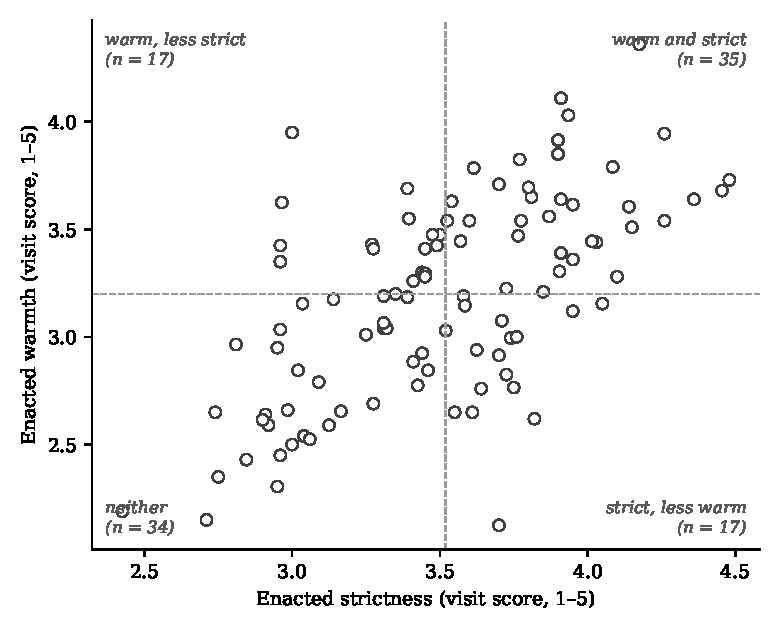
\includegraphics[width=0.8\textwidth]{fig_quadrants_ch2.pdf}
\begin{minipage}{\linewidth}\smallskip
\footnotesize\textit{Notes:} Each dot is a school. Dashed lines mark the sample medians, which divide the schools into the four labelled quadrants. All four are occupied: warm and strict; warm, less strict; strict, less warm; and neither.
\end{minipage}
\end{figure}

The second is that what heads say and what observers see are different measures. The interview and
visit scores are correlated at only $\GoldWarmthSplit$ for warmth ($p = \GoldWarmthSplitP$) and
$\GoldStrictnessSplit$ for strictness ($p \GoldStrictnessSplitP$), on the \NTierOne{} schools
with both.

Both scores are measured with error, so the highest correlation they could reach is below one. Correcting for the error in both raises warmth to $\DisSplitW$ and strictness to $\DisSplitS$. Neither reaches the value two error-free measurements of the same quantity would give, and the shortfall is much larger for warmth: heads place their school's strictness with some accuracy and its warmth with very little. The disagreement on warmth is therefore real, not a product of measurement error.

\subsection{What the public text contains}

This section shows three things. First, scores derived from public text do correlate with the enacted scores, but only when the text is an inspection report: every text measure that passes the tests comes from an inspection report, and the documents schools write about themselves carry no signal. Second, within the reports the two dimensions are read by different methods: the prediction model predicts warmth, the mark scheme scores strictness, and both work for teaching. Third, the measures the chapter goes on to use pass the three checks set out in the measurement section.

\Cref{fig:p1_validation} plots the warmth scores from the prediction model and the strictness
scores from the mark scheme against the enacted scores: the warmth model's held-out predictions
on the left, the strictness scheme's bands on the right. In both panels the two rise together:
schools the model reads as warmer are schools the observers scored as warmer, and reports the
scheme places in higher bands come from schools the observers scored as stricter. The relationship
is loose, with exceptions at every level, but it is not the work of a few outlying schools.

\begin{figure}[htbp]
  \centering
  \caption{The warmth model and the strictness scheme against the enacted scores}
  \label{fig:p1_validation}
  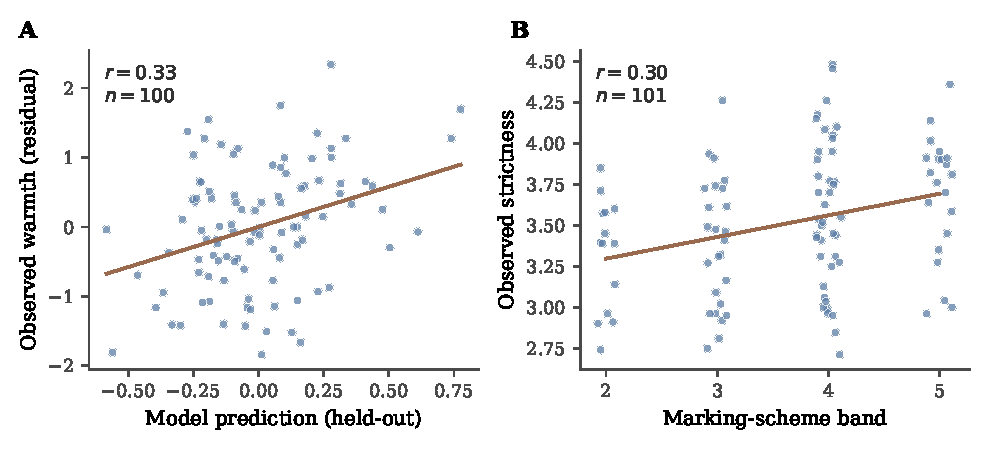
\includegraphics[width=\textwidth]{fig_ch2_validation.pdf}
\begin{minipage}{\linewidth}\smallskip
\footnotesize\textit{Notes:} Panel A shows the warmth prediction model's held-out predictions against enacted warmth, both after the demographic adjustment, that is, the part of each score that the four control variables do not explain; each school is predicted by a model that never saw it. Panel B shows the strictness mark scheme's bands against enacted strictness without that adjustment, so the correlation shown is the raw $\RubricSOfstedRaw$; the adjusted figure, $\RubricSOfstedDec$, is the one in \cref{tab:p1_grid}.
\end{minipage}
\end{figure}

\Cref{tab:p1_grid} reports fourteen text measures: seven pairings of a source with a dimension, each scored twice, once by the prediction model and once by the mark scheme. Each measure is summarised by one number: the correlation between the score it gives a school and the score the observers gave it. Each measure then faces two tests: it must beat luck, and it must stay significant once the number of tests is allowed for. Every measure that passes both tests comes from an inspection report, and none of the measures taken from the documents schools write about themselves passes either. Within the reports, warmth is read by the prediction model and strictness by the mark scheme. The rest of this section works through the tests in \cref{tab:p1_grid} and then the three checks, one at a time.

% generated by make_grid_numbers.py — do not edit
\begin{table}[htbp]
\centering
\caption{What each public text carries about enacted culture: two readings,
one criterion. Cells are correlations with the visit scores on the visited
schools ($n \approx 100$), with intake and report age partialled out of the
target. ``Agree'' is exact band agreement between the two language models
reading the same marking scheme; ``Retest'' is exact agreement on thirty
documents re-scored by the primary model.}
\label{tab:p1_grid}
\begin{tabular}{llcccc}
\toprule
Source & Dimension & Prediction model & Marking scheme & Agree & Retest \\
\midrule
Inspection report & Warmth & +0.33 & -0.07 & 68\% & 97\% \\
Inspection report & Strictness & +0.19 & +0.25 & 71\% & 100\% \\
Inspection report & Teaching & +0.28 & +0.27 & 72\% & 97\% \\
Behaviour policy & Warmth & +0.15 & +0.04 & 62\% & 83\% \\
Behaviour policy & Strictness & -0.15 & -0.03 & 72\% & 100\% \\
Website & Warmth & +0.14 & -0.13 & 31\% & 97\% \\
Website & Strictness & +0.17 & +0.13 & 39\% & 97\% \\
\bottomrule
\end{tabular}
\end{table}


The scrambled scores say how easily each of the model's results could be luck. Its three inspection-report measures all beat luck (permutation test, warmth \PermPOfstedW{}, teaching \PermPOfstedT{}, strictness \PermPOfstedS{}). Its measures from the behaviour policies and the websites all fail to.

The prediction model can be given several documents at once and the mark scheme cannot, so these pooled results are for the model alone. Each figure is again the correlation between the model's predictions and the observers' scores. Pooling the behaviour policy and the website, the two documents the school writes, gives a correlation with enacted warmth of $\PredBPWebW$; for strictness and teaching the pooled correlations are near zero. So pooling adds no signal that the separate readings missed. It can also lose one: the website on its own correlates with enacted strictness at $\PredSWeb$, and adding the policy leaves $\PredBPWebS$. Pooling all three sources never improves on the best single source; on observed teaching the correlation falls from $\PredTOfsted$ for the inspection report alone to $\PredTCombined$ for the three together.

Fourteen measures also give luck fourteen chances, so the measures in \cref{tab:p1_grid} are corrected for the number of tests as well. Four pass this test: the model's warmth and teaching, and the scheme's
strictness and teaching (the strictness scheme at $q = \QGridSOfsted$).

The prediction model predicts enacted warmth from a report's wording, correlating at $\PredWOfsted$, and enacted teaching at $\PredTOfsted$, and both figures
are essentially unchanged, or higher, when everything demographics could explain is removed.
Strictness is different: no prediction model predicts it well. The best attempt reaches
$\PredSOfsted$, it beats luck only narrowly (\PermPOfstedS{}), and its confidence interval
touches zero ($\CIPredSOfsted$). Every word-count representation tried showed the same weakness.

For strictness the mark scheme does better than the prediction model, although the gap between the two is small enough to
be chance
at this sample size ($z = \StrictDiffZ$, $p = \StrictDiffP$). The numbers alone therefore cannot
separate the two methods on strictness. The three checks set out in the measurement section
can: the retest, the change of language model, and the length check. The scheme's strictness bands pass all three.

The retest asks whether the language model gives the same answer twice. Each scheme was run
twice on the same documents. Across the seven mark schemes, the two runs give the same
band \GridRetestExact{} of the time, and the report strictness scheme gave every school
the same band on both runs.

The purpose of changing the language model is to check whether the reading is genuinely down
to the mark scheme or whether the particular model that applies it makes a difference.
If the scheme is doing the work, a different model applying the same mark scheme should find the same thing. For strictness, the second model's bands correlate with the enacted scores at $\RubricSFourO$, close to the primary model's $\RubricSOfstedRaw$, so the
scheme is what determines the band, not the model. The warmth and teaching schemes fail
the same check. Applying the same mark schemes, the second model's bands correlate with the enacted scores at essentially nothing ($\RubricWFourO$ for warmth, $\RubricTFourO$ for teaching), so what the
primary model found there came from the model rather than the scheme.

The length check asks whether the mark-scheme bands follow document length rather than the school. For the inspection-report schemes the worry is small: the strictness bands correlate with length at $\LenOfstedS$ and the warmth bands at $\LenOfstedW$, and removing the effect of length moves the strictness correlation only from $+0.25$ to $\RubricSOfstedLenP$. The website schemes' bands follow length closely, one more reason their bands are not used.

Demographic adjustment is separate from the three checks, and it is applied to the mark-scheme bands in the same way as to the prediction models' predictions; \cref{sec:p1_app_prediction} gives the specification. The adjustment changes the strictness correlation little: the scheme's correlation with enacted strictness is $\RubricSOfstedRaw$ raw and $\RubricSOfstedDec$ adjusted. The warmth scheme's bands, by contrast, correlate with enacted warmth at $\RubricWOfstedDec$ and put three-quarters of schools in one band. The model, on the same reports, predicts enacted warmth at $\PredWOfsted$,
and its advantage is itself significant (paired test, $p = \WarmDiffP$).

The two dimensions appear in the reports differently. Warmth is associated with many small differences in word choice across the whole report. A model that counts words can learn these from the visited schools, but a mark scheme cannot list them in advance. Strictness is associated with a few specific claims, for example that disruption is rare or that rules are applied consistently. A reader must be told to look for these claims. A word-count model cannot use them, because a report that says disruption is rare and one that says it is not rare use almost the same words. Teaching, kept in the
analysis as the rival explanation for the next chapter, sits in between and is read about
equally well by both methods. However, only the model's predictions pass the change-of-model check (the second model's teaching bands correlate at $\RubricTFourO$), so
the prediction model scores are used for teaching.

Behaviour policies and websites tell neither method anything about enacted culture. The prediction
models reach at most $\OwnVoiceMax$ on any pairing, too little to distinguish from zero at this
sample size, and the bands from the mark schemes correlate less still. One of those two failures needs a caution. The
two schemes that read the behaviour policies, one for warmth and one for strictness, each put
nearly every school in the same band, and a scheme that gives nearly every school the same score
cannot correlate with anything, whatever the policies contain. Its zero is therefore not evidence that the policies say nothing. The evidence comes from the prediction models. They give different schools different scores, so a signal in the policies could have shown up, and none does.

\subsection{Which parts of a report the prediction models use}

The prediction models learn which words and phrases predict the enacted scores, and nothing in the method restricts them to any topic. A model can therefore predict the enacted scores accurately for two reasons. The first is that it has picked up the words inspectors use when they describe the dimension itself, such as the way staff and pupils treat one another in the case of warmth. The second is that it has picked up the positive tone that runs through a report on a good school whatever the topic. Warm schools tend to be good schools, so a model that has learned only the general tone would still predict warmth, but it would not be reading warmth. As an informal check on the method, I annotated the content of the reports and asked whether the sentences that raise each model's predicted score most are consistent with the dimension it is meant to measure. For example, are the sentences that predict warmth about relationships between staff and pupils? For the annotation, a language model read every sentence of every report and tagged what the sentence is about: relationships, behaviour, teaching, or something else. The tagging was produced without seeing the schools' scores or anything the models learned, so it can be used to check what they learned.

The check takes the hundred sentences that raise the warmth model's predicted score most, where a sentence's contribution is the sum of the weights the model has learned for the phrases in it, and asks what they are about. \WarmTopShare{} of them are about staff--pupil relationships, against a base rate of \WarmBaseShare{} across all sentences, so the sentences that raise the warmth score are about relationships far more often than chance would give. For teaching the corresponding shares are \TeachTopShare{} against \TeachBaseShare{}, which is no enrichment at all. Inspection reports are mostly about teaching already, so the sentences that raise the teaching score cannot be about teaching much more often than the rest are. The teaching model therefore picks up the report's general tone rather than any one topic.

The topic shares, together with the demographic adjustment reported earlier, say what a model's score is made of. Part of it is language specific to the model's dimension: for warmth, the relational sentences the model seeks out. The rest is the general tone of a school doing well, which runs through a good school's whole report whatever the sentence is about. The demographic adjustment removes some of that general tone, but only the part that the four control variables (three intake measures and report age) can predict; the remainder stays in the score. A predicted warmth score therefore combines two things. Part is the relational language specific to warmth. Part is the general positive tone of a report on a good school. It is a measure of the report's whole account of the school, weighted towards warmth, not a measure of warmth alone.

\Cref{tab:p1_examples} shows the sentences each model weighs most heavily, under selection rules
stated with the table. The two listings differ. For teaching the strongest sentences name the
topic directly. For warmth they do not.

For teaching, the strongest sentences are about pedagogy: choosing core knowledge, embedding
learning in long-term memory, pupils focusing in lessons. Some of the strongest, though, are
criticisms. A sentence saying that pupils are not remembering knowledge deeply raises the score
as surely as one saying that they are. That happens for two reasons. The first is a flaw in the model. It counts words and cannot tell praise from
criticism. The second is a fact about reports. Inspectors write about long-term memory, whether in praise or criticism, only when a school teaches in that way, so the vocabulary is informative either way. The appendix discusses both in more detail.

For warmth the pattern is different, and at first sight stranger. The sentences that most lower
a school's warmth score sound kind. ``Many pupils feel confident they have a `trusted adult' they
can go to'' and ``pastoral support is in place'' are among the strongest score-lowering sentences.
The explanation for this is that an inspector writes about a warm school by describing adults and
pupils dealing with one another. When there is nothing like that to describe, the inspector
mentions support systems instead. Systems are what gets written about when the relationships
are missing.

On the positive side, no single sentence carries much weight. The model's warmth evidence is
spread across many small choices of phrase: attentive verbs, pupils' names used, care described
in passing. Even its strongest whole sentences read as the tone of an engaged community rather
than tenderness. The spread is a fact about warmth, not a weakness of the model. Warmth never
concentrates in one sentence, so there is no quotable line to point to. The case that the model
is reading warmth therefore rests on two things shown already. The first is the held-out
correlation with the warmth scores for the visited schools. The second is the topic shares:
the sentences that raise the model's predicted warmth most are
about staff--pupil relationships far more often than their share of all sentences would
predict. \Cref{sec:p1_app_examples} also lists the sentences about warmth towards staff that raise the predicted score: schools whose leaders listen to their teachers are predicted to be warmer. That
part of the signal is easy to interpret, and it is not difficult to imagine that a school
where leaders listen to staff is also one where teachers listen to the concerns of their pupils.

% generated by make_ch2_examples.py -- do not edit
\begin{table}[htbp]
\centering
\caption{Sentences from the visited schools' inspection reports that most raise or lower the models' scores. A sentence's score is the sum of its phrases' learned weights; the full listing is in \cref{sec:p1_app_examples}.}
\label{tab:p1_examples}
{\small\begin{tabular}{p{0.93\textwidth}}
\toprule
\multicolumn{1}{l}{\emph{Warmth --- raises the score}} \\
``They are taught how to show respect for different opinions and listen to the views of others.'' \\
``They hold leaders strictly to account for the quality of the school's provision and are highly effective.'' \\
``They listen to others and express their views in a well-managed environment.'' \\
``Sixth-form students are proud role models and make a highly positive contribution to the school and local community.'' \\
\addlinespace
\multicolumn{1}{l}{\emph{Warmth --- lowers the score}} \\
``However, some pupils, particularly some disadvantaged pupils, are absent too often.'' \\
``Many pupils feel confident they have a `trusted adult' they can go to.'' \\
``(Information for the school and appropriate authority)  In some subjects, the work given to some pupils does not enable them to develop their ideas and extend their answers.'' \\
``Pupils take part in a range of extra-curricular activities to develop their talents and interests, for example basketball, choir, photography, and cookery.'' \\
\addlinespace
\multicolumn{1}{l}{\emph{Teaching --- raises the score}} \\
``Those responsible for governance know the school's context and provide support and professional challenge where necessary to ensure that the school's high standards are maintained.'' \\
``Leaders are supported and challenged by dedicated and knowledgeable governors, who share their vision of high standards in a supportive school.'' \\
``In a few subjects, however, pupils are not remembering knowledge deeply in the long term.'' \\
``The school's motto is `excellence with care.' Pupils testify to how this works in practice.'' \\
\addlinespace
\multicolumn{1}{l}{\emph{Teaching --- lowers the score}} \\
``The personal, social and health education (PSHE) curriculum is designed to support pupils' wider development.'' \\
``Pupils take part in a range of extra-curricular activities to develop their talents and interests, for example basketball, choir, photography, and cookery.'' \\
``On other occasions, adults do not support pupils to complete work to a high standard.'' \\
``Judgements in this report are based on the current inspection framework and also reflect changes that have happened at any point since the last graded inspection.'' \\
\addlinespace
\bottomrule
\end{tabular}}
\end{table}


\subsection{What schools write about themselves}

A school's own documents, its behaviour policy and website, tell a reader what the head says about the school, not what the school does. The test is a rerun of the prediction models: they read the policy and website text as before, but this time they are trained to predict the head's interview answers rather than the enacted scores. This was done across the roughly 300 interviewed schools. On strictness the documents match what the head says: the models predict the head's account at $\PredEspS$ (demographics removed), which survives the correction for the number of tests. On staff morale the relation is weaker, at $\PredEspClim$: significant on its own, but not after that correction. On warmth there is no relation at all, at $\PredEspW$. What a school writes about warmth is unrelated even to what its own head says in the interview.

The bands from the website mark schemes do not correlate with any enacted or espoused score, on any dimension. That is weak evidence rather than contrary evidence: two language models applying the same website mark scheme agree on the band only \AgreeWebW{} and \AgreeWebS{} of the time, against \AgreeOfstedW{} to \AgreeOfstedT{} on inspection reports, so the scheme is barely reliable on the documents schools write about themselves.

One caveat qualifies that last result. The espoused warmth score is built from just three interview
statements, and heads bunch their answers near the top of the scale, so the score varies little
from school to school. When the target score varies little between schools, any correlation with it is lower than it would be if the scores were spread out. Finding no correlation against such a target therefore rules out a strong link between public warmth language
and the head's account, but not a modest one.

The inspection report at first seems to break this pattern. Its text correlates with the head's account of strictness at $\CrossWireRaw$, as if the inspector somehow knew what the head thinks. There is a simpler explanation. The report describes what the school does, and what the school does is itself related to what the head says. If that is the route, the report is linked to the head only through the school, and the inspector never needed to know the head's views at all. The test removes from both measures the part that enacted strictness predicts and correlates what remains. The correlation falls from $\CrossWireRaw$ to $\CrossWireNet$. So much of the link between the report and the head's account is explained by the school's actual behaviour, which both describe. The report describes the school. The head's account also describes the school. That is why the two agree, and the inspector did not need to know the head's views. So the two kinds of document line up with the two measures. What a school writes about itself matches what its head says, the espoused side. What the inspectorate writes about the school matches what the school does, the enacted side.

\subsection{A check against the parent survey}
\label{sec:p1_pv}

The last check comes from parents. Everything so far has judged the prediction model's warmth scores against the visited schools, and there are only 103 of them. Parents offer a second, independent judge at national scale: Ofsted's Parent View survey asks them, at nearly every school in England, whether their child is happy at the school and feels safe there, which is warmth as a parent experiences it. If the model's warmth scores are real, they should agree with what parents report. This section makes that comparison and reports two results: the model's warmth scores do agree with the parents, and the agreement is not explained by the inspection grade.

The measure is the parent-reported warmth score: the share of parents who say their child is happy at the school and feels safe there. There are two important limitations to this data that should be kept in mind.
The first is that parents choose whether to
respond, and the typical school's figure rests on about 120 replies, roughly one parent in eight.
The second is a timing issue. Responses are taken over several years, so at some schools the
parents' answers describe an earlier version of the school than the one the culture data describe.

The first result is the national agreement. The warmth prediction model was estimated on the visited schools alone. That leaves \PVPredWarmthN{} schools the model
has never seen. For each of these, the model reads the school's inspection report and turns it
into a predicted warmth score. Those predictions can then be set against what parents say.
Across the \PVPredWarmthN{} schools, predicted warmth and parent-reported warmth correlate at $\PVPredWarmth$; \cref{fig:p1_pv} plots the two measures against each other. That agreement would mean nothing if the model had been given the answer: two measures agree trivially when one was built from the other, as when a model
is tested on the data it was trained on. Neither is the case here. The model never saw these schools when it was estimated, and it never saw any parent data at all. The only way it can agree
 with the parents is if both are picking up something true about the school.

\begin{figure}[htbp]
  \centering
  \caption{Predicted warmth and parent-reported warmth, nationally}
  \label{fig:p1_pv}
  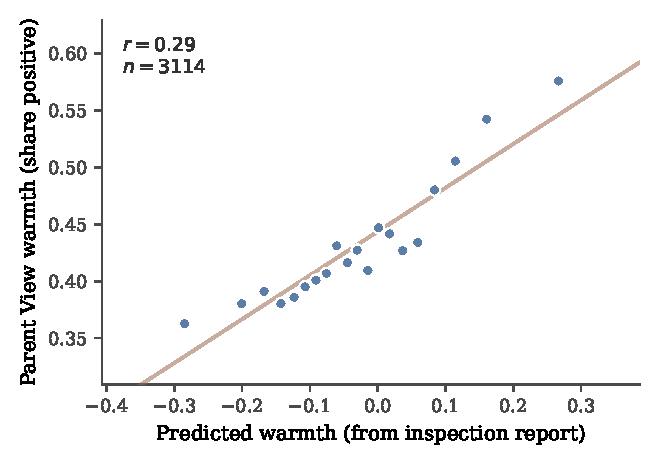
\includegraphics[width=0.55\textwidth]{fig_ch2_pv.pdf}
\begin{minipage}{\linewidth}\smallskip
\footnotesize\textit{Notes:} Correlation $r = \PVPredWarmth$ on $n = {}$\PVPredWarmthN{} schools. Each dot is a bin of schools (twenty equal-count bins); the model never saw any of these schools in training.
\end{minipage}
\end{figure}

The second result concerns the inspection grade. The model reads inspection reports, and a report reflects the grade the school received. If the model's warmth score were the grade in different words, the parents' agreement with the model would add nothing beyond the parents' agreement with the grade. The test is to compare schools that share the same grade. Within such a group the grade is the same for every school, so it cannot explain why the model scores one school warmer than another. On the visited schools, 99 of which have a grade from an inspection before the pandemic, the 2019 grade used in the next chapter, the model's correlation with enacted warmth is $+0.32$, essentially its full-sample value of $+0.33$. Comparing only schools with the same grade leaves it at $+0.29$. The teaching model gives the same result. Its correlation with enacted teaching is essentially unchanged when only schools with the same grade are compared. The model's warmth scores are not the grade in different words. \Cref{sec:p1_app_parents} adds a stricter version of this check, together with what the visited schools show and a check on one possible route: some reports quote the Parent View survey, so the model could in principle be reading the parents' answers
rather than independently agreeing with them.

The wider point is that the two measures, the parents' survey answers and the model's warmth scores, share nothing that could make them agree for any reason other than the school.
There is a final point to consider, though.
A school that is good in general tends to have both a report the model scores as warmer and happier parents, so
part of the agreement may reflect general quality rather than warmth in particular. The
agreement therefore stands as corroboration rather than proof.

\section{Conclusion}
\label{sec:p1_conclusion}

Warmth and strictness can both be measured by observation and in public text. Warmth is the harder
of the two to measure. In person it needs more lessons and more settings than
strictness does to reach the same reliability. In public text it is detected only by a model that counts words and phrases. The words associated with warmth are many and each matters a little, so they are spread across an inspection report's ordinary wording, in whether the inspector
writes about adults attending to pupils or falls back on stock assurances. A mark scheme asks the language model to find sentences that describe warmth, and no single sentence does.

Strictness is the opposite. In person it is easy to observe reliably. In text it sits in specific
claims: whether disruption is rare, whether rules are enforced consistently. Checking claims is necessary
because a report saying that disruption is rare and one saying that it is common use
almost the same words. That is why the prediction model predicts strictness weakly but the mark scheme does better.

The documents schools write about themselves match what heads say about strictness and staff morale. On warmth they carry no signal detectable at this sample size, either against the
observers or against what headteachers say when interviewed.

The parent surveys provide a useful check. At the national level their reports of happy, safe children
agree with the model, which supports the claim that inspection reports carry a real warmth signal.
In the visited schools, as the appendix shows, parents' answers are closer to the head's account than to the observers' scores.

There are four limitations that should be noted. The first is that the visit scores measure
warmth and strictness with error. Two observers watching the same school agree well but not
perfectly, so part of each score is error, and every correlation with the visit scores is lower than it would be without that error. The reported correlations therefore understate the true relations. The second is that inspection reports are written in different years under
different inspection frameworks, which adds noise. Removing dates, boilerplate and framework-specific wording reduces that noise but cannot remove it.
This kind of noise pushes correlations towards zero.

The third limitation is that each school was visited once. A visit is a
snapshot, and a school may have had an unusually calm or an unusually rough day; the scores
cannot tell an unusual day from an ordinary one.

The final limitation is that the model's warmth scores cannot be fully separated from the inspection's overall verdict. The prose
the model reads and the grade the inspection awarded come from the same visit and say
related things, so part of what the model reads may be the inspection's judgement of the
school rather than its warmth in particular. The checks in the results show that the model
reads more than the grade alone. What they cannot show is how much of the rest is warmth,
because the grade and the prose come from the same visit, so the grade already reflects some of the warmth the prose describes. Any comparison that removes the grade therefore removes part of the warmth signal as well.

With those limitations noted, the chapter provides three national measures, each validated against direct observation: prediction models for warmth and teaching, and a one-page mark scheme
for strictness. The following chapter uses these to investigate the associations between
warmth, strictness, teaching and pupil progress.

\startchapterappendix{2}
\begin{center}
  {\LARGE\bfseries Appendix to Chapter 2}\\[6pt]
  \rule{0.5\linewidth}{0.4pt}
\end{center}
\medskip
\noindent This appendix collects the supporting material for the chapter,
in the order in which the chapter uses it. It sets out how the visit and
interview items combine into scores, reproduces the two observation forms and
the interview guide as they were administered, gives the inter-rater
reliability tables, describes the samples and the coverage of the text
collections, specifies the prediction models, lists the sentences and phrases those models weigh most heavily, collects the further checks on the parent comparison, and finally reproduces the text of every mark scheme given to the language model.
\medskip

% - - - - - - - - - - - - - - - - - - - - - - - - - - - - - - -
\section{Scoring Guide and Item Definitions}
\label{app:2A:guide}

This section sets out how the individual items on the forms combine into
the nine sub-scores and the two sets of scores. The items themselves, that
is, the question wording, the response format and the anchor description
attached to each rating level, are reproduced in full in
\cref{app:2A:interview_guide} for the interview and in
\cref{app:2A:visit_protocol} for the two observation forms.

Every item is recorded on a 1--5 scale. Two observation items can also take
a zero, with a distinct meaning in each case. A zero on \emph{response of
pupils to sanctions} records that no sanction was issued during the lesson,
and a zero on \emph{effectiveness of pupil discussion} records that no
discussion was initiated. For the reasons given in the chapter, the first of these is not a genuine low score. It is replaced by $6 - \text{disruption}$, which gives a calm unsanctioned lesson a high value
and a disrupted unsanctioned lesson a low one. The second is treated as a
genuine negative, since a lesson containing no discussion did not achieve
effective discussion.

Observation item scores are averaged across lessons and across researchers
to give one value per school before the sub-scores are formed.
\Cref{tab:p1_subscore_items} lists the constituent items of each sub-score.

% Auto-generated by thesis/make_instruments.py --- do not edit by hand.
% Source: warm_strict_scorer.py

\begin{longtable}{@{}p{0.055\linewidth}p{0.235\linewidth}p{0.62\linewidth}@{}}
\caption{Composition of the gold-standard sub-scores. Item wording is given in full in \cref{app:2A:interview_guide} and \cref{app:2A:visit_protocol}.}
\label{tab:p1_subscore_items}\\
\toprule
& Sub-score & Constituent items \\
\midrule
\endfirsthead
\toprule
& Sub-score & Constituent items \\
\midrule
\endhead
\bottomrule
\endfoot
\multicolumn{3}{@{}l}{\textbf{Warmth}} \\
W1 & Teaching warmth & \textit{Lesson observation.} Frequency with which teacher uses pupils' names; Frequency of praise; Quality of interactions between teachers and pupils \\
W2 & School warmth & \textit{Outside-of-lessons observation.} Quality of relationships between pupils during transition; Quality of non-behaviour related interactions between staff and pupils at break; Quality of relationships between pupils at break \\
W3 & Headteacher warmth philosophy & \textit{Interview.} Q7 Extracurricular provision; Q11 Pupil wellbeing; S2 Reward systems applied consistently; S7 Pupils feel safe at school; S8 Pupils feel their teachers care \\
\addlinespace
\multicolumn{3}{@{}l}{\textbf{Strictness}} \\
S1 & In-lesson strictness & \textit{Lesson observation.} Level of misbehaviour tolerated before a first sanction (reversed); Frequency of low-level disruption (reversed); Response of pupils to sanctions; Extent to which pupils address the teacher respectfully \\
S2 & Out-of-lesson strictness & \textit{Outside-of-lessons observation.} Consistency of use of sanction system; Calmness of corridors; Arrival time to next lesson; Organisation of canteen/dining hall; Organisation of recreational space \\
S3 & Systems strictness & \textit{Interview.} Centralised detentions; Internal exclusion room; Behaviour points/demerits; Line-ups; Silent corridors; After-school revision; Weekend revision; Ban on mobile phones \\
S4 & Headteacher strictness philosophy & \textit{Interview.} Q5 Reward and sanction system; S1 Sanction systems applied consistently; S5 Pupil behaviour in class is generally good; S6 Pupil behaviour outside class is generally good; S9 Teachers feel respected by pupils \\
\addlinespace
\multicolumn{3}{@{}l}{\textbf{Teaching practice}} \\
T1 & Teaching practice (observed) & \textit{Lesson observation.} Frequency of questioning/checking pupil progress; Quality of verbal feedback; Effectiveness of pupil discussion; Quality of differentiation; Clarity of teacher explanation; Extent to which learning outcomes are achieved; Effectiveness of teaching methods; Clarity of lesson structure; Effectiveness of resource use \\
T2 & Teaching practice (stated) & \textit{Interview.} Q6 Characteristics of an outstanding teacher; Q8 Marking and feedback; Q12 Assessing pupil progress; S3 Teacher turnover is low; S4 Staff morale is good \\
\end{longtable}


Every other sub-score is the mean of its items, computed over the items
present so that a missing item reduces the number of contributing items
rather than the school's score.

The sub-scores combine into two sets of scores, grouped by source, with
observed behaviour and stated philosophy kept apart:
%
\begin{align}
\text{Enacted:}\quad
  W^{\text{enac}} &= \overline{(W1, W2)}, &
  S^{\text{enac}} &= \overline{(S1, S2)}, &
  T^{\text{enac}} &= T1 \label{eq:enacted} \\
\text{Espoused:}\quad
  W^{\text{esp}}  &= W3, &
  S^{\text{esp}}  &= S4, &
  \mathrm{SC} &= \overline{(\text{SC}_{1}, \text{SC}_{2})} \label{eq:espoused}
\end{align}
%
There is no espoused teaching score. The two interview statements under the
teaching heading concern staff turnover and morale, and they form the staff-climate score SC instead. The systems count S3 enters no espoused score.

Schools with an interview but no visit have the espoused set of scores alone
(every visited school was also interviewed). No imputation is attempted across the two sets: as the chapter reports, the espoused and enacted scores are too weakly correlated for either to stand in for the other.

The mapping in \cref{tab:p1_subscore_items} is generated directly from the
scoring code, so it cannot drift from what the scoring code does.

The assignment of items to dimensions is theoretical, but it can be checked
against the data. A two-factor analysis of the school-level item means
(principal components with varimax rotation, on the 98 schools with every
culture item observed) recovers most of the structure Table~2A.1 imposes:
fourteen of the nineteen culture items load most heavily on their assigned
dimension, with the in-lesson strictness items and the relational items
separating most cleanly. The remaining five load more on the other dimension. Those five are either near-ties or weakly loaded items about order in transitions. When the ten teaching items are
added they form the dominant factor, and eighteen of the nineteen culture
items then sort with their assignment. The analysis forces the two factors to be uncorrelated, while the chapter estimates the two dimensions correlate at about $0.36$. Items that belong to both are therefore harder for this method to assign, and the check is if anything conservative.

\clearpage
% - - - - - - - - - - - - - - - - - - - - - - - - - - - - - - -
\section{School Visit Protocol}
\label{app:2A:visit_protocol}

% Auto-generated by thesis/make_instruments.py --- do not edit by hand.
% Source: Novel Data/School Visit Proforma - *.docx

Two proformas were used on each visit. The lesson observation form was
completed once per lesson observed, and the outside-of-lessons form once per
school, covering transitions, break and lunch. Every item is rated 1--5 against
the anchor descriptions below, with anchors specified at 1, 3 and 5 and even
values used for intermediate judgements. Visits were made by teams of two or
three researchers, who completed the forms independently; item scores are
averaged across researchers and across lessons to give one value per school,
and \cref{sec:p1_irr_obs} reports agreement between observers.

\subsection*{Lesson observation}

\subsubsection*{Section 1 --- Strictness and Warmth}

\paragraph{Level of misbehaviour that results in a first sanction/level of misbehaviour which is tolerated}
Rated 1 (minor) to 5 (serious).

\begin{description}
\item[1] Isolated instances of misbehaviour such as whispering or fidgeting.
\item[3] Repeated disruptions, e.g., repeated talking or distraction of peers.
\item[5] Aggressive or defiant behaviour
\end{description}

\paragraph{Response of pupils to sanctions}
Rated 1 (very poor) to 5 (very good). A score of 0 is recorded separately (see below).

\begin{description}
\item[0] If no sanctions are observed
\item[1] Students ignore sanctions or react defiantly, showing no change in behaviour.
\item[3] Noticeable change in behaviour in response to sanctions, but not consistently maintained.
\item[5] Immediate and sustained positive response to sanctions e.g. apologises for actions.
\end{description}

\paragraph{Frequency of low-level disruption}
Rated 1 (very low) to 5 (very high).

\begin{description}
\item[1] Classroom is calm with disruptions rare or not occurring at all.
\item[3] Regular disruptions, sometimes affecting the flow of the lesson but generally manageable.
\item[5] Constant disruptions, creating a challenging environment for teaching and learning.
\end{description}

\paragraph{Concentration level of students}
Rated 1 (very low) to 5 (very high).

\begin{description}
\item[1] Students are consistently off-task, showing little interest or engagement with the lesson.
\item[3] Moderate levels of concentration, with students generally engaged but susceptible to distractions.
\item[5] Exceptional concentration, with students deeply engaged and consistently focused throughout the lesson.
\end{description}

\paragraph{Frequency of teacher-initiated participation}
Rated 1 (very low) to 5 (very high).

\begin{description}
\item[1] Teacher rarely encourages student participation, leading the class in a predominantly lecture-style format.
\item[3] Regular attempts by the teacher to involve students in the lesson, but some parts where teacher talks continuously.
\item[5] Teacher consistently involves students in the learning process.
\end{description}

\paragraph{Frequency of student-initiated participation}
Rated 1 (very low) to 5 (very high).

\begin{description}
\item[1] Students rarely or never take the initiative to participate, showing passivity in the learning process.
\item[3] Moderate frequency of student-initiated participation. Sometimes active but sometimes passive.
\item[5] Students consistently participate in the lesson demonstrating high levels of engagement in the learning process.
\end{description}

\paragraph{Motivation level of students}
Rated 1 (very low) to 5 (very high).

\begin{description}
\item[1] Students exhibit a lack of interest and motivation, showing little effort in classroom activities.
\item[3] A moderate level of motivation, with students showing interest at times but being disengaged at times.
\item[5] Exceptional motivation and enthusiasm, with students consistently demonstrating a strong desire to learn and participate.
\end{description}

\paragraph{Extent to which students address the teacher respectfully}
Rated 1 (not at all) to 5 (always).

\begin{description}
\item[1] Disrespectful interactions, use of inappropriate language or tone.
\item[3] Respectful interactions most of the time
\item[5] Exceptionally respectful and considerate interactions at all times.
\end{description}

\paragraph{Frequency with which teacher uses pupils' names}
Rated 1 (very low) to 5 (very high).

\begin{description}
\item[1] Rarely addresses students by name; impersonal interactions.
\item[3] Regularly uses student names, but some students are less frequently addressed.
\item[5] Consistently uses every student's name, fostering a sense of individual attention.
\end{description}

\paragraph{Frequency of praise}
Rated 1 (very low) to 5 (very high).

\begin{description}
\item[1] Teacher provides little to no praise, no positive reinforcement.
\item[3] Regular praise, but it is not always meaningful or specific.
\item[5] Regular and specific praise which highlights what students have done well.
\end{description}

\paragraph{Quality of interactions between teachers and pupils}
Rated 1 (impersonal) to 5 (warm).

\begin{description}
\item[1] Interactions are formal, distant, and lack warmth.
\item[3] Interactions are warm, but still quite formal in nature.
\item[5] Exceptionally warm and supportive interactions throughout the lesson.
\end{description}

\subsubsection*{Section 2 --- Teaching practice}

\paragraph{Frequency of questioning/checking pupil progress}
Rated 1 (very low) to 5 (very high).

\begin{description}
\item[1] Teacher rarely asks questions or checks on pupils' understanding.
\item[3] Teacher regularly asks standard questions, adequately assessing pupils' basic understanding but may not probe deeper comprehension.
\item[5] Teacher consistently integrates questioning seamlessly into lessons, skilfully using them to assess understanding and encourage higher-order thinking.
\end{description}

\paragraph{Quality of verbal feedback}
Rated 1 (very poor) to 5 (very good).

\begin{description}
\item[1] Feedback is rare, nonspecific, or irrelevant, offering no guidance or improvement for pupil learning.
\item[3] Feedback is regularly given, is clear, and somewhat constructive.
\item[5] Feedback is exceptionally well-tailored to each pupil and highly constructive.
\end{description}

\paragraph{Effectiveness of pupil discussion}
Rated 1 (not effective) to 5 (very effective). A score of 0 is recorded separately (see below).

\begin{description}
\item[0] No teacher-initiated pupil discussion is observed.
\item[1] Pupil discussions are rarely initiated or if they are, then they are poorly managed, resulting in minimal pupil engagement.
\item[3] Regularly encourages discussions which have a moderate impact on learning but may not fully engage all pupils.
\item[5] Regularly encourages discussions and structures them effectively to ensure that pupils engage with them and benefit from them.
\end{description}

\paragraph{Quality of differentiation (adaptation to students' needs)}
Rated 1 (very poor) to 5 (very good).

\begin{description}
\item[1] Teaching lacks adaptation to different learning needs, often leading to disengagement or unmet learning objectives for various students.
\item[3] Regularly employs differentiation strategies that address the needs of most students but not all.
\item[5] Exceptional in adapting teaching to meet all students' needs. Challenges high ability pupils and/or supports low ability pupils appropriately.
\end{description}

\paragraph{Clarity of teacher explanation}
Rated 1 (very poor) to 5 (very good).

\begin{description}
\item[1] Explanations are often unclear, leading to widespread confusion or misconceptions among students.
\item[3] Usually provides explanations that are clear and aid in student understanding, though some concepts may not be understood by all students.
\item[5] Provides exceptionally clear and comprehensive explanations, making complex concepts accessible to all or almost all students.
\end{description}

\paragraph{Extent to which learning outcomes are achieved}
Rated 1 (not at all) to 5 (completely).

\begin{description}
\item[1] Learning outcomes are rarely met, with most students failing to achieve the set objectives. Unclear what learning objectives are.
\item[3] A majority of learning outcomes are met, though some objectives may not be fully achieved by all students.
\item[5] All learning outcomes are fully met, with evidence of deep understanding and application of knowledge by all or almost all students.
\end{description}

\paragraph{Effectiveness of teaching methods}
Rated 1 (not effective at all) to 5 (very effective).

\begin{description}
\item[1] Teaching method(s) are not appropriate to the content and tasks.
\item[3] Teaching method(s) are mostly appropriate to the content and tasks.
\item[5] Chosen teaching method(s) are very well matched to the content and every task is clearly well thought out.
\end{description}

\paragraph{Clarity of lesson structure}
Rated 1 (unclear) to 5 (very clear).

\begin{description}
\item[1] Lessons lack a clear structure, resulting in disorganized content delivery. Structure is not communicated to students.
\item[3] Generally clear lesson structure with a logical flow, though minor issues in transition or clarity may occasionally arise. Structure is communicated quite well to students.
\item[5] Lessons are exceptionally well-structured, with seamless transitions, and a well-thought-out progression. Structure is regularly communicated to students.
\end{description}

\paragraph{Effectiveness of resource use}
Rated 1 (low) to 5 (high).

\begin{description}
\item[1] The resources do not allow most students to achieve the learning objectives and/or engage with the topic.
\item[3] The resources allow most students to achieve the learning objectives and/or engage with the topic.
\item[5] The resources allow all or almost all of the students to achieve the learning objectives and/or engage with the topic.
\end{description}


\subsection*{Outside-of-lessons observation}

\subsubsection*{Section 1 --- Comparison across lessons}

\paragraph{Consistency of use of sanction system}
Rated 1 (not consistent at all) to 5 (completely consistent).

\begin{description}
\item[1] Teachers are using different sanction systems in every classroom.
\item[3] Teachers are generally taking the same approach to misbehaviour, but there is no shared language.
\item[5] All teachers use the sanction system in exactly the same way and there is a clear shared language.
\end{description}

\paragraph{Consistency of use of reward system}
Rated 1 (not consistent at all) to 5 (completely consistent).

\begin{description}
\item[1] Teachers are using different reward systems in every classroom.
\item[3] Teachers are generally taking the same approach to positive behaviours, but there is no shared language.
\item[5] All teachers use the reward system in exactly the same way and there is a clear shared language.
\end{description}

\paragraph{Consistency of verbal feedback}
Rated 1 (not consistent at all) to 5 (completely consistent).

Should be calculated as the average of the scores from individual lessons.

\paragraph{Quality of differentiation (adaptation to students' needs) across lessons}
Rated 1 (very poor) to 5 (very good).

Should be calculated as the average of the scores from individual lessons.

\subsubsection*{Section 2 --- Transitions}

\paragraph{Calmness of corridors}
Rated 1 (chaotic) to 5 (calm).

\begin{description}
\item[1] The corridors feel unsafe. There is a lot of boisterous behaviour and students do not seem concerned with getting to their next lesson.
\item[3] Most students move between lessons in a calm fashion. There is an occasional loud voice and a small amount of boisterous behaviour. Most students move purposefully to their next lesson.
\item[5] All students move between lessons in a calm fashion with no loud voices or boisterous behaviour at all. All students move with purpose to their next lesson.
\end{description}

\paragraph{Arrival time to next lesson}
Rated 1 (lots of lateness) to 5 (all on time).

\begin{description}
\item[1] The majority of students arrive late to lessons.
\item[3] Most students arrive on time with a few late arrivals.
\item[5] All or almost all students arrive on time.
\end{description}

\paragraph{Quality of relationships between students during transition}
Rated 1 (very poor) to 5 (very good).

\begin{description}
\item[1] Lots of students speak to each other disrespectfully. There is clear evidence of bullying and/or intimidation.
\item[3] Most students are polite in their interactions with each other. There is evidence that a small amount of bullying/intimidation is taking place.
\item[5] All or almost all students are polite in their interactions with each other. There is no evidence of bullying or intimidation of any kind.
\end{description}

\paragraph{Presentation of wall/corridor displays}
Rated 1 (poor condition) to 5 (excellent condition).

\begin{description}
\item[1] There are no displays, or if there are, then they are old and tattered.
\item[3] Most displays are in good condition, but some are a bit tattered and look old.
\item[5] All displays are in pristine condition with no damage. They all look as if they are new.
\end{description}

\paragraph{Extent to which wall/corridor displays which are not student work align with school values}
Rated 1 (random) to 5 (complete alignment).

\begin{description}
\item[1] There are no displays which convey messages about the school values.
\item[3] There are some displays which convey messages about the school values.
\item[5] All or almost all displays convey messages about the school values.
\end{description}

\subsubsection*{Section 3 --- Break and lunch}

\paragraph{Quality of non-behaviour related interactions between staff and students}
Rated 1 (very poor) to 5 (very good).

\begin{description}
\item[1] In general, staff do not engage with students.
\item[3] Most staff actively engage with students and interactions are mostly warm and personal.
\item[5] All or almost all staff actively engage with students and interactions are warm and personal.
\end{description}

\paragraph{Quality of relationships between students}
Rated 1 (very poor) to 5 (very good).

\begin{description}
\item[1] Lots of students speak to each other disrespectfully. There is clear evidence of bullying and/or intimidation.
\item[3] Most students are polite in their interactions with each other. There is evidence that a small amount of bullying/intimidation is taking place.
\item[5] All or almost all students are polite in their interactions with each other. There is no evidence of bullying or intimidation of any kind.
\end{description}

\paragraph{Organisation of canteen/dining hall}
Rated 1 (chaotic) to 5 (calm).

\begin{description}
\item[1] Students get their food in a haphazard fashion. They leave food behind on tables and on the floor. They do not take care of their environment.
\item[3] There is some organisation to the way that students get their food. There is a little bit of mess left behind.
\item[5] Students get their food in an organised fashion. They leave the table and floor where they eat clean and tidy.
\end{description}

\paragraph{Organisation of recreational space}
Rated 1 (chaotic) to 5 (calm).

\begin{description}
\item[1] Activities are interfering with each other and there is no supervision from staff. There is a general sense of disorganisation. There is lots of rule breaking.
\item[3] There are clear areas for different activities, and some are supervised by staff. There is some rule breaking.
\item[5] There are clear areas for different activities, and these are all supervised by members of staff. All or almost all students abide by the rules.
\end{description}


\clearpage
% - - - - - - - - - - - - - - - - - - - - - - - - - - - - - - -
\section{Interview Guide}
\label{app:2A:interview_guide}

% Auto-generated by thesis/make_instruments.py --- do not edit by hand.
% Source: Novel Data/Headteacher Interview.docx

The schedule below is the instrument as administered. Each open-ended
question was scored 1--5 against the anchor descriptions shown. Each
question was asked by one researcher and scored by both; \cref{tab:irr_interview}
reports agreement between them, and the analysis uses the final recorded score
for each question. A checklist of key words and phrases was also completed for
each question; it enters no score reported in the chapter and is omitted here.
Item-to-sub-score mapping is given in \cref{app:2A:guide}.

\subsubsection*{Open-ended questions}

\paragraph{Q1. How long have you been in post?}
Recorded verbatim; not scored on the 1--5 scale.

\paragraph{Q2. How would you describe your school's culture?}
Rated 1 (weak answer) to 5 (strong answer).

\begin{description}
\item[1] A vague or generic description is provided, lacking specific details or examples.
\item[3] A detailed description of the school's culture, including some specific examples, but no explanation of the rationale for this culture.
\item[5] A detailed description of the school's culture with specific examples that also includes a clear explanation of the rationale for this culture.
\end{description}

\paragraph{Q3. How do you communicate this culture to your staff?}
Rated 1 (weak answer) to 5 (strong answer).

\begin{description}
\item[1] The strategies used to communicate the culture to the staff are not clearly explained.
\item[3] The strategies used to communicate the culture to the staff are clearly explained, but there is a lack of detail.
\item[5] There is a detailed and clear explanation of the strategies used to communicate the culture to the staff.
\end{description}

\paragraph{Q4. What do you think is the most important characteristic of an effective school? Why?}
Rated 1 (weak answer) to 5 (strong answer).

\begin{description}
\item[1] Various characteristics are mentioned but there is no clear explanation of why these characteristics lead to a school being effective.
\item[3] One or multiple characteristics are mentioned and there is a clear explanation of why these characteristics lead to a school being effective.
\item[5] One or multiple characteristics are mentioned and there is a clear explanation of why these characteristics lead to a school being effective. There is also a discussion of how the school culture links to these characteristics.
\end{description}

\paragraph{Q5. How does your reward and sanction system work? If a pupil misbehaves what should happen? If a pupil makes a positive contribution what should happen?}
Rated 1 (weak answer) to 5 (strong answer).

\begin{description}
\item[1] The explanation of the reward and sanction system is unclear, lacking specific details or a coherent structure.
\item[3] The response outlines the reward and sanction system to a decent extent, but there may be gaps in the explanation, and details might be limited.
\item[5] A clear and detailed explanation is provided on how the reward and sanction system operates; the response demonstrates a deep understanding of the procedures for addressing both misbehaviour and positive contributions.
\end{description}

\paragraph{Q6. What do you think are the key characteristics of an outstanding classroom teacher?}
Rated 1 (weak answer) to 5 (strong answer).

\begin{description}
\item[1] Various characteristics are mentioned but there is no clear explanation of why these characteristics make a teacher outstanding.
\item[3] Various characteristics are mentioned and there is a clear explanation of why these characteristics make a teacher is outstanding.
\item[5] Various characteristics are mentioned and there is a clear explanation of why these characteristics make a teacher is outstanding. There is also a discussion of how these characteristics link to the school's culture.
\end{description}

\paragraph{Q7. How important do you think extracurricular provision is? What kind of extracurricular provision have you put in place?}
Rated 1 (weak answer) to 5 (strong answer).

\begin{description}
\item[1] The importance of extracurricular provision is not clearly articulated, and the response lacks specific details about the types of activities available.
\item[3] The response acknowledges the importance of extracurricular provision, but the explanation may be somewhat basic or lacking in depth; details about the types of activities implemented could be more specific.
\item[5] The response shows a clear understanding of the importance of extracurricular provision and provides specific details about the types of activities in place.
\end{description}

\paragraph{Q8. What is your view on the importance of marking and feedback? Is there a school-wide policy on frequency and type?}
Rated 1 (weak answer) to 5 (strong answer).

\begin{description}
\item[1] The explanation of the importance of marking and feedback is unclear. If there is a school-wide policy, then it is also not explained clearly.
\item[3] The explanation of the importance of marking and feedback is clear. If there is a school-wide policy, then it is also explained clearly but without specific details.
\item[5] The answer lays out a clear and comprehensive view on the importance of marking and feedback. It provides specific details about a school-wide policy, including the frequency and type of marking and feedback.
\end{description}

\paragraph{Q9. What is the structure of your staff team?}
Rated 1 (weak answer) to 5 (strong answer).

\begin{description}
\item[1] The explanation is unclear and difficult to follow.
\item[3] There is a clear explanation of the staff structure from Senior Team through to Middle Leaders.
\item[5] The answer clearly lays out the staff structure from Senior Team down to classroom teachers and support staff with some explanation of the rationale for the structure.
\end{description}

\paragraph{Q10. How do you hold staff to account?}
Rated 1 (weak answer) to 5 (strong answer).

\begin{description}
\item[1] A brief answer which mentions the use of performance management structures but does not go into detail.
\item[3] A clear explanation of the performance management process with discussion of informal and formal steps.
\item[5] A clear explanation of the performance management process with discussion of informal and formal steps, as well as an explanation of an underlying philosophy.
\end{description}

\paragraph{Q11. How do you manage the wellbeing of your pupils?}
Rated 1 (weak answer) to 5 (strong answer).

\begin{description}
\item[1] An imprecise answer which emphasises the importance of managing pupil wellbeing but does not lay out any clear strategies for doing so.
\item[3] An answer which lays out strategies for managing pupil wellbeing, but some strategies are not very precise.
\item[5] An answer which lays out clear strategies for managing pupil wellbeing alongside an explanation of why this is important.
\end{description}

\paragraph{Q12. How do you assess pupil progress?}
Rated 1 (weak answer) to 5 (strong answer).

\begin{description}
\item[1] An answer which mentions no specific strategies for monitoring the progress that pupils are making.
\item[3] An answer which outlines strategies for assessing pupil progress in a summative manner only.
\item[5] An answer which outlines a range of strategies for assessing pupil progress formatively and summatively.
\end{description}

\subsubsection*{Yes-or-no questions}

Does your school make use of the following systems:

\begin{itemize}
\item Centralised detentions
\item An internal exclusion room
\item Reward assemblies/prize-giving ceremonies
\item Behaviour points/demerits
\item Reward points/merits
\item Line-ups
\item Silent corridors
\item After-school revision
\item Weekend revision
\item Ban on mobile phones in school
\end{itemize}

Would you like to say anything about your school's use of any of these systems?

\subsubsection*{Statement ranking}

For each of the following statements circle the appropriate number:

Each statement is rated 1 (strongly disagree) to 5 (strongly agree).

\begin{itemize}
\item The sanction systems are applied consistently by all staff
\item The reward systems are applied consistently by all staff
\item Teacher turnover is low
\item Staff morale is good
\item Pupil behaviour in class is generally good
\item Pupil behaviour outside of class is generally good
\item Pupils feel safe at school
\item Pupils feel like their teachers care
\item Teachers feel respected by all students
\item In general, parents are engaged with their child's education
\end{itemize}

Would you like to say anything about any of your responses to these questions?

Would you be willing to allow a few members of our team to come and observe the normal functioning of your school for a day?

\subsubsection*{To be completed after the interview}

\paragraph{Rate the confidence with which the headteacher responded to the questions}
Rated 1 (not confident at all) to 5 (confident).

\begin{description}
\item[1] There was a lot of hesitation throughout the interview and a lack of clarity in almost all the responses.
\item[3] The answers were generally clear and delivered without hesitation.
\item[5] Every answer was clear and delivered without hesitation. There were no wasted words.
\end{description}

\paragraph{Willingness to reveal information}
Rated 1 (very reluctant) to 5 (totally willing).

\begin{description}
\item[1] There was a reluctance to go into specific details throughout the interview.
\item[3] The headteacher went into specific detail with most answers, but not all.
\item[5] The headteacher was happy to go into very specific detail in every answer.
\end{description}

\paragraph{Interviewee patience}
Rated 1 (little patience) to 5 (lots of patience).

\begin{description}
\item[1] The headteacher rushed through all their answers.
\item[3] The headteacher gave detailed responses to most questions but did not add any detail to the yes/no or statement questions.
\item[5] The headteacher was happy to give detailed responses to all questions and wanted to add detail to their answers to the yes/no and statement questions.
\end{description}


\clearpage
% - - - - - - - - - - - - - - - - - - - - - - - - - - - - - - -
\section{Inter-rater Reliability Tables}
\label{app:2A:irr}

\begin{table}[htbp]
\centering
\caption{Inter-rater reliability for headteacher interview items Q2--Q12.
For each item, a questioner and an observer scored independently on a 1--5 scale.
$r$: Pearson correlation; MAD: mean absolute difference; Exact: proportion of pairs
with identical scores; W1: proportion agreeing within one scale point;
$\kappa_w$: weighted Cohen's $\kappa$ (linear weights).}
\label{tab:irr_interview}
\small
\begin{tabular}{p{5.5cm}rrrrrr}
\toprule
Item & $N$ & $r$ & MAD & Exact\% & W1\% & $\kappa_w$ \\
\midrule
Q2\enspace\textit{{What words describe your school's culture?}} & 292 & 0.709 & 0.56 & 40 & 90 & 0.537 \\
Q3\enspace\textit{{How do you communicate culture to staff?}} & 293 & 0.698 & 0.56 & 33 & 94 & 0.499 \\
Q4\enspace\textit{{What makes an outstanding teacher here?}} & 293 & 0.712 & 0.51 & 41 & 93 & 0.533 \\
Q5\enspace\textit{{How do you reward and sanction pupils?}} & 291 & 0.726 & 0.43 & 44 & 97 & 0.512 \\
Q6\enspace\textit{{What does excellent teaching look like?}} & 293 & 0.613 & 0.52 & 40 & 93 & 0.424 \\
Q7\enspace\textit{{What is your co-curricular offer?}} & 294 & 0.617 & 0.50 & 41 & 95 & 0.448 \\
Q8\enspace\textit{{How do you approach marking and feedback?}} & 294 & 0.691 & 0.48 & 42 & 94 & 0.552 \\
Q9\enspace\textit{{Describe your senior leadership team}} & 294 & 0.623 & 0.45 & 48 & 94 & 0.491 \\
Q10\enspace\textit{{How do you hold staff to account?}} & 291 & 0.707 & 0.52 & 37 & 92 & 0.547 \\
Q11\enspace\textit{{What are biggest challenges facing pupils?}} & 292 & 0.681 & 0.45 & 45 & 93 & 0.550 \\
Q12\enspace\textit{{How do you know how pupils are progressing?}} & 293 & 0.740 & 0.40 & 53 & 95 & 0.606 \\
\bottomrule
\end{tabular}
\end{table}

\begin{table}[htbp]
\centering
\small
\begin{tabular}{lrrrrrr}
\toprule
Item & $N$ & $r$ & MAD & Exact\% & W1\% & $\kappa_w$ \\
\midrule
Misbehaviour & 439 & 0.702 & 0.45 & 51 & 93 & 0.566 \\
Response & 277 & 0.669 & 0.59 & 43 & 88 & 0.545 \\
Disruption & 466 & 0.788 & 0.42 & 53 & 93 & 0.638 \\
Concentration & 467 & 0.647 & 0.51 & 39 & 94 & 0.474 \\
Teacher & 465 & 0.636 & 0.58 & 41 & 89 & 0.450 \\
Student & 457 & 0.637 & 0.63 & 37 & 88 & 0.456 \\
Motivation & 467 & 0.610 & 0.53 & 40 & 93 & 0.454 \\
Respectfully & 467 & 0.654 & 0.53 & 44 & 94 & 0.473 \\
Names & 463 & 0.698 & 0.62 & 43 & 88 & 0.524 \\
Praise & 456 & 0.688 & 0.59 & 39 & 90 & 0.525 \\
Interactions & 463 & 0.616 & 0.62 & 35 & 88 & 0.420 \\
Questioning & 468 & 0.585 & 0.61 & 38 & 89 & 0.440 \\
Verbal & 454 & 0.562 & 0.68 & 37 & 85 & 0.417 \\
Discussion & 217 & 0.722 & 0.59 & 41 & 91 & 0.542 \\
Differentiation & 437 & 0.637 & 0.65 & 38 & 84 & 0.476 \\
Explanation & 454 & 0.578 & 0.51 & 44 & 93 & 0.439 \\
Outcomes & 432 & 0.620 & 0.52 & 44 & 91 & 0.464 \\
Methods & 467 & 0.552 & 0.54 & 41 & 92 & 0.424 \\
Structure & 461 & 0.560 & 0.58 & 40 & 90 & 0.398 \\
Resource & 463 & 0.528 & 0.54 & 43 & 91 & 0.378 \\
\bottomrule
\end{tabular}
\caption{Inter-rater reliability: classroom observation items}
\label{tab:irr_classroom}
\begin{minipage}{\linewidth}
\smallskip
\footnotesize\textit{Notes:} Each row pools all pairwise comparisons across lessons observed by two or three researchers simultaneously. $r$: Pearson correlation; MAD: mean absolute difference; Exact: exact agreement; W1: within-one-point agreement; $\kappa_w$: weighted Cohen's $\kappa$ (linear weights, categories 1--5).
\end{minipage}
\end{table}


\begin{table}[htbp]
\centering
\caption{Inter-rater reliability for outside-of-lesson observation items.
Each row pools all pairwise comparisons across outside-of-lesson observation
sessions attended by two or three researchers. $r$, MAD, Exact, W1, $\kappa_w$
as defined in \cref{tab:irr_classroom}.}
\label{tab:irr_outside}
\small
\begin{tabular}{lrrrrrr}
\toprule
Item & $N$ & $r$ & MAD & Exact\% & W1\% & $\kappa_w$ \\
\midrule
Sanction & 87 & 0.714 & 0.48 & 52 & 91 & 0.610 \\
Reward & 83 & 0.805 & 0.40 & 63 & 90 & 0.706 \\
Verbal & 76 & 0.485 & 0.45 & 32 & 91 & 0.380 \\
Differentiation & 70 & 0.552 & 0.48 & 27 & 93 & 0.345 \\
Corridors & 93 & 0.657 & 0.49 & 39 & 96 & 0.515 \\
Arrival & 91 & 0.474 & 0.58 & 42 & 91 & 0.303 \\
Students & 93 & 0.705 & 0.42 & 47 & 100 & 0.491 \\
Displays & 91 & 0.548 & 0.51 & 54 & 88 & 0.522 \\
Alignment & 84 & 0.578 & 0.62 & 44 & 85 & 0.411 \\
Interactions & 86 & 0.684 & 0.58 & 36 & 92 & 0.511 \\
Relationships & 89 & 0.724 & 0.38 & 54 & 96 & 0.599 \\
Canteen & 91 & 0.727 & 0.38 & 51 & 99 & 0.515 \\
Recreational & 91 & 0.532 & 0.49 & 45 & 92 & 0.446 \\
\bottomrule
\end{tabular}
\end{table}

\clearpage
% - - - - - - - - - - - - - - - - - - - - - - - - - - - - - - -
\section{Sample Characteristics}
\label{app:2A:sample}

\subsection{Sample representativeness}
\label{sec:p1_representativeness}

\Cref{tab:2A:representativeness} and \cref{fig:2A:representativeness_region} compare the
interviewed and visited schools (300 and 102 of them matched to the school panel; 303 and
103 in all) to the national population of 3,312 open secondary and all-through schools in
England, across a range of structural characteristics drawn from the school panel spine and
the Get Information About Schools register, together with the inspection grade as at August
2024 and the pre-pandemic Progress~8 of 2018--19.

The interviewed and visited samples are broadly representative of the national population
on most structural dimensions. School type (academy, maintained, free school), phase of
education, gender composition, admissions policy, and urban--rural classification are all
closely matched to national proportions, with no statistically significant differences.
Mean school size and free school meals percentage are also similar to national averages:
interviewed schools average 1,109 pupils (national mean: 1,079) and a free school meals
share of 27.9\% (national mean: 29.9\%).

The main exception is regional distribution
(\cref{fig:2A:representativeness_region}). Both samples over-represent London and, for
interviews, the South East: taken together, London and the South East account for
44.7\% of interviewed schools versus 30.3\% nationally. The visited sample is
particularly concentrated geographically---London accounts for 45.1\% of visits compared
to 15.0\% of schools nationally---reflecting the logistical constraints of conducting
full-day school visits. Northern England is correspondingly under-represented: the North
West (13.9\% nationally, 8.7\% of interviewed, 2.9\% of visited), the West Midlands
(11.9\%, 7.7\%, 1.0\%), and Yorkshire and the Humber (9.6\%, 5.3\%, 0.0\%) all feature
substantially less in the sample than in the population. Visited schools are also more
likely to have a sixth form (nan\% versus nan\% nationally), consistent with the London
concentration given that London schools disproportionately offer post-16 provision.

Both samples also lean toward stronger schools: 25 per cent of visited schools held an
Outstanding grade as at August 2024 against 15 per cent nationally, and their mean
2018--19 Progress~8 was $+$0.17 against $+$0.04 nationally; the interviewed sample shows the
same lean more weakly (19 per cent and $+$0.08).

These patterns should be borne in mind when interpreting findings, particularly for the
visit-based tier. Warmth and strictness estimates for the primary tier
(\Cref{sec:p1_data}) may not be fully generalisable to schools in the North of England,
and cross-tier comparisons should account for the possibility that regional compositional
differences contribute to attenuation.


\begin{table}[htbp]
\centering
\small
\caption{Comparison of interviewed and visited schools to the national population of open secondary schools in England.}
\label{tab:2A:representativeness}
\begin{tabular}{ll ccc cc}
\toprule
 & & \multicolumn{3}{c}{\textit{Percentage of schools} (\%)} & \multicolumn{2}{c}{\textit{p}-value} \\
\cmidrule(lr){3-5} \cmidrule(lr){6-7}
\textit{Variable} & \textit{Category} & National & Interviewed & Visited & Int. & Vis. \\
 & & $(n=3{,}312)$ & $(n=300)$ & $(n=103)$ & & \\
\midrule
  \textit{School type} & Academy & 74.7 & 72.3 & 74.3 & \textit{ns} & \textit{ns} \\
   & Free school & 9.2 & 10.0 & 11.9 &  &  \\
   & Maintained & 15.8 & 17.7 & 13.9 &  &  \\
\addlinespace[3pt]
  \textit{Phase} & Secondary & 95.1 & 94.3 & 93.1 & \textit{ns} & \textit{ns} \\
   & All-through & 4.9 & 5.7 & 6.9 &  &  \\
\addlinespace[3pt]
  \textit{Gender} & Mixed & 89.2 & 87.7 & 85.1 & \textit{ns} & \textit{ns} \\
   & Girls & 6.1 & 7.0 & 5.9 &  &  \\
   & Boys & 4.3 & 5.3 & 8.9 &  &  \\
\addlinespace[3pt]
  \textit{Admissions policy} & Non-selective & 85.4 & 87.0 & 88.1 & \textit{ns} & \textit{ns} \\
   & Selective & 4.9 & 5.3 & 5.0 &  &  \\
\addlinespace[3pt]
  \textit{Urban/rural} & Urban & 87.4 & 88.3 & 90.1 & \textit{ns} & \textit{ns} \\
   & Rural & 12.5 & 11.7 & 9.9 &  &  \\
\addlinespace[3pt]
  \textit{Has sixth form} & Yes & 62.7 & 68.0 & 75.2 & \textit{ns} & p$<$.01 \\
   & No & 37.3 & 32.0 & 24.8 &  &  \\
\addlinespace[3pt]
  \textit{Ofsted grade (Aug 2024)} & Outstanding & 14.7 & 18.3 & 25.2 & p$<$.05 & p$<$.05 \\
   & Good & 69.2 & 70.3 & 63.1 &  &  \\
   & Requires improvement & 12.9 & 8.0 & 8.7 &  &  \\
   & Inadequate & 3.2 & 3.3 & 2.9 &  &  \\
\addlinespace[4pt]
\multicolumn{7}{l}{\textit{Continuous variables}} \\
\addlinespace[2pt]
  \textit{Number of pupils} & Mean (\textit{SD}) & 1{,}079 (396) & 1{,}109 (384) & 1{,}134 (380) & \textit{ns} & \textit{ns} \\
  \textit{FSM percentage} & Mean (\textit{SD}) & 29.9 (14.7) & 28.0 (14.7) & 29.1 (15.7) & p$<$.05 & \textit{ns} \\
  \textit{Prior P8 (2018--19)} & Mean & $+$0.04 & $+$0.08 & $+$0.17 & \textit{ns} & p$<$.01 \\
\bottomrule
\end{tabular}
\begin{minipage}{\linewidth}
\smallskip
\footnotesize\textit{Notes:} National population is all open secondary and all-through schools in England.
$p$-values are approximate: $\chi^2$ goodness-of-fit test (observed vs national proportions) for categorical
variables; one-sample $z$-test for continuous variables. Rows with $<$0.5\% share in all columns omitted.
The Ofsted-grade and prior-P8 rows are computed on the full tiers (visited $n=103$, all
graded; interviewed $n=303$, of which 300 graded; national $n=3{,}332$, of which 3,297
graded); grade tests are $\chi^2$ against the non-tier remainder (visited $p=0.019$,
interviewed $p=0.029$), and the prior-P8 rows use schools with a published 2018--19
score (national $n=2{,}731$, interviewed $n=259$, visited $n=95$; two-sample $t$-tests,
visited $p=0.003$, interviewed $p=0.087$).
Regional distribution is shown separately in \cref{fig:2A:representativeness_region}.
\end{minipage}
\end{table}

\begin{figure}[htbp]
  \centering
  \caption{Regional distribution of interviewed and visited schools}
  \label{fig:2A:representativeness_region}
  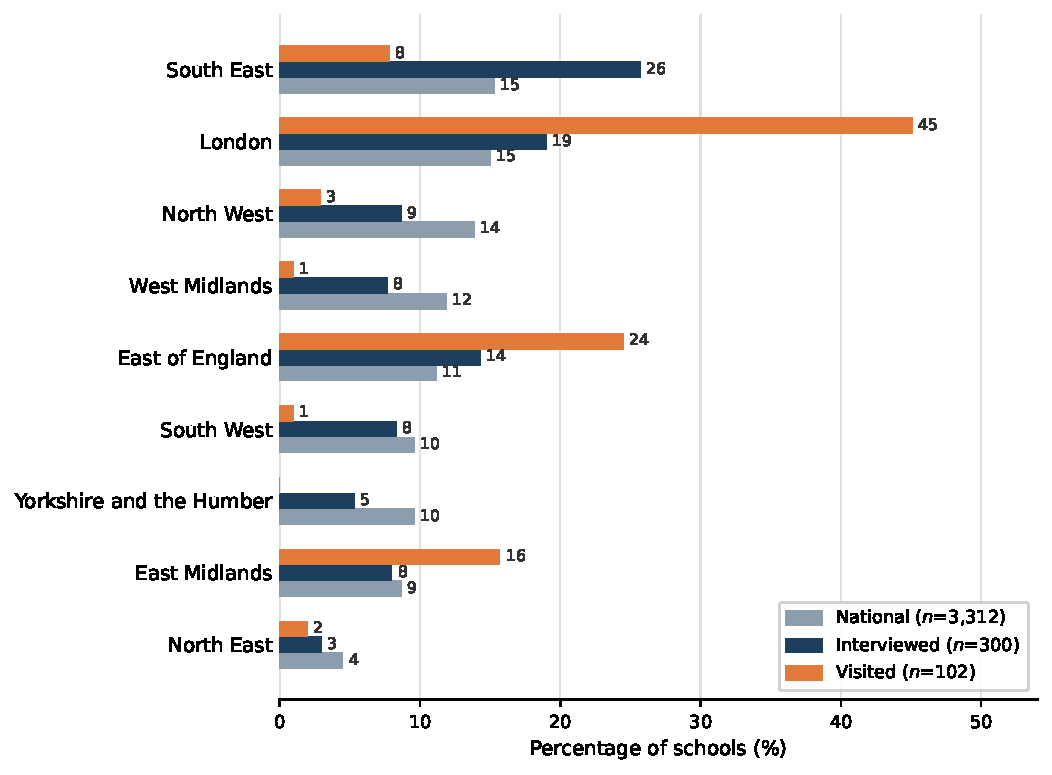
\includegraphics[width=\textwidth]{fig_D_regional_representativeness.pdf}
\begin{minipage}{\linewidth}\smallskip
\footnotesize\textit{Notes:} The comparison is with the national population of open secondary and all-through schools in England. Bars show the percentage of schools in each region for the national population ($n = 3{,}312$), interviewed schools ($n = 300$), and visited schools ($n = 102$), the schools matched to the school panel (the 2023/24 regional characteristics panel holds 3{,}312 of the 3{,}332 analysis-panel schools; the remainder lack a region record at that date). Regions are ordered by national share.
\end{minipage}
\end{figure}

\paragraph{Coverage of the text collections.} The three collections of
text were each gathered from the register of open state secondary schools at
a different date, which is why their raw counts differ. Inspection reports
were scored for 3,324 schools, behaviour policies were obtained for 3,363,
and websites were crawled for 3,370. Set against the analysis panel of 3,332 schools, the coverage counts and shares are those reported with the data: 3,272 reports, 3,294 policies and 3,311 crawls, of which 3,284 contain scorable prose. The few schools in each collection that
are outside the panel are schools that closed, merged or changed identifier
between the crawl and the construction of the panel.

\clearpage
% - - - - - - - - - - - - - - - - - - - - - - - - - - - - - - -
\section{Prediction Model Specification}
\label{sec:p1_app_prediction}

The text representation is TF-IDF over words and two-word phrases
(English stop words removed; terms kept if they appear in at least five
documents and at most ninety per cent of them; sublinear term frequency;
each document's vector normalised to unit length). The model is a ridge
regression with an unpenalised intercept, estimated exactly in kernel
form. Every reported correlation is leave-one-out: the model is re-estimated with each school excluded, and the penalty is re-chosen within every fold
by closed-form inner leave-one-out, so the held-out school takes no part in estimating the model or choosing its penalty. Predictions are clipped to the range of the
training scores. Significance comes from a permutation test: the identical
pipeline is run on two hundred permutations of the outcome, and the
reported $p$ is the share of permutations matching or beating the real
correlation.

Before modelling, documents are cleaned of identifying and clerical
material: establishment, trust and local-authority names (from the
national register), month names and years, postcodes, tokens containing
digits, inspection-report page furniture, letter salutations, and
framework boilerplate. The demographic adjustment regresses each outcome on the school's free-school-meals share, share of pupils with English as an additional language, prior attainment and report age, and takes the residual as the target. The mark-scheme bands are not changed. The adjustment is applied to the outcome only. The adjusted figure for a mark scheme is the correlation between the band as awarded and this residual.

Alternative representations were evaluated in the identical harness and none improved on the specification above. In brief, adding three- and four-word phrases moved each correlation by less than its sampling variation. Topic-model features predicted every dimension worse than word and phrase counts did. Models estimated on passage embeddings from two pretrained encoders correlate with enacted warmth and teaching at essentially zero. They do reproduce the espoused-strictness result. So the warmth and teaching signals lie in the particular words used, not in meaning that survives paraphrase. One result disagrees between the two encoders. The larger encoder predicts enacted strictness at $+0.33$ with mean pooling. The smaller encoder's correlation is near zero, and so is that of every word-based model. Because it appears under one encoder and not the other, it is recorded here as unresolved rather than used.
Models built on sentence tags alone (topic and polarity) predicted every score worse than models built on the words. A second variant multiplied each word count by plus one in a positive sentence and minus one in a negative sentence. This raised the correlation for warmth, strictness and teaching alike. The words responsible were clerical ones from the report format. A feature that helps all three dimensions at once, and does so through format words, is picking up how the report was written rather than what the school is like. The chapter's rule discards such features, and it was discarded.

\section{What the Models Use: Examples}
\label{sec:p1_app_examples}

This appendix supports the validity of the warmth and teaching prediction
models by showing their evidence in readable units. The models work on
weighted word and phrase counts, but a sentence's score is simply the sum
of its phrases' weights, so every sentence in the corpus can be ranked by
how strongly it pushes a school's score up or down. The listings below
give the strongest sentences in each direction for each model, followed by the strongest longer phrases (\cref{tab:p1_phrases}). The pattern is consistent: sentences
describing adults attending to pupils, and teaching designed and checked,
raise the scores; stock assurances and provision boilerplate lower them.
One oddity in the teaching listing should be read with care: several of
the score-raising sentences are criticisms (``pupils are not remembering
knowledge deeply''). A report mentions long-term memory, whether in praise or criticism, only when the school teaches in that way. The model counts words and does not register whether a sentence affirms or denies. For teaching this does little harm, because the vocabulary itself is informative. For strictness it is fatal. The informative strictness sentences are the ones that say behaviour is not good, and the model cannot tell those from the ones that say it is.

\subsection*{Warmth}
\paragraph{Sentences that raise the score.}
\begin{itemize}
  \item ``They are taught how to show respect for different opinions and listen to the views of others.''
  \item ``They hold leaders strictly to account for the quality of the school's provision and are highly effective.''
  \item ``They listen to others and express their views in a well-managed environment.''
  \item ``Sixth-form students are proud role models and make a highly positive contribution to the school and local community.''
  \item ``Those responsible for governance know the school's context and provide support and professional challenge where necessary to ensure that the school's high standards are maintained.''
  \item ``In lessons, pupils are diligent, focused, and eager to learn.''
  \item ``They listen to staff and take into account the pressures on them.''
  \item ``Pupils are encouraged to contribute to the school community.''
  \item ``In lessons, pupils listen respectfully to teachers and each other.''
  \item ``The school's motto is `excellence with care.' Pupils testify to how this works in practice.''
  \item ``In the secondary phase, pupils receive regular careers information and guidance.''
  \item ``They move calmly between classes and wear their uniforms smartly, meeting the school's high standards.''
\end{itemize}
\paragraph{Sentences that lower the score.}
\begin{itemize}
  \item ``However, some pupils, particularly some disadvantaged pupils, are absent too often.''
  \item ``Many pupils feel confident they have a `trusted adult' they can go to.''
  \item ``(Information for the school and appropriate authority)  In some subjects, the work given to some pupils does not enable them to develop their ideas and extend their answers.''
  \item ``Pupils take part in a range of extra-curricular activities to develop their talents and interests, for example basketball, choir, photography, and cookery.''
  \item `` Sometimes, the work given to pupils, including those with SEND, does not enable them to achieve the aims and ambition of the curriculum.''
  \item ``However, in some subjects, the work given to some pupils does not enable them to develop their ideas and extend their answers as well as they could.''
  \item ``Missing out on important learning means that these pupils do not achieve as well as they might.''
  \item ``Pastoral staff work closely with these pupils and their families.''
  \item ``They check closely to ensure that disadvantaged pupils have the support they need.''
  \item ``The work given to pupils does not always give them opportunities to develop deeper thinking, such as reasoning and justifying.''
  \item ``Leaders monitor closely pupils' participation in the school's extra-curricular offer.''
  \item ``The school recognises the importance of ensuring that pupils, particularly disadvantaged pupils, and pupils with SEND, gain wider opportunities beyond the curriculum.''
\end{itemize}
\paragraph{The strongest longer phrases.} Raising: ``high expectations behaviour''; ``early career teachers''; ``provide effective support''; ``pupils attend school regularly''; ``school high expectations''; ``positive attitudes learning''; ``meet pupils needs''; ``pupils need help''. Lowering: ``work given pupils''; ``support pupils learning''; ``develop leadership skills''; ``expectations pupils achieve''; ``inspection headteacher school''; ``pupils kept safe''; ``broad ambitious curriculum''; ``ambitious curriculum pupils''.
\subsection*{Teaching}
\paragraph{Sentences that raise the score.}
\begin{itemize}
  \item ``Those responsible for governance know the school's context and provide support and professional challenge where necessary to ensure that the school's high standards are maintained.''
  \item ``Leaders are supported and challenged by dedicated and knowledgeable governors, who share their vision of high standards in a supportive school.''
  \item ``In a few subjects, however, pupils are not remembering knowledge deeply in the long term.''
  \item ``The school's motto is `excellence with care.' Pupils testify to how this works in practice.''
  \item ``They lead charity initiatives and community-based projects to instil a keen sense of responsibility and empathy for others.''
  \item ``In lessons pupils settle to their work quickly and show high levels of respect to their teachers and to other pupils.''
  \item ``They are taught how to show respect for different opinions and listen to the views of others.''
  \item ``In lessons, most pupils focus on their learning and learn well.''
  \item ``They carefully choose the core knowledge they want pupils to know and remember in the long term.''
  \item ``Staff, pupils, and parents share a strong sense of pride in belonging to this school's community.''
  \item ``Leaders have ensured that all aspects of the national curriculum are taught in Years to Work with primary schools helps new pupils to settle in quickly.''
  \item ``Teachers help pupils to embed learning in their long-term memory.''
\end{itemize}
\paragraph{Sentences that lower the score.}
\begin{itemize}
  \item ``The personal, social and health education (PSHE) curriculum is designed to support pupils' wider development.''
  \item ``Pupils take part in a range of extra-curricular activities to develop their talents and interests, for example basketball, choir, photography, and cookery.''
  \item ``On other occasions, adults do not support pupils to complete work to a high standard.''
  \item ``Judgements in this report are based on the current inspection framework and also reflect changes that have happened at any point since the last graded inspection.''
  \item ``The school offers pupils a range of ways to develop their wider skills and talents.''
  \item ``The school has carefully designed the personal, social and health education curriculum so that it supports pupils' wider development.''
  \item ``It does so, not only by having high expectations for pupils, but by supporting their individual aspirations and talents.''
  \item ``The curriculum in personal, social and health education is designed to help pupils understand important ideas.''
  \item ``Well-planned personal, social, health education ensures that pupils learn about relevant and sensitive issues, including personal safety, relationships, sexual health and consent.''
  \item ``However, some pupils, particularly some disadvantaged pupils, are absent too often.''
  \item ``They have an accurate understanding of what remains to be done to achieve this for all pupils.''
  \item ``Pastoral staff work closely with these pupils and their families.''
\end{itemize}
\paragraph{The strongest longer phrases.} Raising: ``early career teachers''; ``school high expectations''; ``high expectations behaviour''; ``important knowledge pupils''; ``behave lessons school''; ``pupils need additional''; ``positive attitudes learning''; ``key knowledge skills''. Lowering: ``support pupils learning''; ``develop leadership skills''; ``school community pupils''; ``pupils kept safe''; ``high expectations pupils achieve''; ``ambitious curriculum pupils''; ``expectations pupils achieve''; ``school pupils enjoy''.


% generated by make_ch2_exhibits.py -- do not edit
\begin{table}[htbp]
\centering
\caption{The phrases with the largest weights}
\label{tab:p1_phrases}
{\small\begin{tabular}{llll}
\toprule
\multicolumn{2}{c}{Warmth} & \multicolumn{2}{c}{Teaching} \\
\cmidrule(lr){1-2}\cmidrule(lr){3-4}
Raises & Lowers & Raises & Lowers \\
\midrule
listen & closely & writing & standard \\
lessons pupils & welcoming & lessons pupils & case \\
small number & standard & listen & staff work \\
order & feel confident & share & health \\
exemplary & given pupils & standards & expectations pupils \\
lesson & pupils particularly & explain & pupils achieve \\
guidance & expectations pupils & highly & curriculum school \\
leaders check & including send & lesson & disadvantaged pupils \\
managed & international & motto & pupils kept \\
contribute & case & students benefit & broad ambitious \\
\bottomrule
\end{tabular}}
\begin{minipage}{\linewidth}
\smallskip
\footnotesize\textit{Notes:} What the prediction models use: the ten phrases with the largest positive and negative weights in the warmth and teaching models (inspection reports, demographics removed from the target). Full-sample descriptive estimates at the penalty the tested models chose.
\end{minipage}
\end{table}


\clearpage
\section{Further Parent-Comparison Checks}
\label{sec:p1_app_parents}

This section collects the checks that qualify the parent comparison of \cref{sec:p1_pv}: what the visited schools show, a stricter form of the grade check, and a test that the report text does not contain the parents' answers in a form the model uses.

The visited schools complicate the picture. There the parent measure can be checked against both
what the observers saw and what the head said. Against enacted warmth it correlates at $+0.17$, positive but too imprecise to rely on ($p = 0.08$, $n = 101$).
Against the head's espoused warmth it correlates at $+0.43$. Parents agree with the head more than
with the observers. There are two ways to interpret that and the data cannot tell us which is
correct.
The first is that parents and heads get a picture of the school across an entire year or longer,
while the observers saw just one day. On that basis the parents' views provide evidence for the head's account. The second possibility is that the parents and the head, both invested in the school, may report similar things, whatever the school is actually like in practice. The survey therefore cannot
judge between what schools say and what observers see.

The check in the main text uses the grade from an earlier inspection. A stricter version uses the grade awarded by the same inspection whose report the model reads. Comparing schools with the same such grade halves the warmth correlation, to $+0.16$. The grade and the prose come from one visit, so the grade already reflects some of the warmth the prose describes. Removing it therefore removes some warmth as well as a rival explanation. The
national parent correlation also falls by about half when the grade is held constant,
from $+0.29$ to $+0.14$. For scale, the grade alone says little about warmth: on the
visited schools it correlates with enacted warmth at only $-0.20$ (grades run from 1,
Outstanding, to 4, so a negative sign means better-graded schools are warmer). The grade alone is only weakly related to warmth. The text prediction is therefore using information beyond the grade.

One caveat needed testing. Inspectors read Parent View during inspections, and about 3 per cent
of reports quote it. The correlation with parents could therefore arise because the report text contains the parents' own answers. Deleting every sentence that mentions the survey and re-running the whole prediction
leaves the correlation unchanged at $+0.29$. The quoted survey material is not what drives the result.

\section{The Mark Schemes}
\label{sec:p1_app_rubrics}

The seven schemes below are reproduced word for word. They were finalised before any document was scored and not changed afterwards.
Each was applied once per document by gpt-4o-mini (version-pinned), which
returned a band and one quoted evidence sentence. Thirty documents per source were re-scored with caching disabled, with the agreement figures reported in the chapter, and the full grid was re-scored
once by gpt-4o as a sensitivity check, reported alongside and never used
to select results.

\noindent The pinned model versions: every scheme's primary scorer is
\texttt{gpt-4o-mini}, pinned to the dated snapshot
\texttt{gpt-4o-mini-2024-07-18}; the whole-grid sensitivity re-score uses
\texttt{gpt-4o}, pinned to \texttt{gpt-4o-2024-08-06}
(\texttt{model\_pins.py}, verified against the provider's model list before
scoring).\medskip

\subsection*{1. Inspection reports --- Warmth}
What is measured: how the report describes the relationships between staff and pupils. Score the relational quality described, never the pastoral provision listed.

\begin{enumerate}
  \item Relationships described as poor: pupils unknown to staff, uncared for, or unsafe because of how staff relate to them.
  \item Any credible negative relational signal --- pupils not always heard, bullying unresolved, staff not accessible --- even alongside positives.
  \item DEFAULT. A safe and generally positive school, described through labels, provision or outcomes ("caring school", "pupils feel safe", "pastoral team is effective") without describing how staff and pupils actually relate.
  \item The report describes the relationships themselves: staff know pupils well, warm interactions observed, pupils feel valued by staff as individuals.
  \item Relational warmth described as a defining feature of the school, in emphatic terms, across several passages.
\end{enumerate}
Rules: if the report does not discuss relationships, score 3 --- silence is not coldness. The 3/4 line: does the sentence describe how staff and pupils relate, or the school's character and what provision exists? In doubt between two bands, take the lower.

\subsection*{2. Inspection reports --- Strictness}
What is measured: what the report says about conduct standards and how consistently the adults enforce them.

\begin{enumerate}
  \item Disruption is a persistent, documented problem; rules unclear or not applied.
  \item Standards exist but enforcement is patchy; behaviour is named as an area for improvement, or inspectors saw low-level disruption.
  \item DEFAULT. Clear expectations, generally maintained; behaviour mentioned but unremarkable.
  \item The report as a whole presents conduct as a strength, in lessons and around the building.
  \item Conduct is exceptional and unmistakably a defining feature of the school.
\end{enumerate}
Rules: if behaviour is simply not discussed, score 3 --- a 1 or 2 needs positive evidence of a problem. Pupils' opinions about the rules are warmth evidence, never strictness evidence: strictness is what the adults do. In doubt between two bands, take the lower.

\subsection*{3. Inspection reports --- Teaching}
What is measured: how the report describes classroom teaching --- explanations, subject knowledge, and the checking of understanding. Curriculum-design language (intent, sequencing) is background, not evidence.

\begin{enumerate}
  \item Teaching named as a serious failure and a cause of poor outcomes.
  \item Teaching inconsistent ("some teachers... not always") and named as requiring improvement.
  \item DEFAULT. Competent and unremarkable, or classroom delivery not discussed at all.
  \item Teaching described positively and with specifics across most of the school ("typically", "most teachers").
  \item Teaching described as expert and a defining strength ("consistently", "across all subjects").
\end{enumerate}
Rules: score how teachers teach, not what the curriculum intends. The consistency words carry the ladder: "consistently" points to 5, "typically" to 4, "some" to 2. In doubt, or with no delivery evidence, score 3.

\subsection*{4. Behaviour policies --- Strictness}
What is measured: how far the policy removes staff discretion and prescribes pupil conduct. Score the machinery the policy describes, not how severe its language sounds.

\begin{enumerate}
  \item No consequence language at all --- the policy is aspirational or entirely about rewards.
  \item Consequence language is present, but no day-to-day system a new member of staff could act on tomorrow.
  \item DEFAULT. A working day-to-day system, applied by staff judgement from a menu of options. The standard English secondary policy.
  \item A named tracking or tier system: a pupil's position in the system, not staff judgement, decides which consequence follows.
  \item As 4, and the policy prescribes a default deportment norm --- a SLANT-type routine or a similar required way of sitting, attending or moving.
\end{enumerate}
Rules: the test for 3 --- could a new teacher read this policy and know what to do tomorrow when a lesson is disrupted? Harsh penalties at staff discretion are LESS strict on this construct than mild ones applied automatically.

\subsection*{5. Behaviour policies --- Warmth}
What is measured: what the policy tells staff about how to relate to pupils. Rewards and pastoral structures are provision, not warmth.

\begin{enumerate}
  \item No positive or relational content beyond the sanctions system.
  \item Positive values asserted ("every child matters") with no described mechanism and no guidance to staff.
  \item DEFAULT. A positive mechanism described --- named rewards with the occasions they are given on, or named pastoral routes --- but no guidance to staff on how to relate to pupils. Most policies.
  \item Explicit operational guidance to staff on relating to pupils as individuals: greet at the door, learn names, how to hold a repair conversation.
  \item As 4, and relational quality is the organising principle: consequences framed as relationship-preserving, and the policy says the relationship survives the sanction.
\end{enumerate}
Rules: a scheduled restorative meeting is machinery; only telling staff how to conduct it is guidance. If in doubt whether a sentence is guidance, it is not --- a rich reward economy cannot pass 3.

\subsection*{6. Websites --- Strictness}
What is measured: whether the site's high-expectations language is about behaviour at all, and how far the school goes in claiming strictness of itself.

\begin{enumerate}
  \item No mention of high standards or high expectations anywhere --- even a cursory mention moves it up.
  \item High standards or expectations claimed, but generic --- not tied to behaviour or conduct.
  \item DEFAULT. High expectations explicitly about behaviour or conduct --- or the school asserting it is demanding, making no apologies.
  \item Behaviour treated as central: expected at all times, pupils required to become self-disciplined, rewards-and-sanctions machinery on the site, or behaviour named as the foundation of success.
  \item The school states that it is strict: strict routines and protocols, zero tolerance, no excuses, the highest possible standards.
\end{enumerate}
Rules: aspiration language alone ("achieve their full potential") does not reach band 2. It is the explicit statement of strictness that earns the 5, not the severity of the machinery.

\subsection*{7. Websites --- Warmth}
What is measured: how far the site presents care for pupils and staff--pupil relationships as what the school is about, in the school's own words. The axis: absent --- courtesy --- claimed --- stressed --- central.

\begin{enumerate}
  \item No care or support language at all. The school presents itself entirely through results, facilities, opportunities and ambition.
  \item The courtesy register only: generic supportive-atmosphere phrases ("a supportive learning environment", "care and support for each individual") appearing in passing, typically once inside the head's welcome, and not returned to.
  \item DEFAULT. Care claimed as a feature of the school: pastoral care named, support for individual pupils emphasised, or a caring atmosphere claimed prominently or in more than one place.
  \item Care or relationships stressed as important and returned to: pupils described as known and valued as individuals, care presented as part of what the school is for, across more than one page or passage.
  \item Staff--pupil relationships explicitly named and presented as central to what the school is --- and more than once. Rare by design.
\end{enumerate}
Rules: the 2/3 line is courtesy versus feature --- if the care language lives only in the head's welcome paragraph, score 2. Band 5 needs the relationships themselves named (not just "caring" or "supportive"), plus centrality, plus recurrence. Quoted Ofsted praise does not count; the school's own and its trust's words do. In doubt between two bands, take the lower.



\chapter{School Culture and Pupil Progress: Evidence from English Secondary Schools}
\label{ch:paper2}
\resetcounterformats

\begin{center}
  \textit{Damian Phelan%
    \thanks{Department of Economics, University College London.
      [\textit{INSERT: acknowledgements.}]}}
\end{center}

\begin{chapterabstract}
Does the culture of a school affect how much progress its pupils make? In
this paper I estimate the association between the warmth and strictness of
English secondary schools, measured by direct observation in the
\NTierOne{} schools I visited, and Progress~8, which is the Department for
Education's value-added measure of pupil progress. The regressions condition
on prior attainment, intake composition, school type, size, location and the
school's pre-pandemic inspection grade. There are three main results. The
first is that both dimensions predict progress, with warmth somewhat the
stronger of the two. A one standard deviation increase in observed warmth is
associated with Progress~8 that is $\hat{\beta}_W = \PrimarySpecW$ of a
grade higher, and a one standard deviation increase in observed strictness
with $\hat{\beta}_S = \PrimarySpecS$ of a grade ($n = \PrimarySpecN$). These
are significant at the one and five per cent levels respectively, and they
are stable across specifications. The second is that the association does
not run through the quality of teaching that was observed, which enters with
a coefficient of $0.015$ and leaves both culture coefficients unchanged. The
third is that the two dimensions add to one another rather than amplifying
each other: the schools that are both warm and strict sit $0.40$ of a grade
above the rest, and the interaction between the two is zero. Replacing the
observed scores with the headteacher's own account of the school removes the
warmth association, while the strictness score read from inspection reports
reproduces the strictness result across \NNationalStrictness{} schools with
the inspection grade held constant ($\BetaNationalStrictness$).
\end{chapterabstract}

% ---------------------------------------------------------------
\section{Introduction}
\label{sec:p2_intro}

Does the culture of a school affect how much progress its pupils make? In
this paper I estimate the association between the warmth and strictness of
English secondary schools, measured by direct observation, and the progress
their pupils make between the end of primary school and their GCSEs. I use
the enacted culture scores that were constructed in the previous chapter for
the \NTierOne{} visited schools, together with the Progress~8 measure
published by the Department for Education, which records each school's
average pupil progress relative to pupils nationally with the same prior
attainment.

The question belongs to a long tradition of asking whether the school a
child attends makes a difference beyond what the child brings to it, and if
so, through what. The tradition began with a negative answer.
\citet{coleman1966} found that school resources explained little of the
variation in attainment once family background was taken into account, and
\citet{hanushek1997}, reviewing the evidence three decades later, found no
consistent relationship between expenditure and performance. The class-size
experiments and natural experiments that followed
\citep{krueger1999,krueger2001,angrist1999} showed that resources can
matter, and English evidence finds small positive effects of spending that
are concentrated among disadvantaged pupils
\citep{levacic2005,jenkins2006,holmlund2010,machin2010}. However, these
effects are modest when set against the size of the school-to-school
variation that they leave unexplained. Two lines of work have located that
variation elsewhere. \citet{rutter1979}, studying twelve inner-London
secondary schools, placed it in what they called ethos, meaning the
expectations and routine practice that a school sustains, and the
effective-schools syntheses that followed listed an orderly environment and
a supportive climate among its correlates
\citep{edmonds1979,sammons1995,teddlie2000}. The teacher-quality literature
placed it in the classroom: \citet{rivkin2005} and \citet{chetty2014} show
that variation in teacher effectiveness is large and consequential, and
English estimates \citep{slater2012,murphy2011} are of the same order. What
neither line of work settles is whether a school's culture, as distinct from
the quality of its individual teachers, predicts how much progress its pupils
make. That is the question here.

Two strands of the literature are closest to this paper. The first is the
authoritative-school literature \citep{pellerin2005,gregory2010}, which
builds on the parenting typology of \citet{maccoby1983}, in which
responsiveness and demandingness each carry an independent effect on
children's outcomes \citep{majumder2015,zhang2020}. It finds that schools
which combine support with structure produce better behavioural and
engagement outcomes, but it has rarely had an academic-progress outcome or a
direct measure of both dimensions. The second is the literature on
high-expectation, high-structure charter and academy models, which finds
large effects of a bundle of practices. In the United States, effective
charter schools are marked by strict discipline and high expectations
\citep{abdulkadiroglu2011,angrist2010}; an index of five such practices
explains about half of the variation in charter effectiveness, while class
size and spending explain none of it \citep{dobbie2013}; and the bundle
transplanted into ordinary public schools raises mathematics attainment
\citep{fryer2014}. \citet{chabrier2016} and \citet{epple2016} review the
wider evidence, in which most charter schools show no average advantage and
the effective ones share this profile. In England, the first wave of
academies, which targeted under-performing schools and gave them autonomy,
raised attainment \citep{machin2011,eyles2016}, while the later converter
academies show much weaker effects \citep{eyles2019}. This suggests that
autonomy itself is not the operative channel. \citet{machin2020} show that
the early academies' higher exclusion rates reflected a genuine change in
discipline rather than the removal of weak pupils. In all of this work,
strict behaviour norms and warm, individual relationships sit together
inside one model, and the studies compare that model with its absence. This
paper measures the two dimensions separately, in ordinary schools rather
than in a selected model, and asks what each of them contributes.

The outcome is a value-added measure, and value-added measures have their
critics. \citet{gorard2010,gorard2013} argue that school-level estimates are
dominated by error and unstable from year to year. I use Progress~8
nonetheless, for three reasons. It is the measure that the Department for
Education publishes and by which schools are judged; it conditions on the
single strongest predictor of GCSE performance, which is prior attainment at
Key Stage~2; and it allows the visited schools to be placed against every
school in the country on the same footing. The concern about instability is
met by averaging two cohorts and by showing, in the appendix, that a
school's Progress~8 is in fact stable across years relative to the
differences between schools.

The design is an association, with several features that strengthen it
short of identification, and these are set out in full in the empirical
specification below. The outcome is value-added, so it already conditions on
where pupils started. The regressions condition on intake composition, prior
attainment, school type, size, location and the school's pre-pandemic
inspection grade. The sample excludes schools that admit pupils only at 13
or 14. Finally, the strictness result is reproduced across the national
population with a text-based measure. What the design cannot do is rule out
the possibility that some persistent characteristic of a school produces
both its culture and its results, and for that reason every estimate is
presented as an association.

There are three main results. First, both dimensions predict progress, with
warmth somewhat the stronger of the two. A one standard deviation increase
in observed warmth is associated with Progress~8 that is $0.15$ of a grade
higher, and a one standard deviation increase in observed strictness with
$0.11$ of a grade. These are significant at the one and five per cent levels
respectively, and both are stable across every treatment of the
inspection-grade control. Entered on its own, each dimension carries a
coefficient of about $0.2$, so the two share some variance but each carries
an independent signal. Second, the association does not run through the
quality of teaching that was observed. Adding the visit's teaching score
leaves both culture coefficients unchanged, and the teaching coefficient
itself is close to zero. Third, the schools that combine high warmth with
high strictness outperform the rest by two-fifths of a grade, while the
interaction between the two dimensions is zero. In other words, the
dimensions add to one another rather than amplifying each other. Replacing
the observed scores with the headteacher's own account of the school removes
the warmth association entirely, and the strictness score read from
inspection reports reproduces the strictness result across the national
population with the inspection grade held constant.

The rest of the paper is organised as follows. Section~\ref{sec:p2_data}
describes the outcome, the culture measures, the controls and the sample.
Section~\ref{sec:p2_spec} sets out the specification and what it can and
cannot identify. Section~\ref{sec:p2_results} reports the results and their
robustness. Section~\ref{sec:p2_conclusion} concludes.

% ============================================================
\section{Data}
\label{sec:p2_data}

\textbf{Outcomes.} The outcome is Progress~8, which is the Department for
Education's school-level value-added measure. For each pupil, attainment
across eight GCSE slots, weighted towards English and Maths, is compared with
the national average attainment of pupils who left primary school with the
same Key Stage~2 result, and the differences are then averaged across the
school's cohort. A school at zero is exactly average for its intake. A score
of $+0.5$ means that its pupils achieved half a grade more per subject than
pupils elsewhere with the same starting point, and $-0.5$ means half a grade
less. Nationally the measure has a standard deviation across schools of
about $0.5$ and an interquartile range of about two-thirds of a grade. This
means that the difference between a school at the first quartile and one at
the third is roughly two-thirds of a grade in every subject for every pupil.
I report overall Progress~8 and its English and Maths components, which are
the cleanest measures the tables offer because every pupil sits both of
those examinations. The remaining components, EBacc and Open, are partly
determined by which subjects a school enters its pupils for, and they are
reported in \cref{app:3A:tables} together with a direct analysis of subject
entry rates; \cref{app:3A:p8mechanics} sets out how the components are
constructed. The primary outcome is the two-year average of the 2022/23 and
2023/24 cohorts, which are the two post-pandemic years for which a Key
Stage~2 baseline exists. Averaging the two reduces the year-to-year noise in
a single cohort's figure. The 2024/25 cohort has no baseline, because its
Key Stage~2 tests were cancelled in 2020, and \cref{app:3A:tables} reports a
validated pseudo-progress measure for it.

\textbf{Culture measures.} The explanatory variables are the enacted warmth
and strictness scores of the previous chapter, that is, the visit-based
measures on a 0--10 scale for the \NTierOne{} visited schools. They are
entered per standard deviation so that the two coefficients are comparable.
Across the visited schools enacted warmth has a mean of $6.6$ and a standard
deviation of $1.0$, and enacted strictness a mean of $7.0$ and a standard
deviation of $0.9$, so a standard deviation is about one point on the
ten-point scale. Two properties of these scores, which were established in
the previous chapter, bear on how the estimates below should be read. The
first is that a school's score is an average over lessons that differ from
one another more than schools differ from each other (within-school lesson
variation is about three times the between-school variation for in-lesson
strictness). This means that ``a strict school'' here is a school whose
lessons are orderly on average, and not one in which every lesson is. The
second is that the scores carry measurement error, with a reliability of
about 0.7. This biases the coefficients on them towards zero rather than
away from it, so the estimates that follow are conservative. About a third
of the observed lessons were rated by one researcher rather than two, and the
robustness section checks that the estimates do not depend on those schools.
The visit's teaching-practice score, built from the ten lesson items on
questioning, feedback, explanation and structure, enters as a benchmark. It
is the most obvious rival explanation for any association between culture
and progress, since a school whose teachers are warm and orderly may also be
a school whose teachers teach well. The espoused scores, from the headteacher
interview, enter one robustness specification, and the inspection-report
strictness score enters the national extension.
\Cref{fig:ofsted_distributions} shows its distribution, and that of the
companion warmth score, across the national population.

\begin{figure}[htbp]
  \centering
  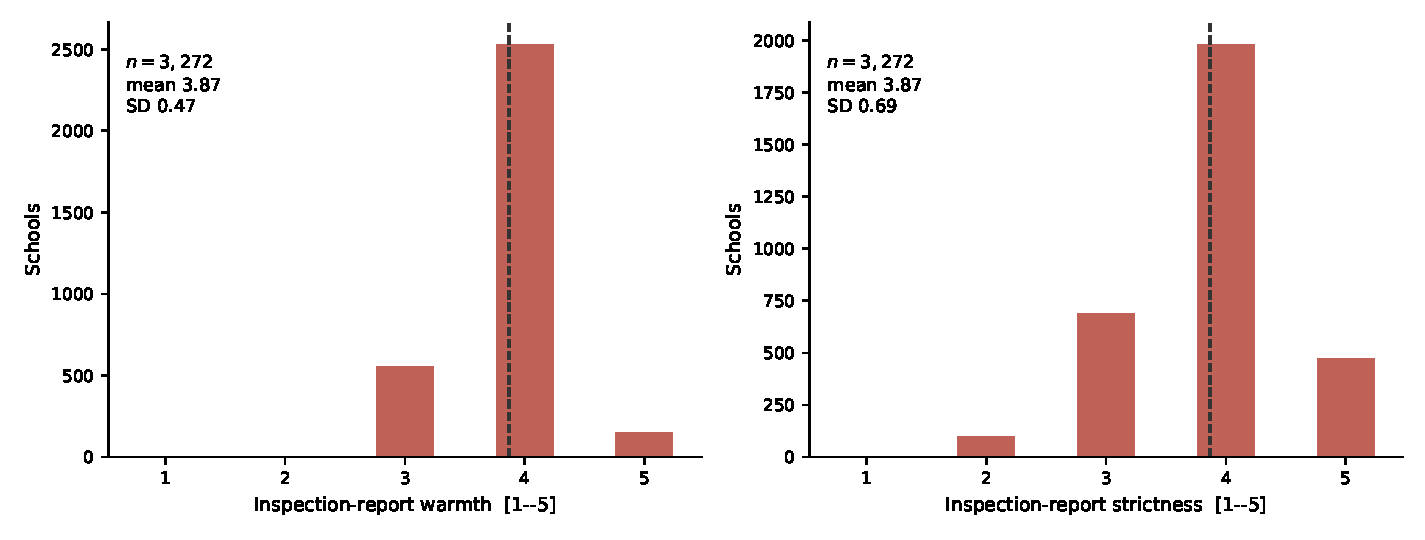
\includegraphics[width=\textwidth]{fig_A2_ofsted_distributions.pdf}
  \caption{Distributions of the inspection-report warmth (left) and strictness (right) scores
    across the national population (1--5 scale). Dashed lines mark means.
    The strictness score enters the national extension; the warmth score is
    not used as a predictor, for the reasons given in the previous chapter.}
  \label{fig:ofsted_distributions}
\end{figure}

\textbf{Controls.} All specifications condition on the same set of
controls. The first is the mean Key Stage~2 score of the cohort, which guards
against the possibility that Progress~8 is not fully neutral to intake. The
next are the shares of pupils eligible for free school meals, with English as
an additional language and with special educational needs, which are the
composition measures most strongly associated with progress. Then come log
school size; academy status, urban location and selective admissions; and
the number of years since the school's last inspection, since a school that
was inspected long ago is described by an older report. Finally, the
school's overall inspection grade as at August 2019 enters as a set of
dummies. I use the 2019 grade rather than the current one because a
contemporaneous grade is partly an outcome of the culture being measured. I
enter it at all because it is the best available summary of how the school
was regarded before the outcome cohorts arrived. Six visited schools
converted to academies after 2019 and carry no grade of their own. For five
of them the predecessor school's 2019 grade is used, and the sixth is
dropped where the control is required.

\textbf{Sample.} Two exclusions apply. The first is schools whose statutory
entry age is 13 or above (university technical colleges, studio schools and
similar; 98 schools nationally, two of them among those visited), which are
excluded from every outcome regression. Progress~8 measures progress from
age 11, and these schools enrol their pupils at 13 or 14, so their figure
attributes to them progress that was made elsewhere. The second is one
visited school that lacks the years-since-inspection control. The primary
estimation sample is therefore $n = \PrimarySpecN$. \Cref{tab:outcome_stats}
and \cref{tab:control_stats} report descriptive statistics for the outcomes
and the controls. The visited schools' mean Progress~8 is about a quarter of
a grade above zero, with a standard deviation a little below the national
one, which is the restricted range noted in the previous chapter. On the
controls the visited schools are close to the interviewed ones and to the
country as a whole: 29 per cent of pupils eligible for free school meals, 16
per cent with special educational needs, three-quarters academies, nine in
ten urban, one in twenty selective, and a 2019 grade distribution of roughly
a quarter Outstanding, five-eighths Good and one in nine below Good. The one
visible difference is the share of pupils with English as an additional
language, 28 per cent against 21 per cent in the interviewed sample, which
reflects the London weighting, and it is controlled for throughout. The
correlations between the culture scores and the controls are all below
$|0.3|$ (\cref{tab:score_controls_corr}). This means that the culture measures are not close proxies for intake or
school type, and that the coefficients below cannot simply be reflecting
differences in pupil composition.

\begin{table}[htbp]
  \centering
  \caption{Summary statistics: Progress~8 component outcomes by data tier}
  \label{tab:outcome_stats}
  \small
  \begin{tabular}{llrrrrr}
    \toprule
    Outcome & Tier & $N$ & Mean & SD & Min & Max \\
    \midrule
    \multirow{3}{*}{P8 English (2-yr avg)} & Tier~1: Visited (enacted) & 102 & 0.263 & 0.505 & -0.750 & 1.545 \\
     & Tier~2: Interview (303) & 299 & 0.092 & 0.488 & -1.485 & 1.545 \\
     & National & 3240 & -0.017 & 0.519 & -4.035 & 2.360 \\
    \addlinespace[3pt]
    \multirow{3}{*}{P8 Maths (2-yr avg)} & Tier~1: Visited (enacted) & 102 & 0.277 & 0.446 & -0.595 & 1.345 \\
     & Tier~2: Interview (303) & 299 & 0.092 & 0.473 & -1.370 & 1.345 \\
     & National & 3240 & -0.017 & 0.487 & -2.030 & 2.660 \\
    \addlinespace[3pt]
    \multirow{3}{*}{P8 EBacc (2-yr avg)} & Tier~1: Visited (enacted) & 102 & 0.307 & 0.543 & -0.790 & 1.490 \\
     & Tier~2: Interview (303) & 299 & 0.115 & 0.571 & -1.960 & 1.490 \\
     & National & 3240 & -0.020 & 0.587 & -4.950 & 2.655 \\
    \addlinespace[3pt]
    \multirow{3}{*}{P8 Open (2-yr avg)} & Tier~1: Visited (enacted) & 102 & 0.182 & 0.520 & -1.095 & 1.435 \\
     & Tier~2: Interview (303) & 299 & 0.054 & 0.556 & -3.095 & 1.500 \\
     & National & 3240 & -0.034 & 0.573 & -5.140 & 2.220 \\
    \addlinespace[3pt]
    \multirow{3}{*}{Att8 English (2024--25)} & Tier~1: Visited (enacted) & 102 & 10.685 & 1.744 & 8.000 & 17.300 \\
     & Tier~2: Interview (303) & 300 & 10.278 & 1.694 & 6.700 & 17.300 \\
     & National & 3274 & 10.049 & 1.702 & 0.100 & 17.300 \\
    \addlinespace[3pt]
    \multirow{3}{*}{Att8 Maths (2024--25)} & Tier~1: Visited (enacted) & 102 & 9.918 & 1.960 & 6.700 & 17.400 \\
     & Tier~2: Interview (303) & 300 & 9.510 & 1.899 & 5.200 & 17.400 \\
     & National & 3274 & 9.263 & 1.879 & 0.300 & 17.600 \\
    \addlinespace[3pt]
    \multirow{3}{*}{Att8 EBacc (2024--25)} & Tier~1: Visited (enacted) & 102 & 14.835 & 3.206 & 9.500 & 26.500 \\
     & Tier~2: Interview (303) & 300 & 14.157 & 3.117 & 6.200 & 26.500 \\
     & National & 3274 & 13.696 & 3.103 & 0.500 & 26.600 \\
    \addlinespace[3pt]
    \multirow{3}{*}{Att8 Open (2024--25)} & Tier~1: Visited (enacted) & 102 & 14.722 & 2.913 & 10.300 & 26.300 \\
     & Tier~2: Interview (303) & 300 & 14.189 & 2.860 & 4.900 & 26.300 \\
     & National & 3274 & 13.869 & 2.830 & 0.000 & 26.300 \\
    \bottomrule
  \end{tabular}
  \begin{minipage}{\linewidth}
    \vspace{2pt}
    \footnotesize
    \textit{Notes:} P8 outcomes are 2-year averages of 2022--23 and 2023--24 component scores where both
    years are available; single-year used where only one is present. Att8 2024--25 components are the
    contemporaneous robustness outcome; no Progress~8 is available for this cohort because the cohort were
    in Year~6 in 2019--20 when Key Stage~2 assessments were cancelled. Tier~2 is the full interviewed
    sample and therefore contains Tier~1; both are subsets of the national sample, hence the different
    $N$ values across tiers.
  \end{minipage}
\end{table}


\begin{table}[htbp]
  \centering
  \caption{Summary statistics: control variables by data tier}
  \label{tab:control_stats}
  \small
  \begin{tabular}{lrrrrrr}
    \toprule
    & \multicolumn{3}{c}{Tier~1 ($N=102$, visited)} & \multicolumn{3}{c}{Tier~2 ($N=303$, interview)} \\
    \cmidrule(lr){2-4}\cmidrule(lr){5-7}
    Variable & $N$ & Mean & SD & $N$ & Mean & SD \\
    \midrule
    \multicolumn{7}{l}{\textit{Pupil composition and prior attainment}} \\
    \quad Mean KS2 score & 102 & 104.917 & 2.909 & 300 & 104.627 & 2.714 \\
    \quad FSM eligible (\%) & 102 & 29.2 & 15.7 & 303 & 28.0 & 14.7 \\
    \quad EAL share (\%) & 102 & 27.8 & 26.2 & 300 & 21.3 & 22.2 \\
    \quad SEN share (\%) & 102 & 15.5 & 7.3 & 300 & 15.6 & 7.3 \\
    \quad Log school size & 102 & 6.964 & 0.368 & 303 & 6.938 & 0.398 \\
    \quad Yrs since Ofsted & 101 & 4.797 & 3.891 & 295 & 4.919 & 4.006 \\
    \addlinespace[3pt]
    \multicolumn{7}{l}{\textit{School characteristics (share)}} \\
    \quad Academy school & 102 & \multicolumn{2}{c}{73.5\%} & 303 & \multicolumn{2}{c}{71.6\%} \\
    \quad Urban location & 102 & \multicolumn{2}{c}{90.2\%} & 303 & \multicolumn{2}{c}{88.4\%} \\
    \quad Selective admissions & 102 & \multicolumn{2}{c}{93.1\%} & 303 & \multicolumn{2}{c}{92.4\%} \\
    \addlinespace[3pt]
    \multicolumn{7}{l}{\textit{Pre-COVID Ofsted grade (as at 31~August~2019)}} \\
    \quad Grade~1 (Outstanding) & 25 & \multicolumn{2}{c}{26.3\%} & 63 & \multicolumn{2}{c}{23.6\%} \\
    \quad Grade~2 (Good) & 59 & \multicolumn{2}{c}{62.1\%} & 170 & \multicolumn{2}{c}{63.7\%} \\
    \quad Grade~3 (Requires improvement) & 10 & \multicolumn{2}{c}{10.5\%} & 27 & \multicolumn{2}{c}{10.1\%} \\
    \quad Grade~4 (Inadequate) & 1 & \multicolumn{2}{c}{1.1\%} & 7 & \multicolumn{2}{c}{2.6\%} \\
    \quad No pre-COVID grade & 7 & & & 36 & & \\
    \bottomrule
  \end{tabular}
  \begin{minipage}{\linewidth}
    \vspace{2pt}
    \footnotesize
    \textit{Notes:} KS2 is the mean scaled score of the 2023--24 KS4 cohort at Key Stage~2.
    FSM is the share eligible for the pupil premium (FSM6 definition); EAL and SEN are KS4
    cohort shares from the 2023--24 performance tables. Pre-COVID Ofsted grade is the overall
    effectiveness grade from the Ofsted Management Information snapshot as at 31~August~2019,
    used as the primary endogeneity-safe control; the contemporary 2024 grade enters sensitivity
    analyses only. Tier~1 (102 schools) have both visit and interview data; Tier~2 (303 schools)
    includes Tier~1.
  \end{minipage}
\end{table}

As the previous chapter records, the visited schools lean towards stronger
schools than the national population, so the estimates apply most directly
to a population somewhat above the national average, and the restricted
range of both culture and outcomes works against finding associations rather
than for them.

% ============================================================
\section{Empirical Specification}
\label{sec:p2_spec}

The primary specification is
%
\begin{equation}
  \label{eq:main}
  Y_s = \alpha + \beta_W W_s + \beta_S S_s + \mathbf{X}_s'\gamma
        + \sum_g \delta_g \,\mathbb{1}[G_s = g] + \varepsilon_s ,
\end{equation}
%
where $Y_s$ is the two-year average Progress~8 (overall, English or Maths)
of school $s$, $W_s$ and $S_s$ are its enacted warmth and strictness scores
in standard-deviation units, $\mathbf{X}_s$ is the set of controls listed
above and $G_s$ is its 2019 inspection grade. Standard errors are
heteroskedasticity-consistent (HC3), which is the small-sample variant that
is appropriate when $n$ is near 100. I estimate three stages:
equation~(\ref{eq:main}); the same equation with the teaching-practice score
$T_s$ in place of $W_s$ and $S_s$; and the equation with all three. Each
dimension is also entered on its own. The national extension replaces $W_s$
and $S_s$ with the inspection-report strictness score, standardised, on all
schools with an outcome, and is estimated both with and without the grade
dummies.

The estimates are associations, and it is worth being exact about what the
design does and does not achieve. Because the outcome is value-added, the
comparison is between schools whose pupils started from the same place. This
means that the first and largest confound in any school-effects estimate,
namely that stronger schools take stronger pupils, is removed by
construction, and the Key Stage~2 control guards against what remains.
Because the culture measures come from visits that were mostly made in the
year after the outcome cohorts sat their examinations, reverse causation in
the ordinary sense, that good results produce a warm and orderly school, is
not ruled out by the timing. What the design relies on instead is that culture is persistent, so that
what was observed in 2024/25 is a reasonable measure of what the 2022/23
and 2023/24 cohorts experienced. The appendix
supports that reading in two ways. A school's Progress~8, and the structural
characteristics that shape it, are stable across years relative to the
differences between schools, and the one cohort that was measured at the
same time as the fieldwork gives coefficients within $0.05$ of the primary
ones. Because the 2019 grade is held constant, the comparison is between
schools that the inspectorate regarded alike before the outcome cohorts
arrived, so a school's reputation, and whatever that reputation draws in
terms of staff and families, is partly absorbed. Finally, because the sample excludes schools that enrol at 13 or 14, no
school is credited with progress that was made at another school.

What the design cannot do is rule out the possibility that some persistent
characteristic of a school produces both its culture and its results. This
might be a headteacher who is effective in ways that the visit does not
measure, or a stable school reputation that draws in both committed staff
and motivated families. Two features of the data bear on this without
resolving it. The teaching-practice score is observed alongside the culture
scores, so the most obvious such characteristic, that warm and orderly
schools are simply schools whose teachers teach well, can be tested directly
rather than assumed away. Secondly, the strictness result reproduces across the
national population using a text-based measure with the inspection grade
held constant, so it is not an artefact of which schools agreed to be
visited. The sorting concern that remains, which is that strict schools may
retain fewer pupils with social, emotional and mental-health needs and gain
in measured progress by that route, is tested by adding a pre-period measure
of that share. The estimates are nonetheless presented as associations
throughout, and no coefficient is described as an effect.

% ============================================================
\section{Results}
\label{sec:p2_results}

\textbf{Culture predicts progress.} \Cref{tab:spec_ladder} reports the
primary estimates. In the primary specification observed warmth has a
coefficient of $\hat{\beta}_W = \PrimarySpecW$ ($p = 0.002$) and observed
strictness a coefficient of $\hat{\beta}_S = \PrimarySpecS$ ($p = 0.007$) on
overall Progress~8, with $R^2 = 0.62$. The table shows the same equation
under four treatments of the grade control, from requiring an original 2019
grade ($n = 95$) to dropping the control altogether ($n = 100$), and the
coefficients move by less than $0.02$ across the four. Both dimensions
contribute, as the authoritative-school framework predicts, with warmth
somewhat the stronger of the two.

\begin{table}[htbp]\centering
\def\sym#1{\ifmmode^{#1}\else\(^{#1}\)\fi}
\small
\caption{The headline gold-standard model under four treatments of the pre-COVID
inspection-grade control. Each row is the same regression of average Progress 8 on
enacted warmth ($W$) and enacted strictness ($S$) with the full control set; the rows
differ only in how schools with a missing 2019 grade are handled. Schools with a
statutory admission age of 13 or above are excluded throughout.}
\label{tab:spec_ladder}
\begin{tabular}{lccc}
\toprule
Grade-control specification & $N$ & Warmth ($W$) & Strictness ($S$) \\
\midrule
Grade as recorded (missing dropped)      &  95 & 0.155\sym{***}  & 0.128\sym{***}  \\
                                         &     & (0.045)        & (0.047)        \\
\addlinespace
Predecessor-filled grade (primary)       &  99 & 0.143\sym{***}  & 0.131\sym{***}  \\
                                         &     & (0.045)        & (0.047)        \\
\addlinespace
Missing-grade category retained          & 100 & 0.143\sym{***}  & 0.131\sym{***}  \\
                                         &     & (0.045)        & (0.047)        \\
\addlinespace
No grade control                         & 100 & 0.140\sym{***}  & 0.127\sym{***}  \\
                                         &     & (0.046)        & (0.046)        \\
\bottomrule
\end{tabular}
\begin{minipage}{\linewidth}
\smallskip
\footnotesize\textit{Notes:} Standard errors in parentheses.
\sym{*} \(p<0.10\), \sym{**} \(p<0.05\), \sym{***} \(p<0.01\).
Outcome is average Progress 8; predictors are standardised. Seven visited academies
lacked a 2019 grade under their current URN; the primary specification fills five of
them from the predecessor school's grade. Including the late-entry schools leaves the
primary estimates essentially unchanged ($W = 0.139$, $p = 0.003$;
$S = 0.133$, $p = 0.006$; $N = 100$).
\end{minipage}
\end{table}


It is worth putting these magnitudes in context. A standard deviation of
enacted warmth is about one point on the ten-point scale, or half a point on
the five-point scale of every warmth item in every lesson observed. The
associated $0.15$ of a grade is about a quarter of a standard deviation of
school Progress~8 nationally. It is also about a quarter of the gap in mean
Progress~8 between schools graded Outstanding and Good in 2019 ($0.53$), and
about a quarter of the gap between the least and the most disadvantaged
quarter of schools by free-school-meal share ($0.62$). Two standard deviations on both dimensions together, which is roughly the
distance within the visited range from a school that is low on both
dimensions to one that is high on both, is associated with about half a
grade per subject per pupil. That is the size
of the difference that the performance tables treat as separating a
well-above-average school from an average one.

Entered on its own, each dimension has a coefficient of about $0.2$
(\cref{tab:univariate_ws}): $0.219$ for warmth and $0.199$ for strictness.
Entered jointly, warmth keeps two-thirds of its solo coefficient and
strictness about half. The two dimensions therefore share some variance, as
their correlation of $\CorrWarmthStrictnessEnacted$ implies, but each
contains substantial information that the other does not. This is the
empirical basis for treating them as two constructs. If there were a single
scale running from warm to strict, one coefficient would absorb the other.

\begin{table}[htbp]\centering
\def\sym#1{\ifmmode^{#1}\else\(^{#1}\)\fi}
\small
\caption{Warmth and strictness entered alone and together. Each column is a Progress 8
outcome; the first two rows enter one culture dimension at a time and the final two
rows enter both jointly, always with the full control set and the predecessor-filled
grade control. The drop from the univariate to the joint coefficients shows the two
dimensions share some variance, but each keeps an independent association when the
other is held fixed.}
\label{tab:univariate_ws}
\begin{tabular}{llccc}
\toprule
Specification & Term & Overall & English & Maths \\
\midrule
$S$ only   & Strictness ($S$) & 0.195\sym{***} & 0.170\sym{***} & 0.156\sym{***} \\
           &                  & (0.033)        & (0.039)        & (0.033)        \\
\addlinespace
$W$ only   & Warmth ($W$)     & 0.206\sym{***} & 0.207\sym{***} & 0.164\sym{***} \\
           &                  & (0.035)        & (0.037)        & (0.039)        \\
\midrule
Joint      & Warmth ($W$)     & 0.132\sym{***} & 0.158\sym{***} & 0.104\sym{**}  \\
           &                  & (0.042)        & (0.041)        & (0.050)        \\
\addlinespace
Joint      & Strictness ($S$) & 0.117\sym{***} & 0.077\sym{*}   & 0.095\sym{**}  \\
           &                  & (0.039)        & (0.042)        & (0.042)        \\
\midrule
$N$        &                  & 100            & 100            & 100            \\
\bottomrule
\end{tabular}
\begin{minipage}{\linewidth}
\smallskip
\footnotesize\textit{Notes:} Standard errors in parentheses.
\sym{*} \(p<0.10\), \sym{**} \(p<0.05\), \sym{***} \(p<0.01\).
Gold-standard visited tier, late-entry schools excluded. EBacc and Open components
are reported in the chapter appendix.
\end{minipage}
\end{table}


At the level of the components, warmth is significant for both subjects (English
$0.162$, $p < 0.001$; Maths $0.135$, $p = 0.011$), while strictness falls
short of significance in each taken alone (English $0.071$, $p = 0.11$;
Maths $0.076$, $p = 0.09$), so that its association with overall progress
is the sum of two parts with the same sign. Estimates for the two remaining
components, and the analysis of subject entry that they require, are in
\cref{app:3A:tables}.

\textbf{Teaching quality does not account for it.} \Cref{tab:stages23_trio}
reports the second and third stages. On its own, the visit's
teaching-practice score predicts overall Progress~8 at $0.206$ ($p <
0.001$), but with a lower $R^2$ ($0.55$) than the two culture scores. When it
is added to the primary specification it enters at $0.015$ ($p = 0.82$), and
the culture coefficients are unchanged ($0.137$ and $0.103$).

There are two possible readings of this result, and the data do not allow
a choice between them. The first reading is that culture and instruction
are distinct predictors of progress. On this reading, what a school is like
between and around lessons, and how orderly its lessons are, matter over and
above how well the lessons are taught, and the culture association is not
simply the teaching-quality association under another name. The second
reading is that the teaching score is the noisiest of the three visit
measures, because it is built from ten items on which the observers agree
least, and that its signal is absorbed by the two culture scores with which
it is correlated. On this reading the null result on teaching understates
what instruction contributes. Three facts favour the first reading, although
they do not settle the matter. Firstly, the teaching score on its own
predicts progress well, so it is clearly not just noise. Secondly, the
culture coefficients do not move at all when it enters, whereas if
absorption were taking place one would expect to see movement in both
directions. Thirdly, the culture association runs partly through
out-of-lesson warmth, which no measure of classroom teaching could pick up.
What would separate the two readings is a measure of teaching quality that
is independent of the visit, and no such measure exists for these schools.
The claim I make is therefore the narrower one, which is that conditioning
on observed teaching quality does not account for the culture association.

\begin{table}[htbp]
\centering
\small
\caption{Stages 2 and 3 under the primary specification: teaching quality as
the sole culture predictor (Stage~2), and teaching quality added to the
warmth-and-strictness model (Stage~3). Coefficients are per standard
deviation of the predictor; HC3 robust standard errors; $n = 100$. The full
five-outcome versions, estimated on the previous specification, are reported
in the appendix.}
\label{tab:stages23_trio}
\begin{tabular}{lccc}
\toprule
 & \textit{Overall P8} & \textit{English} & \textit{Maths} \\
\midrule
\multicolumn{4}{l}{\textit{Stage 2: teaching quality only}} \\
\addlinespace[2pt]
Teaching $T$ & 0.202\sym{***} & 0.184\sym{***} & 0.159\sym{***} \\
             & (0.000) & (0.000) & (0.001) \\
$R^2$        & 0.562 & 0.560 & 0.484 \\
\addlinespace[6pt]
\multicolumn{4}{l}{\textit{Stage 3: warmth, strictness and teaching}} \\
\addlinespace[2pt]
Warmth $W$   & 0.121\sym{*}  & 0.165\sym{**} & 0.098 \\
             & (0.033) & (0.006) & (0.108) \\
Strictness $S$ & 0.113\sym{**} & 0.080 & 0.093\sym{*} \\
             & (0.005) & (0.064) & (0.047) \\
Teaching $T$ & 0.020 & $-$0.010 & 0.011 \\
             & (0.758) & (0.879) & (0.872) \\
\bottomrule
\end{tabular}
\begin{minipage}{0.8\linewidth}
\vspace{4pt}\scriptsize
\textit{Notes}: $p$-values in parentheses. \sym{*} $p<0.05$, \sym{**}
$p<0.01$, \sym{***} $p<0.001$. Primary specification throughout: full
control set, predecessor-filled pre-COVID grade, late-entry schools
excluded.
\end{minipage}
\end{table}


\textbf{The dimensions add.} \Cref{fig:quadrant_ws} plots the visited
schools by their two culture scores, shaded by progress. Schools in the warm
and strict quadrant are predominantly above-average performers, and the
other three quadrants are all populated, which is what makes it possible to
test the combination. Formally, the warm-and-strict quadrant sits $0.40$ of
a grade above the rest of the sample after controls ($p < 0.001$), while the
interaction between the two standardised scores is zero ($0.038$, $p =
0.27$; \cref{tab:robustness_overall}). In other words, warmth and strictness
add to one another rather than amplifying each other. The best schools have
both because each of them helps, and not because of any combination effect,
and a school that is strong on one dimension still gains from the other. Breaking
the visit scores down into their five observational blocks
(\cref{tab:subscores}) shows that the association runs through warmth
outside lessons and orderly conduct within them. Out-of-lesson warmth
($0.111$, $p = 0.006$) and in-lesson strictness ($0.115$, $p = 0.008$)
survive joint entry, and their counterparts do not. This means that the
relational quality that goes with progress is the one visible in corridors
and at break, and the order that goes with it is the one visible in lessons.

\begin{figure}[htbp]
  \centering
  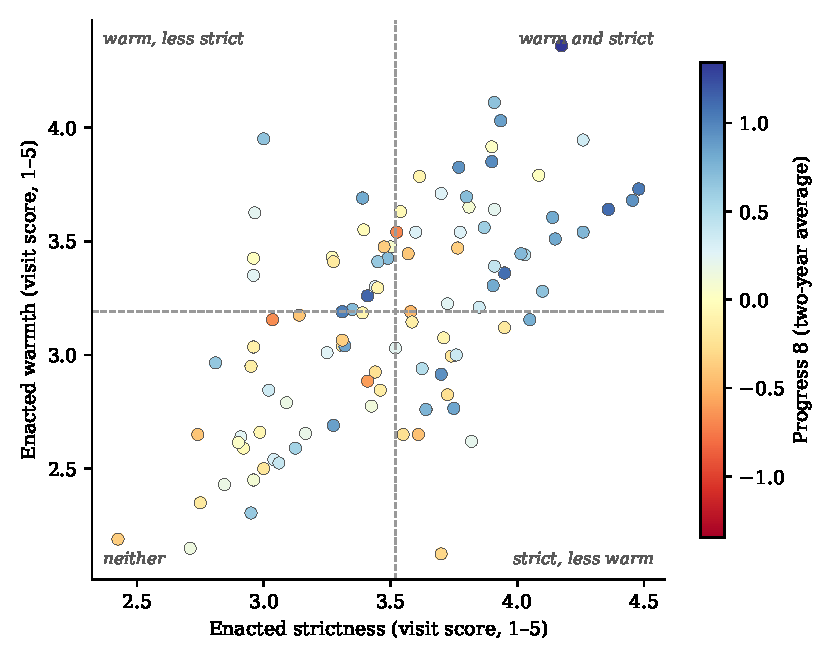
\includegraphics[width=0.85\textwidth]{fig_quadrant_ws.pdf}
  \caption{Enacted warmth and strictness for the visited schools, shaded by
  Progress~8 (two-year average). Dashed lines mark sample medians. The
  adjusted quadrant comparison is in \cref{tab:typology}.}
  \label{fig:quadrant_ws}
\end{figure}

\textbf{Espoused culture does not predict progress.} Substituting the
headteacher's espoused scores for the observed ones on the same schools
reduces the warmth coefficient to $0.051$ ($p = 0.29$), while espoused
strictness retains an association of the same size as the observed one
($0.120$, $p = 0.018$). The asymmetry found in the previous chapter's measurement appears again
here in prediction. What a headteacher says about warmth contains no
information about progress, and what they say about behaviour systems
contains some. This is the pattern that the previous chapter's
finding predicts, since espoused warmth was shown there to be only weakly
related to observed warmth, and espoused strictness more closely related to
observed strictness. It is also a check on the observed measures as much as
on the espoused ones. Had the espoused scores predicted progress as well as
the observed ones, the visits would have added nothing that an hour with the
headteacher could not supply. Two related results are in
\cref{app:3A:tables}. The gap between a school's espoused and enacted scores
predicts nothing beyond the enacted level, and the association is not
confined to the visited schools' own report on themselves, since parents'
survey responses on their children's happiness and safety are positively
associated with progress ($0.14$ per standard deviation), with the caveat
that satisfaction and results are jointly determined.

\textbf{National extension.} The inspection-report strictness score, which
the previous chapter showed to track observed strictness at $r =
\CorrOfstedStrictness$, is available for \NNationalStrictness{} schools with
an outcome, which is some thirty times the size of the visited sample. On
the full control set without the grade it has a coefficient of
$\BetaNationalStrictness$ ($p < 0.001$, $R^2 = 0.52$;
\cref{tab:national_strictness}). With the 2019 grade added ($n = 2{,}746$)
the coefficient is $0.140$, and no component estimate moves by more than
$0.005$. Two things follow from this. The first concerns
the score itself. A score read from an inspection report might be thought to be a proxy for
the inspectorate's overall approval, in which case the association would
really be the grade's association. However, the coefficient is unchanged by
conditioning on the grade, and a proxy for the grade would lose most of its
coefficient when the grade entered. The score therefore captures what the
report says about conduct and enforcement over and above the verdict, and
it is this that predicts progress. The second concerns the visited
sample. The visited schools agreed to be visited, and the previous chapter
showed that they lean towards stronger schools. The national coefficient is
estimated on every school with a report and an outcome, and it is of the
same order as the visited strictness coefficient in standard-deviation
units, if anything larger. The strictness result is therefore not a property
of the schools that agreed to take part. What the extension does not provide
is the same reassurance for warmth, since no text source contains observed
warmth, and nor does it provide identification, since a text-derived measure
is open to the same omitted-variable concern as an observed one. Two further text-derived
results are consistent with the previous chapter's measurement findings and
are reported in \cref{tab:llm_p8_matrix}: the behaviour-policy warmth score
is significantly \emph{negatively} associated with progress, and the website
warmth and strictness scores are not associated with it at all.

\begin{table}[htbp]\centering
\def\sym#1{\ifmmode^{#1}\else\(^{#1}\)\fi}
\caption{National extension: Ofsted LLM strictness and Progress~8}
\label{tab:national_strictness}
\resizebox{\textwidth}{!}{%
\begin{tabular}{l*{5}{c}}
\toprule
 & Overall & English & Maths & EBaC & Open \\
\midrule
\multicolumn{6}{l}{\textit{Panel A: published specification (Ofsted grade omitted)}} \\
Strictness (Ofsted LLM, 1--5 scale) & 0.166\sym{***} & 0.152\sym{***} & 0.142\sym{***} & 0.171\sym{***} & 0.190\sym{***} \\
 & (0.008) & (0.009) & (0.008) & (0.010) & (0.010) \\
$N$ & 3{,}147 & 3{,}147 & 3{,}147 & 3{,}147 & 3{,}147 \\
$R^2$ & 0.522 & 0.455 & 0.471 & 0.499 & 0.423 \\
\addlinespace[6pt]
\multicolumn{6}{l}{\textit{Panel B: adding the pre-COVID (2019) Ofsted grade}} \\
Strictness (Ofsted LLM, 1--5 scale) & 0.167\sym{***} & 0.154\sym{***} & 0.143\sym{***} & 0.174\sym{***} & 0.190\sym{***} \\
 & (0.009) & (0.009) & (0.009) & (0.011) & (0.010) \\
$N$ & 2{,}823 & 2{,}823 & 2{,}823 & 2{,}823 & 2{,}823 \\
$R^2$ & 0.534 & 0.463 & 0.477 & 0.510 & 0.435 \\
\bottomrule
\end{tabular}%
}
\begin{minipage}{\linewidth}
  \vspace{4pt}
  \footnotesize
  \textit{Notes:} Heteroskedasticity-robust (HC3) standard errors in
  parentheses. \sym{*} \(p<0.10\), \sym{**} \(p<0.05\), \sym{***} \(p<0.01\).
  All specifications control for prior attainment (KS2), FSM, EAL, SEN, log
  cohort size, years since inspection, academy status, urban location and
  selective status. Panel~A is the specification reported in the text, which
  omits the Ofsted grade because the strictness score is read from the same
  inspection report. Panel~A includes 3{,}147 schools. Panel~B adds the pre-COVID
  (2019) overall Ofsted grade as a set of dummies---the same control used in
  the primary Tier~1 specification---and is estimated on the 2{,}823 schools with
  a 2019 grade on record, 324 fewer than Panel~A. The strictness
  coefficient is materially unchanged throughout, indicating that it is not
  simply recording Ofsted's overall approval of the school.
\end{minipage}
\end{table}


\textbf{Robustness.} \Cref{tab:robustness_overall} reports the primary
estimate under alternative specifications, all on the primary sample, and
each of them addresses a particular doubt. The grade control might be doing
the work, or absorbing part of it. Dropping it leaves $0.153$ and $0.097$
($n = 100$). Averaging two cohorts might smooth over a result that holds in
only one of them. The single 2023/24 outcome year gives $0.155$ and $0.105$.
Strict schools might have fewer pupils with social, emotional and
mental-health needs, and gain in measured progress by that route. Adding the
2015/16 baseline share of such pupils, which was measured before any of the
culture was observed, gives $0.149$ and $0.090$ ($n = 94$), and the sorting
channel accounts for under a tenth of the strictness association
(\cref{tab:semh_mechanism}). Progress~8 might be peculiar. On the 2024/25
cohort's Attainment~8, which does not condition on intake, both dimensions
remain significant, both on the total of the four buckets ($1.40$, $1.32$
points) and on the English bucket alone ($0.35$, $0.16$, the last at $p =
0.12$).
The enacted scores might reflect something about the visits themselves. About
a third of the observed lessons were rated by one researcher rather than
two, those lessons were scored a little lower, and the share of such lessons
in a school's visit correlates $-0.25$ with its warmth score. Adding that
share as a control moves nothing ($0.150$ and $0.105$; the share itself
has a coefficient of $0.03$, $p = 0.76$). Restricting the sample to the 64 schools in
which every lesson was rated by two researchers gives $0.189$ for warmth
($p = 0.001$) and $0.071$ for strictness ($p = 0.15$). The warmth estimate is
larger on that subset and the strictness estimate smaller, with a standard
error a third larger on two-thirds of the sample, so the strictness result
is the one that depends on the full sample. All but the English-bucket and
the double-rated strictness cells leave both coefficients significant at the
five per cent level or better.

Two further checks concern timing and the headteacher. Within-school
Progress~8 is stable across years (the mean within-school standard deviation
is $0.20$, against a between-school standard deviation of about $0.5$),
which supports using culture measured after the outcome window as a proxy
for culture during it (\cref{tab:stability_p8}), and the 2024/25
pseudo-progress measure, which is the one cohort measured at the same time
as the fieldwork, gives coefficients within $0.05$ of their real-Progress~8
counterparts (\cref{tab:p8_proxy}). Restricting the sample to the 22 schools
whose headteacher is confirmed as unchanged since the last inspection, so
that the culture observed is the culture the outcome cohorts had, leaves the
strictness point estimates at or above the full-sample values and the warmth
estimates imprecise. That subsample is too small to be informative either
way (\cref{app:3A:tables}).

\begin{table}[htbp]\centering
\def\sym#1{\ifmmode^{#1}\else\(^{#1}\)\fi}
\caption{Robustness: Overall Progress 8}
\label{tab:robustness_overall}
\resizebox{\textwidth}{!}{%
\begin{tabular}{l*{6}{c}}
\toprule
                    &\multicolumn{1}{c}{(1)}&\multicolumn{1}{c}{(2)}&\multicolumn{1}{c}{(3)}&\multicolumn{1}{c}{(4)}&\multicolumn{1}{c}{(5)}&\multicolumn{1}{c}{(6)}\\
                    &\multicolumn{1}{c}{Primary}&\multicolumn{1}{c}{No grade}&\multicolumn{1}{c}{2023-24}&\multicolumn{1}{c}{Att8 2425}&\multicolumn{1}{c}{W$\times$S}&\multicolumn{1}{c}{SEMH ctrl}\\
\midrule
$W$                 &       0.127\sym{***}&       0.142\sym{***}&       0.138\sym{***}&       0.895\sym{*}  &      -0.106         &       0.130\sym{***}\\
                    &     (0.045)         &     (0.045)         &     (0.049)         &     (0.502)         &     (0.294)         &     (0.044)         \\
\addlinespace
$S$                 &       0.120\sym{**} &       0.099\sym{**} &       0.119\sym{**} &       1.767\sym{***}&      -0.099         &       0.114\sym{***}\\
                    &     (0.047)         &     (0.044)         &     (0.047)         &     (0.476)         &     (0.270)         &     (0.041)         \\
\midrule
N                   &          95         &         101         &          95         &          95         &          95         &          90         \\
r2                  &       0.595         &       0.568         &       0.601         &       0.883         &       0.599         &       0.638         \\
\bottomrule
\multicolumn{7}{l}{\footnotesize Standard errors in parentheses}\\
\multicolumn{7}{l}{\footnotesize \sym{*} \(p<0.10\), \sym{**} \(p<0.05\), \sym{***} \(p<0.01\)}\\
\end{tabular}%
}
\end{table}


\textbf{Implications.} Two implications bear on the current policy debate,
and they follow from the pattern of results rather than from any single
coefficient. The behaviour debate treats discipline as the part of school improvement
that does the work, and relational culture as secondary. These estimates
give relational culture at least the weight of discipline, they show no
trade-off between the two, and they place the warm-and-strict schools
two-fifths of a grade ahead. On these estimates, a school that tightens its
behaviour systems but lets relationships slip loses about as much as it
gains.
The second implication is that the association runs through relational
quality outside lessons and orderly conduct within them. This places the relational work that matters outside the classroom, in
corridors, at break and at the gate, which is where schools currently direct
the least observation and training effort. Both implications are conditional on the association being at
least partly causal, which the design supports but does not establish.

% ============================================================
\section{Conclusion}
\label{sec:p2_conclusion}

Observed school culture predicts pupil progress. Across the \NTierOne{}
English secondary schools that were visited, a standard deviation of
observed warmth is associated with Progress~8 that is $0.15$ of a grade
higher, and a standard deviation of observed strictness with $0.11$ of a
grade. These are significant at the one and five per cent levels
respectively, and both are stable across every reasonable specification.
The two dimensions contribute additively, with warmth somewhat the stronger,
and the schools that combine them outperform the rest by two-fifths of a
grade. Observed teaching quality does not account for the association. The
headteacher's own account of the school predicts nothing on warmth, and the
strictness score read from inspection reports reproduces the strictness
result nationally with the inspection grade held constant.

Against the literature the paper sits in, the results say three things. To
the school-effects tradition, they give a quantitative reading of two of the
correlates of ethos that Rutter and the effective-schools syntheses named,
measured by observation across a national population rather than in a
case-study sample. To the charter and academy literature, they say that the
two halves of the practice bundle, structure and support, each matter
when they are measured apart, and that neither is the whole of the effect.
To the authoritative-school literature, they supply the
academic-progress outcome that it has mostly lacked, and they find what the
typology predicts: both dimensions matter, and the schools with both do best.

The estimates are associations. They are strengthened by a value-added
outcome, by the ordering in time, by a rich set of controls and by their
stability across specifications, but they are not identified: a persistent
characteristic that produces both a school's culture and its results cannot
be ruled out with cross-sectional data. The visited sample is small and leans towards stronger schools, culture
was measured after the outcome window for most schools, and a single visit
measures a school with considerable error. A longitudinal design, with
culture observed before the outcome cohort arrived and again afterwards,
would provide evidence on the direction of the association, and a design
that observed culture changing within schools, as headteachers changed or
behaviour systems were introduced, would provide evidence on its cause. Within the
present limits, the results identify the relational and disciplinary
features of a school that go together with its pupils' progress, and they
show that one of the two, strictness, can be read at national scale from the
public record.

% ===============================================================
%  APPENDIX 3A
% ===============================================================
\clearpage
\startchapterappendix{3}
\begin{center}
  {\LARGE\bfseries Appendix to Chapter 3}\\[6pt]
  \rule{0.5\linewidth}{0.4pt}
\end{center}
\medskip
\noindent This appendix collects the supporting material for the analyses
reported in the chapter. It explains how the Progress~8 measures and the
subject entry rates are calculated, sets out the evidence on the stability of
school characteristics that underpins the choice of outcome years, and gives
the full five-outcome versions of the main results tables (the chapter body
reports overall, English and Maths Progress~8, and the EBaC and Open
components appear here) together with the secondary and exploratory
analyses.
\medskip

% - - - - - - - - - - - - - - - - - - - - - - - - - - - - - - -
\section{How the Progress 8 Measures Are Calculated}
\label{app:3A:p8mechanics}

Progress~8 measures the progress a pupil makes between the end of primary
school and GCSE, relative to pupils nationally who started from the same
point. Each pupil's GCSE results are counted across eight slots, their
attainment is compared with the national average attainment of pupils with
the same Key Stage~2 starting point, and the difference is averaged across
the school. A school at zero is exactly average; a school at $+0.5$ achieves
half a grade more per subject per pupil than would be expected from its
intake.

The eight slots are structured, and this structure is why the thesis
treats the components differently. English and Maths each fill two slots and
are double-weighted. Every pupil sits both, so these components measure
progress and nothing else. The EBaC component covers three slots that must be filled
from a restricted academic list: sciences, computer science, history,
geography, and modern foreign languages. The Open component covers the final
three slots, which may be filled by any approved qualification, including
arts and vocational subjects. For these last six slots the school makes
entry decisions, and an unfilled slot contributes zero progress to the
school's average. Consequently, a school's EBaC and Open components mix two
different things: how much progress pupils make in the subjects they enter,
and which subjects the school enters them for. A school that enters few
pupils for languages will carry empty EBaC slots and a depressed EBaC
component even if the pupils it does enter progress well.

This structure generates a theoretical prediction about warmth and
strictness. Schools higher on strictness, characterised by structured
behaviour management, high academic expectations, and intensive pupil
steering, are more likely to direct pupils into the EBaC pathway, and could
therefore raise their EBaC component through the entry-rate channel as well
as through progress itself. Schools higher on warmth might generate stronger
progress in the more elective Open component. The five-outcome versions of the main results tables in this appendix
provide evidence on that prediction, and the entry-rate analysis below
addresses the pathway channel directly.

The entry rates themselves are calculated from the pupil count columns of
the 2023--24 performance tables, because the Department for Education
stopped publishing entry rates in percentage form in recent releases. The
EBaC entry rate is the number of pupils entered for the full EBaC suite
divided by the number of pupils at the end of Key Stage~4, and the
humanities and languages rates are constructed in the same way from their
respective counts. Entry rates are available only at the subject-group
level; individual subjects within a group cannot be distinguished in the
data collected for this project.

% - - - - - - - - - - - - - - - - - - - - - - - - - - - - - - -
\section{Structural Stability of School Characteristics}
\label{app:3A:stability}

The intra-class correlation (ICC) decomposes total variance in a panel variable
into a between-school component and a within-school over-time component. An ICC
close to one indicates that schools are much more different from each other
than they are from their own past selves. In other words, year-on-year
fluctuation within a school is small relative to the persistent differences
between schools. ICC is estimated by
one-way random-effects ANOVA on the school-year panel, retaining only schools
with at least three years of non-missing data for the variable in question.

\Cref{tab:structural_stability} reports ICC estimates and mean absolute
year-on-year changes for nine panel variables covering pupil intake composition,
special educational needs prevalence, prior attainment, pupil progress, and
per-pupil expenditure. Six of nine variables exceed ICC~$= 0.69$; all
exceed~$0.49$. Intake characteristics (the share of pupils with English as
an Additional Language, school roll, and the mean KS2 prior attainment of the
entering cohort) are especially stable, with ICC values between 0.81 and 0.92
and small mean absolute year-on-year changes relative to their between-school
spread.
Special educational needs prevalence (EHC plan share, ICC~$= 0.67$; SEN support
share, ICC~$= 0.65$) and school-level Progress~8 (ICC~$= 0.73$) show moderate to
high stability. Per-pupil expenditure, at ICC~$= 0.52$, is the most volatile, which
reflects its sensitivity to changes in national funding policy. Even so, the
majority of the variation in expenditure is between schools rather than
within schools over time.

These patterns are consistent with the view that schools occupy relatively
persistent positions in the distribution of structural characteristics, and
support the use of culture scores measured in 2024--25 as proxies for the
organisational conditions present during the 2023--24 outcome period.

The same analysis at the level of the thirteen primary-need categories
within the SEN population shows moderate stability for the Social, Emotional
and Mental Health (SEMH) category (ICC~$= 0.545$), which supports the
baseline SEMH share entering as an additional control in the robustness
specification of \cref{tab:robustness_overall}. The lower stability of SEMH
relative to the aggregate SEN support share (ICC~$= 0.65$) is consistent
with SEMH composition being partly responsive to school behaviour and
exclusion practices, rather than being determined solely by fixed intake
characteristics.

\begin{table}[htb]

\centering\small
\begin{tabular}{lrrrr}
\toprule
Variable & \multicolumn{1}{c}{Schools} & \multicolumn{1}{c}{Mean yrs}  & \multicolumn{1}{c}{ICC} & \multicolumn{1}{c}{Mean YoY} \\
\midrule
EAL share (\%)  & {3,286} & 7.7 & 0.922 & 3.7 pp \\
Pupils on roll  & {3,363} & 9.8 & 0.920 & 37 pupils \\
KS2 scaled score (2021--24)  & {3,215} & 3.0 & 0.910 & 0.86 pts \\
KS2 APS (2015--19)  & {3,100} & 4.0 & 0.812 & 0.65 pts \\
FSM share (\%)  & {3,363} & 8.8 & 0.742 & 2.3 pp \\
Progress~8  & {3,256} & 6.8 & 0.727 & 0.21 pts \\
EHC plan share (\%)  & {3,355} & 9.6 & 0.669 & 0.4 pp \\
SEN support share (\%)  & {3,361} & 9.8 & 0.653 & 1.9 pp \\
Per-pupil expenditure  & {3,331} & 6.7 & 0.516 & \pounds599 \\
\bottomrule
\end{tabular}
\caption{Structural stability of school characteristics}
\label{tab:structural_stability}
\begin{minipage}{\linewidth}
\smallskip
\footnotesize\textit{Notes:} The panel covers 2015--16 to 2024--25. ICC = intra-class correlation = between-school
variance / (between-school + within-school variance), estimated via one-way
random-effects ANOVA on the school-year panel; schools with fewer than three
years of non-missing data are excluded. \textit{Mean yrs}: mean number of
academic years of non-missing data per school. \textit{Mean YoY}: mean
absolute year-on-year change per school. EAL = English as an Additional
Language; FSM = free school meals (school census); EHC = Education, Health and
Care plan; SEN = special educational needs. The two KS2 measures use different scales from successive assessment frameworks and are therefore reported separately; no KS4 performance data
were published for 2019--20 or 2020--21 owing to the suspension of national
examinations. Progress~8 is nationally standardised with a mean near zero;
the mean YoY figure is an absolute change, not a percentage.
Per-pupil expenditure combines Consistent Financial Reporting (maintained
schools) and Academies Accounts Return (academies); the 2015--16 and 2024--25 expenditure data are incomplete.
\end{minipage}
\end{table}

\Cref{tab:p8_component_stability} reports ICC estimates separately for the four
Progress~8 components that serve as the primary outcomes of this chapter.
Among the Progress~8 components,
stability varies from ICC~$= 0.587$ for the Open component to ICC~$= 0.748$
for EBaC, with English and Maths sitting between these at ICC~$\approx 0.67$.
The higher stability of EBaC relative to Open reflects the fact that
curriculum-pathway decisions, that is, which subjects pupils are entered for,
are governed by stable school policy and change little from year to year,
while the more varied Open bucket (arts, vocational and additional GCSEs) is
subject to greater annual variation in subject mix. All four P8 components
exceed the per-pupil expenditure ICC of~$0.52$, which is the weakest result
in the main stability table; the cross-sectional design is therefore at least
as defensible for each component individually as for the structural
characteristics already discussed.

The theoretical prediction of this chapter is that warmth is most strongly
associated with the Open component, which is the dimension most sensitive to
breadth of provision and pupil engagement, and that strictness is most
strongly associated with the EBaC component, which is the dimension most
sensitive to academic pathway steering. The lower stability of Open P8 relative to EBaC P8
(ICC~$= 0.587$ versus $0.748$) implies that the warmth coefficient will be
estimated against a noisier outcome, which may attenuate the estimated effect.
This is a limitation to acknowledge in interpreting any differential finding
between components.

\begin{table}[htb]
\centering\small
\begin{tabular}{lrrrr}
\toprule
Variable & \multicolumn{1}{c}{Schools} & \multicolumn{1}{c}{Mean yrs} & \multicolumn{1}{c}{ICC} & \multicolumn{1}{c}{Mean YoY} \\
\midrule
\quad English   & {3,256} & 6.8 & 0.666 & 0.250 pts \\
\quad Maths     & {3,256} & 6.8 & 0.667 & 0.225 pts \\
\quad EBacc     & {3,256} & 6.8 & 0.748 & 0.243 pts \\
\quad Open      & {3,256} & 6.8 & 0.587 & 0.304 pts \\
\quad Overall   & {3,256} & 6.8 & 0.727 & 0.210 pts \\
\bottomrule
\end{tabular}
\caption{Structural stability of the Progress~8 components}
\label{tab:p8_component_stability}
\begin{minipage}{\linewidth}
\smallskip
\footnotesize\textit{Notes:} ICC and mean years are defined as in
\cref{tab:structural_stability}. The panel covers 2015--16 to 2023--24,
excluding 2019--20 and 2020--21, for which no KS4 performance data were
published owing to the suspension of national examinations. The components
are English (two slots, double-weighted), Maths (two slots,
double-weighted), EBacc (sciences, computer science, history, geography, and
modern foreign languages), and Open (any additional approved
qualification).
\end{minipage}
\end{table}


% - - - - - - - - - - - - - - - - - - - - - - - - - - - - - - -
\section{Additional Tables}
\label{app:3A:tables}

\Cref{tab:main_results_s1,tab:main_results_s2,tab:main_results_s3} report the
full five-outcome versions of the three main-body stages, including the EBaC
and Open components. These tables use the primary specification ($n = 99$,
predecessor-filled pre-COVID grades, late-entry schools excluded), which is
the same one as the main-body tables, so the Overall, English and Maths
columns reproduce the body exactly and the two extra columns can be read on
the same footing.
Reading the EBaC and Open columns, warmth and strictness are both
significant for EBaC with near-equal magnitudes, and both are significant for
Open as well, again with near-equal magnitudes. As \cref{app:3A:p8mechanics} explains, both components mix progress with
the school's entry decisions, so the entry-rate analysis in
\cref{tab:entry_rates} is the clearer way to answer the pathway question.
The strictness score predicts EBacc, humanities and languages entry
nationally with the inspection grade held constant, but controlling for
EBacc entry attenuates the strictness--EBaC association by only 11 to
14~per~cent. This means that most of that association is progress within
subjects rather than curriculum steering.

\begin{table}[htbp]\centering
\def\sym#1{\ifmmode^{#1}\else\(^{#1}\)\fi}
\caption{Stage 1: Total culture effect ($W + S$). Primary specification: full control set,
predecessor-filled pre-COVID inspection grade, late-entry schools excluded ---
identical to the trio reported in the chapter body, extended to all five
Progress~8 components.}
\label{tab:main_results_s1}
\resizebox{\textwidth}{!}{%
\begin{tabular}{l*{5}{c}}
\toprule
                    &     Overall         &     English         &       Maths         &        EBaC         &        Open         \\
\midrule
Warmth ($W$)        &       0.143\sym{***}&       0.167\sym{***}&       0.112\sym{**} &       0.160\sym{***}&       0.136\sym{**} \\
                    &     (0.045)         &     (0.043)         &     (0.054)         &     (0.057)         &     (0.061)         \\
\addlinespace
Strictness ($S$)    &       0.131\sym{***}&       0.087\sym{*}  &       0.110\sym{**} &       0.169\sym{***}&       0.139\sym{**} \\
                    &     (0.047)         &     (0.049)         &     (0.051)         &     (0.058)         &     (0.066)         \\
\midrule
$N$                 &          99         &          99         &          99         &          99         &          99         \\
$R^2$               &       0.624         &       0.621         &       0.527         &       0.596         &       0.518         \\
\bottomrule
\multicolumn{6}{l}{\footnotesize Standard errors in parentheses}\\
\multicolumn{6}{l}{\footnotesize \sym{*} \(p<0.10\), \sym{**} \(p<0.05\), \sym{***} \(p<0.01\)}\\
\end{tabular}%
}
\end{table}

\begin{table}[htbp]\centering
\def\sym#1{\ifmmode^{#1}\else\(^{#1}\)\fi}
\caption{Stage 2: Teaching quality benchmark ($T$)}
\label{tab:main_results_s2}
\resizebox{\textwidth}{!}{%
\begin{tabular}{l*{5}{c}}
\toprule
                    &     Overall         &     English         &       Maths         &        EBaC         &        Open         \\
\midrule
Teaching quality ($T$)&       0.251\sym{***}&       0.232\sym{***}&       0.205\sym{***}&       0.281\sym{***}&       0.274\sym{***}\\
                    &     (0.052)         &     (0.053)         &     (0.060)         &     (0.066)         &     (0.058)         \\
\midrule
$N$                 &          96         &          96         &          96         &          96         &          96         \\
$R^2$               &       0.579         &       0.571         &       0.489         &       0.522         &       0.527         \\
\bottomrule
\multicolumn{6}{l}{\footnotesize Standard errors in parentheses}\\
\multicolumn{6}{l}{\footnotesize \sym{*} \(p<0.10\), \sym{**} \(p<0.05\), \sym{***} \(p<0.01\)}\\
\end{tabular}%
}
\end{table}

\begin{table}[htbp]\centering
\def\sym#1{\ifmmode^{#1}\else\(^{#1}\)\fi}
\caption{Stage 3: Culture net of teaching ($W + S + T$). Primary specification: full control set,
predecessor-filled pre-COVID inspection grade, late-entry schools excluded ---
identical to the trio reported in the chapter body, extended to all five
Progress~8 components.}
\label{tab:main_results_s3}
\resizebox{\textwidth}{!}{%
\begin{tabular}{l*{5}{c}}
\toprule
                    &     Overall         &     English         &       Maths         &        EBaC         &        Open         \\
\midrule
Warmth ($W$)        &       0.130\sym{**} &       0.172\sym{***}&       0.103         &       0.170\sym{**} &       0.085         \\
                    &     (0.061)         &     (0.063)         &     (0.065)         &     (0.077)         &     (0.075)         \\
\addlinespace
Strictness ($S$)    &       0.110\sym{***}&       0.078\sym{*}  &       0.092\sym{*}  &       0.152\sym{***}&       0.102\sym{*}  \\
                    &     (0.041)         &     (0.044)         &     (0.049)         &     (0.052)         &     (0.057)         \\
\addlinespace
Teaching quality ($T$)&       0.020         &      -0.011         &       0.014         &      -0.021         &       0.086         \\
                    &     (0.064)         &     (0.068)         &     (0.073)         &     (0.078)         &     (0.083)         \\
\midrule
$N$                 &          99         &          99         &          99         &          99         &          99         \\
$R^2$               &       0.624         &       0.621         &       0.527         &       0.596         &       0.526         \\
\bottomrule
\multicolumn{6}{l}{\footnotesize Standard errors in parentheses}\\
\multicolumn{6}{l}{\footnotesize \sym{*} \(p<0.10\), \sym{**} \(p<0.05\), \sym{***} \(p<0.01\)}\\
\end{tabular}%
}
\end{table}

\begin{table}[htbp]\centering
\def\sym#1{\ifmmode^{#1}\else\(^{#1}\)\fi}
\small
\footnotesize\setlength{\tabcolsep}{4pt}
\begin{tabular}{llcccc}
\toprule
\multicolumn{6}{l}{\textit{Panel A: entry-rate regressions}} \\
\addlinespace[2pt]
 & Predictor & $N$ & EBacc entry & Humanities entry & Languages entry \\
\midrule
A & Visited warmth ($W$) & 100 & 0.001 (0.033) & $-$0.008 (0.014) & 0.017 (0.030) \\
A & Visited strictness ($S$) & 100 & 0.036 (0.032) & 0.026\sym{**} (0.012) & 0.014 (0.030) \\
A & Marking-scheme bands & 3{,}076 & 0.033\sym{***} (0.004) & 0.016\sym{***} (0.002) & 0.029\sym{***} (0.004) \\
\addlinespace
B & Visited warmth ($W$) & 99 & $-$0.006 (0.033) & $-$0.009 (0.015) & 0.010 (0.030) \\
B & Visited strictness ($S$) & 99 & 0.045 (0.033) & 0.027\sym{**} (0.013) & 0.021 (0.031) \\
B & Marking-scheme bands & 2{,}753 & 0.022\sym{***} (0.004) & 0.014\sym{***} (0.003) & 0.018\sym{***} (0.004) \\
\midrule
\multicolumn{6}{l}{\textit{Panel B: channel decomposition, strictness $\rightarrow$ EBacc Progress 8 component}} \\
\addlinespace[2pt]
 & Model & $N$ & Without entry & With entry & Attenuation \\
\midrule
A & National (marking-scheme bands) & 3{,}052 & 0.134\sym{***} & 0.115\sym{***} & 14.4\% \\
A & Visited ($S$) & 100 & 0.232\sym{***} & 0.205\sym{***} & 11.3\% \\
B & National (marking-scheme bands) & 2{,}746 & 0.112\sym{***} & 0.100\sym{***} & 10.2\% \\
B & Visited ($S$) & 99 & 0.244\sym{***} & 0.218\sym{***} & 10.7\% \\
\bottomrule
\end{tabular}
\caption{Culture and curriculum entry}
\label{tab:entry_rates}
\begin{minipage}{\linewidth}
\smallskip
\footnotesize\textit{Notes:} Panel A asks whether warm or strict schools enter pupils for more academic curricula: each cell regresses an entry rate (EBacc, humanities, languages) on the standardised culture score plus controls, for the visit scores and the national marking-scheme strictness bands, without (A) and with (B) the predecessor-filled 2019 inspection-grade control; late-entry schools excluded. Panel B then asks how much of the strictness--EBacc-progress association runs through entry: the strictness coefficient on the EBacc Progress 8 component before and after controlling the EBacc entry rate. Standard errors (HC3) in parentheses.
\sym{*} \(p<0.10\), \sym{**} \(p<0.05\), \sym{***} \(p<0.01\).
The national strictness instrument is the marking-scheme band of Chapter~2
(1--5, standardised over each estimation sample).
Entry rates are derived from pupil counts. 
\end{minipage}
\end{table}


\Cref{tab:outcome_stats_full} reports descriptive statistics for all five
Progress~8 components and the four Attainment~8 buckets, and
\cref{tab:national_strictness_full} the national extension on all five
outcomes; the EBaC and Open coefficients are of the same size as the others.

\begin{table}[htbp]
  \centering
\caption{Progress~8 and Attainment~8 outcomes: summary statistics}
  \label{tab:outcome_stats_full}
  \footnotesize\setlength{\tabcolsep}{4pt}
  \begin{tabular}{llrrrrr}
    \toprule
    Outcome & Sample & $N$ & Mean & SD & Min & Max \\
    \midrule
    \multirow{3}{*}{P8 Overall (2-yr avg)} & Visited & 103 & 0.252 & 0.478 & -0.700 & 1.345 \\
     & Interviewed & 299 & 0.095 & 0.487 & -1.655 & 1.345 \\
     & National & 3240 & -0.015 & 0.510 & -3.570 & 2.465 \\
    \addlinespace[3pt]
    \multirow{3}{*}{P8 English (2-yr avg)} & Visited & 103 & 0.256 & 0.507 & -0.750 & 1.545 \\
     & Interviewed & 299 & 0.093 & 0.485 & -1.485 & 1.545 \\
     & National & 3240 & -0.017 & 0.519 & -4.035 & 2.360 \\
    \addlinespace[3pt]
    \multirow{3}{*}{P8 Maths (2-yr avg)} & Visited & 103 & 0.270 & 0.449 & -0.595 & 1.345 \\
     & Interviewed & 299 & 0.093 & 0.470 & -1.370 & 1.345 \\
     & National & 3240 & -0.017 & 0.487 & -2.030 & 2.660 \\
    \addlinespace[3pt]
    \multirow{3}{*}{P8 EBacc (2-yr avg)} & Visited & 103 & 0.297 & 0.549 & -0.790 & 1.490 \\
     & Interviewed & 299 & 0.116 & 0.570 & -1.960 & 1.490 \\
     & National & 3240 & -0.020 & 0.587 & -4.950 & 2.655 \\
    \addlinespace[3pt]
    \multirow{3}{*}{P8 Open (2-yr avg)} & Visited & 103 & 0.172 & 0.528 & -1.095 & 1.435 \\
     & Interviewed & 299 & 0.055 & 0.554 & -3.095 & 1.500 \\
     & National & 3240 & -0.034 & 0.573 & -5.140 & 2.220 \\
    \addlinespace[3pt]
    \multirow{3}{*}{Att8 English (2024--25)} & Visited & 103 & 10.658 & 1.757 & 7.900 & 17.300 \\
     & Interviewed & 300 & 10.277 & 1.696 & 6.700 & 17.300 \\
     & National & 3274 & 10.049 & 1.702 & 0.100 & 17.300 \\
    \addlinespace[3pt]
    \multirow{3}{*}{Att8 Maths (2024--25)} & Visited & 103 & 9.887 & 1.975 & 6.700 & 17.400 \\
     & Interviewed & 300 & 9.514 & 1.891 & 5.400 & 17.400 \\
     & National & 3274 & 9.263 & 1.879 & 0.300 & 17.600 \\
    \addlinespace[3pt]
    \multirow{3}{*}{Att8 EBacc (2024--25)} & Visited & 103 & 14.783 & 3.235 & 9.400 & 26.500 \\
     & Interviewed & 300 & 14.156 & 3.118 & 6.200 & 26.500 \\
     & National & 3274 & 13.696 & 3.103 & 0.500 & 26.600 \\
    \addlinespace[3pt]
    \multirow{3}{*}{Att8 Open (2024--25)} & Visited & 103 & 14.676 & 2.936 & 10.000 & 26.300 \\
     & Interviewed & 300 & 14.184 & 2.868 & 4.900 & 26.300 \\
     & National & 3274 & 13.869 & 2.830 & 0.000 & 26.300 \\
    \bottomrule
  \end{tabular}
  \begin{minipage}{\linewidth}
    \vspace{2pt}
    \footnotesize
    \textit{Notes:} The interviewed sample numbers 303 schools and contains the 103 visited schools; $N$ falls short of 303 where an outcome is unpublished for a school. P8 outcomes are 2-year averages of 2022--23 and 2023--24 component scores where both years are available. Att8 2024--25 components are the
    contemporaneous robustness outcome; no Progress~8 is available for this cohort because the cohort were
    in Year~6 in 2019--20 when Key Stage~2 assessments were cancelled.  
  \end{minipage}
\end{table}

% generated by analyse_band_extras.py -- do not edit
\begin{table}[htbp]
\centering
\caption{The national strictness leg (marking-scheme bands) on all five Progress 8 outcomes, full controls without the grade, HC3.}
\label{tab:national_strictness_full}
\begin{tabular}{lccc}
\toprule
Outcome & Coefficient & (se) & $n$ \\
\midrule
Overall & +0.130*** & (0.008) & 3,052 \\
English & +0.114*** & (0.008) & 3,052 \\
Maths & +0.110*** & (0.008) & 3,052 \\
EBaC & +0.135*** & (0.009) & 3,052 \\
Open & +0.153*** & (0.009) & 3,052 \\
\bottomrule
\end{tabular}
\end{table}


\Cref{tab:subscores} decomposes the visit-based culture scores into their
five observational blocks and enters them jointly. Only two survive:
outside-lesson warmth and in-lesson strictness. The progress association
runs through relational quality in corridors and transitions, and orderly
conduct in classrooms, rather than through their counterparts.
\Cref{tab:items_fdr} takes the decomposition to the level of individual
observation items, each entered in its own small model with a
false-discovery correction across the set and each item's inter-rater
reliability shown beside it. Every one of the 33 items has a positive
coefficient and 28 survive the false-discovery correction, so the sub-score
result reflects which facets contain \emph{independent} signal, and not
which items relate to progress at all.

\begin{table}[htbp]\centering
\def\sym#1{\ifmmode^{#1}\else\(^{#1}\)\fi}
\small
\caption{The five visit sub-scores entered jointly. Classroom warmth (W1), outside-of-classroom
warmth (W2), classroom strictness (S1), outside-of-classroom strictness (S2) and teaching
quality (T1) are entered together, each standardised within the estimation sample, with the
primary control set. Outside-of-lesson warmth and in-lesson strictness carry the association;
the other three add little once those two are held fixed.}
\label{tab:subscores}
\begin{tabular}{lccc}
\toprule
Sub-score & Overall & English & Maths \\
\midrule
Classroom warmth (W1)        & 0.061 & 0.105 & 0.112 \\
                             & (0.080) & (0.078) & (0.084) \\
\addlinespace
Outside warmth (W2)          & 0.108\sym{**} & 0.144\sym{***} & 0.075 \\
                             & (0.047) & (0.047) & (0.051) \\
\addlinespace
Classroom strictness (S1)    & 0.120\sym{***} & 0.137\sym{***} & 0.105\sym{*} \\
                             & (0.044) & (0.041) & (0.054) \\
\addlinespace
Outside strictness (S2)      & 0.005 & $-$0.053 & $-$0.004 \\
                             & (0.045) & (0.046) & (0.052) \\
\addlinespace
Teaching quality (T1)        & 0.006 & $-$0.052 & $-$0.047 \\
                             & (0.082) & (0.088) & (0.087) \\
\midrule
$N$                          & 99 & 99 & 99 \\
\bottomrule
\end{tabular}
\begin{minipage}{\linewidth}
\smallskip
\footnotesize\textit{Notes:} Standard errors (HC3) in parentheses.
\sym{*} \(p<0.10\), \sym{**} \(p<0.05\), \sym{***} \(p<0.01\).
Primary specification: visited schools, late-entry schools excluded, full control set with
the predecessor-filled 2019 grade. The sub-scores are correlated, so the individual
coefficients should be read with care: variance inflation factors are 5.79 (W1),
1.93 (W2), 1.96 (S1), 2.08 (S2) and 6.55 (T1) --- W1 and T1
overlap heavily, which widens their standard errors.
\end{minipage}
\end{table}

\begin{table}[htbp]\centering
\def\sym#1{\ifmmode^{#1}\else\(^{#1}\)\fi}
\footnotesize
\caption{Each visit-sheet item as a predictor of Progress 8, one small model per item.
Every row regresses average Progress 8 on that item alone plus the full control set with
the predecessor-filled grade control ($N=100$). Rows are sorted by coefficient size.
The $q$ column is the Benjamini--Hochberg false-discovery-rate adjusted $p$-value across
all 33 items; a dagger marks items that survive at $q<0.05$. The final columns give each
item's inter-rater reliability: the pooled pairwise Pearson correlation between
independent observers, and the number of observer pairs it rests on.}
\label{tab:items_fdr}
\begin{tabular}{llcccccr}
\toprule
Item & Setting & Sub-score & $\beta$ & SE & $q$ & IRR $r$ & Pairs \\
\midrule
Outcomes        & Classroom & T1 & 0.213\sym{\dagger} & 0.038 & $<$0.001 & 0.466 & 468 \\
Concentration   & Classroom & S1 & 0.196\sym{\dagger} & 0.036 & $<$0.001 & 0.647 & 467 \\
Motivation      & Classroom & W1 & 0.183\sym{\dagger} & 0.042 & $<$0.001 & 0.610 & 467 \\
Explanation     & Classroom & T1 & 0.170\sym{\dagger} & 0.039 & $<$0.001 & 0.532 & 467 \\
Respectfully    & Classroom & S1 & 0.169\sym{\dagger} & 0.044 & $<$0.001 & 0.654 & 467 \\
Students        & Outside   & W2 & 0.166\sym{\dagger} & 0.038 & $<$0.001 & 0.705 & 93  \\
Response        & Classroom & S1 & 0.159\sym{\dagger} & 0.038 & $<$0.001 & 0.668 & 468 \\
Misbehaviour    & Classroom & S1 & 0.158\sym{\dagger} & 0.035 & $<$0.001 & 0.693 & 469 \\
Methods         & Classroom & T1 & 0.158\sym{\dagger} & 0.041 & $<$0.001 & 0.572 & 468 \\
Questioning     & Classroom & T1 & 0.157\sym{\dagger} & 0.045 & 0.001    & 0.585 & 468 \\
Relationships   & Outside   & W2 & 0.144\sym{\dagger} & 0.035 & $<$0.001 & 0.444 & 93  \\
Disruption      & Classroom & S1 & 0.142\sym{\dagger} & 0.041 & 0.001    & 0.789 & 468 \\
Verbal          & Classroom & T1 & 0.140\sym{\dagger} & 0.051 & 0.009    & 0.523 & 468 \\
Praise          & Classroom & W1 & 0.140\sym{\dagger} & 0.042 & 0.002    & 0.656 & 466 \\
Structure       & Classroom & T1 & 0.139\sym{\dagger} & 0.038 & $<$0.001 & 0.443 & 468 \\
Differentiation & Classroom & T1 & 0.137\sym{\dagger} & 0.049 & 0.008    & 0.543 & 468 \\
Names           & Classroom & W1 & 0.135\sym{\dagger} & 0.037 & $<$0.001 & 0.351 & 466 \\
Student         & Classroom & W1 & 0.135\sym{\dagger} & 0.047 & 0.006    & 0.591 & 466 \\
Resource        & Classroom & T1 & 0.132\sym{\dagger} & 0.042 & 0.003    & 0.437 & 468 \\
Corridors       & Outside   & S2 & 0.130\sym{\dagger} & 0.045 & 0.006    & 0.657 & 93  \\
Sanction        & Outside   & S2 & 0.128\sym{\dagger} & 0.043 & 0.005    & 0.678 & 93  \\
Arrival         & Outside   & S2 & 0.122\sym{\dagger} & 0.041 & 0.005    & 0.399 & 93  \\
Teacher         & Classroom & T1 & 0.122\sym{\dagger} & 0.044 & 0.008    & 0.617 & 468 \\
Interactions    & Outside   & W2 & 0.120\sym{\dagger} & 0.046 & 0.012    & 0.476 & 93  \\
Interactions    & Classroom & W1 & 0.118\sym{\dagger} & 0.043 & 0.009    & 0.567 & 467 \\
Reward          & Outside   & -- & 0.105\sym{\dagger} & 0.040 & 0.011    & 0.738 & 93  \\
Verbal          & Outside   & -- & 0.096           & 0.051 & 0.068    & 0.398 & 90  \\
Displays        & Outside   & -- & 0.090\sym{\dagger} & 0.037 & 0.017    & 0.489 & 93  \\
Recreational    & Outside   & S2 & 0.087\sym{\dagger} & 0.039 & 0.032    & 0.486 & 93  \\
Differentiation & Outside   & -- & 0.080           & 0.052 & 0.128    & 0.360 & 89  \\
Canteen         & Outside   & S2 & 0.056           & 0.036 & 0.128    & 0.551 & 93  \\
Discussion      & Classroom & T1 & 0.053           & 0.045 & 0.247    & 0.765 & 467 \\
Alignment       & Outside   & -- & 0.042           & 0.041 & 0.307    & 0.320 & 93  \\
\bottomrule
\end{tabular}
\begin{minipage}{\linewidth}
\smallskip
\footnotesize\textit{Notes:} \sym{\dagger} survives Benjamini--Hochberg correction at
$q<0.05$ (28 of 33 items). Items marked ``--'' in the sub-score column are recorded on
the visit sheet but do not enter any composite. Gold-standard visited tier, late-entry
schools excluded. The composites remain the headline measures; these per-item models are
mechanism texture, not competing specifications.
\end{minipage}
\end{table}


\Cref{tab:typology} reports the combination analysis. In the visited sample
the warmth-by-strictness interaction is null while the warm-and-strict
quadrant tops the adjusted means, so the two dimensions add rather than
amplify; the national panel using the inspection-report scores shows the
same additive pattern once the grade is controlled. \Cref{tab:gaps} examines
whether the gap between a school's espoused and enacted culture predicts
progress; it does not, and the one apparently significant gap term is shown
in the final columns to be an artefact of document-score extremity rather
than of mismatch itself.

\begin{table}[htbp]\centering
\def\sym#1{\ifmmode^{#1}\else\(^{#1}\)\fi}
\small
\footnotesize\setlength{\tabcolsep}{4pt}
\begin{tabular}{lccc}
\toprule
 & Visited schools & \multicolumn{2}{c}{National (text instruments)} \\
\cmidrule(lr){3-4}
 & & Panel A & Panel B \\
\midrule
\multicolumn{4}{l}{\textit{Adjusted quadrant means (mean, SE, $n$)}} \\
\addlinespace[2pt]
Authoritative (high $W$, high $S$) & $+$0.547 (0.066) & $+$0.347 (0.025) & $+$0.275 (0.026) \\
   & $n=33$ & $n=299$ & $n=277$ \\
Authoritarian (low $W$, high $S$)  & $+$0.142 (0.075) & $+$0.240 (0.047) & $+$0.213 (0.049) \\
   & $n=16$ & $n=46$ & $n=44$ \\
Permissive (high $W$, low $S$)     & $+$0.380 (0.073) & $+$0.022 (0.010) & $+$0.053 (0.011) \\
   & $n=15$ & $n=1{,}227$ & $n=1{,}095$ \\
Neglectful (low $W$, low $S$)      & $+$0.035 (0.058) & $-$0.078 (0.009) & $-$0.051 (0.009) \\
   & $n=35$ & $n=1{,}480$ & $n=1{,}330$ \\
\midrule
\multicolumn{4}{l}{\textit{Regression tests}} \\
\addlinespace[2pt]
Warmth ($W$)             & 0.150\sym{***} & 0.054\sym{***} & 0.055\sym{***} \\
                         & (0.043) & (0.007) & (0.008) \\
Strictness ($S$)         & 0.109\sym{**} & 0.117\sym{***} & 0.096\sym{***} \\
                         & (0.042) & (0.008) & (0.008) \\
$W \times S$ interaction & 0.039 & 0.004 & $-$0.005 \\
                         & (0.035) & (0.008) & (0.008) \\
Authoritative vs rest    & 0.403\sym{***} & 0.363\sym{***} & 0.262\sym{***} \\
                         & (0.088) & (0.027) & (0.027) \\
\midrule
$N$                      & 99 & 3{,}052 & 2{,}746 \\
\bottomrule
\end{tabular}
\caption{The authoritative-school typology tested directly. The upper panel gives
covariate-adjusted mean Progress 8 for the four quadrants formed by splits on
warmth and strictness; the lower panel gives the continuous interaction test and the
contrast of the authoritative (high-warmth, high-strictness) quadrant against all
others. The first column uses the visit scores on the primary
specification; the national columns use the prediction-model warmth and the
marking-scheme strictness bands of Chapter~2, without (A) and with (B) the
predecessor-filled 2019 inspection-grade control. In the national columns warmth is
split at the national median of the predicted score, and ``high'' strictness means
above the in-sample band median of 4 --- that is, band 5 only --- so the
high-strictness cells are small. Scores are standardised within each estimation
sample; late-entry schools excluded throughout.}
\label{tab:typology}
\begin{minipage}{\linewidth}
\smallskip
\footnotesize\textit{Notes:} Standard errors (HC3) in parentheses; for the
visited-sample adjusted quadrant means they are HC1, because the HC3 leverage
adjustment is undefined when a covariate cell contains a single school.
\sym{*} \(p<0.10\), \sym{**} \(p<0.05\), \sym{***} \(p<0.01\).
Quadrant means are covariate-adjusted; visited-school quadrants are median splits within the
visited sample. The visited-sample interaction is a low-power test at this sample size; the
pattern --- interaction near zero with the high-both quadrant on top --- reads as
additive rather than synergistic, and the national columns repeat it: the
interaction is indistinguishable from zero while the high-both quadrant sits on
top. The national columns use the prediction-model warmth and the marking-scheme
strictness bands of Chapter~2, not the retired analyser scores; because ``high''
strictness is band 5 only, the two high-strictness cells are thin and their means
carry wider standard errors.
\end{minipage}
\end{table}

\begin{table}[htbp]\centering
\caption{The espoused--enacted gap and Progress~8}
\label{tab:gaps}
\def\sym#1{\ifmmode^{#1}\else\(^{#1}\)\fi}
\small

\footnotesize\setlength{\tabcolsep}{4pt}
\begin{tabular}{lccc}
\toprule
 & Signed gap & Absolute gap & \shortstack{Absolute gap\\(+ component quadratics)} \\
\midrule
\multicolumn{4}{l}{\textit{Visited sample (visit vs interview, $n=99$)}} \\
\addlinespace[2pt]
Warmth & 0.047 & 0.032 & 0.011 \\
 & (0.040) & (0.046) & (0.058) \\
Strictness & 0.065 & 0.002 & $-$0.015 \\
 & (0.050) & (0.061) & (0.061) \\
\bottomrule
\end{tabular}
\begin{minipage}{\linewidth}
\smallskip
\footnotesize\textit{Notes:} Each row regresses average Progress 8 on the enacted (observed) score, the espoused-minus-enacted gap, and the primary control set, on the visited schools. The first column enters the signed gap, the second the absolute gap, and the third re-enters the absolute gap alongside squared terms in both the espoused and the enacted score. An absolute gap could predict progress simply because progress is a non-linear function of one of the scores. The squared terms remove that explanation. Standard errors in parentheses (HC3).
\sym{*} \(p<0.10\), \sym{**} \(p<0.05\), \sym{***} \(p<0.01\).
Scores are z-standardised before the gap is formed; late-entry schools excluded. 
\end{minipage}
\end{table}


\Cref{tab:llm_p8_matrix} reports, for completeness, the association of every
text-derived instrument with the five outcomes under the grade-controlled
specification. Only the inspection-report scores have substantial, robust
associations. The website binary indicators have small ones, and the
behaviour policy warmth score is significantly negative, which is the
policy-as-aspiration finding of \cref{ch:paper1} reappearing as a
predictive result. \Cref{tab:parentview} gives the parent-survey panel.

\begin{table}[htbp]\centering
\def\sym#1{\ifmmode^{#1}\else\(^{#1}\)\fi}
\caption{Every LLM-derived culture score against every Progress 8 outcome. Each cell is
the coefficient from one regression of the outcome on the (standardised) predictor plus
the national control set, including the 2019 inspection-grade control. Because the sweep runs 150 such
tests (75 per grade panel), significance is marked only after Benjamini--Hochberg
correction across the whole matrix. The Ofsted-derived scores carry the grade-reconstruction
caution described in the text; behaviour-policy rows use standard errors clustered on
the shared document digest.}
\label{tab:llm_p8_matrix}
\resizebox{\textwidth}{!}{%
\begin{tabular}{lrccccc}
\toprule
Predictor & $N$ & Overall & English & Maths & EBacc & Open \\
\midrule
Ofsted strictness          & 2{,}823 & 0.122\sym{\dagger} & 0.110\sym{\dagger} & 0.109\sym{\dagger} & 0.125\sym{\dagger} & 0.141\sym{\dagger} \\
                           &         & (0.007) & (0.008) & (0.008) & (0.009) & (0.008) \\
Ofsted warmth              & 2{,}823 & 0.073\sym{\dagger} & 0.062\sym{\dagger} & 0.055\sym{\dagger} & 0.073\sym{\dagger} & 0.093\sym{\dagger} \\
                           &         & (0.006) & (0.007) & (0.006) & (0.007) & (0.008) \\
Ofsted teaching            & 2{,}823 & 0.118\sym{\dagger} & 0.109\sym{\dagger} & 0.103\sym{\dagger} & 0.123\sym{\dagger} & 0.131\sym{\dagger} \\
                           &         & (0.007) & (0.008) & (0.007) & (0.009) & (0.009) \\
BP strictness (v4)         & 2{,}822 & $-$0.003 & $-$0.001 & 0.001 & $-$0.005 & $-$0.005 \\
                           &         & (0.007) & (0.007) & (0.007) & (0.008) & (0.008) \\
BP warmth (v4)             & 2{,}822 & $-$0.016\sym{\dagger} & $-$0.009 & $-$0.011 & $-$0.014 & $-$0.026\sym{\dagger} \\
                           &         & (0.007) & (0.007) & (0.007) & (0.008) & (0.008) \\
Website warmth (v13)       & 2{,}832 & $-$0.001 & 0.001 & $-$0.005 & 0.002 & $-$0.003 \\
                           &         & (0.006) & (0.007) & (0.006) & (0.007) & (0.007) \\
Website strictness (v13)   & 2{,}832 & 0.003 & $-$0.000 & 0.010 & 0.002 & 0.002 \\
                           &         & (0.007) & (0.007) & (0.007) & (0.008) & (0.009) \\
Website strictness (v15)   & 2{,}832 & 0.003 & $-$0.000 & 0.009 & 0.001 & 0.002 \\
                           &         & (0.007) & (0.007) & (0.007) & (0.008) & (0.009) \\
Traditional ethos (v2)     & 2{,}832 & 0.028\sym{\dagger} & 0.022\sym{\dagger} & 0.032\sym{\dagger} & 0.029\sym{\dagger} & 0.029\sym{\dagger} \\
                           &         & (0.007) & (0.008) & (0.008) & (0.009) & (0.008) \\
Traditional pedagogy (v1b) & 2{,}832 & 0.028\sym{\dagger} & 0.028\sym{\dagger} & 0.025\sym{\dagger} & 0.036\sym{\dagger} & 0.025\sym{\dagger} \\
                           &         & (0.009) & (0.009) & (0.009) & (0.010) & (0.009) \\
Faith prominence (0--3)    & 2{,}832 & 0.027\sym{\dagger} & 0.029\sym{\dagger} & $-$0.004 & 0.014 & 0.063\sym{\dagger} \\
                           &         & (0.007) & (0.008) & (0.007) & (0.008) & (0.009) \\
Interview strictness (v13) & 254     & 0.003 & 0.001 & $-$0.002 & 0.021 & $-$0.009 \\
                           &         & (0.026) & (0.026) & (0.027) & (0.030) & (0.029) \\
Interview teaching (v3)    & 254     & 0.019 & 0.005 & 0.030 & 0.040 & $-$0.002 \\
                           &         & (0.026) & (0.026) & (0.026) & (0.029) & (0.035) \\
Interview warmth (v15)     & 254     & 0.027 & 0.027 & 0.010 & 0.044 & 0.020 \\
                           &         & (0.024) & (0.024) & (0.026) & (0.029) & (0.029) \\
Interview warmth (counts)  & 254     & 0.041 & 0.044 & $-$0.005 & 0.040 & 0.071\sym{\dagger} \\
                           &         & (0.022) & (0.023) & (0.025) & (0.025) & (0.030) \\
\bottomrule
\end{tabular}%
}
\begin{minipage}{\linewidth}
\smallskip
\footnotesize\textit{Notes:} Standard errors in parentheses (HC3 throughout, except the
behaviour-policy rows, which are clustered on the shared trust-template document
digest). \sym{\dagger} survives Benjamini--Hochberg correction at $q<0.05$ across all 150
tests in the sweep (both grade panels); the panel shown here includes the 2019
inspection-grade control, which is why $N$ falls below the full spine. The companion
panel without the grade control gives the same qualitative picture with slightly larger
Ofsted coefficients. Interview rows are limited to schools with a scoreable
head-teacher interview.
\end{minipage}
\end{table}

\begin{table}[htbp]\centering
\def\sym#1{\ifmmode^{#1}\else\(^{#1}\)\fi}
\small
\caption{Parent View as a soft national criterion for the warmth instruments. The parent
composite is the mean of the ``my child is happy at this school'' and ``my child feels
safe at this school'' positive-response rates. The upper panel correlates each warmth
instrument with the composite and then regresses the composite on the instrument plus
the control set; the lower panel reports the composite's own association with Progress 8,
which is descriptive only because parents observe outcomes.}
\label{tab:parentview}
\begin{tabular}{lccccc}
\toprule
\multicolumn{6}{l}{\textit{Panel A: warmth instruments against the parent composite}} \\
\addlinespace[2pt]
Instrument & $r$ & $\rho$ & $n$ & Controlled $\beta$ & $p$ \\
\midrule
Website warmth (v18)          & $+$0.024 & $+$0.024 & 3{,}235 & $+$0.001 (0.003) & 0.71 \\
Website warmth (v13)          & $+$0.024 & $+$0.021 & 3{,}235 & $+$0.001 (0.003) & 0.78 \\
Behaviour-policy warmth (v4)  & $-$0.038 & $-$0.041 & 3{,}225 & $-$0.005 (0.003) & 0.07 \\
Ofsted warmth                 & $+$0.401 & $+$0.395 & 3{,}212 & $+$0.052 (0.003) & $<$0.001 \\
\midrule
\multicolumn{6}{l}{\textit{Panel B: parent composite as a Progress 8 predictor (descriptive)}} \\
\addlinespace[2pt]
Outcome & \multicolumn{2}{c}{$\beta$} & SE & $n$ & $p$ \\
\midrule
P8 overall  & \multicolumn{2}{c}{$+$0.137} & 0.008 & 2{,}750 & $<$0.001 \\
P8 English  & \multicolumn{2}{c}{$+$0.109} & 0.009 & 2{,}750 & $<$0.001 \\
P8 Maths    & \multicolumn{2}{c}{$+$0.114} & 0.008 & 2{,}750 & $<$0.001 \\
\bottomrule
\end{tabular}
\begin{minipage}{\linewidth}
\smallskip
\footnotesize\textit{Notes:} Standard errors in parentheses. Panel A regressions control
for the full national control set. Parent View is a soft criterion: it conflates school
culture with parent satisfaction, each school contributes its single most recent survey
release (releases span September 2022 to September 2025), and responses are not
temporally aligned with the instrument sources. The document-based instruments
(website, behaviour policy) do not track parents' experienced climate; the Ofsted-derived
score does, consistent with both drawing on visits to the school. Panel B is endogenous
--- parents plausibly respond to results as well as climate --- so it is reported as a
description, never as a causal predictor.
\end{minipage}
\end{table}


\Cref{tab:p8_proxy} reports the 2024--25 pseudo-progress robustness check:
an imputed value-added outcome for the one cohort measured contemporaneously
with the fieldwork, validated by running the identical construction one year
earlier, where it correlates with the published Progress~8 at $+0.81$. The
culture coefficients on the pseudo-outcome sit within $0.05$ of their
real-P8 counterparts. \Cref{tab:stability_p8} supports the outcome-year
strategy directly: within-school Progress~8 movement across years is small,
and the academisation event-time columns show why conversion effects must
be read against conversion type. Sponsor-led schools decline before
converting and recover afterwards, which is the pattern one would expect
from regression to the mean, while converters are flat throughout.

\begin{table}[htbp]\centering
\def\sym#1{\ifmmode^{#1}\else\(^{#1}\)\fi}
\small
\footnotesize\setlength{\tabcolsep}{4pt}
\begin{tabular}{llccccc}
\toprule
 & Predictor & $N$ & \shortstack{Pseudo\\overall} & \shortstack{Pseudo\\English} & \shortstack{Pseudo\\Maths} & \shortstack{Real P8\\overall} \\
\midrule
A & Visited warmth ($W$)   & 100     & 0.162\sym{***} & 0.182\sym{***} & 0.114\sym{*} & 0.154\sym{***} \\
  &                        &         & (0.050) & (0.051) & (0.061) & (0.041) \\
A & Visited strictness ($S$) & 100     & 0.135\sym{***} & 0.092\sym{*} & 0.156\sym{***} & 0.098\sym{**} \\
  &                        &         & (0.050) & (0.050) & (0.056) & (0.040) \\
A & Ofsted strictness      & 3{,}076 & 0.154\sym{***} & 0.134\sym{***} & 0.136\sym{***} & 0.137\sym{***} \\
  &                        &         & (0.009) & (0.009) & (0.009) & (0.007) \\
\addlinespace
B & Visited warmth ($W$)   & 99      & 0.165\sym{***} & 0.195\sym{***} & 0.116\sym{*} & 0.147\sym{***} \\
  &                        &         & (0.057) & (0.057) & (0.067) & (0.043) \\
B & Visited strictness ($S$) & 99      & 0.135\sym{**} & 0.081 & 0.157\sym{**} & 0.107\sym{**} \\
  &                        &         & (0.055) & (0.055) & (0.061) & (0.041) \\
B & Ofsted strictness      & 2{,}753 & 0.153\sym{***} & 0.136\sym{***} & 0.136\sym{***} & 0.136\sym{***} \\
  &                        &         & (0.009) & (0.010) & (0.010) & (0.007) \\
\bottomrule
\end{tabular}
\caption{Culture coefficients on the 2024/25 stand-in outcome}
\label{tab:p8_proxy}
\begin{minipage}{\linewidth}
\smallskip
\footnotesize\textit{Notes:} The pseudo measure residualises 2024/25 Attainment 8 on a multi-year z-averaged KS2 intake proxy, giving a progress-like score for the cohort measured contemporaneously with the fieldwork. Each cell is the (standardised) culture coefficient from the same specification run on the pseudo outcome and on real (2022--24 average) Progress 8 for the same schools, without (A) and with (B) the predecessor-filled 2019 inspection-grade control; late-entry schools excluded. Standard errors (HC3) in parentheses.
\sym{*} \(p<0.10\), \sym{**} \(p<0.05\), \sym{***} \(p<0.01\).
Across the national panel the pseudo measure correlates with real average Progress 8 at
$r = +0.719$ ($n = 3{,}140$). Validation of the construction one year back (the
pseudo measure rebuilt from 2021--22 and 2022--23 baselines against the real 2023--24
Progress 8) is $+0.81$ (two-year construction, $n = 3{,}242$;
ch3\_appendix\_p8proxy\_validation.csv). On the body's per-standard-deviation scale, the
visited-school coefficients on the pseudo outcome sit within $0.04$ of their
real-Progress 8 twins in the same panel (Panel A: pseudo 0.162/0.135 against real
0.154/0.098; Panel B: pseudo 0.165/0.135 against real 0.147/0.107,
warmth/strictness). The ``Ofsted strictness'' rows use the marking-scheme strictness
bands of Chapter~2 (1--5, standardised over each estimation sample), not the retired
analyser score. The pseudo measure is
school-level, not pupil-matched, so it is a robustness check, never a primary outcome.
\end{minipage}
\end{table}

\begin{table}[htbp]\centering
\small

\begin{tabular}{lrrr}
\toprule
\multicolumn{4}{l}{\textit{Panel A: within-school variation (2017--18 to 2023--24, $n=3{,}232$ schools)}} \\
\addlinespace[2pt]
\multicolumn{4}{l}{Within-school SD: mean 0.196, median 0.177, 10th percentile 0.086, 90th percentile 0.330} \\
\addlinespace[4pt]
Adjacent-year pair & $N$ & Moved $>$0.3 & Moved $>$0.5 \\
\midrule
2017--18 $\rightarrow$ 2018--19 & 2{,}762 & 19.0\% & 4.5\% \\
2021--22 $\rightarrow$ 2022--23 & 3{,}185 & 21.9\% & 5.1\% \\
2022--23 $\rightarrow$ 2023--24 & 3{,}126 & 18.5\% & 3.1\% \\
All adjacent pairs pooled       & 9{,}073 & 19.9\% & 4.3\% \\
\midrule
\multicolumn{4}{l}{\textit{Panel B: mean Progress 8 by event year around academisation}} \\
\addlinespace[2pt]
Event year & \multicolumn{1}{c}{Converter} & \multicolumn{1}{c}{Sponsor-led} & \\
\midrule
$t-5$ & $-$0.08 \,($n=135$) & $-$0.42 \,($n=71$) & \\
$t-4$ & $-$0.08 \,($n=121$) & $-$0.45 \,($n=68$) & \\
$t-3$ & $-$0.11 \,($n=165$) & $-$0.52 \,($n=123$) & \\
$t-2$ & $-$0.12 \,($n=246$) & $-$0.54 \,($n=197$) & \\
$t-1$ & $-$0.10 \,($n=335$) & $-$0.53 \,($n=242$) & \\
$t+0$ & $-$0.08 \,($n=359$) & $-$0.43 \,($n=274$) & \\
$t+1$ & $-$0.03 \,($n=293$) & $-$0.38 \,($n=226$) & \\
$t+2$ & $-$0.07 \,($n=207$) & $-$0.33 \,($n=165$) & \\
$t+3$ & $-$0.08 \,($n=167$) & $-$0.32 \,($n=137$) & \\
$t+4$ & $-$0.06 \,($n=145$) & $-$0.27 \,($n=136$) & \\
$t+5$ & $-$0.05 \,($n=195$) & $-$0.27 \,($n=181$) & \\
$t+6$ & $-$0.03 \,($n=196$) & $-$0.29 \,($n=175$) & \\
$t+7$ & $-$0.03 \,($n=132$) & $-$0.31 \,($n=107$) & \\
$t+8$ & $+$0.01 \,($n=56$) & $-$0.21 \,($n=43$) & \\
\bottomrule
\end{tabular}
\caption{Stability of Progress~8 and academisation}
\label{tab:stability_p8}
\begin{minipage}{\linewidth}
\smallskip
\footnotesize\textit{Notes:} Panel A summarises each school's own standard deviation of Progress 8 across the five published years and the share of schools moving by more than 0.3 or 0.5 of a grade between consecutive years. Panel B gives mean Progress 8 by year relative to the year of academy conversion, separately for converter and sponsor-led academies. Panel A uses schools with at least three published years.
There is no Progress 8 for 2019--20 or 2020--21 (COVID), so ``adjacent'' means
consecutive academic years only; the 2018--19 to 2021--22 boundary is not counted as a
pair. Panel B rests on the predecessor--successor bridging table (converter and
sponsor-led academies; cells with fewer than five schools suppressed); these are raw
event-time means, not a matched event study. 
\end{minipage}
\end{table}


\Cref{tab:semh_mechanism} tests the sorting concern directly, regressing the
2023--24 share of pupils with social, emotional and mental-health needs on
strictness, conditional on the school's 2015--16 share and the standard
controls. Nationally, stricter schools have a lower current share conditional
on their baseline ($-0.108$ of a percentage point per standard deviation of
the score, $p = 0.013$, $n = 2{,}594$); the direction is the same in the visited
sample but imprecise ($-0.257$, $p = 0.36$, $n = 94$), and
warmth is unrelated to the change in either sample. The pattern is consistent
with sorting, though it cannot distinguish selective admission from schools
supporting pupils to leave the register. Adding the baseline share to the
primary specification (\cref{tab:robustness_overall}) moves the
strictness coefficient from $0.106$ to $0.090$; re-estimating on the same 94
schools without the control gives $0.097$, so about seven per cent of the
strictness association is attributable to the control itself and the rest of
the movement to the change of sample.

\begin{table}[htbp]\centering
\caption{The SEMH composition mechanism}
\label{tab:semh_mechanism}
\def\sym#1{\ifmmode^{#1}\else\(^{#1}\)\fi}

\begin{tabular}{l*{3}{c}}
\toprule
                    &\multicolumn{1}{c}{Visited (S)}&\multicolumn{1}{c}{Visited (W)}&\multicolumn{1}{c}{National (S)}\\
\midrule
Strictness ($S_{\text{visit}}$, per SD)&      $-$0.257         &                     &                     \\
                    &     (0.280)         &                     &                     \\
\addlinespace
SEMH share 2015--16 (\%)&       0.176 &       0.191\sym{*}&       0.194\sym{***}\\
                    &     (0.120)         &     (0.115)         &     (0.022)         \\
\addlinespace
Warmth ($W_{\text{visit}}$, per SD)&                     &      $-$0.094         &                     \\
                    &                     &     (0.240)         &                     \\
\addlinespace
Strictness (marking-scheme bands, per SD)&                     &                     &      $-$0.114\sym{***}\\
                    &                     &                     &     (0.038)         \\
\midrule
N                   &          94         &          94         &        2{,}594         \\
$R^2$                  &       0.559         &       0.547         &       0.484         \\
\bottomrule
\end{tabular}
\begin{minipage}{\linewidth}
\smallskip
\footnotesize\textit{Notes:} Each column regresses a school's 2023--24 share of pupils with social, emotional and mental-health (SEMH) needs, as a percentage of the roll, on one culture score plus the school's 2015--16 baseline SEMH share and the primary control set: visited-school strictness and warmth ($n=94$ visited schools), and the national marking-scheme strictness bands ($n=2{,}594$). Coefficients are percentage points per standard deviation of the score. The strictness coefficients are null or slightly negative: there is a detectable trace of sorting, and controlling for it removes under a tenth of the strictness--progress association.
Standard errors (HC3) in parentheses. Outcome: 2023--24 SEMH pupils as a percentage of the roll; baseline is the 2015--16 SEMH count over the current roll. Primary controls; late-entry excluded. \sym{*} \(p<0.10\), \sym{**} \(p<0.05\), \sym{***} \(p<0.01\).
\end{minipage}
\end{table}


\Cref{tab:score_controls_corr} reports pairwise Pearson correlations between
the three enacted culture scores ($W_{\text{enac}}$,
$S_{\text{enac}}$, $T_{\text{enac}}$) and the two espoused scores
($W_{\text{esp}}$, $S_{\text{esp}}$) against each control variable,
estimated on the Tier~1 sample of \NTierOne{} visited schools. No pairwise
correlation exceeds $|r| = 0.29$. The largest entries are between
$W_{\text{enac}}$ and EAL share ($r = -0.25$), between $T_{\text{enac}}$ and
EAL share ($r = -0.26$) and KS2 prior attainment ($r = +0.24$), and between
$W_{\text{enac}}$ and selective school status ($r = +0.20$). The absence of
high correlations indicates that the culture scores are not collinear with
the observable school characteristics included in the regression. Selective
schools score modestly higher on both culture dimensions ($r = +0.20$ for
warmth and $+0.22$ for strictness), which the selective-admissions control
absorbs in every specification.

\begin{table}[htbp]
  \centering
  \caption{Pairwise correlations: culture scores and control variables (Tier~1, $N=103$)}
  \label{tab:score_controls_corr}
  \small
  \begin{tabular}{lrrrrr}
    \toprule
    Control & $W_{\text{enac}}$ & $S_{\text{enac}}$ & $T_{\text{enac}}$ & $W_{\text{esp}}$ & $S_{\text{esp}}$ \\
    \midrule
    KS2 & +0.19 & +0.15 & +0.24 & +0.15 & $-$0.15 \\
    FSM\% & $-$0.22 & $-$0.04 & $-$0.03 & $-$0.11 & +0.12 \\
    EAL\% & $-$0.29 & +0.00 & $-$0.26 & $-$0.04 & +0.03 \\
    SEN\% & $-$0.10 & $-$0.11 & $-$0.04 & $-$0.12 & $-$0.08 \\
    Log size & +0.01 & $-$0.04 & +0.06 & $-$0.10 & $-$0.06 \\
    Academy & +0.04 & $-$0.07 & +0.06 & $-$0.08 & +0.05 \\
    Urban & $-$0.20 & $-$0.04 & $-$0.16 & $-$0.10 & $-$0.05 \\
    Selective & $-$0.23 & $-$0.07 & $-$0.07 & $-$0.06 & $-$0.09 \\
    Yrs Ofsted & $-$0.03 & $-$0.09 & $-$0.12 & $-$0.07 & $-$0.04 \\
    \bottomrule
  \end{tabular}
  \begin{minipage}{\linewidth}
    \vspace{2pt}
    \footnotesize
    \textit{Notes:} Pearson correlation coefficients. $W_{\text{enac}}$,
    $S_{\text{enac}}$ and $T_{\text{enac}}$ are the enacted culture scores
    built from school visit observations only (mean of $W_1, W_2$; $S_1, S_2$;
    $T_1$, each scaled 0--10). $W_{\text{esp}}$ and $S_{\text{esp}}$ are the
    espoused scores built from the headteacher interview. The two sets share no
    component; they are reported side by side rather than averaged, for the
    reasons given in \cref{sec:p1_composite}.
    Bold entries indicate $|r| \geq 0.30$. $N$ varies slightly by column due to missing
    control values; all correlations use the Tier~1 sample of 103 visited schools.
  \end{minipage}
\end{table}


A final check re-estimates the Stage~1 specification on the subset of
schools where the headteacher named in the most recent inspection report is
confirmed still in post in the July~2026 GIAS snapshot. Continuity could be
determined for only 29 of the 103 full-data schools, of which 22 were
unchanged and 7 had changed, so the restriction is driven as much by data
coverage as by turnover. In this subsample the standard errors are roughly
four times larger than in the full sample, and neither warmth nor strictness
is statistically significant in any component. The strictness point
estimates are in the same direction as the full-sample estimates and are
larger in every component, while the warmth estimates are noisy and should
not be interpreted directionally. This check does not provide evidence
against the primary results, but the subsample is too small to detect
effects of the size found in the full specification.

% ---------------------------------------------------------------
% Chapter 4: imported 12 Sep 2026 from the subject-choice Overleaf
% project ("The productivity and diversity costs of constraints to
% subject choice", Advani, Drayton and Phelan). The text is the
% paper's, unchanged except for mechanics: article -> chapter
% structure, \input paths moved to tables/ch4/ and figures/ch4/,
% (\cite{...}) -> \citep / textual \cite -> \citet for the thesis's
% natbib setup, mojibake repaired (pound signs, dashes), and two
% dangling \ref targets pointed at the labels that exist
% (tab:earnings -> tab:main; sec:simulation_details ->
% sec:Appendix_Simulation). The paper's own \redbf{XX} placeholders
% are deliberately left in place and render in red.
% ---------------------------------------------------------------
\chapter{The Productivity and Diversity Costs of Constraints to Subject Choice}
\label{ch:paper3}
\resetcounterformats

\begin{center}
  \textit{Arun Advani, Elaine Drayton and Damian Phelan%
    \thanks{Arun Advani: University of Warwick, CenTax, and Institute for
      Fiscal Studies. Elaine Drayton: Institute for Fiscal Studies. Damian
      Phelan: University College London and Institute for Fiscal Studies.
      The authors thank Jack Britton, Laura van der Erve, Christine
      Farquharson, Ross Warwick \redbf{ANYONE ELSE?} and seminar
      participants at the IFS and CEPEO \redbf{ANYWHERE ELSE}. This
      research was supported by the Economic and Social Research Council
      (ES/W010224/1).}}
\end{center}

\begin{chapterabstract}
School and university subject choices are an important determinant of career pathway and hence lifetime wages. We show that access to high return subjects varies systematically across regions and demographic groups of school students in England. Using within-school variation in access, consistent with the arrival or departure of a subject teacher within a school, we show this has a large causal impact on subject studied at university. Using linked education and employment data, we document the cost in terms of lifetime income of not having access to certain subjects at school; the cost estimates rest mainly on precisely estimated effects on university attendance and degree choice combined with published lifetime returns by degree subject, while the direct age-28 earnings estimate points the same way but is less precise. Because availability is lowest outside London and the South East, expanding it would also shift the intake of high-return degrees towards under-represented regions. We estimate that the fiscal return to additional teachers in high return subjects exceeds the cost of recruiting, training and employing them under both of our costing constructions.
\end{chapterabstract}

%%%%%%%%%%%%%%%%%%%%%%%%%%%%%%%%
\section{Introduction}
\label{sec:Introduction}
%%%%%%%%%%%%%%%%%%%%%%%%%%%%%%%%
% --- Paragraph 1: The misallocation problem ---

Field of study is one of the largest determinants of lifetime earnings. The gap between the highest- and lowest-return university subjects rivals the entire college wage premium \citep{altonji2016handbook}, and causal estimates confirm that much of this gap reflects the effect of the field itself, not selection \citep{kirkeboen2016field,bleemer2022college}. Yet access to high-return fields is not equally distributed: who gets to choose depends on institutional constraints that vary across schools, regions, and demographic groups \citep[e.g.][]{goodman2019math}. Such constraints cause human capital misallocation that can have large aggregate growth costs \citep{hsieh2019allocation}, but micro-level evidence on which specific constraints matter and what it costs to remove them is scarce. Existing causal estimates of field-of-study returns identify effects at competitive margins, such as admission cutoffs and GPA thresholds, rather than at the extensive margin of whether the option to choose exists at all.

% --- Paragraph 2: This paper ---

We study the causal effect of taking economics at A-level -- the main upper-secondary qualification in England -- on university subject choice and lifetime earnings. Our instrument is within-school, across-cohort variation in whether a school offers A-level economics, consistent with the arrival or departure of a suitably qualified teacher. We do not observe teachers directly: provision is inferred from exam sittings, and we present evidence below that the within-school changes we exploit behave like supply shocks. Using population-level linked administrative data that follow students from age 11 through university and into the labour market, we show that taking A-level economics substantially increases the probability of studying economics at university, and we find evidence of substantial earnings gains for the students whose choices are shifted. We estimate the marginal value of public funds (MVPF) of hiring additional economics teachers and find that the policy more than pays for itself.

% --- Paragraphs 3-4: Setting and why it matters beyond the UK ---

%Note to self: this para could be tighter. Still has a lot about university, which we don't nec want so up front
England provides an unusually clean setting for studying supply-side constraints on subject choice. At age 16, students select three or four subjects to study at A-level, and these choices largely determine which degree they can pursue at university. A-level economics is the principal gateway to an economics degree: students who take it are 27--29 percentage points more likely, in raw and covariate-adjusted terms, to study economics at university than those who do not.\footnote{In the pooled 2002--2008 sample, 29.5\% of A-level economics takers study economics at university, against 0.9\% of non-takers: a raw gap of 28.6 percentage points, or 27.3 controlling for attainment and demographics.} But fewer than half of schools offer A-level economics, and whether a school does so depends primarily on whether it employs a teacher qualified to teach the subject. There is no centralised competitive selection for A-level economics places: schools may set general sixth-form entry requirements, but conditional on entering the sixth form the subject is not rationed, so this is a binary supply constraint rather than a rationing problem. Either the school has an economics teacher and offers the subject, or it does not.

The principle that supply-side constraints on high-return human capital matter is general; the English institutional setting provides three features that make it possible to measure the effect cleanly. First, students typically remain in the same secondary school, or move to its linked school, from age 11 to 18, so school choice at age 11 is unlikely to reflect anticipated A-level economics availability years later. Second, whether a school offers economics varies across cohorts within the same school, with roughly one-third of schools switching between offering and not offering economics over our sample period, generating within-school variation that is plausibly driven by staffing changes rather than by shifts in student characteristics. Third, the Longitudinal Education Outcomes (LEO) dataset links the universe of school records, university enrolment, and tax-based earnings data, allowing us to trace the consequences of school-level subject access through to adult labour market outcomes at population scale.

% --- Paragraphs 5-6: Data and identification ---

Our sample comprises all students who completed GCSEs (nationally graded exams at age 16) in England between 2002 and 2008 and continued to A-level study, for whom we observe earnings through to age 28. % Damien: I think we should just switch to 2009 consistently. Doesn't make sense to do the descriptives on a different sample here I think
% Our sample comprises all students who completed GCSEs (nationally graded exams at age 16) in England between 2002 and 2013. For the earnings analysis, we restrict to the 2002--2009 GCSE cohorts, for whom we observe earnings through to age 28.
The instrument is an indicator for whether a student's school offered A-level economics to their cohort. We include school fixed effects, to absorb all time-invariant differences between schools -- including long-run attainment levels, socioeconomic composition, and resource availability -- so that identification comes solely from within-school changes in whether the subject is offered. Cohort fixed effects and rich individual-level controls for prior attainment, demographics, and socioeconomic background address time-varying confounders.

% We assess the plausibility of the exclusion restriction through several checks: balance tests confirming that within-school changes in economics availability do not predict pre-treatment outcomes such as GCSE scores; placebo regressions on students who do not study economics at university; specifications including school-specific linear time trends; and models with region-by-year fixed effects. \redbf{Across all checks, we find no evidence that availability changes are systematically correlated with pre-treatment characteristics or outcomes for non-compliers.}

% --- Paragraphs 7-9: Key results ---

% Result 1: Access
We report three sets of results. First, we document that access to A-level economics is unequally distributed along every dimension we examine -- sex, ethnicity, socioeconomic status, and geography. Differences in whether schools offer the subject, rather than differences in student preferences or attainment, explain 36\% of the regional take-up gap -- the largest gap we observe, and the share is stable across cohorts -- and between 6\% and 75\% of the take-up gaps across demographic groups. The 75\% share applies to the gap by free school meal status, which is small (0.4 percentage points) but almost entirely a matter of access. Students eligible for free school meals (FSM), a standard administrative marker of low socio-economic family background, are around 3 percentage points less likely to attend a school that offers economics than their non-FSM peers. Students in London and the South East of England are up to 35 percentage points more likely to have access than students in the Midlands, North East, or South West.\footnote{From the full regional breakdown of 2011 access rates: London 82.0\%, North East 46.8\%, South West 55.8\%, East Midlands 56.6\%, West Midlands 60.3\%. Table~\ref{tab:access_takeup} reports the two-way London/South East split.} %NTS: maybe regional info is too much detail for intro?

% Result 2: Impact
Second, we estimate the causal effect of taking A-level economics on earnings. The first stage is strong: within-school availability of A-level economics increases the probability of taking the subject by 5.7 percentage points ($F = 843$). Students induced to take A-level economics are 15.2 percentage points more likely to study economics at university, confirming the gateway role documented in our descriptive analysis. The IV estimate implies that taking A-level economics raises earnings at age 28 by around 14\%, though this estimate is significant only at the 10\% level, with a 95\% confidence interval running from roughly zero to 27 log points. Combining our estimates with published estimates of lifetime returns by degree subject \citep{britton2026lifetime}, the implied lifetime gain is approximately \pounds 190,000 in present value (gross) and \pounds 90,000 net of tax and student loan repayments. These lifetime figures rest mainly on the two precisely estimated education margins --- university attendance and degree choice --- combined with the published returns, rather than on the age-28 earnings estimate itself.
%The magnitude of the local average treatment effect reflects the characteristics of the complier group: students who take A-level economics when it is offered but would not otherwise, for whom the returns are likely to be particularly high. %% BUT MAYBE NOT ACTUALLY, BECAUSE ALTHOUGH THOSE WHO CHOOSE TO TAKE POTENTIALLY HAVE A HIGHER RETURN TO IT THAN THOSE WHO DON'T, CONDITIONAL ON BEING OFFERED, THE WHOLE POINT IS THAT IN OUR CASE. ACTUALLY, OTHER WAY AROUND - WE SHOULD EXPECT HIGHER RETURNS THAN OTHER CONTEXTS, BECAUSE IT ISN'T RATIONING AT THE MARGIN. SOME VERY INFRAMARGINAL PEOPLE WITH POTENTIALLY INCREDIBLY HIGH RETURNS ARE CURRENTLY RULED OUT. WAIT TIL NUMBERS ARE IN, THEN REWRITE ACCORDINGLY
The implied lifetime gain is constructed mainly from the shift into economics degrees, which carry among the highest lifetime returns of any subject: the 15.2 percentage point increase in economics degree take-up among compliers, combined with a net lifetime return to an economics degree of around \pounds 560,000 \citep{britton2026lifetime}, accounts for roughly 85\% of the calculation. The age-28 evidence points to broader channels --- the observed earnings gains sit mainly with compliers who do not change degree subject --- so we also report an alternative construction based on persistence of the age-28 premium, which gives a similar order of magnitude.

% Result 3: Policy
Third, we compute the return to expanding access. If all schools offered A-level economics, our estimates imply an additional 4,000 students per cohort would take A-level economics, of whom approximately 630 would go on to study economics at university, shifting the composition of the intake towards regions outside London and the South East, with smaller movements by sex and socioeconomic background. We estimate that the MVPF of hiring an additional economics teacher is infinite: the fiscal returns from higher lifetime tax revenue exceed the salary and training costs of the teacher, so that the policy pays for itself; the conclusion survives even if the estimated returns are overstated by two-thirds. Because the supply constraint binds most tightly outside London and the South East, removing it improves allocative efficiency while shifting the intake of economics degrees towards under-represented regions. The compositional gains by sex and socioeconomic background are small, and the equity case rests on the access evidence rather than on any demonstrated difference in returns across groups.

% --- Paragraphs 10-12: Contribution relative to literature ---

% Lit 1 (returns to field of study -- extensive margin):
Causal estimates from admission lotteries and scoring cutoffs have established that field of study is a major determinant of earnings --- comparable in magnitude to the college wage premium itself --- and that much of this variation reflects the effect of the field, not selection \citep{kirkeboen2016field,bleemer2022college,hastings2013cutoffs}. For the UK, \citet{britton2020degrees} document large variation in lifetime returns across degree subjects using the same administrative data we use. Closest to our margin, \citet{dahl2023highschool} estimate long-run earnings effects of upper-secondary fields of study in Sweden; we differ in studying whether the field is available at all. All of these estimates are identified at the selection margin: who gains a place when competition is binding. We estimate the return at the extensive margin --- what happens when the option to study a high-return subject does not exist. This distinction matters for policy. Expanding access at a competitive cutoff displaces other applicants; expanding access at the extensive margin does not. The complier population is also different: rather than students at a scoring threshold, our compliers are students who would study economics if it were available but currently cannot.

% Lit 2 (misallocation -- micro evidence on a removable barrier):
A growing body of work argues that barriers preventing talented individuals from entering high-return occupations impose large aggregate costs. \citet{hsieh2019allocation} attribute 20--40 \% of US output growth between 1960 and 2010 to improved allocation of talent across occupations, using a calibrated Roy model applied to observed changes in the occupational distribution. Their framework implies that removing specific barriers would generate measurable gains, but does not isolate any individual barrier or estimate the cost of removing it. We provide the type of micro evidence their framework calls for: a concrete, causally identified barrier (the absence of a subject teacher), an estimate of the earnings consequences of removing it, and a cost-benefit calculation showing the barrier can be eliminated at negative net fiscal cost. We compute the marginal value of public funds \citep{hendren2020mvpf} for expanding teacher supply, connecting the misallocation literature to the welfare-evaluation framework that has become standard in applied public economics.

% Lit 3 (supply-side constraints vs. demand-side interventions):
Research on underrepresentation in economics and other high-return fields has focused predominantly on demand-side interventions: exposing students to role models \citep{porter2020rolemodel}, redesigning introductory courses \citep{bayer2020you}, providing information about career prospects \citep{avilova2018can}, and mentoring \citep{blau2010can}. These interventions implicitly assume that students have the option to study economics and the question is whether they choose to. We show that for a substantial fraction of students the constraint is more basic: the subject is not available at their school. Our preference-constraint decomposition indicates that availability alone accounts for 36\% of the regional gap in A-level economics take-up, and between 6\% and 75\% of the gaps across demographic groups, before preferences enter. Because schools serving disadvantaged students are least likely to offer economics, supply-side constraints compound existing inequalities. The causal estimates show that relaxing these constraints shifts students into high-return educational and career paths, and the cost-benefit calculation shows that the fiscal return exceeds the cost of additional teachers. Supply-side interventions are therefore a necessary complement to the demand-side measures that have dominated the policy discussion.

% --- Paragraph 13: Roadmap ---

The paper proceeds as follows. Section~\ref{sec:Data} describes the data and institutional context. Section~\ref{sec:Access} documents the unequal distribution of access to A-level economics and decomposes take-up gaps into preference-driven and constraint-driven components. Section~\ref{sec:Impact} presents the empirical framework and estimates the causal effect of A-level economics on degree choice, earnings, and lifetime income. Section~\ref{sec:Policy} computes the MVPF of expanding teacher supply and presents a counterfactual exercise on universal access. Section~\ref{sec:Conclusion} concludes.


%%%%%%%%%%%%%%%%%%%%%%%%%%%%%%%%
\section{Data and Institutional Context}
\label{sec:Data}
%%%%%%%%%%%%%%%%%%%%%%%%%%%%%%%%

Students in England follow a structured educational pathway with two critical transition points relevant to this paper. At age 14--16, students study for the General Certificate of Secondary Education (GCSE), a set of nationally graded examinations covering a broad curriculum. GCSE results determine eligibility for further study and serve as the main measure of prior attainment in our analysis. At age 16, students who continue to upper-secondary education select three or four subjects to study at Advanced Level (A-level) over two years. A-level choices are consequential: they largely determine which degree subjects a student can pursue at university. A student who does not take A-level economics, for instance, will find it difficult to gain admission to an economics degree at most universities. Additionally, since economics is almost never taught at any earlier stage at school, students who do not study it at A-level are unlikely to be aware of it as a subject \citep{smith2025discoverecon}. Whether a school offers A-level economics depends primarily on whether it employs a suitably qualified teacher: a supply constraint we exploit for identification.

Most students --- 71\% --- stay in the same secondary school, or move to its linked school, from age 11 to 18, though at the end of GCSE (age 16) some transfer to a different institution for A-levels, either by choice or because their school does not offer post-16 education. We discuss the implications of school-changing for identification in Section~\ref{sec:Impact}.

We use the Longitudinal Education Outcomes (LEO) dataset, which links three administrative sources covering the universe of state and private school students in England. The National Pupil Database (NPD) provides individual-level demographic characteristics (sex, ethnicity, free school meal eligibility), school identifiers, and attainment at each Key Stage, including GCSE and A-level results. The Higher Education Statistics Agency (HESA) records provide information on university attendance, institution, and degree subject. His Majesty's Revenue and Customs (HMRC) tax records provide annual earnings from employment and self-employment. The linked dataset allows us to follow each student from their GCSE results at age 16 through A-level and university choices and into the labour market.

% Our full sample comprises all students who completed GCSEs in England between 2002 and 2009 \redbf{WE SHOULD STICK TO SAME SAMPLE THROUGHOUT}. We use this sample for the descriptive analysis of access and take-up in Section~\ref{sec:Access}. For the earnings analysis in Section~\ref{sec:Impact},
We observe school-level provision of A-level economics for the wider window of GCSE cohorts 2002--2013, which the descriptive figures draw on. We restrict the estimation sample to the 2002--2008 GCSE cohorts, for whom we observe earnings at age 28 (the latest year in our earnings data is 2021). Identification in Section~\ref{sec:Impact} comes from within-school changes in availability, to which always-offer and never-offer schools contribute nothing once school fixed effects are included; the estimation samples are therefore restricted to students in switcher schools, with offer behaviour classified over the full sample window. The analysis population is students who continue to Key Stage 5 (A-level study): students who leave education at 16 are not at risk of taking any A-level, so the access and take-up rates in Section~\ref{sec:Access} and the estimation samples below are all defined on this population. Continuation could in principle itself respond to availability, which would make entry into the population endogenous; the balance tests and the KS4 intake event study in Section~\ref{sec:Impact} show no compositional response to within-school availability changes, and within the population, sample inclusion is unrelated to the instrument, as reported below. Of the 1,449,714 student records in the 2002--2008 cohorts, 1,409,352 have university outcomes observed and 1,231,580 have positive earnings at age 28. The university-outcome regressions use the 417,849 switcher-school students among the former with all controls observed --- Key Stage~2 attainment, which the controls include, is missing for around six per cent of students --- and the earnings regressions the 368,260 among the latter; the levels specification, which retains students with zero earnings, uses 406,352. Inclusion in the estimation sample is unrelated to the instrument: regressing an indicator for inclusion in the earnings sample on availability, with school and cohort fixed effects, gives a coefficient of $-0.0004$ (standard error $0.0015$). We focus on age-28 earnings as the primary outcome because it is the latest age observed for all cohorts, and combine these estimates with published estimates of lifetime returns by degree subject \citep{britton2026lifetime} to assess lifetime effects.

We measure A-level economics availability using a school-cohort indicator equal to one if at least two students in the school-year group sat the A-level economics examination.\footnote{We do not observe subject offerings directly, so we infer availability from take-up. Availability is measured from the complete exam records, before any sample restriction. We require at least two students rather than one because a single student taking economics may be doing so at a neighbouring school or by studying at home rather than at their own. Such actions are unusual, and where they occur would represent a substantially higher cost of access. Appendix Table~\ref{tab:threshold_robustness} shows the main results using thresholds of one to five students. The instrument is strong and the IV estimate positive at every threshold, and the estimates rise with the threshold, from 0.135 at two students to 0.256 at five. We read this range as genuine uncertainty about the size of the estimate across codings; the baseline threshold of two gives the smallest point estimate, so the headline numbers are the most conservative of the set. Because availability is inferred from take-up, part of the first-stage association is mechanical --- cohorts coded as non-offering have at most one taker by construction --- though the reduced-form effects on earnings and degrees are not mechanically linked to the coding. The seven-percentage-point jump in take-up at a switch, ten to fifteen students in a typical sixth form, is difficult to rationalise as smooth demand variation around a two-student threshold, supporting the supply interpretation.} This is the instrument in our IV design. Because provision is inferred from exam sittings rather than observed directly, part of the first-stage association is mechanical, and we treat the reduced-form effects on earnings and degree choice --- which are not mechanically linked to the coding --- as the cleaner objects; the footnote above and Appendix Table~\ref{tab:threshold_robustness} set out the consequences of the coding choice. Across our sample, the share of schools offering A-level economics by this measure rises gradually from 38\% to 42\% over the estimation window, and reaches 46\% by 2011 (Appendix Figure~\ref{fig:time_series}). Around one-third of schools switch between offering and not offering economics (or vice versa) at some point our sample period, generating the within-school variation that drives identification (see also Figure~\ref{fig:sequence}).

% Table: Summary statistics by school offer type (Chapter 4)
\begin{table}[htbp]
\centering
\caption{Summary statistics by school economics offer behaviour}
\label{tab:summary_stats}
\begin{tabular}{l cccc}
\toprule
                              & All        & Switcher   & Always     & Never      \\
                              &            & offer      & offer      & offer      \\
\midrule
\multicolumn{5}{c}{\textbf{Panel A: Student characteristics}} \\
\midrule
N students                    & 221,118         & 60,762         & 119,665         & 40,691         \\
\% female                     & 54.7         & 57.2         & 52.4         & 57.5         \\
\addlinespace
\% White British              & 71.8         & 73.2         & 68.6         & 79.3         \\
\% Indian                     & 3.6         & 2.7         & 4.6         & 2.3         \\
\% Pakistani/Bangladeshi      & 4.3        & 4.2         & 4.2         & 4.8         \\
\% Black African/Caribbean    & 4.1         & 4.4         & 4.5         & 2.6         \\
\% Chinese                    & 0.8         & 0.7         & 0.9         & 0.5         \\
\% Other ethnicity            & 10.6         & 11.0         & 11.3         & 7.8         \\
\addlinespace
\% FSM eligible               & 9.0         & 7.1         & 5.6         & 7.5         \\
Mean std.\ GCSE score         & 0.63         & 0.60         & 0.64         & 0.63         \\
\midrule
\multicolumn{5}{c}{\textbf{Panel B: Subject choices and outcomes}} \\
\midrule
\% taking A-level economics   & 6.8         & 4.2         & 10.4         & 0.1         \\
\% attending university       & 81.5         & 80.5         & 83.5         & 77.4         \\
\% studying economics at UG   & 2.6         & 2.0         & 3.5         & 0.9         \\
\addlinespace
Mean log earnings at 28       & 10.24         & 10.22         & 10.28         & 10.17         \\
N (earnings sample)           & 1,409,352         & 444,936         & 651,372         & 313,026         \\
\bottomrule
\end{tabular}
\begin{minipage}{\textwidth}
\smallskip
\footnotesize
\textit{Notes:} The table reports means for the 2011 GCSE cohort. School offer behaviour is defined over the full sample period: ``Always offer'' schools offer A-level economics in every cohort; ``Never offer'' schools never offer it; ``Switcher'' schools offer it in some cohorts but not others. A school is defined as offering A-level economics if at least two students in the school-year group sit the exam. The earnings sample is restricted to the 2002--2008 GCSE cohorts, for whom earnings at age 28 are observed. Standardised GCSE score has mean zero and unit variance in the full population.
\end{minipage}
\end{table}


Table~\ref{tab:summary_stats} presents summary statistics for the 2011 GCSE cohort, the cohort used for the descriptive access analysis, with the final panel describing the 2002--2008 estimation cohorts; each is shown overall and separately for three categories of schools defined by their offering pattern across cohorts: always-offer schools, which provide A-level economics in every year they appear in our data; never-offer schools, which never do; and switcher schools, which change status at least once. The first column covers all schools. The remaining columns reveal systematic differences across school types that motivate our identification strategy. Always-offer schools have higher average GCSE attainment, lower shares of students eligible for free school meals, and higher shares of students from ethnic groups that disproportionately study economics at university. Never-offer schools are the mirror image. Switcher schools---the source of our identifying variation---lie between the two on most observable dimensions; on attainment and single-sex composition they resemble never-offer schools. These differences underscore the importance of school fixed effects, which absorb all time-invariant differences between schools and ensure that identification comes solely from within-school changes in availability. We discuss the characteristics of switcher schools further in Section~\ref{sec:Impact}, where we present the empirical framework.


%%%%%%%%%%%%%%%%%%%%%%%%%%%%%%%%
\section{Who gets to study economics?}
\label{sec:Access}
%%%%%%%%%%%%%%%%%%%%%%%%%%%%%%%%

% --- Paragraph 1: Supply constraints matter ---

Whether a student can take A-level economics depends largely on where they go to school. Students in London and the South East are 15.3 percentage points more likely to attend a school that offers economics than students in the rest of England: a gap too large to reflect differences in student aptitude or interest, and one that instead reflects which schools employ an economics teacher. Across England in 2011, only 46\% of schools offered A-level economics (Appendix Figure~\ref{fig:time_series}). Students in the remaining schools cannot choose a subject with among the highest returns of any A-level, both directly and through its role as the principal pathway to an economics degree.

% --- Paragraph 2: Broader access patterns (gender, FSM, region) ---

Table~\ref{tab:access_takeup} documents access rates, take-up conditional on access, and unconditional take-up for the 2011 GCSE cohort, broken down by sex, socioeconomic status, region, and ethnicity. The regional gap is the starkest dimension, but it is not the only one. Students eligible for free school meals are 3.5 percentage points less likely to attend a school offering economics than their non-FSM peers. Women have lower access than men (66.0\% versus 70.1\%), but are also less likely to take the subject conditional on access (5.6\% versus 15.0\%), indicating the role of preferences alongside constraints. Appendix Table~\ref{tab:school_type} shows the same pattern by school type: where economics is offered, girls in single-sex schools take it at around twice the rate of girls in mixed schools. Indian and Chinese students have both higher access and conditional take-up than White students, while the reverse is true for Pakistani, Bangladeshi and Black students, mirroring the broader socioeconomic patterns for these groups.

% Table: Access to and take-up of A-level economics by demographic group (Chapter 4)
\begin{table}[htbp]
\centering
\caption{Access to and take-up of A-level economics by demographic group, 2011 cohort}
\label{tab:access_takeup}
\begin{tabular}{l ccccc}
\toprule
                              & Access     & Take-up    & Take-up    & Gap from   & Share of   \\
                              & rate       & $|$ access & (uncondit.)& access     & gap from   \\
                              &            &            &            &            & access     \\
\midrule
\multicolumn{6}{c}{\textbf{Panel A: Sex}} \\
\midrule
Male                          & 70.1         & 15.0         & 10.5         &            &            \\
Female                        & 66.0         & 5.6         & 3.7         &            &            \\
Gap (M $-$ F)                 & 4.1         & 9.4         & 6.8         & 0.4         & 5.9         \\
\midrule
\multicolumn{6}{c}{\textbf{Panel B: Socioeconomic status}} \\
\midrule
Non-FSM                       & 68.4         & 9.9         & 6.8         &            &            \\
FSM                           & 64.9         & 9.8         & 6.4         &            &            \\
Gap                           & 3.5         & 0.1         & 0.4         & 0.3         & 75.0         \\
\midrule
\multicolumn{6}{c}{\textbf{Panel C: Region}} \\
\midrule
London/South East             & 77.8         & 12.3         & 9.6         &            &            \\
Rest of England               & 62.5         & 8.3         & 5.2         &            &            \\
Gap                           & 15.3         & 4.0         & 4.4         & 1.6         & 36.4         \\
\midrule
\multicolumn{6}{c}{\textbf{Panel D: Ethnicity}} \\
\midrule
White British                 & 65.3         & 8.2         & 5.4         &            &            \\
Indian                        & 78.9         & 20.2         & 16.0         &            &            \\
Pakistani/Bangladeshi         & 67.8         & 12.8         & 8.7         &            &            \\
Black African/Caribbean       & 77.9         & 14.0         & 11.0         &            &            \\
Chinese                       & 75.7         & 21.3         & 16.4         &            &            \\
\addlinespace
Gap: Indian $-$ White         &            &            & 10.6         & 1.9         & 17.9         \\
Gap: Pak./Bang. $-$ White.     &            &            & 3.3         & 0.3         & 9.1         \\
Gap: Black Afr./Car. $-$ White &            &            & 5.6         & 1.4         & 25.0         \\
Gap: Chinese $-$ White        &            &            & 11.0         & 1.5         & 13.6         \\
\bottomrule
\end{tabular}
\begin{minipage}{\textwidth}
\smallskip
\footnotesize
\textit{Notes:} Access rate is the share of students attending a school that offers A-level economics (defined as $\geq 2$ students sitting the exam in the school-cohort). Take-up $|$ access is the share taking A-level economics conditional on the school offering it. The take-up gap between groups $A$ and $B$ is decomposed as $p_A - p_B = \bar{c}(a_A - a_B) + \bar{a}(c_A - c_B)$, where $a$ denotes the access rate, $c$ denotes conditional take-up, and bars denote simple averages across the two groups. ``Gap from access'' reports the first term: the component of the take-up gap attributable to differential access, holding conditional take-up at the cross-group average. ``Share of gap from access'' divides this by the unconditional take-up gap. For ethnicity, gap directions are chosen so that a positive unconditional gap corresponds to the group listed first having higher take-up. Sample: 2011 GCSE cohort, $N = $ \redbf{XX}.
\end{minipage}
\end{table}


% --- Paragraph 3: Isn't just pre-existing differences ---
%IF WE GET TIGHT FOR SPACE, THIS IS A GOOD CANDIDATE FOR TIGHTENING, DON'T NEC HAVE TO GO THROUGH IT ALL

Table~\ref{tab:access_takeup} also helps distinguish the mechanism behind these gaps. For FSM students, take-up conditional on access is almost identical to that of their non-FSM peers, so their lower unconditional take-up reflects where they go to school rather than weaker demand for economics. For ethnic groups, by contrast, large differences in conditional take-up remain: Indian and Chinese students are substantially more likely to choose economics than White British students even where both have access, and Pakistani, Bangladeshi and Black African and Caribbean students also choose it at higher rates. This indicates that preferences and demand-side factors shape economics take-up alongside supply constraints. Appendix Table~\ref{tab:lpm_subgroup} reports regression counterparts of these patterns: the effect of availability on take-up estimated separately for each subgroup.

% \redbf{TO DISCUSS: HOW ARE WE IDENTIFYING A BINARY TREATMENT (OFFER) AND TWO FIXED EFFECTS FOR SCHOOL TYPE? I think we might only want offer * always, and offer * switcher. Currently the model is neither fully saturated, nor fully constrained, so the switcher fixed effect is picking up the difference in take up when economics isn't offered i.e. people studying it solo. ACTUALLY, DECIDED TO JUST MOVE FROM LPM TO ACCOUNTING DECOMP}

% --- Paragraph 4: Decomposition ---

How much of the overall gap in take-up is explained by supply constraints versus preferences? We decompose the unconditional take-up gap between any two groups into an access component and a preference component using the descriptive statistics in Table~\ref{tab:access_takeup}.\footnote{For groups $A$ and $B$ with access rates $a_A, a_B$ and conditional take-up rates $c_A,c_B$, the unconditional take-up gap decomposes as $p_A - p_B = \bar{c}(a_A - a_B) + \bar{a}(c_A - c_B)$, where $\bar{c}$ and $\bar{a}$ are simple averages across the two groups. The first term is the access component: the share of the gap attributable to differential availability, holding conditional take-up at the cross-group average. The second is the preference component: the share attributable to differential take-up conditional on access, holding access constant. This is an accounting identity, not a causal decomposition; the causal effect of access on take-up is estimated in Section~\ref{sec:Impact}.} The access component measures the mechanical contribution of differential availability: how much smaller the take-up gap would be if both groups had equal access. The preference component captures the residual: differences in take-up conditional on the subject being available, reflecting tastes, information, peer effects, and other demand-side factors.

The final two columns of Table~\ref{tab:access_takeup} report these components for each pairwise comparison. The regional gap is the clearest case: students in London and the South East have substantially higher access than students elsewhere, but conditional take-up rates differ more moderately (12.3\% versus 8.3\%), so that 36.4\% of the regional take-up gap is attributable to access alone. %This is the pattern the misallocation framework of \cite{hsieh2019allocation} predicts: latent demand exists where supply does not, and the resulting mismatch is wasteful. - REPHRASE AT SOME POINT, BUT BRING BACK THE HSIEH REF HERE

% --- Paragraph 5: Subgroup decomposition ---

The other panels of Table~\ref{tab:access_takeup} show three distinct patterns. For socioeconomic status, conditional take-up is essentially identical: where economics is offered, FSM and non-FSM students take it at almost the same rate (9.8\% against 9.9\%). The take-up gap between the two groups is therefore almost entirely a matter of access: the access component accounts for 75\% of it, though the gap itself is small, at 0.4 percentage points. For sex, the opposite holds. Women have somewhat lower access than men, but the far larger difference is in take-up where the subject is available (5.6\% against 15.0\%), so the access component explains only 5.9\% of the gap. Supply-side expansion is necessary but not sufficient for closing the gender gap; demand-side interventions matter too \citep{porter2020rolemodel,smith2025discoverecon}.

For ethnicity, the gaps run the other way: all four minority groups in the table have higher take-up than White British students. For Indian and Chinese students the preference component dominates --- these groups have strong demand that is largely met by supply, with access accounting for 17.9\% and 13.6\% of their take-up gaps. For Black African and Caribbean students a quarter of the gap (25.0\%) is attributable to access, and for Pakistani and Bangladeshi students 9.1\%. The contrast across groups reinforces the point that the constraint operates through school-level supply, not ethnicity itself.

Across all comparisons, the access component explains between 6\% and 75\% of the take-up gap. This range provides a transparent lower bound on the role of supply constraints: it takes no stand on the causal effect of access on take-up (which may be larger than the mechanical contribution if access also affects preferences through peer effects or information), and it does not rely on any regression specification. The causal estimate follows in Section~\ref{sec:Impact}.

% --- Paragraph 6-7: Scale and forward link ---

To put a scale on the misallocation, we ask what would change if every school offered economics. Applying the estimated take-up effect of availability (Section~\ref{sec:Impact}) to the students in schools without access in 2011 implies approximately 4,000 additional A-level economics students per cohort: an increase of 27\% relative to current numbers. We use the estimated take-up effect rather than the conditional take-up rates of Table~\ref{tab:access_takeup} because schools that already offer economics have selected demand, so conditional take-up would overstate what new provision delivers. The demographic composition of A-level economists would shift correspondingly, with the share from FSM backgrounds rising from 6.4\% to 6.6\%, and the share from outside London and the South East
from 52\% to 58\%.\footnote{The additional students are the take-up effect of availability applied to the 2011 cohort's no-access population; the compositional shifts use the group-specific counts underlying Table~\ref{tab:access_takeup}. Table~\ref{tab:mvpf} Panel~B reports the degree-level analogues.}

The demographic skew in economics degree take-up is even more pronounced than the skew in A-level take-up (Appendix Table~\ref{tab:composition}), consistent with supply constraints at school compounding through the education pipeline \citep{bayer2016diversity, buckles2019pipeline, lundberg2019stalled}.\footnote{Appendix Table~\ref{tab:pref_constraint_earlier} replicates the decomposition for the 2003 and 2007 cohorts. The broad patterns are stable: the access-explained share of the regional gap is stable at 36--42\%, while the FSM share fluctuates because the underlying take-up gap is very small.} These are students who would choose economics if the option existed at their school. Whether that choice would generate earnings returns, and at what cost the constraint could be removed, is what we estimate in Sections~\ref{sec:Impact} and~\ref{sec:Policy}.


%%%%%%%%%%%%%%%%%%%%%%%%%%%%%%%%
\section{Effect on degree choice and lifetime earnings}
\label{sec:Impact}
%%%%%%%%%%%%%%%%%%%%%%%%%%%%%%%%

% =============================================================
% III.A  Empirical framework
% =============================================================
\subsection{Empirical framework}
\label{sec:framework}

We estimate the causal effect of taking A-level economics on later earnings using two-stage least squares. The first stage relates A-level economics take-up to school-cohort availability:
%
\begin{equation}
\label{eq:firststage}
\text{TakeEcon}_{ist}
    = \pi_0
    + \pi_1\,\text{AvailEcon}_{st}
    + \lambda_s
    + \delta_t
    + X_{ist}'\Gamma
    + u_{ist},
\end{equation}
%
where $\text{TakeEcon}_{ist}$ indicates whether student $i$ in school $s$ and cohort $t$ takes A-level economics, $\text{AvailEcon}_{st}$ is an indicator for whether the school offers A-level economics to that cohort, $\lambda_s$ are school fixed effects, $\delta_t$ are cohort fixed effects, and $X_{ist}$ includes individual-level controls for sex, ethnicity, free school meal eligibility, and standardised GCSE attainment. The second stage estimates the effect of A-level economics on earnings:
%
\begin{equation}
\label{eq:secondstage}
Y_{ist}
    = \beta_0
    + \beta_1\,\widehat{\text{TakeEcon}}_{ist}
    + \lambda_s
    + \delta_t
    + X_{ist}'\Gamma
    + \varepsilon_{ist},
\end{equation}
%
where $Y_{ist}$ is log real earnings at age 28 and $\widehat{\text{TakeEcon}}_{ist}$ is the predicted value from the first stage. The coefficient $\beta_1$ is the local average treatment effect of taking A-level economics for students whose take-up is shifted by within-school changes in availability. Standard errors are clustered at the school level throughout.

% --- LATE interpretation ---

% CO-AUTHOR NOTE: come back to this paragraph and tighten.
The IV estimate identifies the causal effect for compliers: students who take A-level economics when it is offered but would not otherwise. This is directly the population a teacher-hiring policy would affect, so within any given school the LATE is the policy-relevant parameter. The more substantive question is cross-school extrapolation. Switcher schools sit between always-offer and never-offer schools on most observable dimensions, and on attainment and single-sex composition they resemble never-offer schools (Figure~\ref{fig:external_validity}; Appendix Table~\ref{tab:school_chars} reports the underlying school-level averages); school fixed effects absorb these differences for identification. But never-offer schools serve a more disadvantaged population, so projecting returns to universal access requires adjusting for composition. We do this in Section~\ref{sec:Policy} using the subgroup-specific estimates from Section~\ref{sec:heterogeneity}, following \citet{angrist2013extrapolate}.

% =====================================================================
% Figure: pupil characteristics by school A-level economics provision
% Self-contained apart from: pgfplots, pgfplotstable, compat=1.18
% Numbers pasted from props_for_latex.txt and means_for_latex.txt
% =====================================================================
\begin{figure}[p]
\caption{Pupil characteristics by school A-level economics provision}
\setlength{\parskip}{0pt}

% ---- styling, local to this figure ----
\definecolor{cNever}{HTML}{4C72B0}
\definecolor{cSwitch}{HTML}{DD8452}
\definecolor{cAlways}{HTML}{55A868}

\pgfplotsset{
  charstyle/.style={
    width=0.66\textwidth,
    xticklabel style={/pgf/number format/fixed, font=\footnotesize},
    y dir=reverse,
    ytick style={draw=none},
    yticklabel style={font=\small},
    grid=major,
    grid style={dotted, gray!45},
    unbounded coords=discard,
    legend cell align=left,
    every axis plot/.append style={only marks},
    title style={at={(0,1)}, anchor=south west, yshift=2pt,
                 font=\bfseries\small},
    xlabel style={font=\small},
  },
  % master row order: panel B, panel C, panel D, then unplotted complements
  propcoords/.style={
    symbolic y coords={MixedSch,WhiteBritish,
                       LondonSE,Male,
                       FSM,BoysSch,GirlsSch,BlackAfrCarib,
                       Indian,PakBang,Chinese,OtherEth,
                       RestEngland,NotFSM,Female},
  },
  neverstyle/.style={cNever,  mark=*,         mark size=1.9pt},
  switchstyle/.style={cSwitch, mark=square,   mark size=2.3pt, thick},
  alwaysstyle/.style={cAlways, mark=triangle*, mark size=2.7pt},
}

% ---- paste from props_for_latex.txt ----
\pgfplotstableread[col sep=space]{
key            p_never p_switch p_always
LondonSE       0.213   0.303    0.389
RestEngland    0.787   0.697    0.612
NotFSM         0.936   0.937    0.945
FSM            0.064   0.063    0.054
Male           0.426   0.432    0.483
Female         0.574   0.568    0.517
MixedSch       0.894   0.853    0.868
BoysSch        0.022   0.036    0.086
GirlsSch       0.084   0.111    0.046
WhiteBritish   0.849   0.794    0.753
BlackAfrCarib  0.020   0.038    0.040
Indian         0.023   0.032    0.052
PakBang        0.040   0.037    0.042
Chinese        0.005   0.007    0.010
OtherEth       0.063   0.093    0.103
}\propdata
% ----------------------------------------

% ---- paste from means_for_latex.txt ----
\pgfplotstableread[col sep=space]{
key         m_never m_switch m_always
KS4points   0.722   0.718    0.776
ALevBest3   0.310   0.447    0.587
}\meandata
% ----------------------------------------

\centerline{%
\begin{tikzpicture}

% ============ A. Attainment ============
\begin{axis}[
    charstyle,
    name=panelA,
    height=3.0cm,
    enlarge y limits=0.6,
    title={A. Attainment, SD from KS4 cohort mean},
    xmin=0.25, xmax=0.85,
    xtick={0.3,0.4,0.5,0.6,0.7,0.8},
    symbolic y coords={KS4points,ALevBest3},
    ytick={KS4points,ALevBest3},
    yticklabels={{KS4 point score},{Best 3 A-levels}},
]
\addplot[neverstyle]  table[x=m_never,  y=key] {\meandata};
\addplot[switchstyle] table[x=m_switch, y=key] {\meandata};
\addplot[alwaysstyle] table[x=m_always, y=key] {\meandata};
\end{axis}

% ============ B. Predominant groups ============
\begin{axis}[
    charstyle, propcoords,
    name=panelB,
    at={(panelA.south west)}, anchor=north west, yshift=-1.55cm,
    height=3.0cm,
    enlarge y limits=0.6,
    title={B. Predominant groups},
    xmin=0.72, xmax=0.92,
    xtick={0.75,0.80,0.85,0.90},
    ymin=MixedSch, ymax=WhiteBritish,
    ytick={MixedSch,WhiteBritish},
    yticklabels={{Mixed school},{White British}},
]
\addplot[neverstyle]  table[x=p_never,  y=key] {\propdata};
\addplot[switchstyle] table[x=p_switch, y=key] {\propdata};
\addplot[alwaysstyle] table[x=p_always, y=key] {\propdata};
\end{axis}

% ============ C. Region and sex ============
\begin{axis}[
    charstyle, propcoords,
    name=panelC,
    at={(panelB.south west)}, anchor=north west, yshift=-1.55cm,
    height=3.0cm,
    enlarge y limits=0.6,
    title={C. Region and sex},
    xmin=0.16, xmax=0.54,
    xtick={0.2,0.25,0.3,0.35,0.4,0.45,0.5},
    ymin=LondonSE, ymax=Male,
    ytick={LondonSE,Male},
    yticklabels={{London / South East},{Male}},
]
\addplot[neverstyle]  table[x=p_never,  y=key] {\propdata};
\addplot[switchstyle] table[x=p_switch, y=key] {\propdata};
\addplot[alwaysstyle] table[x=p_always, y=key] {\propdata};
\end{axis}

% ============ D. Smaller groups ============
\begin{axis}[
    charstyle, propcoords,
    name=panelD,
    at={(panelC.south west)}, anchor=north west, yshift=-1.55cm,
    height=6.6cm,
    enlarge y limits=0.09,
    title={D. Smaller groups},
    xlabel={Share of pupils within school type},
    xmin=0, xmax=0.125,
    xtick={0,0.02,0.04,0.06,0.08,0.10,0.12},
    ymin=FSM, ymax=OtherEth,
    ytick={FSM,BoysSch,GirlsSch,BlackAfrCarib,
           Indian,PakBang,Chinese,OtherEth},
    yticklabels={{FSM},{Boys-only school},{Girls-only school},
                 {Black African/Caribbean},{Indian},
                 {Pakistani/Bangladeshi},{Chinese},{Other ethnic group}},
    legend style={at={(0.5,-0.30)}, anchor=north, legend columns=-1,
                  draw=none, font=\small,
                  /tikz/every even column/.append style={column sep=26pt},
                  column sep=6pt},
]
\addplot[neverstyle]  table[x=p_never,  y=key] {\propdata};
\addplot[switchstyle] table[x=p_switch, y=key] {\propdata};
\addplot[alwaysstyle] table[x=p_always, y=key] {\propdata};
\legend{Never offers, Switches, Always offers}
\end{axis}

\end{tikzpicture}}

\label{fig:external_validity}
\begin{singlespace}
\fignote{Notes: KS4 cohorts 2002--2013. School types are defined by A-level
economics provision across the cohorts in which a school appears in the data:
never-offer, always-offer, and switcher schools. Panels B--D report the share of
pupils within each school type; note that the horizontal scale differs across
panels. Complementary categories (rest of England, not FSM, female) are omitted,
as each is one minus the category shown. Panel A reports mean point scores in
standard deviations from the KS4 cohort mean, standardised within GCSE cohort
year; best 3 A-level points are measured among A-level entrants only and are
realised after the school choice being instrumented.}
\end{singlespace}
\end{figure}


% --- School-changing ---

Most students' A-level institution is determined by their choice of secondary school at age 11, whether they remain in the same school or transfer to a linked senior school. In our sample, 55\% of students who continue to A-level remain in the same school, and a further one in six moves to its linked school.\footnote{In the English school system, some areas have a feeder school system, where children move together from a `feeder school' to its linked school at some point between 11 and 18.} At least 16\% of students have a change in access to economics as a result of moving (see Table~\ref{tab:school_moves}).\footnote{This is a lower bound. A school's economics offer is measured from its own A-level records, so for students leaving a school with no sixth form there is no offer to compare against. These students had no A-level provision at their original school, so those who move into a school offering economics also gain access, but they cannot be counted by this method. The figure is computed as the 45\% of students who move, times the two-thirds of movers whose origin school's offer can be measured, times the 53\% of matched movers whose access changes.} Availability and the school fixed effects are defined at the school where the student takes A-levels, so students who move at 16 could in principle sort towards schools that offer economics. The take-up evidence indicates that they do not: among those who move to a school that offers economics from one that does not, 6.3\% take A-level economics, a somewhat lower rate than the 7.9\% among non-movers at offer schools (Table~\ref{tab:school_moves} Panel~B). If moves were driven by demand for economics, movers who gain access would take the subject at a higher rate than students who always had it, not a lower one.

% --- Exclusion restriction and threats ---

Our identification strategy requires that within-school changes in whether A-level economics is \emph{offered} affect earnings only through the effect on whether students take the subject. While it is difficult to construct a channel through which a school \emph{offering} economics could raise the earnings of students who do not take it, it is important to verify there are no other correlated school-level changes, such as new leadership, shifts in resources, or changes in cohort composition, that independently affect student outcomes.

We assess this through several checks, reported in the online appendix. First, we test whether within-school changes in economics availability predict pre-treatment outcomes, including GCSE scores and KS2 attainment; we find no significant relationship except for standardised GCSE maths attainment (0.025 standard deviations) and the share of White British students (a fall of 0.8 percentage points) (Appendix Table~\ref{tab:balance}). Both imbalances are small, and both variables are controlled directly in the estimating equations --- attainment through the standardised GCSE score and ethnicity through the ethnic-group indicators --- so only the components orthogonal to those controls could contaminate the estimates. Even ignoring the controls, at a generous return of 0.15 log points per standard deviation of maths attainment, the maths imbalance could move the reduced form by at most 0.004, around half of the estimated 0.008. Second, we estimate placebo regressions restricting the sample to students who do not take A-level economics; the instrument has no effect on their earnings (Appendix Table~\ref{tab:placebo}), consistent with the exclusion restriction, though because availability affects who remains a non-taker, we read this test as supportive rather than dispositive. One concrete channel deserves note: economics and business studies are often taught by the same teacher, so a change in economics provision could change business provision or teaching at the same time, affecting the earnings of students who never take economics. The null placebo estimate and the small, insignificant effect of availability on business and finance degrees (Appendix Table~\ref{tab:other_outcomes}) give no indication of such a channel; if it operated, it would add gains for non-takers into the reduced form and bias the IV estimate upwards. Third, we estimate specifications that include school-specific linear time trends and region-by-year fixed effects; the estimates are stable (Appendix Table~\ref{tab:robustness}). Fourth, we estimate an event study around the arrival and departure of economics teachers, examining the number of students taking economics within the school in the years before and after the change; we find no pre-trend in take-up prior to the staffing shock (Appendix Figure~\ref{fig:eventstudy}), supporting the interpretation that the variation in availability is supply-driven rather than reflecting shifts in student demand. Two features of the event studies deserve note. The effect at $t=0$ is partial (1.4 percentage points against around 7 thereafter) because provision is dated to the cohort's own examination year, part-way through the two-year course. And the effects of stopping provision fade within two to three cohorts while the effects of starting persist, suggesting that some coded stops reflect measurement noise around the two-student threshold or substitution to nearby provision; the first stage is therefore identified mainly off starts, and most switchers switch only once (Figure~\ref{fig:sequence} Panel~B), so the pooled estimate is dominated by the cleaner start margin. If some coded stops are noise, the mismeasurement attenuates the first stage and the reduced form together, leaving the IV ratio less affected. Because coding availability requires at least two takers, the post-period take-up coefficients partly restate the coding itself; the credibility content of the take-up event study lies in the lead coefficients, together with the KS4 intake event study.

% --- First stage ---

Panel~A of Table~\ref{tab:main} reports the first-stage estimates. Within-school availability of A-level economics increases the probability of taking the subject by 5.7 percentage points. The first-stage F-statistic is 843, far above the threshold of 104.7 beyond which the \citet{lee2022valid} tF procedure leaves the conventional critical value unchanged, so no weak-instrument adjustment is required for valid 5\% inference in just-identified IV.\footnote{The \citet{lee2022valid} tF procedure replaces the standard critical value of 1.96 with an F-dependent adjusted value. At the conventional threshold of $F = 10$, the correct critical value is 3.43, not 1.96. Our F-statistics exceed 104.7, above which the conventional value of 1.96 remains valid.} The saturated specification, which interacts the instrument with coarse cells defined by sex, ethnicity, FSM status, GCSE attainment tercile, and region (144 cells) following \citet{blandhol2022tsls}, yields a first-stage coefficient of 0.058 with an F-statistic of 891. The Section~\ref{sec:Access} decomposition showed that 6\% to 75\% of take-up gaps across demographic groups could be accounted for by differences in access; the first-stage estimate confirms that this relationship is causal.

% =============================================================
% III.B  Earnings at age 28
% =============================================================
\subsection{Earnings at age 28}
\label{sec:earnings28}

Panel~B of Table~\ref{tab:main} reports the main results. The OLS estimate of the effect of taking A-level economics on log earnings at age 28 is 0.174, suggesting that students who take economics earn approximately 19\% more than observationally similar students who do not (we convert log points to percentages as $e^{b}-1$ throughout). The IV estimate is smaller: taking A-level economics raises earnings at age 28 by around 14\% (0.135, standard error 0.069). The IV estimate is significant at the 10\% level, with a 95\% confidence interval from $-0.002$ to $0.272$, so we read it as evidence of a substantial positive return rather than as a firm point estimate.\footnote{Re-estimating the IV with earnings in pounds rather than logs gives \pounds 3,700 (standard error \pounds 3,300). The point estimate is consistent with the log specification, but earnings in levels are noisy, so the estimate is imprecise. The levels sample ($N = 406{,}352$) also retains students with zero earnings, whom the log specification excludes.}

% Table: Effect of A-level economics on take-up, earnings, and lifetime income (Chapter 4)
\begin{table}[htbp]
\centering
\caption{Effect of A-level economics on take-up, earnings, and lifetime income}
\label{tab:main}
\begin{tabular}{l cccc}
\toprule
                                      & OLS        & Reduced    & IV         & IV           \\
                                      &            & form       & (linear)   & (saturated)  \\
                                      & (1)        & (2)        & (3)        & (4)          \\
\midrule
\multicolumn{5}{c}{\textbf{Panel A: Takes A-level economics (First stage) }} \\
\midrule
A-level economics available           &            & 0.057\sym{***}& 0.057\sym{***}& 0.058\sym{***}  \\
                                      &            & (0.002)       & (0.002)       & (0.002)         \\
\addlinespace
First-stage $F$                       &            &            & 36.3         & 11.1           \\
Lee et al.\ $tF$                      &            &            & 3.7         & 5.8           \\
\midrule
\multicolumn{5}{c}{\textbf{Panel B: Log earnings at age 28}} \\
\midrule
Takes A-level economics               & 0.175\sym{***}&            & 0.135\sym{*}& 0.178\sym{**}  \\
                                      & (0.008)       &            & (0.070)       & (0.072)         \\
\addlinespace
A-level economics available           &            & 0.009\sym{***}&            &              \\
                                      &            & (0.004)       &            &              \\
\midrule
\multicolumn{5}{c}{\textbf{Panel C: Lifetime earnings (PV at age 18, \pounds)}} \\
\midrule
Gross lifetime earnings gain          &            &            & XX\sym{***}& XX\sym{***}  \\
                                      &            &            & (XX)       & (XX)         \\
\addlinespace
Net lifetime earnings gain            &            &            & XX\sym{***}& XX\sym{***}  \\
                                      &            &            & (XX)       & (XX)         \\
\addlinespace
Fiscal return                         &            &            & XX\sym{***}& XX\sym{***}  \\
                                      &            &            & (XX)       & (XX)         \\
\midrule
School FE                             & Yes        & Yes        & Yes        & Yes          \\
Cohort FE                             & Yes        & Yes        & Yes        & Yes          \\
Individual controls                   & Yes        & Yes        & Yes        & Saturated    \\
\addlinespace
Observations                          & 368,257         & 368,257         & 368,262         & 367,937           \\
\bottomrule
\end{tabular}
\begin{minipage}{\textwidth}
\smallskip
\footnotesize
\textit{Notes:} Panel~A reports the first-stage relationship between A-level economics availability and take-up. Panel~B reports the effect of taking A-level economics on log real earnings at age~28 (OLS in column~1; instrumented by availability in columns~3--4); column~2 reports the reduced-form effect of availability on earnings. Panel~C reports IV estimates of the effect of taking A-level economics on lifetime earnings, in present value at age~18. Gross earnings are discounted using UK Treasury Green Book rates (3.5\% for the first 30~years, 3.0\% thereafter). Net earnings deduct income tax, National Insurance, and income-contingent student loan repayments under Plan~2 rules. The fiscal return is the additional tax and NI revenue plus reduced loan write-off cost. Lifetime earnings profiles are constructed following the forward-simulation approach of \citet{britton2020degrees}. Column~4 uses a saturated specification that interacts the instrument with 120 coarse cells defined by sex, ethnicity, FSM status, and GCSE attainment tercile, following \citet{blandhol2022tsls}. Standard errors clustered at the school level in parentheses. Sample: 2002--2009 GCSE cohorts with non-zero earnings at age~28. \sym{*} $p<0.10$, \sym{**} $p<0.05$, \sym{***} $p<0.01$.
\end{minipage}
\end{table}


The IV estimate sits somewhat below the OLS estimate (0.135 against 0.174), so selection on unobservables into taking economics is modest and, if anything, positive --- consistent with the evidence in \citet{bleemer2022college} that selection bias in the return to economics is small. The saturated estimate in column~4 is somewhat larger (0.178) but its confidence interval comfortably includes the linear estimate, so the agreement between the linear and rich-covariate specifications is reassuring on the concern of \citet{blandhol2022tsls} that linear TSLS can place negative weights on some treatment effects, though with school fixed effects a fully saturated specification is infeasible, so this is a sensitivity check rather than the full saturation their result calls for.

The magnitude is well below the 46\% return that \citet{bleemer2022college} estimate at the GPA threshold for the economics major at UC Santa Cruz. Our compliers are different: they are not students competing at a threshold but students whose school did not offer the subject at all, and the return of around 14\% is an average over that broader group. The reduced form in column~2, approximately 0.8\%, equals the product of the first stage and the IV estimate: it is the average earnings gain per cohort member when a school begins to offer economics. This is the policy-relevant parameter for Section~\ref{sec:Policy}, and unlike the IV estimate it is not mechanically linked to how availability is coded.

% =============================================================
% III.C  Lifetime earnings
% =============================================================
\subsection{Lifetime earnings}
\label{sec:lifetime}

The age-28 estimates capture only the early-career return to A-level economics. To assess lifetime effects we calculate the lifetime returns implied by our estimates in combination with published estimates of the lifetime returns to undergraduate degrees \citep{britton2026lifetime}, which measure, for each degree subject, the gain relative to not attending university: gross, net of income tax, National Insurance and Plan~5 student loan repayments, and for the exchequer, in 2025/26 prices and discounted to age 18 at Green Book rates.

Taking A-level economics operates on two margins: it raises university attendance by 14.0 percentage points (Appendix Table~\ref{tab:other_outcomes}) and economics degree take-up by 15.2 percentage points (Table~\ref{tab:degree_channel}). The implied net individual return per induced student is
%
\begin{equation}
\label{eq:implied}
0.140 \times \bar{R} \;+\; 0.152 \times \left(R_{\text{econ}} - R_{\text{mix}}\right) \;\approx\; \text{\pounds 90,000},
\end{equation}
%
where $\bar{R} = \text{\pounds 99,000}$ is the average net lifetime return to an undergraduate degree; $R_{\text{econ}}$ is the return to an economics degree, \pounds 560,000 when the published returns of \pounds 650,000 for men and \pounds 335,000 for women are weighted by the 72\% male share of economics undergraduates in our sample (Appendix Table~\ref{tab:composition}); and $R_{\text{mix}}$ is the return to the subjects compliers would otherwise study, around \pounds 75,000 when the counterfactual bundle in Table~\ref{tab:subject_triples} Panel~B --- principally business, English literature, history and psychology --- is weighted by the published returns to those subjects.\footnote{This maps the counterfactual A-level bundle into degree-subject returns, assuming compliers' counterfactual degrees resemble their counterfactual A-levels; the degree-level substitution estimates in Appendix Table~\ref{tab:other_outcomes} point the same way but are too imprecise to construct the mix directly. A better-paid counterfactual mix would shrink the switching term.} The first term captures compliers drawn into university altogether; the second captures compliers who switch into economics from another subject.\footnote{The two margins overlap: a complier drawn into university who studies economics receives both terms, roughly \pounds 584,000, against the \pounds 560,000 return to an economics degree. Because the overlap affects at most the 14.0 percentage point attendance margin, and the overstatement per overlapping student is $\bar{R} - R_{\text{mix}} \approx \pounds 24{,}000$, treating the margins as nested rather than additive would lower the total by under five per cent, so we retain the simpler additive form.} The same margins applied to the published exchequer schedule imply an exchequer return of roughly \pounds 100,000, and the gross return, roughly \pounds 190,000, follows from the accounting identity that the gross return approximately equals the sum of the net individual and exchequer returns (Table~\ref{tab:main} Panel~C). An alternative construction takes the observed age-28 premium as the primitive: assuming the 14\% premium persists over the lifecycle gives a gross gain of roughly \pounds 100,000 and a net gain of around \pounds 65,000, without using the degree-level returns at all; the difference, roughly \pounds 35,000, is taken in income tax, National Insurance and loan repayments and accrues to the exchequer. We treat the two constructions as bracketing the plausible range. The degree-channel figure is the upper of the two, and it is an upper bound in a further sense: it assigns compliers who switch into economics the subject-average published return, when the marginal student's return may be lower.

The exchequer figure, along with analogues constructed for different subgroups (Section~\ref{sec:heterogeneity} below), is the key input to the MVPF calculation in Section~\ref{sec:Policy}.

Two caveats apply. The published returns are subject-level averages estimated under selection on observables, so the calculation averages over heterogeneity within subjects and inherits that identification; the report's authors note that such estimates are typically assumed to somewhat overstate true causal returns \citep{britton2026lifetime}. And it prices only the degree-choice channel: Panel~B of Table~\ref{tab:degree_channel} shows that much of the age-28 return arises among compliers who do not change degree subject, so these figures understate the full lifetime effect. The understatement is potentially large: the age-28 return for compliers who do not change degree subject is 12.8\%, and if that premium persisted over the lifecycle it would be worth roughly \pounds 85,000 in gross present value per student --- comparable in size to the degree-channel calculation itself. The two decompositions are not directly comparable: the lifetime calculation prices degree choices whose earnings differences accrue mostly later in the lifecycle, while the age-28 split reflects a point early in the earnings profile of economics-degree careers, before those differences have opened up.

% =============================================================
% III.D  The role of degree choice
% =============================================================
\subsection{The role of degree choice}
\label{sec:degree_channel}

The earnings return to A-level economics could operate through several channels: a shift into economics degrees (which have among the highest lifetime returns of any subject), the development of quantitative and analytical skills, improved financial literacy and career information, or the signalling value of the qualification itself. We do not attempt a formal causal decomposition, but we can assess how much of the return is concentrated among students who go on to study economics at university.

% Table: The role of degree choice (Chapter 4)
% NOTE: the source file referenced \ref{tab:earnings}, a label that does not
% exist in the paper; the linear IV estimate it points to is in tab:main.
\begin{table}[htbp]
\centering
\caption{The role of degree choice}
\label{tab:degree_channel}
\begin{tabular}{l ccc}
\toprule
                                      & Reduced      & IV           & IV             \\
                                      & form         & (linear)     & (saturated)    \\
                                      & (1)          & (2)          & (3)            \\
\midrule
\multicolumn{4}{c}{\textbf{Panel A: Effect on studying economics at university}} \\
\midrule
Takes A-level economics               &              & 0.152\sym{***}  & 0.158\sym{***}    \\
                                      &              & (0.010)         & (0.010)           \\
\addlinespace
A-level economics available            & 0.009\sym{***} &              &                \\
                                      & (0.0006)         &              &                \\
\addlinespace
Observations                          & 417,845           & 417,851           & 419,207             \\
\midrule
\multicolumn{4}{c}{\textbf{Panel B: Effect on log earnings at age 28, by degree pathway}} \\
\midrule
                                      & All          & Econ         & No econ        \\
                                      &              & degree       & degree         \\
                                      & (1)          & (2)          & (3)            \\
\midrule
Takes A-level economics               & 0.135\sym{*}  & -0.037  & 0.128             \\
                                      & (0.069)         & (0.056)         & (0.090)           \\
\addlinespace
Observations                          & 368,262           & 5,813           & 362,449             \\
Share of compliers                    &              & 15.2           & 84.8             \\
\bottomrule
\end{tabular}
\begin{minipage}{\textwidth}
\smallskip
\footnotesize
\textit{Notes:} Panel~A reports the effect of A-level economics take-up on the probability of studying economics at university. Column~1 is the reduced-form effect of availability; columns~2--3 instrument take-up with availability using the linear and saturated specifications. Panel~B reports the IV estimate of the effect of taking A-level economics on log real earnings at age~28, for the full sample (column~1, reproducing the linear IV estimate from Table~\ref{tab:main}) and separately for students who do and do not go on to study economics at university (columns~2--3). The split in Panel~B conditions on a post-treatment variable; the subgroup estimates are descriptive of where complier earnings gains are concentrated, not separately identified causal effects. Among compliers, 15.2\% shift into an economics degree (Panel~A) and 84.8\% do not. The subsample estimates need not aggregate exactly to the overall estimate, because each is estimated on a different sample; for the same reason the IV estimate in Panel~A differs slightly from the reduced form divided by the first stage. All specifications include school and cohort fixed effects and individual controls. Standard errors clustered at the school level in parentheses. Sample: students in switcher schools, 2002--2008 GCSE cohorts. \sym{*} $p<0.10$, \sym{**} $p<0.05$, \sym{***} $p<0.01$.
\end{minipage}
\end{table}


Panel~A of Table~\ref{tab:degree_channel} reports the effect of A-level economics on the probability of studying economics at university. The reduced-form estimate shows that students in school-cohorts where economics is offered are 0.9 percentage points more likely to study economics at university. Scaling by the first stage, the implied effect of \emph{taking} A-level economics on economics degree take-up among compliers is 15.2 percentage points, highlighting the `gateway' role of the A-level for take-up of the degree \citep{advani2020ethnic}.\footnote{Effects on other educational outcomes, including university attendance, attendance at a `Russell Group' university (similar to Ivy League for the UK), broader degree subject mix, and degree completion, are reported in Appendix Table~\ref{tab:other_outcomes}.}

Panel~B splits the earnings estimate by whether the student goes on to study economics at university. Among compliers who shift into economics degrees, the estimated earnings return at age 28 is $-3.7$\% and statistically indistinguishable from zero. Among compliers who do not change their degree subject, the return is 12.8\%.\footnote{This split conditions on a post-treatment variable (degree choice), so the subgroup estimates are not separately identified as causal effects. However, the complier shares --- 15.2\% shifting into economics degrees, 84.8\% not --- make the decomposition informative about where in the distribution of compliers the earnings gains are concentrated.}

Panel~B suggests that the earnings return is not concentrated in the shift into economics degrees. For students who go on to study economics at university, the estimated return to A-level economics is close to zero; for the far larger group who do not, it is 0.128, close to the overall IV estimate of 0.135. A substantial return therefore exists among compliers who do not change their degree subject, suggesting that A-level economics generates earnings gains through channels beyond the degree pathway alone --- quantitative skills, career information, or signalling. Neither subgroup estimate is precisely determined, and the split conditions on a post-treatment variable, so we read this as descriptive evidence on where the gains sit rather than as a formal decomposition. Following \citet{goodman2019math} and \citet{joensen2009returns}, we treat these downstream outcomes as additional evidence that helps interpret the main estimate.

% =============================================================
% III.E  Who benefits most?
% =============================================================
\subsection{Who benefits most?}
\label{sec:heterogeneity}

Section~\ref{sec:Access} showed that access to A-level economics is most constrained for students from disadvantaged backgrounds. Students from schools outside London and the South East, those eligible for free school meals, and women all have lower earnings on average. If the returns to A-level economics are also largest for these groups, then expanding access would simultaneously improve allocative efficiency while reducing inequality: the policy would have no equity-efficiency trade-off.

Figure~\ref{fig:heterogeneity} reports the IV estimate of the effect of A-level economics on log earnings at age 28, estimated separately for subgroups defined by sex, FSM eligibility, region, and ethnicity. Each estimate uses the same specification as the main result, with the sample restricted to the relevant subgroup.

% =====================================================================
% Figure: effect of A-level economics on earnings, by subgroup
% Self-contained apart from: pgfplots, pgfplotstable, compat=1.18
% Numbers pasted from het_for_latex.txt
% Columns: point estimate and 95% CI bounds for each outcome
% =====================================================================
\begin{figure}[p]
\caption{Effect of A-level economics on earnings, by subgroup}
\setlength{\parskip}{0pt}

% ---- styling, local to this figure ----
\definecolor{cEst}{HTML}{2C5F8A}

\pgfplotsset{
  hetstyle/.style={
    scale only axis,
    width=5.9cm,
    height=10.2cm,
    xticklabel style={/pgf/number format/fixed, font=\footnotesize},
    y dir=reverse,
    ytick style={draw=none},
    yticklabel style={font=\small},
    enlarge y limits=0.05,
    grid=major,
    grid style={dotted, gray!45},
    title style={at={(0.5,1)}, anchor=south, yshift=3pt,
                 font=\bfseries\small},
    xlabel style={font=\small},
    % solid reference line at zero
    extra x ticks={0},
    extra x tick style={grid=major, grid style={solid, black!55},
                        tick label style={opacity=0}},
    symbolic y coords={Overall,
                       hdrSex, Male, Female,
                       hdrFSM, NotFSM, FSM,
                       hdrReg, LondonSE, RestEngland,
                       hdrEth, WhiteBritish, BlackAfrCarib, Indian,
                       PakBang, Chinese, OtherEth},
    ytick={Overall,
           hdrSex, Male, Female,
           hdrFSM, NotFSM, FSM,
           hdrReg, LondonSE, RestEngland,
           hdrEth, WhiteBritish, BlackAfrCarib, Indian,
           PakBang, Chinese, OtherEth},
  },
  ciplot/.style={
    cEst, only marks, mark=*, mark size=1.9pt,
    error bars/.cd, x dir=both, x explicit,
    error bar style={line width=0.6pt, cEst},
    error mark options={mark size=1.3pt, line width=0.6pt},
  },
}

% ---- paste from het_for_latex.txt ----
% b28/lo28/hi28 = log earnings at 28
% blt/lolt/hilt = lifetime earnings, GBP000 -- nan until available
\pgfplotstableread[col sep=space]{
key            b28     lo28    hi28    blt  lolt  hilt
Overall         0.142   0.081   0.203  nan  nan   nan
Male            0.051  -0.058   0.161  nan  nan   nan
Female          0.335   0.036   0.634  nan  nan   nan
NotFSM          0.138   0.001   0.276  nan  nan   nan
FSM             0.034  -0.383   0.450  nan  nan   nan
LondonSE        0.110  -0.094   0.315  nan  nan   nan
RestEngland     0.148  -0.025   0.321  nan  nan   nan
WhiteBritish    0.134  -0.025   0.292  nan  nan   nan
BlackAfrCarib   0.660   0.233   1.087  nan  nan   nan
Indian          0.021  -0.208   0.250  nan  nan   nan
PakBang         0.032  -0.342   0.406  nan  nan   nan
Chinese        -0.352  -0.939   0.236  nan  nan   nan
OtherEth        0.184  -0.102   0.469  nan  nan   nan
}\hetdata
% ----------------------------------------

\centerline{%
\begin{tikzpicture}

% ============ A. Log earnings at age 28 ============
\begin{axis}[
    hetstyle,
    name=panelA,
    title={A. Log earnings at age 28},
    xlabel={Effect on log earnings},
    xmin=-1.05, xmax=1.20,
    xtick={-1,-0.5,0,0.5,1},
    yticklabels={{Overall},
                 {\textbf{Sex}},{Male},{Female},
                 {\textbf{Free school meals}},{Not FSM},{FSM},
                 {\textbf{Region}},{London / South East},{Rest of England},
                 {\textbf{Ethnicity}},{White British},
                 {Black African/Caribbean},{Indian},
                 {Pakistani/Bangladeshi},{Chinese},{Other ethnic group}},
]
\addplot[ciplot] table[x=b28, y=key,
    x error plus expr=\thisrow{hi28}-\thisrow{b28},
    x error minus expr=\thisrow{b28}-\thisrow{lo28}] {\hetdata};
\end{axis}

% ============ B. Lifetime earnings ============
% Empty until lifetime_earnings exists: the blt/lolt/hilt columns are
% nan. The invisible anchor plot below holds the axis limits, which
% pgfplots would otherwise ignore when every value is nan. Delete it
% once real numbers are pasted in.
\begin{axis}[
    hetstyle,
    name=panelB,
    at={(panelA.south east)}, anchor=south west, xshift=1.05cm,
    title={B. Lifetime earnings},
    xlabel={Effect on lifetime earnings (\pounds000, PV)},
    xmin=-200, xmax=320,
    xtick={-100,0,100,200,300},
    yticklabels={},
]
\addplot[draw=none, forget plot] coordinates {(-200,Overall) (320,Overall)};
\addplot[ciplot] table[x=blt, y=key,
    x error plus expr=\thisrow{hilt}-\thisrow{blt},
    x error minus expr=\thisrow{blt}-\thisrow{lolt}] {\hetdata};
\end{axis}

\end{tikzpicture}}

\label{fig:heterogeneity}
\begin{singlespace}
\fignote{Notes: Each row reports a separate two-stage least squares estimate of
the effect of taking A-level economics, instrumented by within-school
availability, estimated on the indicated subgroup. All specifications include
school and cohort fixed effects and the full set of individual controls. Bars
are 95\% confidence intervals from standard errors clustered at the school
level. Panel A reports the effect on log earnings at age 28; Panel B reports the
effect on discounted gross lifetime earnings from the forward simulation
described in Section~\ref{sec:lifetime}, and is \redbf{to be completed}. Note
that the horizontal scales differ across panels.}
\end{singlespace}
\end{figure}


Three patterns stand out. First, the point estimate for women (0.335) is much larger than for men (0.051): the women induced into economics by availability are fewer, but those who are induced appear to gain substantially more, which is suggestive for supply-side expansion as a gender-equity intervention, though the difference between the two estimates is not itself precisely determined and the female estimate carries a wide interval of its own. Second, the estimate is larger in the rest of England (0.148) than in London and the South East (0.110): it is not that London students benefit more from economics, they are simply more likely to have the opportunity. Third, the largest estimate is for Black African and Caribbean students (0.660), though with thirteen subgroup estimates and wide intervals one large estimate is to be expected by chance, and we place no weight on it; the estimates for Indian and Chinese students --- who already have high access and take-up --- are small, consistent with diminishing returns at higher levels of access.

The FSM estimate is small (0.034) but very imprecise: its confidence interval runs from $-0.38$ to $0.45$, so the data cannot distinguish a zero return from a return three times the overall estimate. The equity case for expansion therefore rests on the access evidence of Section~\ref{sec:Access} rather than on any demonstrated difference in returns for disadvantaged students. Where the subgroup estimates are informative --- sex and region --- the returns are, if anything, concentrated among the groups with the least access, the combination of unequal access and larger returns that generates the efficiency-equity complementarity motivating Section~\ref{sec:Policy}. Propensity-score heterogeneity, which splits the sample by the predicted propensity to take A-level economics rather than by demographic group, is reported in Appendix Table~\ref{tab:propensity_heterogeneity}. The estimates are positive in every quartile but precise only in the top quartile, where the first stage is strongest; the top-quartile estimate of 0.152 is close to the pooled estimate, and there is no evidence that returns vary with the propensity to take the subject.

These subgroup estimates are not only descriptive: they are direct inputs to the policy analysis in Section~\ref{sec:Policy}. The MVPF of hiring an economics teacher depends on the returns earned by the students whose choices are shifted, which in turn depend on the composition of the schools where teachers are hired. Because never-offer schools serve a more disadvantaged population than the switcher schools generating our main estimates (Figure~\ref{fig:external_validity}), we construct a composition-adjusted return by reweighting the implied returns to the sex and ethnic composition of never-offer schools, using the returns by group in \citet{britton2026lifetime}, in the spirit of \citet{angrist2013extrapolate}. The adjustment is quantitatively modest, because the compositional differences are small and pull in the same direction: never-offer schools are slightly more female and more White British than switcher schools, giving a composition-adjusted gross lifetime return of \pounds 185,000, compared with \pounds 190,000 unadjusted. One tension deserves note: the age-28 subgroup estimates suggest larger returns for women, while the published lifetime returns used in the adjustment are larger for men. The two are measured at different points of the lifecycle and neither difference is precise, so we do not attempt to reconcile them, and we use the published returns throughout the calculations.


%%%%%%%%%%%%%%%%%%%%%%%%%%%%%%%%
\section{The return on expanding teacher supply}
\label{sec:Policy}
%%%%%%%%%%%%%%%%%%%%%%%%%%%%%%%%

The estimates in Section~\ref{sec:Impact} identify a specific, removable barrier to high-return human capital and quantify its cost. We now compute the return to removing it. The policy is concrete: hire an economics teacher at a school that does not currently offer the subject.

Hiring an economics teacher allows a school to start offering A-level economics. The share of students who take the subject when it becomes available is the first-stage effect $\hat{\pi}_{1g}$ (Table~\ref{tab:main} Panel~A), which varies across student subgroups $g$. Each student induced to take economics experiences a private lifetime earnings gain $\hat{\beta}_{1g}^{\text{private}}$ and generates a fiscal return $\hat{\beta}_{1g}^{f}$ through additional tax revenue and reduced student loan write-offs (Table~\ref{tab:main} Panel~C). We use the composition-adjusted implied returns from Section~\ref{sec:heterogeneity}, which reweight the returns to reflect the observable characteristics of students in never-offer schools, where new teachers would be hired. With $N_g$ students in subgroup $g$ per cohort and a teacher who serves $T$ cohorts, the MVPF following \citet{hendren2020mvpf} is
%
\begin{equation}
\label{eq:mvpf}
\text{MVPF}
    = \frac{\sum_{t=1}^{T} \frac{1}{(1+r)^{t-1}}
            \sum_{s} \hat{\pi}_{1g} \, N_g \,
            \hat{\beta}_{1g}^{\text{private}}}
           {C^{\text{sign-on}}
            + \sum_{t=1}^{T} \frac{1}{(1+r)^{t-1}}
            \left(
            C^{\text{annual}}
            - \sum_{s} \hat{\pi}_{1g} \, N_g \,
            \hat{\beta}_{1g}^{f}
            \right)},
\end{equation}
%
where $g$ indexes student subgroups, $\hat{\pi}_{1g}$ is the subgroup-specific first-stage effect, $N_g$ is the number of students in subgroup $g$ per cohort, $\hat{\beta}_{1g}^{\text{private}}$ is the net private lifetime earnings gain, $\hat{\beta}_{1g}^{f}$ is the fiscal return per student induced to take economics, and $r$ is the discount rate (3.5\%, the Green Book rate).\footnote{We value all quantities in 2025 prices. The lifetime earnings estimates from Section~\ref{sec:Impact} are uprated from their original price base using cumulative growth in the ONS Average Weekly Earnings index.} On the cost side, $C^{\text{sign-on}}$ is the government's share of initial teacher training costs (approximately \pounds 25,000, primarily through student loan write-offs), and $C^{\text{annual}}$ is the teacher's annual salary plus employer pension and social security costs. The annual salary is \pounds 51,000 (the median classroom teacher salary of \pounds 48,892 in the November 2024 School Workforce Census, uprated to 2025/26), and additional employer costs add approximately 42\% (the Teachers' Pension Scheme employer contribution of 28.68\% plus employer National Insurance contributions of 15\% above a minimum threshold), giving $C^{\text{annual}} = \text{\pounds 72,000}$. The salary is the median for classroom teachers: the marginal recruit into a shortage subject may cost more than the median, while a teacher who also teaches other subjects would justify attributing less than a full salary to economics provision, so the biases on the cost side run in both directions. We assume an expected tenure of $T = 10$ years, based on retention data from the NFER Teacher Labour Market Report \citep{worth2024teacher}. The conclusion does not depend on this choice: with a five-year tenure both sides of the calculation shrink, to an exchequer return of roughly \pounds 1.2 million against costs of roughly \pounds 360,000.

The composition-adjusted average exchequer return per student from universal provision is \pounds 97,000. The first stage can be composition-adjusted in the same way: the availability effect on take-up is 2.8 percentage points for women and 9.2 for men, and reweighting to the 57.5\% female share of never-offer schools lowers the projected take-up effect from 5.7 to 5.5 percentage points, reducing the fiscal surplus by around three per cent and leaving the conclusion unchanged. With a first-stage take-up effect of 5.7 percentage points and an average cohort of 46 A-level students in never-offer schools, each school cohort generates an average exchequer return of approximately \pounds 254,000. In headcount terms the numbers are small --- 5.7 percentage points of a 46-student cohort is about 2.6 induced students per cohort, or roughly 26 over a ten-year tenure --- and the surplus arises because each induced student carries a large exchequer return, not because many students are affected. Over a 10-year teaching career, the total discounted exchequer return is \pounds 2.2 million. Since this exceeds the \pounds 645,000 cost of a teacher, the MVPF is infinite: the policy more than pays for itself, with a fiscal surplus of roughly \pounds 1.5 million per teacher (Table~\ref{tab:mvpf} Panel~A). Among the 133 historical US policies evaluated by \citet{hendren2020mvpf}, an infinite MVPF places this intervention alongside the highest-return investments in children's education and health. The conclusion does not rest on the precision of the central estimate, which matters because the age-28 earnings estimate underlying the returns is imprecise: the break-even exchequer return per induced student is about \pounds 28,000, less than a third of the central \pounds 97,000, so the policy pays for itself even if the central return is overstated by two-thirds. The fiscal case also rests mainly on the precisely estimated education margins (the 14.0 and 15.2 percentage point effects, with standard errors of 4.0 and 1.0 points) combined with published returns, rather than on the less precise age-28 earnings estimate. This calculation prices only the degree-choice channel, and the biases run in both directions: Panel~B of Table~\ref{tab:degree_channel} suggests earnings channels outside the degree choice that the calculation omits, while the published subject-level returns it imports may overstate causal returns, and the age-28 evidence for the switching margin itself is weak. The break-even margin above is why the conclusion is robust to this uncertainty. The alternative construction of Section~\ref{sec:lifetime} provides an independent check that does not use the degree-level returns at all: its exchequer analogue of roughly \pounds 35,000 per induced student also exceeds the \pounds 28,000 break-even level. Under that construction the discounted exchequer return over a ten-year tenure is roughly \pounds 0.8 million against costs of \pounds 645,000, so the policy pays for itself under both constructions, though under the persistence construction the margin is around 20 per cent rather than more than threefold.

Two further links in the chain are assumed rather than estimated: that a hired teacher translates one-for-one into sustained provision, and that never-offer schools would show the same first stage as switcher schools. Never-offering across twelve years of data may itself signal weak latent demand or a sixth form too small to sustain a class, so the projection is an extrapolation beyond the schools that identify the estimates. The break-even margin covers these links too: at the central return, the surplus survives provision materialising in only three of every ten teacher-years, or a first-stage take-up effect as low as 1.7 percentage points, though not both at once.

The UK government currently offers training bursaries of up to \pounds 30,000 for shortage subjects, principally in science and mathematics, recognising the high value of expanding teacher supply in those fields. Economics does not receive such a bursary. Given the returns documented here, a comparable incentive would be justified: with a \pounds 30,000 training bursary, the fiscal surplus per teacher would still be roughly \pounds 1.5 million,
and the policy would continue to more than pay for itself.

% Table: Cost-benefit analysis of expanding economics teacher supply (Chapter 4)
\begin{table}[htbp]
\centering
\caption{Cost-benefit analysis of expanding economics teacher supply}
\label{tab:mvpf}
\footnotesize\setlength{\tabcolsep}{4pt}
\begin{tabular}{l l r l}
\toprule
\multicolumn{4}{c}{\textbf{Panel A: Marginal value of public funds}} \\
\midrule
Parameter    & Description                              & Value         & Source \\
\midrule
$\delta$     & Teacher $\rightarrow$ sustained provision & 1             & Assumed \\
$\pi_1$      & Availability $\rightarrow$ A-level       & 0.057            & Table~\ref{tab:main} \\
$\beta_1$    & A-level $\rightarrow$ gross PV lifetime return  & \pounds 185,000           & Table~\ref{tab:main} Panel~C, adjusted\\
$\beta_1^p$  & A-level $\rightarrow$ net private lifetime return & \pounds 88,000           & Table~\ref{tab:main} Panel~C, adjusted\\
$\beta_1^f$  & A-level $\rightarrow$ exchequer return      & \pounds 97,000           & Table~\ref{tab:main} Panel~C, adjusted\\
$N$          & Cohort size per school                   & 46            & Data \\
$C$          & PV cost per teacher (salary + training)  & \pounds 645,000           & DfE; NFER \\
\addlinespace
             & \textbf{MVPF}                            & Infinite   &  \\
             & \textbf{Fiscal surplus per teacher}      & \pounds 1,540,000   &  \\
\midrule
\multicolumn{4}{c}{\textbf{Panel B: Universal access counterfactual}} \\
\midrule
             &                                          & Current       & Universal access \\
\midrule
             & A-level econ students per cohort         & 15,026            & 19,018 \\
             & Economics undergraduates per cohort      & 5,714            & 6,321 \\
\addlinespace
             & \% female among economics undergraduates & 28.2            & 28.3 \\
             & \% FSM among economics undergraduates    & 6.8            & 6.9 \\
             & \% outside London/SE among econ.\ undergraduates
                                                        & 50.6            & 53.3 \\
\addlinespace
             & Aggregate gross PV earnings gain per cohort &            & \pounds 740 m \\
\bottomrule
\end{tabular}
\begin{minipage}{\textwidth}
\smallskip
\footnotesize
\textit{Notes:} Panel~A reports the components of the MVPF calculation. The teacher-to-provision conversion $\delta$ is assumed to equal one: a hired teacher is taken to translate into sustained provision. Section~\ref{sec:Policy} reports the break-even conversion rate. The lifetime return parameters are the composition-adjusted implied values of Section~\ref{sec:heterogeneity}, which reweight the Table~\ref{tab:main} Panel~C returns to the composition of never-offer schools. The MVPF numerator uses the net private return and the denominator the exchequer return; the gross return is shown for context and approximately equals their sum. The MVPF equals beneficiaries' willingness to pay (private lifetime earnings gain) divided by the net government cost (teacher salary and training costs minus additional tax revenue from higher earnings). An MVPF above 1 indicates the policy is welfare-improving. If the fiscal return exceeds the cost, the denominator is negative and the MVPF is infinite --- the policy pays for itself. Panel~B reports a counterfactual exercise in which all schools are assumed to offer A-level economics. Additional A-level students and economics undergraduates are computed from the first-stage estimates applied to the population of students currently in schools that do not offer economics. Compositional shifts apply each group's take-up effect of availability to its no-access population --- the sex-specific effects (2.8 and 9.2 percentage points, Section~\ref{sec:Policy}) for the sex row and the pooled effect (5.7 points) for the FSM and region rows --- with conversion to economics degrees at the 15.2 percentage point gateway effect. Shares are computed among students with the relevant characteristic recorded; under the sex-specific effects the implied additions are slightly fewer than the pooled totals in the count rows. The aggregate earnings gain is gross; the net individual analogue, applying the ratio of the net to the gross return in Table~\ref{tab:main} Panel~C, is roughly \pounds 350~million. FSM denotes eligibility for free school meals, a standard administrative marker of low socio-economic family background.
\end{minipage}
\end{table}


Table~\ref{tab:mvpf} Panel~B shows who would benefit. Schools that do not currently offer economics disproportionately serve students from economically disadvantaged backgrounds. As well as being fiscally beneficial, expansion of access therefore also diversifies the economics pipeline. Universal access would increase the share of women from 28\% to 29\% and the share from outside London and the South East from 41\% to 48\%, while leaving the share from FSM backgrounds roughly unchanged at 7\%: FSM students gain at A-level, but their slightly lower conversion into economics degrees offsets the gain at degree level.

% --- Limitations ---

We note that our estimates are partial equilibrium. Although in principle general equilibrium effects from a large expansion of access could reduce average wages, we think this concern is quantitatively modest for two reasons. First, in the general equilibrium Roy model of \citet{hsieh2019allocation}, gains from improved talent allocation remain substantial once equilibrium wage adjustment is allowed for; their exercise concerns different barriers, so we take this as suggestive rather than direct evidence for our setting. Second, economics graduates enter a broad set of sectors, including finance, consulting, the civil service, technology, and academia, so the relevant labour market is not a narrow occupation with constrained demand. A further caveat concerns the teacher's opportunity cost: the fiscal denominator counts the salary but not the tax the marginal recruit would have paid in an alternative career, and the social calculation does not price what the recruit would otherwise have taught or produced. Because the relevant magnitude is the tax on the earnings \emph{differential} between teaching and the alternative, rather than its level, this is unlikely to overturn a surplus of the size we find, but it makes the reported surplus an overstatement of the social return. We therefore interpret our cost-benefit calculations as an upper bound on the return, but given the high fiscal surplus from employing additional economics teachers we think it unlikely that the policy conclusions would change substantially if this were fully accounted for.

% WROTE THIS, THEN DECIDED AGAINST IT. DON'T WANT TO HIGHLIGHT IT TO REFEREE, AS DON'T THINK IT IS THE CORE OF THE PAPER (WHICH IS ABOUT STUDENT MISALLOCATION, NOT ABOUT TEACHER POLICY) AND COULD QUICKLY GET MESSY/COMPLEX
% The MVPF measures the fiscal return to the government's hiring decision: the additional tax revenue and loan savings generated by students who take economics, set against the cost of the teacher. This is the correct object for evaluating whether the policy passes a fiscal cost-benefit test, and it does not depend on what the teacher would otherwise have done \citep{hendren2020mvpf}. The net \emph{social} return, however, depends on the counterfactual. For example, if the marginal economics teacher would otherwise have taught another shortage subject with similarly high returns, the social gain from reallocating them to economics would be lower. Comparing across alternative uses of the same funds is a question of ranking MVPFs across policies, which we do not compute. Our estimate should therefore be read as the direct (partial equilibrium) fiscal return to hiring an economics teacher, not as the full social return.


%%%%%%%%%%%%%%%%%%%%%%%%%%%%%%%%
\section{Conclusion}
\label{sec:Conclusion}
%%%%%%%%%%%%%%%%%%%%%%%%%%%%%%%%

Whether a school employs an economics teacher determines whether its students can study A-level economics, and this in turn has large consequences for degree choice and lifetime earnings. Differences in school-level availability alone explain 36\% of the regional gap in A-level economics take-up, and between 6\% and 75\% of the gaps across demographic groups. Students induced to take A-level economics by within-school changes in availability earn around 14\% more at age 28, though this direct estimate is imprecise; the implied net lifetime gain of \pounds 65,000--\pounds 90,000 across our two constructions rests mainly on the precisely estimated effects on university attendance and degree choice. The fiscal return to hiring an additional economics teacher exceeds the cost under both constructions: the MVPF is infinite, with a fiscal surplus of roughly \pounds 1.5 million per teacher under the degree-channel construction, and a much smaller but still positive surplus under the persistence construction.

Expanding economics teacher supply would generate fiscal returns that more than cover the cost, even with a training bursary comparable to those offered for science and mathematics. Because schools that do not currently offer economics disproportionately serve disadvantaged students, the same policy also broadens the pipeline: the share of female economics undergraduates would rise from 28\% to 29\%, and the share from outside London and the South East from 41\% to 48\%, with the share from poorer socioeconomic backgrounds (FSM) roughly unchanged. Supply-side expansion is a necessary precondition for the demand-side interventions that have dominated the diversity discussion: exposing students to role models or redesigning introductory courses cannot help students who cannot access the subject. A natural extension is to estimate the lifetime outcomes within the IV design itself, using individual-level lifetime returns predicted from the model underlying \citet{britton2026lifetime} in place of the published subject-level averages.

% ===============================================================
%  APPENDIX 4A
% ===============================================================
\FloatBarrier
\bigskip
\noindent\rule{\linewidth}{0.4pt}

\startchapterappendix{4}

%%%%%%%%%%%%%%%%%%%%%%%%%%%%%%%%
\section{Additional Figures and Tables}
\label{sec:Appendix_FigTab}
%%%%%%%%%%%%%%%%%%%%%%%%%%%%%%%%

% =============================================================
% Appendix Figures
% =============================================================

% =====================================================================
% Figure: patterns of A-level economics provision among switcher schools
% Self-contained apart from: tikz, pgfplots, pgfplotstable, compat=1.18
% Numbers pasted from seq_patterns.txt and seq_types.txt
% =====================================================================
\begin{figure}[p]
\caption{Patterns of A-level economics provision among switcher schools}
\setlength{\parskip}{0pt}

% ---- styling, local to this figure ----
\definecolor{cOffer}{HTML}{2C5F8A}
\definecolor{cNoOffer}{HTML}{DCE3EA}
\definecolor{cBar}{HTML}{2C5F8A}

% one cell of the pattern grid
\newcommand{\seqcell}[3]{%
  % #1 = column (1-based), #2 = row (1-based), #3 = 0 or 1
  \ifnum#3=1\relax\def\cellcol{cOffer}\else\def\cellcol{cNoOffer}\fi
  \fill[\cellcol, rounded corners=0.4pt]
    ({(#1-1)*0.62}, {-(#2-1)*0.46}) rectangle
    ({(#1-1)*0.62+0.54}, {-(#2-1)*0.46-0.36});
}

% one row: #1 = row number, #2 = comma list of 0/1, #3 = school count
\newcommand{\seqrow}[3]{%
  \foreach \v [count=\c] in {#2} {\seqcell{\c}{#1}{\v}}%
  \node[anchor=west, font=\footnotesize]
    at ({8*0.62+0.10}, {-(#1-1)*0.46-0.18}) {#3};
}

\centerline{%
\begin{tikzpicture}

% =====================================================================
% A. Most common provision sequences
% =====================================================================
\begin{scope}[shift={(0,0)}]

\node[anchor=south west, font=\bfseries\small] at (0,0.45)
  {A. Most common provision sequences};

% ---- paste from seq_patterns.txt ----
% cells = one digit per cohort (1 = offers, 0 = does not)
% n     = number of switcher schools with this sequence
\seqrow{1}{0,0,0,0,0,0,1,1}{55}
\seqrow{2}{0,0,0,0,0,0,0,1}{50}
\seqrow{3}{0,0,0,0,0,1,1,1}{30}
\seqrow{4}{1,1,0,0,0,0,0,0}{25}
\seqrow{5}{0,1,1,1,1,1,1,1}{25}
\seqrow{6}{0,0,1,1,1,1,1,1}{20}
\seqrow{7}{0,0,0,1,1,1,1,1}{20}
\seqrow{8}{1,1,1,1,0,0,0,0}{20}
\seqrow{9}{1,0,0,0,0,0,0,0}{20}
\seqrow{10}{1,1,1,0,0,0,0,0}{15}
\seqrow{11}{1,1,1,1,1,1,1,0}{15}
\seqrow{12}{1,1,1,1,1,1,0,0}{15}
% ----------------------------------------

% cohort axis
\foreach \c [count=\i] in {2002,2003,2004,2005,2006,2007,2008,2009} {
  \node[font=\scriptsize, anchor=north, rotate=45, anchor=north east]
    at ({(\i-1)*0.62+0.27}, {-12*0.46+0.02}) {\c};
}
\node[anchor=west, font=\scriptsize\itshape]
  at ({8*0.62+0.10}, {0.12}) {Schools};

% key
\fill[cOffer, rounded corners=0.4pt] (0,{-12*0.46-1.15})
   rectangle +(0.30,0.24);
\node[anchor=west, font=\scriptsize] at (0.38,{-12*0.46-1.03}) {Offers};
\fill[cNoOffer, rounded corners=0.4pt] (1.55,{-12*0.46-1.15})
   rectangle +(0.30,0.24);
\node[anchor=west, font=\scriptsize] at (1.93,{-12*0.46-1.03})
   {Does not offer};

\end{scope}

% =====================================================================
% B. Switcher schools by type of change
% =====================================================================
\begin{axis}[
    name=panelB,
    at={(0cm,-8.1cm)}, anchor=north west,
    scale only axis,
    width=5.4cm, height=2.4cm,
    title={B. Switcher schools by type},
    title style={at={(0,1)}, anchor=south west, yshift=3pt,
                 font=\bfseries\small},
    xbar,
    bar width=8pt,
    xmin=0, xmax=0.65,
    xtick={0,0.2,0.4,0.6},
    xticklabel style={/pgf/number format/fixed, font=\footnotesize},
    xlabel={Share of switcher schools},
    xlabel style={font=\small},
    y dir=reverse,
    symbolic y coords={SwitchOn,SwitchOff,Toggle},
    ytick={SwitchOn,SwitchOff,Toggle},
    yticklabels={{Switches on once},{Switches off once},
                 {Toggles (2+ changes)}},
    yticklabel style={font=\small},
    ytick style={draw=none},
    enlarge y limits=0.30,
    grid=major,
    grid style={dotted, gray!45},
    nodes near coords,
    nodes near coords style={font=\scriptsize,
                             /pgf/number format/fixed,
                             /pgf/number format/precision=2},
]

% ---- paste from seq_types.txt ----
\addplot[fill=cBar, draw=none] coordinates {
    (0.59,SwitchOn)
    (0.33,SwitchOff)
    (0.08,Toggle)
};
% ----------------------------------------

\end{axis}

\end{tikzpicture}}

\label{fig:sequence}
\begin{singlespace}
\fignote{Notes: Restricted to schools whose A-level economics provision
changes at least once across the 2002--2009 GCSE cohorts, and which are
observed in every cohort. Panel A shows the twelve most common provision
sequences, one row per sequence and one cell per cohort; shaded cells
indicate cohorts to which the school offered A-level economics. The
right-hand column gives the number of schools following each sequence.
Sequences followed by fewer than ten schools are suppressed. Panel B
classifies all switcher schools by whether provision changes once or more
than once.}
\end{singlespace}
\end{figure}


% =====================================================================
% Figure: share of schools offering A-level economics over time
% Self-contained apart from: pgfplots, pgfplotstable, compat=1.18
% Numbers pasted from ts_offer.txt
% =====================================================================
\begin{figure}[p]
\caption{Share of schools offering A-level economics over time}
\setlength{\parskip}{0pt}

% ---- styling, local to this figure ----
\definecolor{cLine}{HTML}{2C5F8A}

% ---- paste from ts_offer.txt ----
% year   = GCSE cohort year
% share  = share of schools offering A-level economics
% nsch   = number of schools observed that year
\pgfplotstableread[col sep=space]{
year   share   nsch
2002   0.375   2135
2003   0.372   2135
2004   0.377   2120
2005   0.381   2130
2006   0.396   2135
2007   0.409   2175
2008   0.422   2200
2009   0.448   2665
2010   0.449   2545
2011   0.460   2395
}\tsdata
% ----------------------------------------

\centerline{%
\begin{tikzpicture}
\begin{axis}[
    width=0.72\textwidth,
    height=7.2cm,
    xlabel={GCSE cohort},
    ylabel={Share of schools offering A-level economics},
    xlabel style={font=\small},
    ylabel style={font=\small},
    xtick=data,
    xticklabel style={/pgf/number format/1000 sep={},
                      font=\footnotesize, rotate=45, anchor=north east},
    ymin=0, ymax=0.55,
    ytick={0,0.1,0.2,0.3,0.4,0.5},
    yticklabel style={/pgf/number format/fixed,
                      /pgf/number format/precision=2,
                      font=\footnotesize},
    grid=major,
    grid style={dotted, gray!45},
    enlarge x limits=0.06,
]

\addplot[cLine, thick, mark=*, mark size=2pt]
    table[x=year, y=share] {\tsdata};

\end{axis}
\end{tikzpicture}}

\label{fig:time_series}
\begin{singlespace}
\fignote{Notes: A school is counted as offering A-level economics to a
cohort if at least two students in that school-year group sat the A-level
economics examination. The sample comprises all schools with post-16
provision observed in the given year; the number of schools observed
ranges from around 2,120 to 2,670 per year. Provision is measured in a
wider extract covering GCSE cohorts 2002--2013, so the series extends
beyond the 2002--2008 earnings sample.}
\end{singlespace}
\end{figure}


% =====================================================================
% Figure: event study of A-level economics take-up around provision changes
% Self-contained apart from: pgfplots, pgfplotstable, compat=1.18
% Numbers pasted from es_for_latex.txt
% =====================================================================
\begin{figure}[p]
\caption[Event study: take-up around provision changes]{Event study: A-level economics take-up around provision changes}
\setlength{\parskip}{0pt}

% ---- styling, local to this figure ----
\definecolor{cEvent}{HTML}{2C5F8A}

\pgfplotsset{
  esstyle/.style={
    scale only axis,
    width=6.0cm,
    height=5.2cm,
    xlabel={Cohorts relative to change in provision},
    xlabel style={font=\small},
    xmin=-3.6, xmax=3.6,
    xtick={-3,-2,-1,0,1,2,3},
    xticklabel style={font=\footnotesize},
    yticklabel style={/pgf/number format/fixed,
                      /pgf/number format/precision=2,
                      font=\footnotesize},
    grid=major,
    grid style={dotted, gray!45},
    title style={at={(0.5,1)}, anchor=south, yshift=3pt,
                 font=\bfseries\small},
    ylabel style={font=\small},
    % solid reference line at zero on the y axis
    extra y ticks={0},
    extra y tick style={grid=major, grid style={solid, black!55},
                        tick label style={opacity=0}},
    % dashed line marking the last pre-period
    extra x ticks={-0.5},
    extra x tick style={grid=major,
                        grid style={dashed, black!45},
                        tick label style={opacity=0}},
  },
  esplot/.style={
    cEvent, only marks, mark=*, mark size=1.7pt,
    error bars/.cd, y dir=both, y explicit,
    error bar style={line width=0.6pt, cEvent},
    error mark options={mark size=1.2pt, line width=0.6pt},
  },
}

% ---- paste from es_for_latex.txt ----
% t             = cohorts relative to the change (-1 is the omitted period)
% b_on/lo/hi    = schools that begin offering economics
% b_off/lo/hi   = schools that stop offering economics
\pgfplotstableread[col sep=space]{
t    b_on   lo_on   hi_on   b_off   lo_off  hi_off
-3   0.004  -0.008   0.015   0.012  -0.013   0.037
-2   0.002  -0.005   0.009   0.009  -0.007   0.024
-1   0.000   0.000   0.000   0.000   0.000   0.000
 0   0.014   0.007   0.021  -0.028  -0.044  -0.013
 1   0.071   0.063   0.080  -0.029  -0.049  -0.009
 2   0.072   0.060   0.084  -0.014  -0.040   0.013
 3   0.076   0.060   0.093  -0.005  -0.042   0.032
}\esdata
% ----------------------------------------

\centerline{%
\begin{tikzpicture}

% ============ A. Schools that begin offering ============
\begin{axis}[
    esstyle,
    name=panelA,
    title={A. Schools that begin offering},
    ylabel={Effect on share of cohort taking economics},
    ymin=-0.03, ymax=0.12,
    ytick={-0.02,0,0.02,0.04,0.06,0.08,0.10},
]
\addplot[esplot] table[x=t, y=b_on,
    y error plus expr=\thisrow{hi_on}-\thisrow{b_on},
    y error minus expr=\thisrow{b_on}-\thisrow{lo_on}] {\esdata};
\end{axis}

% ============ B. Schools that stop offering ============
\begin{axis}[
    esstyle,
    name=panelB,
    at={(panelA.south east)}, anchor=south west, xshift=1.35cm,
    title={B. Schools that stop offering},
    ymin=-0.12, ymax=0.03,
    ytick={-0.10,-0.08,-0.06,-0.04,-0.02,0,0.02},
]
\addplot[esplot] table[x=t, y=b_off,
    y error plus expr=\thisrow{hi_off}-\thisrow{b_off},
    y error minus expr=\thisrow{b_off}-\thisrow{lo_off}] {\esdata};
\end{axis}

\end{tikzpicture}}

\label{fig:eventstudy}
\begin{singlespace}
\fignote{Notes: Each point is the coefficient on an indicator for a given cohort before or after the change in A-level economics provision, relative to the cohort just before the change, estimated on switcher schools only. The outcome is the share of
the school-cohort taking A-level economics. Each specification includes
school and cohort fixed effects; the cohort immediately before the change
($t=-1$) is the omitted category, and the dashed line marks the last
pre-change cohort. Bars are 95\% confidence intervals. Panel A covers
schools that begin offering economics, Panel B those that stop; schools
whose provision changes more than once are excluded. Endpoints are binned,
so $t=-3$ and $t=3$ include all earlier and later cohorts respectively.
The number of school-cohorts contributing at each event time is reported
in Appendix Table~\ref{tab:eventstudy_counts}. A test that all the pre-change coefficients are jointly zero gives $p = 0.81$ for Panel A and $p = 0.54$ for Panel B, so there is no evidence that take-up was already changing before provision changed.}
\end{singlespace}
\end{figure}


% =====================================================================
% Figure: event study of cohort KS4 attainment around provision changes
% Self-contained apart from: pgfplots, pgfplotstable, compat=1.18
% Numbers pasted from the KS4 block of es_eventstudy.do (es_ks4.dta)
% Estimated with W = 3
% =====================================================================
\begin{figure}[p]
\caption{Event study: cohort attainment around changes in A-level
economics provision}
\setlength{\parskip}{0pt}

% ---- styling, local to this figure ----
\definecolor{cEvent}{HTML}{2C5F8A}

\pgfplotsset{
  ks4style/.style={
    scale only axis,
    width=6.0cm,
    height=5.4cm,
    xlabel={Cohorts relative to change in provision},
    xlabel style={font=\small},
    xmin=-3.6, xmax=3.6,
    xtick={-3,-2,-1,0,1,2,3},
    xticklabel style={font=\footnotesize},
    ymin=-0.22, ymax=0.22,
    ytick={-0.2,-0.1,0,0.1,0.2},
    yticklabel style={/pgf/number format/fixed,
                      /pgf/number format/precision=1,
                      font=\footnotesize},
    grid=major,
    grid style={dotted, gray!45},
    title style={at={(0.5,1)}, anchor=south, yshift=3pt,
                 font=\bfseries\small},
    ylabel style={font=\small},
    % solid reference line at zero on the y axis
    extra y ticks={0},
    extra y tick style={grid=major, grid style={solid, black!55},
                        tick label style={opacity=0}},
    % dashed line marking the last pre-change cohort
    extra x ticks={-0.5},
    extra x tick style={grid=major,
                        grid style={dashed, black!45},
                        tick label style={opacity=0}},
  },
  ks4plot/.style={
    cEvent, only marks, mark=*, mark size=1.7pt,
    error bars/.cd, y dir=both, y explicit,
    error bar style={line width=0.6pt, cEvent},
    error mark options={mark size=1.2pt, line width=0.6pt},
  },
}

% ---- paste from es_ks4.dta ----
% t             = cohorts relative to the change (-1 is omitted)
% b_on/lo/hi    = schools that begin offering economics
% b_off/lo/hi   = schools that stop offering economics
% Units are standard deviations of the KS4 point score.
\pgfplotstableread[col sep=space]{
t    b_on   lo_on   hi_on   b_off   lo_off  hi_off
-3  -0.003  -0.068   0.062  -0.043  -0.139   0.053
-2  -0.009  -0.033   0.052  -0.017  -0.078   0.044
-1   0.000   0.000   0.000   0.000   0.000   0.000
 0   0.017  -0.024   0.057   0.032  -0.026   0.091
 1   0.029  -0.023   0.082   0.026  -0.051   0.104
 2   0.031  -0.039   0.102   0.052  -0.051   0.154
 3   0.000  -0.098   0.097   0.068  -0.074   0.211
}\ksdata
% ----------------------------------------

\centerline{%
\begin{tikzpicture}

% ============ A. Schools that begin offering ============
\begin{axis}[
    ks4style,
    name=panelA,
    title={A. Schools that begin offering},
    ylabel={Effect on mean KS4 point score (SD)},
]
\addplot[ks4plot] table[x=t, y=b_on,
    y error plus expr=\thisrow{hi_on}-\thisrow{b_on},
    y error minus expr=\thisrow{b_on}-\thisrow{lo_on}] {\ksdata};
\end{axis}

% ============ B. Schools that stop offering ============
\begin{axis}[
    ks4style,
    name=panelB,
    at={(panelA.south east)}, anchor=south west, xshift=1.35cm,
    title={B. Schools that stop offering},
    yticklabels={},
    ylabel={},
]
\addplot[ks4plot] table[x=t, y=b_off,
    y error plus expr=\thisrow{hi_off}-\thisrow{b_off},
    y error minus expr=\thisrow{b_off}-\thisrow{lo_off}] {\ksdata};
\end{axis}

\end{tikzpicture}}

\label{fig:eventstudy_ks4}
\begin{singlespace}
\fignote{Notes: Coefficients on leads and lags of A-level economics
provision, estimated on switcher schools only. The outcome is the mean
standardised KS4 point score of the school-cohort, a characteristic of
the intake determined before any exposure to A-level provision. Each
specification includes school and cohort fixed effects; the cohort
immediately before the change ($t=-1$) is the omitted category, and the
dashed line marks the last pre-change cohort. Bars are 95\% confidence
intervals; both panels share a common vertical scale. Panel A covers
schools that begin offering economics, Panel B those that stop; schools
whose provision changes more than once are excluded. Endpoints are
binned, so $t=-3$ and $t=3$ include all earlier and later cohorts
respectively. The number of school-cohorts contributing at each event time is
reported in Appendix Table~\ref{tab:eventstudy_counts}. A joint test of the pre-change
coefficients gives $p = 0.82$ for Panel A and $p = 0.68$
for Panel B.}
\end{singlespace}
\end{figure}


\FloatBarrier

% =============================================================
% Appendix Tables
% =============================================================

% --- Referenced from Section II ---

% Table: LPM preference vs constraint by subgroup, 2011 cohort (Chapter 4 appendix)
\begin{table}[htbp]
\centering
\caption{Effect of availability and school type on A-level economics take-up by subgroup, 2011 cohort}
\label{tab:lpm_subgroup}
\begin{tabular}{l ccc}
\toprule
                              & $\hat{\beta}$: & Always     & Switcher   \\
                              & effect of  & offer      &            \\
                              & avail.     & vs.\ never & vs.\ never \\
\midrule
All students                  & 0.078\sym{***}& 0.025\sym{***}& 0.0009\sym{***}\\
                              & (0.004)       & (0.005)       & (0.0003)       \\
\addlinespace
Male                          & 0.120\sym{***}& 0.035\sym{***}& 0.0019\sym{***}\\
                              & (0.006)       & (0.007)       & (0.0005)       \\
Female                        & 0.046\sym{***}& 0.012\sym{***}& 0.0003\\
                              & (0.003)       & (0.004)       & (0.0003)       \\
\addlinespace
Non-FSM                       & 0.078\sym{***}& 0.026\sym{***}& 0.0009\sym{***}\\
                              & (0.004)       & (0.005)       & (0.0003)       \\
FSM                           & 0.083\sym{***}& 0.019\sym{**}& 0.0009\\
                              & (0.007)       & (0.009)       & (0.001)       \\
\addlinespace
White British                 & 0.064\sym{***}& 0.021\sym{***}& 0.0004\sym{*}\\
                              & (0.004)       & (0.005)       & (0.0002)       \\
Indian                        & 0.161\sym{***}& 0.045\sym{**}& 0.004\\
                              & (0.017)       & (0.019)       & (0.003)       \\
Pakistani/Bangladeshi         & 0.105\sym{***}& 0.027\sym{**}& 0.0003\\
                              & (0.011)       & (0.014)       & (0.002)       \\
Black African/Caribbean       & 0.122\sym{***}& 0.019& 0.005\\
                              & (0.010)       & (0.012)       & (0.003)       \\
Chinese                       & 0.128\sym{***}& 0.090\sym{***}& 0.006\\
                              & (0.027)       & (0.030)       & (0.011)       \\
\addlinespace
London/South East             & 0.110\sym{***}& 0.014\sym{*}& 0.001\\
                              & (0.006)       & (0.008)       & (0.001)       \\
Rest of England               & 0.060\sym{***}& 0.029\sym{***}& 0.0008\sym{***}\\
                              & (0.003)       & (0.005)       & (0.0003)       \\
\addlinespace
Observations                  & \multicolumn{3}{c}{221,118} \\
\bottomrule
\end{tabular}
\begin{minipage}{\textwidth}
\smallskip
\footnotesize
\textit{Notes:} Each row reports coefficients from a separate LPM of A-level economics take-up on an indicator for availability and school-type dummies (always-offer, switcher; never-offer omitted), estimated on the indicated subgroup from the 2011 GCSE cohort. The availability coefficient $\hat{\beta}$ captures the effect of removing the supply constraint; the school-type coefficients capture preference-side heterogeneity across school environments, holding availability constant. Standard errors clustered at the school level in parentheses. \sym{*} $p<0.10$, \sym{**} $p<0.05$, \sym{***} $p<0.01$.
\end{minipage}
\end{table}


% Table: Access and take-up decomposition, 2003 and 2007 cohorts (Chapter 4 appendix)
\begin{table}[htbp]
\centering
\caption{Access to and take-up of A-level economics by demographic group, 2003 and 2007 cohorts}
\label{tab:pref_constraint_earlier}
\begin{tabular}{l ccccc}
\toprule
                              & Access     & Take-up    & Take-up    & Gap from   & Share of   \\
                              & rate       & $|$ access & (uncondit.)& access     & gap from   \\
                              &            &            &            &            & access     \\
\midrule
\multicolumn{6}{c}{\textbf{2003 cohort}} \\
\midrule
\multicolumn{6}{l}{\textit{Sex}} \\
Male                          & 60.8       & 11.4       & 6.9        &            &            \\
Female                        & 55.7       & 3.6        & 2.0        &            &            \\
Gap (M $-$ F)                 & 5.1        & 7.8        & 4.9        & 0.7        & 14.3       \\
\addlinespace
\multicolumn{6}{l}{\textit{Socioeconomic status}} \\
Non-FSM                       & 58.5       & 7.3        & 4.3        &            &            \\
FSM                           & 55.9       & 6.9        & 3.8 &            &            \\
Gap                           & 2.6        & 0.4        & 0.5        & 0.2        & 40.0       \\
\addlinespace
\multicolumn{6}{l}{\textit{Region}} \\
London/South East             & 67.3       & 8.9        & 6.0        &            &            \\
Rest of England               & 53.3       & 6.3        & 3.4        &            &            \\
Gap                           & 14.0       & 2.6        & 2.6        &  1.1       & 42.3       \\
\addlinespace
\multicolumn{6}{l}{\textit{Ethnicity}} \\
White British                 & 55.6       & 6.2        & 3.5        &            &            \\
Indian                        & 72.4       & 15.4       & 11.1       &            &            \\
Pakistani/Bangladeshi         & 60.1       & 9.2        & 5.6        &            &            \\
Black African/Caribbean       & 69.6       & 9.0        & 6.3        &            &            \\
Chinese                       & 67.2       & 15.3       & 10.3       &            &            \\
\addlinespace
Gap: Indian $-$ White         &            &            & 7.6        & 1.8        & 23.7       \\
Gap: Pak./Bang. $-$ White     &            &            & 2.1        & 0.3        & 14.3       \\
Gap: Black Afr./Car. $-$ White &            &            & 2.8        & 1.1        & 39.3       \\
Gap: Chinese $-$ White        &            &            & 6.8        & 1.2        & 17.6       \\
\addlinespace
$N$                           & \multicolumn{5}{c}{188,957} \\
\bottomrule
\end{tabular}
\end{table}

\clearpage

\begin{table}[htbp]
\ContinuedFloat
\centering
\caption{Access to and take-up of A-level economics by demographic group, 2003 and 2007 cohorts continued}
\label{tab:pref_constraint_earlier_continued}
\begin{tabular}{l ccccc}
\toprule
                              & Access     & Take-up    & Take-up    & Gap from   & Share of   \\
                              & rate       & $|$ access & (uncondit.)& access     & gap from   \\
                              &            &            &            &            & access     \\
\midrule
\multicolumn{6}{c}{\textbf{2007 cohort}} \\
\midrule
\multicolumn{6}{l}{\textit{Sex}} \\
Male                          & 64.6         & 12.6         & 8.2         &            &            \\
Female                        & 59.9         & 8.2         & 2.7         &            &            \\
Gap (M $-$ F)                 & 4.7         & 10.3         & 5.5         & 0.5         & 9.1         \\
\addlinespace
\multicolumn{6}{l}{\textit{Socioeconomic status}} \\
Non-FSM                       & 62.5         & 8.3         & 5.2         &            &            \\
FSM                           & 60.8         & 8.3         & 5.1         &            &            \\
Gap                           & 1.7         & 0.0         & 0.1         & 0.1         & 100.0         \\
\addlinespace
\multicolumn{6}{l}{\textit{Region}} \\
London/South East             & 72.0         & 10.2         & 7.4         &            &            \\
Rest of England               & 56.9         & 7.0         & 4.0         &            &            \\
Gap                           & 15.1         & 3.2         & 3.4         & 1.3         & 38.2         \\
\addlinespace
\multicolumn{6}{l}{\textit{Ethnicity}} \\
White British                 & 59.6         & 6.8         & 4.1         &            &            \\
Indian                        & 73.9         & 18.8         & 14.0         &            &            \\
Pakistani/Bangladeshi         & 63.4         & 12.5         & 8.0         &            &            \\
Black African/Caribbean       & 73.9         & 11.3         & 8.4         &            &            \\
Chinese                       & 72.9         & 17.5         & 12.8         &            &            \\
\addlinespace
Gap: Indian $-$ White         &            &            & 9.9         & 1.8         & 18.2         \\
Gap: Pak./Bang. $-$ White     &            &            & 3.9         & 0.4         & 10.3         \\
Gap: Black Afr./Car. $-$ White &            &            & 4.3         & 1.3         & 30.2         \\
Gap: Chinese $-$ White        &            &            & 8.7         & 1.6         & 18.4         \\
\addlinespace
$N$                           & \multicolumn{5}{c}{211,651} \\
\bottomrule
\end{tabular}

\begin{minipage}{\textwidth}
\smallskip
\footnotesize
\textit{Notes:} Same structure as main-text Table~\ref{tab:access_takeup}, replicated for the 2003 and 2007 GCSE cohorts. Access rate is the share of students attending a school that offers A-level economics (defined as $\geq 2$ students sitting the exam in the school-cohort). Take-up $|$ access is the share taking A-level economics conditional on the school offering it. The ``+ att.'' column additionally controls for standardised GCSE attainment. The take-up gap is decomposed as $p_A - p_B = \bar{c}(a_A - a_B) + \bar{a}(c_A - c_B)$, where $a$ denotes the access rate, $c$ denotes conditional take-up, and bars denote simple averages across the two groups. ``Gap from access'' is the first term; ``Share of gap from access'' divides this by the unconditional take-up gap.
\end{minipage}
\end{table}


% Table: Demographic composition of cohort, university students, and economics UGs (Chapter 4 appendix)
\begin{table}[htbp]
\centering
\caption{Demographic composition of cohort, university students, and economics undergraduates}
\label{tab:composition}
\begin{tabular}{l ccc ccc ccc}
\toprule
                    & \multicolumn{3}{c}{2003}   & \multicolumn{3}{c}{2007}   & \multicolumn{3}{c}{2011}   \\
\cmidrule(l{3pt}r{3pt}){2-4} \cmidrule(l{3pt}r{3pt}){5-7} \cmidrule(l{3pt}r{3pt}){8-10}
                    & Cohort & UGs  & Econ  & Cohort & UGs  & Econ  & Cohort & UGs  & Econ  \\
                    &        &      & UGs   &        &      & UGs   &        &      & UGs   \\
\midrule
\multicolumn{10}{c}{\textbf{Panel A: Sex}} \\
\midrule
Male                & 46.8   & 45.9 & 71.5  & 47.5   & 46.5 & 70.8  & 48.0   & 46.2 & 72.0  \\
Female              & 53.2   & 54.1 & 28.5  & 52.5   & 53.5 & 29.2  & 52.0   & 53.8 & 28.0  \\
\midrule
\multicolumn{10}{c}{\textbf{Panel B: Ethnicity}} \\
\midrule
White British       & 75.3   & 72.5 & 53.6  & 76.2   & 72.6 & 54.2  & 73.0  & 67.7 & 50.1  \\
Black African       & 1.6  & 2.0 & 4.0 & 2.3  & 2.9 & 5.0 & 3.1  & 4.2 & 7.4 \\
Black Caribbean     & 1.2  & 1.4 & 0.9 & 1.3  & 1.5 & 1.0 & 1.4  & 1.6 & 1.5 \\
Indian              & 3.7  & 4.6 & 13.9 & 3.1  & 3.9 & 11.9 & 2.9  & 3.8 & 10.1 \\
Pakistani           & 2.5  & 2.8 & 3.8 & 2.6  & 3.0 & 3.8 & 3.1  & 3.7 & 4.5 \\
Bangladeshi         & 1.0  & 1.1 & 2.1 & 1.1  & 1.2 & 2.7 & 1.4  & 1.7 & 2.4 \\
Chinese             & 0.6  & 0.7 & 2.3 & 0.5  & 0.7 & 2.1 & 0.6  & 0.8 & 2.2 \\
\bottomrule
\end{tabular}
\begin{minipage}{\textwidth}
\smallskip
\footnotesize
\textit{Notes:} Shares of each group in the GCSE cohort, among university students, and among economics undergraduates, for three cohorts. Shares may not sum to one due to omitted categories.
\end{minipage}
\end{table}


% Table: Access to and take-up of A-level economics by school type (Chapter 4 appendix)
\begin{table}[htbp]
\centering
\caption{Access to and take-up of A-level economics by school type}
\label{tab:school_type}
\begin{tabular}{l ccccc}
\toprule
                              & \% offer   & \% offer   & Take-up    & Take-up    & Conversion \\
                              & econ       & maths      & $|$ offer  & $|$ offer  & to econ    \\
                              &            &            & (raw)      & (+ att.)   & degree     \\
\midrule
\multicolumn{6}{c}{\textbf{Panel A: Boys}} \\
\midrule
Mixed                         & 67.8         &    99.1      & 14.1         & XX         & 33.4         \\
Single-sex boys               & 86.9         & 99.5         & 20.0         & XX         & 38.3         \\
\midrule
\multicolumn{6}{c}{\textbf{Panel B: Girls}} \\
\midrule
Mixed                         & 66.4         & 98.6         & 4.8         & XX         & 30.2         \\
Single-sex girls              & 63.1         & 99.3         & 10.6         & XX         & 33.7         \\
\bottomrule
\end{tabular}
\begin{minipage}{\textwidth}
\smallskip
\footnotesize
\textit{Notes:} The table reports the share of schools offering A-level economics and maths, the take-up rate conditional on the school offering economics (raw and controlling for GCSE attainment), and the conversion rate from A-level economics to an economics degree. Sample: 2011 GCSE cohort.
\end{minipage}
\end{table}


% --- Referenced from Section III.A ---

% Table: School characteristics by offer behaviour (Chapter 4 appendix)
\begin{table}[htbp]
\centering
\caption{School characteristics by A-level economics offer behaviour}
\label{tab:school_chars}
\begin{tabular}{l ccc ccc}
\toprule
                              & \multicolumn{3}{c}{2007}               & \multicolumn{3}{c}{2011}               \\
\cmidrule(l{3pt}r{3pt}){2-4} \cmidrule(l{3pt}r{3pt}){5-7}
                              & Always     & Switcher   & Never      & Always     & Switcher   & Never      \\
\midrule
Av.\ KS4 score               & 0.82       & 0.75       & 0.75       & 0.64       & 0.60       & 0.63       \\
\% FSM                        & 5.4        & 6.0        & 5.8        & 5.6        & 7.1        & 7.5       \\
\% White British              & 71         & 76         & 84         & 69         & 73         & 79         \\
\% Black African              & 2.5        & 2.5        & 1.2        & 3.3        & 3.2        & 1.9        \\
\% Indian                     & 4.8        & 3.2        & 2.1        & 4.6        & 2.7        & 2.3        \\
\% Chinese                    & 0.86       & 0.66       & 0.47       & 0.90       & 0.67       & 0.53       \\
\% All boys                   & 8.5        & 4.0        & 2.4        & 8.2        & 2.7        & 2.4        \\
\% All girls                  & 3.9        & 10.9        & 9.5        & 5.7        & 11.3        & 7.4        \\
\addlinespace
N schools                     & 453        & 800      & 924      & 667        & 764        & 966      \\
\bottomrule
\end{tabular}
\begin{minipage}{\textwidth}
\smallskip
\footnotesize
\textit{Notes:} School-level averages by economics offer behaviour. ``Always offer'' schools offer A-level economics in every cohort in our sample; ``Never offer'' schools never offer it; ``Switcher'' schools offer it in some cohorts but not others. Figures correspond to the main-text Figure~\ref{fig:external_validity}.
\end{minipage}
\end{table}


% Table: School transitions at age 16 (Chapter 4 appendix)
\begin{table}[htbp]
\centering
\caption{School transitions at age 16 and A-level economics access}
\label{tab:school_moves}
\begin{tabular}{l cccc}
\toprule
                                          & \multicolumn{4}{c}{KS5 school offer behaviour} \\
\cmidrule(l{3pt}r{3pt}){2-5}
KS4 school offer behaviour                & Always     & Switcher   & Never      & Total      \\
\midrule
\multicolumn{5}{c}{\textbf{Panel A: Transition matrix (\% of KS5 students)}} \\
\midrule
Same school (no move)                     & 17.2         & 20.8         & 17.3         & 55.3         \\
\addlinespace
Moved from: Always offer                  & 2.2        & 0.9         & 0.4         & 3.4         \\
Moved from: Switcher                      & 3.7         & 1.6        & 0.7         & 6.0         \\
Moved from: Never offer                   & 3.4         & 1.8         & 1.0        & 6.2         \\
Moved from: No 6th form and is feeder school                 & 16.4         & 4.0         & 1.4         & 21.9         \\
Moved from: No 6th form and not feeder school                 & 3.4         & 2.5         & 1.4         & 7.3         \\
\addlinespace
Total                                     & 46.2         & 31.6         & 22.2         & 100        \\
\midrule
\multicolumn{5}{c}{\textbf{Panel B: A-level economics take-up among movers (\%)}} \\
\midrule
Moved: non-offer $\rightarrow$ offer      & \multicolumn{4}{c}{6.3}                    \\
Moved: offer $\rightarrow$ non-offer      & \multicolumn{4}{c}{0.2}                    \\
Non-movers at offer schools               & \multicolumn{4}{c}{7.9}                    \\
Non-movers at non-offer schools           & \multicolumn{4}{c}{0.1}                    \\
\addlinespace
Observations                              & \multicolumn{4}{c}{1,409,336}                    \\
\bottomrule
\end{tabular}
\begin{minipage}{\textwidth}
\smallskip
\footnotesize
\textit{Notes:} Panel~A shows the distribution of students across school transition types. ``Same school'' comprises students who remain at the same institution; transfers from feeder schools are shown separately. Offer behaviour (Always, Switcher, Never) is defined over the full sample period, as in Table~\ref{tab:summary_stats}. In Panel~B, offer and non-offer status refer to the school's offer in the relevant cohort year. Panel~B compares A-level economics take-up rates across transition types. Similar take-up rates between movers who gain access and non-movers at offer schools suggest that school moves are not driven by demand for economics. Sample: GCSE cohorts 2002--2008, students continuing to KS5.
\end{minipage}
\end{table}


% Table: Balance tests (Chapter 4 appendix)
\begin{table}[htbp]
\centering
\caption{Balance tests: effect of A-level economics availability on pre-treatment outcomes}
\label{tab:balance}
\begin{tabular}{l cc}
\toprule
                                      & Coefficient    & SE             \\
Dependent variable                    & on availability&                \\
\midrule
Std.\ GCSE overall score             & -0.007             & (0.008)           \\
Std.\ GCSE maths score               & 0.025\sym{***}             & (0.005)          \\
Std.\ KS2 score (age 11)             & 0.001             & (0.004)           \\
\addlinespace
\% female                             & -0.004            & (0.0024)           \\
\% White British                      & -0.008\sym{**}             & (0.004)           \\
\% FSM eligible                       & 0.001             & (0.001)           \\
\% London/South East                  & 0.0004             & (0.0009)           \\
\addlinespace
School FE                             & \multicolumn{2}{c}{\checkmark}  \\
Cohort FE                             & \multicolumn{2}{c}{\checkmark}  \\
Observations                          & \multicolumn{2}{c}{1,335,629--1,409,039}          \\
\bottomrule
\end{tabular}
\begin{minipage}{\textwidth}
\smallskip
\footnotesize
\textit{Notes:} Each row reports the coefficient from a separate regression of the indicated pre-treatment variable on an indicator for A-level economics availability, with school and cohort fixed effects. Small coefficients support the assumption that within-school changes in availability are not driven by shifts in student composition; the two statistically significant rows (GCSE maths and the White British share) are discussed in Section~\ref{sec:framework}, and both variables are controlled directly in the estimating equations. Observations vary by row with the availability of the dependent variable. Standard errors clustered at the school level. Sample: GCSE cohorts 2002--2008, all schools. \sym{*} $p<0.10$, \sym{**} $p<0.05$, \sym{***} $p<0.01$.
\end{minipage}
\end{table}


% Table: Placebo regressions (Chapter 4 appendix)
\begin{table}[htbp]
\centering
\caption{Placebo test: IV estimates for students who do not take A-level economics}
\label{tab:placebo}
\begin{tabular}{l cc}
\toprule
                                      & (1)            & (2)            \\
                                      & Full sample    & Non-A-level    \\
                                      &                & econ students  \\
\midrule
\multicolumn{3}{c}{\textbf{Panel A: Log earnings at age 28}} \\
\midrule
A-level econ available                & 0.008\sym{*}    & -0.002             \\
                                      & (0.004)           & (0.004)           \\
\addlinespace
School FE                             & \checkmark     & \checkmark     \\
Cohort FE                             & \checkmark     & \checkmark     \\
Individual controls                   & \checkmark     & \checkmark     \\
\addlinespace
Observations                          & 368,260             & 357,168             \\
\bottomrule
\end{tabular}
\begin{minipage}{\textwidth}
\smallskip
\footnotesize
\textit{Notes:} Column~(1) reproduces the reduced-form estimates from the full sample for reference. Column~(2) restricts the sample to students who do not take A-level economics. If availability affects earnings for non-takers, this would indicate a direct effect of availability on outcomes, violating the exclusion restriction. Because availability itself moves students out of the non-taker group, the test conditions on a post-treatment choice and is supportive rather than dispositive. Standard errors clustered at the school level in parentheses. Sample: students in switcher schools, GCSE cohorts 2002--2008. \sym{*} $p<0.10$, \sym{**} $p<0.05$, \sym{***} $p<0.01$.
\end{minipage}
\end{table}


% Table: Robustness of earnings estimates (Chapter 4 appendix)
\begin{table}[htbp]
\centering
\caption{Robustness of IV earnings estimates to alternative specifications}
\label{tab:robustness}
\begin{tabular}{l ccc}
\toprule
                                          & First stage  & IV: log      & First-stage \\
                                          & ($\pi_1$)    & earnings     & $F$         \\
\midrule
1. Baseline (linear controls)             & 0.057\sym{***}  & 0.135\sym{*}   & 843 \\
                                          & (0.002)         & (0.069)         &     \\
\addlinespace
2. Saturated, region as London--SE indicator (141 cells) & 0.058\sym{***}  & 0.152\sym{**}  & 891 \\
                                          & (0.002)         & (0.072)         &     \\
\addlinespace
3. School-specific linear trends          & 0.049\sym{***}  & 0.125           & 804 \\
                                          & (0.002)         & (0.097)         &     \\
\addlinespace
4. Region $\times$ year FE                & 0.058\sym{***}  & 0.120\sym{*}   & 760 \\
                                          & (0.002)         & (0.071)         &     \\
\addlinespace
5. Saturated with KS2 attainment          & 0.057\sym{***}  & 0.145\sym{**}  & 823 \\
                                          & (0.002)         & (0.068)         &     \\
\addlinespace
6. Fine saturated (745 cells)             & 0.058\sym{***}  & 0.159\sym{**}  & 890 \\
                                          & (0.002)         & (0.074)         &     \\
\addlinespace
7. DDML                                   & ---             & 0.128\sym{*}   & --- \\
                                          &                 & (0.068)         &     \\
\addlinespace
School FE                                 & \multicolumn{3}{c}{All specifications} \\
Cohort FE                                 & \multicolumn{3}{c}{All specifications} \\
Observations                              & \multicolumn{3}{c}{368,260} \\
\bottomrule
\end{tabular}
\begin{minipage}{\textwidth}
\smallskip
\footnotesize
\textit{Notes:} Each row reports the first-stage coefficient, the IV estimate of the effect of A-level economics on log earnings at age 28, and the first-stage $F$-statistic. Row~1 is the baseline with linear individual controls. Row~2 uses the saturated covariate specification with region entered as a binary London--SE indicator (sex $\times$ ethnicity group $\times$ FSM $\times$ GCSE tercile $\times$ London-SE); the main-text saturated specification instead uses the three-category region (London/South East, rest of England, missing). Row~3 adds school-specific linear time trends. Row~4 replaces cohort FE with region $\times$ year FE. Row~5 replaces GCSE attainment with KS2 (age 11) attainment in the saturated cells. Row~6 uses the fine saturated specification, with GCSE vigintiles in place of terciles. Row~7 uses double/debiased machine learning. Standard errors clustered at the school level in parentheses. Sample: students in switcher schools, GCSE cohorts 2002--2008. The observation count refers to the baseline; the saturated specifications use slightly fewer observations because small cells drop (cf.\ Table~\ref{tab:main} column~4).

\smallskip
\noindent
All first-stage $F$-statistics exceed 104.7, the threshold above which the conventional critical value of 1.96 remains valid under the $tF$ procedure of \citet{lee2022valid}. No adjustment is therefore required in any specification. The $F$-statistics are cluster-robust throughout: with a single instrument, each equals the square of the instrument's cluster-robust $t$-statistic.

\smallskip
\noindent
Row~7 reports no first-stage coefficient or $F$-statistic because DDML does not estimate a first stage in the two-stage least squares sense. Following \citet{chernozhukov2018dml}, the conditional expectations of the treatment and the instrument given the covariates are estimated by lasso with cross-fitting, and the treatment effect is recovered from the resulting orthogonalised moment condition. There is accordingly no single coefficient on availability to report, and conventional weak-instrument diagnostics do not apply. For reference, the linear first stage estimated on the same sample is reported in row~1.

\smallskip
\noindent
\sym{*} $p<0.10$, \sym{**} $p<0.05$, \sym{***} $p<0.01$.
\end{minipage}
\end{table}


% --- Referenced from Section III.D--E ---

% Table: Effect of A-level economics availability on other educational outcomes (Chapter 4 appendix)
\begin{table}[htbp]
\centering
\caption{Effect of A-level economics availability on other educational outcomes}
\label{tab:other_outcomes}
\begin{tabular}{l cc}
\toprule
                                      & Reduced form   & IV             \\
                                      & (availability) & (A-level econ) \\
\midrule
Attends university                    & 0.008\sym{***}             & 0.140\sym{***}             \\
                                      & (0.002)           & (0.040)           \\
\addlinespace
Attends Russell Group university      & 0.003             & 0.061             \\
                                      & (0.002)           & (0.043)           \\
\addlinespace
Studies economics at UG               & 0.009\sym{***}    & 0.152\sym{***}    \\
                                      & (0.001)           & (0.010)           \\
\addlinespace
Studies business/finance/management   & 0.002             & 0.040             \\
                                      & (0.0014)           & (0.025)           \\
\addlinespace
Studies other STEM                    & -0.003             & -0.044             \\
                                      & (0.002)           & (0.040)           \\
\addlinespace
Studies humanities/social science     & 0.002             & 0.034             \\
                                      & (0.002)           & (0.028)           \\
\addlinespace
Completes degree                      & 0.006\sym{**}             & 0.110\sym{**}             \\
                                      & (0.003)           & (0.050)           \\
\addlinespace
School FE                             & \checkmark     & \checkmark     \\
Cohort FE                             & \checkmark     & \checkmark     \\
Individual controls                   & \checkmark     & \checkmark     \\
\addlinespace
Observations                          & 417,845             & 417,849             \\
\bottomrule
\end{tabular}
\begin{minipage}{\textwidth}
\smallskip
\footnotesize
\textit{Notes:} Each row reports the coefficient from a separate regression. Column~(1) is the reduced form: effect of school-cohort A-level economics availability on the indicated outcome. Column~(2) instruments A-level economics take-up with availability (linear controls specification). The economics UG row repeats the main-text estimate for comparison. Standard errors clustered at the school level in parentheses. Sample: students in switcher schools, GCSE cohorts 2002--2008. \sym{*} $p<0.10$, \sym{**} $p<0.05$, \sym{***} $p<0.01$.
\end{minipage}
\end{table}


% Table: A-level subject combinations by economics availability (Chapter 4 appendix)
\begin{table}[htbp]
\centering
\caption{A-level subject combinations by economics availability}
\label{tab:subject_triples}
\begin{tabular}{l cc cc}
\toprule
                                  & \multicolumn{2}{c}{Switcher schools}  & Always     & Never      \\
\cmidrule(l{3pt}r{3pt}){2-3}
                                  & Econ        & Econ not    & offer      & offer      \\
                                  & available   & available   &            &            \\
\midrule
\multicolumn{5}{c}{\textbf{Panel A: Most common subject triples (\% of students)}} \\
\midrule
Maths, Economics, Physics         & 0.32          & ---         & 0.46         & ---        \\
Maths, Business, Physics          & 0.20          & 0.25          & 0.17         & 0.23         \\
Maths, Biology, Chemistry          & 3.29          & 3.08          & 3.86         & 2.91         \\
Maths, Geography, Physics         & 0.34          & 0.46          & 0.34         & 0.40         \\
Maths, History, Physics           & 0.21          & 0.21          & 0.17         & 0.21         \\
Sciences triple                   & 0.94          & 0.88          & 0.73         & 1.01         \\
Humanities triple                 & 10.2          & 11.2          & 8.4         & 11.1         \\
Other combinations                & 84.5          & 84.0          & 85.9         & 84.1       \\
\midrule
\multicolumn{5}{c}{\textbf{Panel B: Compliers' counterfactual subject bundle (\%)}} \\
\midrule
Business/management               & \multicolumn{2}{c}{24.7}                &            &            \\
Mathematics                       & \multicolumn{2}{c}{-7.7}                &            &            \\
Geography                         & \multicolumn{2}{c}{1.5}                &            &            \\
History                           & \multicolumn{2}{c}{8.0}                &            &            \\
Sciences                          & \multicolumn{2}{c}{-1.8}                &            &            \\
English literature                          & \multicolumn{2}{c}{23.3}                &            &            \\
Psychology                          & \multicolumn{2}{c}{7.0}                &            &            \\
\addlinespace
Observations                      & 104,374          & 117,200          & 321,263         & 138,754         \\
\bottomrule
\end{tabular}
\begin{minipage}{\textwidth}
\smallskip
\footnotesize
\textit{Notes:} Panel~A compares the distribution of A-level subject triples across school-cohorts in switcher schools when economics is and is not available, and in always-offer and never-offer schools. Panel~B reports the composition of the subjects compliers would have taken instead of economics. Each subject's take-up indicator is regressed on economics availability within switcher schools, with school and cohort fixed effects; every student in this sample takes exactly three A-levels, so each student who takes up economics drops exactly one other subject. The entry is the fall in that subject's take-up divided by the rise in economics take-up, expressed as a percentage. It is the share of compliers who would otherwise have taken that subject. Shares sum to 100 across all subjects; those shown account for 55\%, with the remainder spread across smaller subjects. A negative entry means the subject is taken more, not less, when economics is available: mathematics and the sciences are complements to economics rather than substitutes. The counterfactual mix in Section~\ref{sec:lifetime} is weighted by the positive entries. Sample: GCSE cohorts 2002--2008, students taking exactly three A-levels.
\end{minipage}
\end{table}


% Table: IV estimates by predicted propensity to take A-level economics (Chapter 4 appendix)
\begin{table}[htbp]
\centering
\caption{IV estimates by predicted propensity to take A-level economics}
\label{tab:propensity_heterogeneity}
\begin{tabular}{l cccc}
\toprule
                              & (1)        & (2)        & (3)        & (4)        \\
                              & Bottom     & Second     & Third      & Top        \\
                              & quartile   & quartile   & quartile   & quartile   \\
\midrule
\multicolumn{5}{c}{\textbf{Panel A: First stage (availability $\rightarrow$ A-level econ)}} \\
\midrule
A-level econ available        & XX\sym{***}& XX\sym{***}& XX\sym{***}& XX\sym{***}\\
                              & (XX)       & (XX)       & (XX)       & (XX)       \\
\addlinespace
$F$                           & XX         & XX         & XX         & XX         \\
\midrule
\multicolumn{5}{c}{\textbf{Panel B: IV estimate (A-level econ $\rightarrow$ log earnings)}} \\
\midrule
Takes A-level economics       & XX         & XX         & XX         & XX         \\
                              & (XX)       & (XX)       & (XX)       & (XX)       \\
\addlinespace
School FE                     & \checkmark & \checkmark & \checkmark & \checkmark \\
Cohort FE                     & \checkmark & \checkmark & \checkmark & \checkmark \\
Individual controls           & \checkmark & \checkmark & \checkmark & \checkmark \\
\addlinespace
Observations                  & XX         & XX         & XX         & XX         \\
\bottomrule
\end{tabular}
\begin{minipage}{\textwidth}
\smallskip
\footnotesize
\textit{Notes:} The sample is divided into quartiles of the predicted propensity to take A-level economics, estimated from pre-treatment characteristics (GCSE attainment, sex, ethnicity, FSM status, region, and school-level covariates) using a probit model. Propensity scores are constructed exclusively from variables determined before the availability shock. The IV specification instruments A-level economics take-up with school-cohort availability (linear controls). Standard errors clustered at the school level in parentheses. Sample: GCSE cohorts 2002--2009. \sym{*} $p<0.10$, \sym{**} $p<0.05$, \sym{***} $p<0.01$.
\end{minipage}
\end{table}


% Table: Sensitivity to the availability threshold (Chapter 4 appendix)
\begin{table}[htbp]
\centering
\caption{Sensitivity of the main results to the availability threshold}
\label{tab:threshold_robustness}
\begin{tabular}{l ccc}
\toprule
Threshold (students sitting exam)  & First stage & First-stage $F$ & IV estimate \\
\midrule
$\geq 1$                           & 0.049       & 785             & 0.162       \\
                                   & (0.0018)    &                 & (0.077)     \\
\addlinespace
$\geq 2$ (baseline)                & 0.057       & 843             & 0.135       \\
                                   & (0.0020)    &                 & (0.070)     \\
\addlinespace
$\geq 3$                           & 0.060       & 806             & 0.172       \\
                                   & (0.0021)    &                 & (0.069)     \\
\addlinespace
$\geq 4$                           & 0.060       & 740             & 0.216       \\
                                   & (0.0022)    &                 & (0.064)     \\
\addlinespace
$\geq 5$                           & 0.061       & 737             & 0.256       \\
                                   & (0.0022)    &                 & (0.064)     \\
\bottomrule
\end{tabular}
\begin{minipage}{\textwidth}
\smallskip
\footnotesize
\textit{Notes:} Each row re-estimates the first-stage and IV specifications of Table~\ref{tab:main} under an alternative definition of availability: a school-cohort is coded as offering A-level economics if at least the stated number of students sit the A-level economics exam. The baseline definition in the main text requires two students, and that row reproduces Table~\ref{tab:main}. Standard errors in parentheses. For thresholds other than two, the first-stage $F$ is implied by the ratio of the coefficient to its standard error, computed before rounding. The estimate rises with stricter thresholds, consistent with stricter definitions selecting better-established provision. The sample is that of Table~\ref{tab:main}. The IV estimate is smallest at the baseline threshold, so the baseline definition is conservative.
\end{minipage}
\end{table}


% Table: School-cohorts contributing at each event time (Chapter 4 appendix)
\begin{table}[htbp]
\centering
\caption{School-cohorts contributing at each event time}
\label{tab:eventstudy_counts}
\begin{tabular}{c cc}
\toprule
Event time & Begin offering & Stop offering \\
\midrule
$-3$       & 445            & 175           \\
$-2$       & 190            & 100           \\
$-1$       & 215            & 125           \\
$0$        & 215            & 125           \\
$1$        & 165            & 105           \\
$2$        & 110            & 90            \\
$3$        & 135            & 130           \\
\bottomrule
\end{tabular}
\begin{minipage}{\textwidth}
\smallskip
\footnotesize
\textit{Notes:} The table reports the number of school-cohort observations contributing to each event-time coefficient in Figures~\ref{fig:eventstudy} and~\ref{fig:eventstudy_ks4}. The sample comprises switcher schools observed without gaps whose provision changes exactly once. Endpoints are binned, so $t=-3$ and $t=3$ include all earlier and later cohorts respectively, and a school can contribute more than one cohort to these cells; at interior event times each school contributes one cohort. Counts are rounded to the nearest five in line with the disclosure rules of the secure research environment.
\end{minipage}
\end{table}


% Retired 13 Sep 2026: no overall conclusion chapter, following the
% standard UCL three-paper structure. File kept in chapters/.
% \chapter{Conclusion}
\label{ch:conclusion}
\resetcounterformats

[This chapter provides a brief synthesis of the three papers, draws out the
overarching conclusions, and discusses limitations and directions for future
research.]

\section{Summary of Findings}
\label{sec:conclusion_summary}

[Summarise the main findings from each paper in turn, then draw them together
into an integrated conclusion.]

\section{Policy Implications}
\label{sec:conclusion_policy}

[Discuss the practical and policy implications of your findings.]

\section{Limitations and Future Research}
\label{sec:conclusion_future}

[Acknowledge the limitations of your analysis and identify the most promising
directions for future work.]


%% ============================================================
%%  BIBLIOGRAPHY
%% ============================================================
\bibliographystyle{apalike}
\bibliography{bibliography}

\end{document}
